\PassOptionsToPackage{no-math}{fontspec}
\documentclass{ctexbook}
\XeTeXgenerateactualtext=1
\usepackage{amsmath,amssymb,array,tabularx,graphicx,needspace,tikz}
\usepackage[inner=22mm,outer=18mm,top=19mm,bottom=20mm,includeheadfoot]{geometry}
\usetikzlibrary{calc,angles,quotes,arrows.meta,decorations.pathreplacing,
  decorations.pathmorphing,decorations.markings,patterns,positioning,fit,
  backgrounds,matrix,intersections,shapes.geometric}
\usepackage{newunicodechar}
\newfontface\BookSigns[Path=assets/]{DejaVuSans-symbols.ttf}
\newunicodechar{①}{\ifmmode\text{\BookSigns\symbol{9312}}\else{\BookSigns\symbol{9312}}\fi}
\newunicodechar{②}{\ifmmode\text{\BookSigns\symbol{9313}}\else{\BookSigns\symbol{9313}}\fi}
\newunicodechar{③}{\ifmmode\text{\BookSigns\symbol{9314}}\else{\BookSigns\symbol{9314}}\fi}
\newunicodechar{④}{\ifmmode\text{\BookSigns\symbol{9315}}\else{\BookSigns\symbol{9315}}\fi}
\newunicodechar{⑤}{\ifmmode\text{\BookSigns\symbol{9316}}\else{\BookSigns\symbol{9316}}\fi}
\newunicodechar{⑥}{\ifmmode\text{\BookSigns\symbol{9317}}\else{\BookSigns\symbol{9317}}\fi}
\newunicodechar{⑦}{\ifmmode\text{\BookSigns\symbol{9318}}\else{\BookSigns\symbol{9318}}\fi}
\newunicodechar{⑧}{\ifmmode\text{\BookSigns\symbol{9319}}\else{\BookSigns\symbol{9319}}\fi}
\newunicodechar{⑨}{\ifmmode\text{\BookSigns\symbol{9320}}\else{\BookSigns\symbol{9320}}\fi}
\newunicodechar{⑩}{\ifmmode\text{\BookSigns\symbol{9321}}\else{\BookSigns\symbol{9321}}\fi}
\newunicodechar{⑪}{\ifmmode\text{\BookSigns\symbol{9322}}\else{\BookSigns\symbol{9322}}\fi}
\newunicodechar{⑫}{\ifmmode\text{\BookSigns\symbol{9323}}\else{\BookSigns\symbol{9323}}\fi}
\newunicodechar{⑬}{\ifmmode\text{\BookSigns\symbol{9324}}\else{\BookSigns\symbol{9324}}\fi}
\newunicodechar{⑭}{\ifmmode\text{\BookSigns\symbol{9325}}\else{\BookSigns\symbol{9325}}\fi}
\newunicodechar{⑮}{\ifmmode\text{\BookSigns\symbol{9326}}\else{\BookSigns\symbol{9326}}\fi}
\newunicodechar{⑯}{\ifmmode\text{\BookSigns\symbol{9327}}\else{\BookSigns\symbol{9327}}\fi}
\newunicodechar{⑰}{\ifmmode\text{\BookSigns\symbol{9328}}\else{\BookSigns\symbol{9328}}\fi}
\newunicodechar{⑱}{\ifmmode\text{\BookSigns\symbol{9329}}\else{\BookSigns\symbol{9329}}\fi}
\newunicodechar{⑲}{\ifmmode\text{\BookSigns\symbol{9330}}\else{\BookSigns\symbol{9330}}\fi}
\newunicodechar{⑳}{\ifmmode\text{\BookSigns\symbol{9331}}\else{\BookSigns\symbol{9331}}\fi}
\newunicodechar{≈}{\ensuremath{\approx}}
\newunicodechar{−}{\ensuremath{-}}
\newunicodechar{≤}{\ensuremath{\le}}
\newunicodechar{≥}{\ensuremath{\ge}}
\newunicodechar{≠}{\ensuremath{\ne}}
\newunicodechar{→}{\ensuremath{\to}}
\newunicodechar{✓}{\ensuremath{\checkmark}}
\newunicodechar{△}{\ensuremath{\triangle}}
\newunicodechar{○}{\ensuremath{\bigcirc}}
\newunicodechar{★}{\ifmmode\text{\BookSigns\symbol{9733}}\else{\BookSigns\symbol{9733}}\fi}
\newunicodechar{☆}{\ifmmode\text{\BookSigns\symbol{9734}}\else{\BookSigns\symbol{9734}}\fi}
\newunicodechar{′}{\ensuremath{{}^{\prime}}}
\newunicodechar{●}{\ifmmode\text{\BookSigns\symbol{9679}}\else{\BookSigns\symbol{9679}}\fi}
\newunicodechar{▲}{\ifmmode\text{\BookSigns\symbol{9650}}\else{\BookSigns\symbol{9650}}\fi}
\usepackage[unicode,hidelinks]{hyperref}
\definecolor{answerred}{RGB}{205,20,35}
\hypersetup{pdftitle={小学同步素养四年级上册数学答案},pdfsubject={ctexbook 窄边距重排版}}
\setlength{\emergencystretch}{3em}
\newcommand{\BookBlank}{\rule{2.8em}{.35pt}}
\newcommand{\BookQuestion}[1]{\par\medskip\Needspace{5\baselineskip}%
  \noindent\textbf{#1}\quad\ignorespaces}
\newenvironment{BookAnswer}{%
  \par\smallskip\Needspace{3\baselineskip}%
  \begingroup\color{answerred}\kaishu\noindent\textbf{解答}\quad\ignorespaces%
}{\par\endgroup\medskip}
\newsavebox{\BookFigureBox}
\newcommand{\BookFigure}[1]{%
  \par\smallskip\noindent\makebox[\linewidth][c]{%
    \sbox{\BookFigureBox}{\color{black}\colorlet{red}{answerred}\input{#1}}%
    \ifdim\wd\BookFigureBox>\linewidth
      \resizebox{\linewidth}{!}{\usebox{\BookFigureBox}}%
    \else\usebox{\BookFigureBox}\fi%
  }\par\smallskip}
\newcommand{\BookImage}[1]{\par\smallskip
  \noindent\makebox[\linewidth][c]{\includegraphics[width=.91\linewidth,
    height=.32\textheight,keepaspectratio]{#1}}\par\smallskip}
\newcommand{\BookAppendixPage}[2]{%
  \par\pdfbookmark[1]{原书第#1页（参考答案）}{ref-#1}\noindent\textbf{原书第#1页}\par\smallskip
  \noindent\makebox[\linewidth][c]{\includegraphics[page=#2,width=\linewidth,
    height=.94\textheight,trim=42bp 16bp 41bp 32bp,clip,keepaspectratio]{assets/reference.pdf}}\par\clearpage}
\title{小学同步素养四年级上册数学答案\\[.4em]\large 窄边距重排版}
\author{}
\date{}
\begin{document}
\frontmatter
\maketitle
\tableofcontents
\mainmatter
\chapter{第一单元}

\Needspace{12\baselineskip}

\section{第一单元素养评价（A）}

\Needspace{8\baselineskip}

\pdfbookmark[2]{原书第1页}{orig-1}

\subsection*{原书第1页}

% p001_s01
\BookQuestion{一、1}
添加括号使\(671+29\times4\div2\)的运算顺序变为先求和，再求积，最后求商，则原式变为（\hspace{1.8em}）。\par
\begin{BookAnswer}
先加括号把\(671+29\)作为整体，再乘\(4\)，最后除以\(2\)。应填\((671+29)\times4\div2\)。
\end{BookAnswer}

% p001_s02
\BookQuestion{一、2（1）}
先在方框里填上合适的数，再列出综合算式。（1）见运算流程图。综合算式：\BookBlank{}。\par
\BookFigure{figures/p001_s02-01.tex}
\begin{BookAnswer}
顺箭头依次求数：\(136-46=90\)，\allowbreak{}\(450\div90=5\)，\allowbreak{}\(5\times22=110\)。三格依次为\(90,5,110\)；综合算式为\(450\div(136-46)\times22\)。
\BookFigure{figures/p001_s02-02.tex}
\end{BookAnswer}

% p001_s03
\BookQuestion{一、2（2）}
先在方框里填上合适的数，再列出综合算式。（2）见运算流程图。综合算式：\BookBlank{}。\par
\BookFigure{figures/p001_s03-01.tex}
\begin{BookAnswer}
顺箭头依次求数：\(252\div42=6\)，\allowbreak{}\(219-6=213\)，\allowbreak{}\(731-213=518\)。三格依次为\(6,213,518\)；综合算式为\(731-(219-252\div42)\)。
\BookFigure{figures/p001_s03-02.tex}
\end{BookAnswer}

% p001_s04
\BookQuestion{一、3}
根据运算顺序，把\(53-35=18\)，\allowbreak{}\(18\times4=72\)，\allowbreak{}\(720\div72=10\)改写成综合算式是（\hspace{1.8em}）。\par
\begin{BookAnswer}
先算\(53-35\)，所得差乘\(4\)，最后用\(720\)除以这个积。应填\(720\div[(53-35)\times4]\)，得数为\(10\)。
\end{BookAnswer}

% p001_s05
\BookQuestion{一、4}
要使\(8\times(\square\div5)=120\)，方框里应该填（\hspace{1.8em}）。\par
\begin{BookAnswer}
逆着运算顺序还原：括号内的商是\(120\div8=15\)，被除数是\(15\times5=75\)。填\(75\)；检验\(8\times(75\div5)=120\)。
\end{BookAnswer}

% p001_s06
\BookQuestion{一、5}
小丽在计算一道除法算式时，把除数32看成了23，算出来的商是34，余数是18。这道计算题正确的结果是（\hspace{1.8em}）。\par
\begin{BookAnswer}
看错除数时，被除数并没有改变。先用“除数\(\times\)商\(+\)余数”还原被除数，再除以\(32\)。\[\begin{aligned}&23\times34+18\\&=782+18\\&=800\\&800\div32=25\end{aligned}\]所以正确结果是\(25\)。
\end{BookAnswer}

% p001_s07
\BookQuestion{一、6（1）}
在圆圈里填上“\(>\)”“\(<\)”或“\(=\)”：\(122\times40-15+328\ \bigcirc\ 122\times(40-15)+328\)。\par
\begin{BookAnswer}
左式按先乘后加减算：\(122\times40-15+328=5193\)；右式先算括号：\(122\times(40-15)+328=3378\)。\(5193>3378\)，填\(>\)。
\end{BookAnswer}

% p001_s08
\BookQuestion{一、6（2）}
在圆圈里填上“\(>\)”“\(<\)”或“\(=\)”：\(560\div(14-6)\times5\ \bigcirc\ 560\div[(14-6)\times5]\)。\par
\begin{BookAnswer}
\(14-6=8\)。左式为\(560\div8\times5=350\)，右式为\(560\div(8\times5)=14\)。\(350>14\)，填\(>\)。
\end{BookAnswer}

% p001_s09
\BookQuestion{一、7（跨页）}
傍晚，王叔叔在小区里走路锻炼，步行2分钟后，他手机计步APP显示如图。照这样计算，后来他又步行32分钟。\(130+130\div2\times32\)算式求的问题是（\hspace{1.8em}）。（题干跨至原书第2页。）\par
\par\smallskip\Needspace{4\baselineskip}\begingroup\small\setlength{\tabcolsep}{3pt}
\noindent\begin{tabularx}{\linewidth}{|*{3}{>{\centering\arraybackslash}X|}}\hline
步数 & 步行距离 & 消耗热量\\\hline
200步 & 130米 & 4千卡\\\hline
\end{tabularx}\par
\endgroup\smallskip
\begin{BookAnswer}
\(130\div2\)表示每分钟走的米数，再乘\(32\)求后来走的路程，最后加上最初的\(130\)米。因此算式求“王叔叔一共走了多少米”。完整计算见下一页。
\end{BookAnswer}

\Needspace{8\baselineskip}

\pdfbookmark[2]{原书第2页}{orig-2}

\subsection*{原书第2页}

% p002_s01
\BookQuestion{一、7（续）}
（接原书第1页第7题）王叔叔步行2分钟走130米，后来又步行32分钟。\(130+130\div2\times32\)算式求的问题是（\hspace{1.8em}）。\par
\begin{BookAnswer}
“照这样计算”表示速度保持不变。先由前一段求\(130\div2=65\text{(米/分)}\)，再用“路程\(=\)速度\(\times\)时间”分别求后段或全程。\par 应填“一共走了多少米”。\[\begin{aligned}&130+130\div2\times32\\&=130+65\times32\\&=130+2080\\&=2210\text{(米)}\end{aligned}\]\par \par\noindent\begin{minipage}{\linewidth}\textbf{另一方法：先合并时间}\par \[\begin{aligned}&130\div2\times(2+32)\\&=65\times34\\&=2210\text{(米)}\end{aligned}\]\end{minipage}\par \par\textbf{简便提示（学完运算律后）}\par 先求速度的主法保留。计算后段路程时，可用整数乘除的关系先算32除以2；若先合并总时间34分钟，也可先算34除以2。只调整数值计算的次序，没有把32分钟改成总时间。\[\begin{aligned}&130+130\div2\times32\\={}&130+130\times(32\div2)\\={}&130+130\times16\\={}&130+2080\\={}&2210\text{(米)}\end{aligned}\]先合并时间的一路可简算为：\[\begin{aligned}&130\div2\times(2+32)\\={}&130\div2\times34\\={}&130\times(34\div2)\\={}&130\times17\\={}&2210\text{(米)}\end{aligned}\]
\end{BookAnswer}

% p002_s02
\BookQuestion{一、8}
学校手工社团买来320米长的绳子。做手工时，先剪了15段，每段长6米，又剪了48米备用，还剩下（\hspace{1.8em}）米绳子。梳理条件信息，应先求（\hspace{1.8em}），再求（\hspace{1.8em}），最后求（\hspace{1.8em}）。列综合算式为：（\hspace{1.8em}）。\par
\begin{BookAnswer}
三个文字空依次可填：\textbf{做手工用去的米数、共用去的米数、剩下的米数}；数值空填\(182\)。综合算式可填\(320-(6\times15+48)\)。\par \par\noindent\begin{minipage}{\linewidth}\textbf{方法一：先合计用去的长度}\par \[\begin{aligned}&320-(6\times15+48)\\&=320-(90+48)\\&=320-138\\&=182\text{(米)}\end{aligned}\]答：还剩\(182\)米绳子。\end{minipage}\par \par \par\noindent\begin{minipage}{\linewidth}\textbf{方法二：依剪绳的次序扣除}\par \[\begin{aligned}&320-6\times15-48\\&=320-90-48\\&=230-48\\&=182\text{(米)}\end{aligned}\]答：还剩\(182\)米绳子。\end{minipage}\par \par 回顾检验：\(182+6\times15+48=320\)，即“剩下的\(+\)手工用去的\(+\)备用的\(=\)总长”，与题意相符。
\end{BookAnswer}

% p002_s03
\BookQuestion{二、1}
计算\(4\times25\div25\times4\)的结果，正确的是（\hspace{1.8em}）。\par
\noindent A.1\par
\noindent B.16\par
\noindent C.0\par
\noindent D.都不对\par
\begin{BookAnswer}
选\(\mathrm B\)。乘除同级，从左往右：\(4\times25\div25\times4=100\div25\times4=16\)。也可把\(\times25\div25\)抵消，剩\(4\times4=16\)。
\end{BookAnswer}

% p002_s04
\BookQuestion{二、2}
计算\(21\times[950\div(22+28)-12]\)时，运算顺序是（\hspace{1.8em}）。\par
\noindent A.加→减→乘→除\par
\noindent B.除→加→减→乘\par
\noindent C.加→除→减→乘\par
\noindent D.加→除→乘→减\par
\begin{BookAnswer}
选\(\mathrm C\)。先算\(22+28\)，再算\(950\div50\)，接着减\(12\)，最后乘\(21\)；顺序为“加、除、减、乘”。
\end{BookAnswer}

% p002_s05
\BookQuestion{二、3}
如果\(90\times35-25\div5\)先算减法，再算除法，最后算乘法，正确的算式是（\hspace{1.8em}）。\par
\noindent A.\(90\times(35-25)\div5\)\par
\noindent B.\(90\times[(35-25)\div5]\)\par
\noindent C.\(90\times(35-25\div5)\)\par
\noindent D.\((90\times35-25)\div5\)\par
\begin{BookAnswer}
选\(\mathrm B\)。先减得到\(35-25\)，再将这个差除以\(5\)，最后乘\(90\)，应写\(90\times[(35-25)\div5]\)。
\end{BookAnswer}

% p002_s06
\BookQuestion{二、4}
豆豆不小心将作业本弄脏了，遮住了解决问题的部分内容。已知爸爸往物业费账户里充值了945元，第一季度扣除了405元。豆豆列式\((945-405)\div(405\div3)=4\)（个）。本题想要解决的问题是（\hspace{1.8em}）。\par
\noindent A.物业费账户里还剩多少元\par
\noindent B.一共需要缴纳多少元物业费\par
\noindent C.物业费账户里的钱够扣除几个月\par
\noindent D.物业费账户里剩余的钱够扣除几个月\par
\begin{BookAnswer}
选\(\mathrm D\)。\(945-405\)是账户余额，\allowbreak{}\(405\div3\)是每月物业费；“余额\(\div\)每月费用”求剩余的钱够交几个月。
\end{BookAnswer}

% p002_s07
\BookQuestion{二、5}
爸爸带豆豆去离家2000米的图书馆看书，父子俩步行速度是70米/分，他们从家出发25分钟后，位置大约在（\hspace{1.8em}）处。\par
\noindent A.A处\par
\noindent B.B处\par
\noindent C.C处\par
\noindent D.D处\par
\BookFigure{figures/p002_s07-01.tex}
\begin{BookAnswer}
选\(\mathrm C\)。父子\(25\)分钟走\(70\times25=1750\)米，距图书馆还剩\(2000-1750=250\)米，即全程的八分之一。图中与此位置最接近的是\(C\)。
\end{BookAnswer}

% p002_s08
\BookQuestion{三、1}
直接写得数：\(84\div4=\ \)，\allowbreak{}\(23\times3=\ \)，\allowbreak{}\(360\times4=\ \)，\allowbreak{}\(8+36\div4+8=\ \)，\allowbreak{}\(163-45=\ \)，\allowbreak{}\(98\div7=\ \)，\allowbreak{}\(84\div6=\ \)，\allowbreak{}\((28+32)\div5=\ \)。\par
\begin{BookAnswer}
按题目从左到右、先上后下，得数依次为\(21,69,1440,25\)；\allowbreak{}\(118,14,14,12\)。\par 其中\(8+36\div4+8=8+9+8=25\)，\allowbreak{}\((28+32)\div5=60\div5=12\)；其余直接做整数乘除或减法。
\end{BookAnswer}

\Needspace{8\baselineskip}

\pdfbookmark[2]{原书第3页}{orig-3}

\subsection*{原书第3页}

% p003_s01
\BookQuestion{三、2（1）}
计算下列各题：\((432\div36+45)\times24\)。\par
\begin{BookAnswer}
\[\begin{aligned}&(432\div36+45)\times24\\&=(12+45)\times24\\&=57\times24\\&=1368\end{aligned}\]
\end{BookAnswer}

% p003_s02
\BookQuestion{三、2（2）}
计算下列各题：\(91-(352+272)\div39\)。\par
\begin{BookAnswer}
\[\begin{aligned}&91-(352+272)\div39\\&=91-624\div39\\&=91-16\\&=75\end{aligned}\]
\end{BookAnswer}

% p003_s03
\BookQuestion{三、2（3）}
计算下列各题：\(592-(118\times4-215)\)。\par
\begin{BookAnswer}
\[\begin{aligned}&592-(118\times4-215)\\&=592-(472-215)\\&=592-257\\&=335\end{aligned}\]\par\textbf{简便提示（学完运算律后）}\par \[\begin{aligned}&592-(472-215)\\={}&592-472+215\\={}&120+215\\={}&335\end{aligned}\]
\end{BookAnswer}

% p003_s04
\BookQuestion{三、2（4）}
计算下列各题：\(76\times[215-(62+78)]\)。\par
\begin{BookAnswer}
\[\begin{aligned}&76\times[215-(62+78)]\\&=76\times[215-140]\\&=76\times75\\&=5700\end{aligned}\]\par\textbf{简便提示（学完运算律后）}\par \[\begin{aligned}&76\times75\\={}&19\times4\times75\\={}&19\times(4\times75)\\={}&19\times300\\={}&5700\end{aligned}\]
\end{BookAnswer}

% p003_s05
\BookQuestion{三、2（5）}
计算下列各题：\([396\div(302-291)]\times58\)。\par
\begin{BookAnswer}
\[\begin{aligned}&[396\div(302-291)]\times58\\&=[396\div11]\times58\\&=36\times58\\&=2088\end{aligned}\]\par\textbf{简便提示（学完运算律后）}\par 前面的括号和除法仍按原顺序求得36。最后把58看成60少2，先多算两份36再减回；两个乘法在同一步完成。\[\begin{aligned}&36\times58\\={}&36\times(60-2)\\={}&36\times60-36\times2\\={}&2160-72\\={}&2088\end{aligned}\]
\end{BookAnswer}

% p003_s06
\BookQuestion{三、2（6）}
计算下列各题：\(184\div[560\div(328-258)]\)。\par
\begin{BookAnswer}
\[\begin{aligned}&184\div[560\div(328-258)]\\&=184\div[560\div70]\\&=184\div8\\&=23\end{aligned}\]
\end{BookAnswer}

% p003_s07
\BookQuestion{四、1}
四年级18个班在“环保回收·废纸利用”活动中，平均每班回收废纸4千克。学校回收站已回收处理了32千克。剩下的废纸要统一分4批送去再生纸工厂。平均每批送多少千克？先分别从条件、从问题开始分析，填好流程图，再列式解答。\par
\BookFigure{figures/p003_s07-01.tex}
\BookFigure{figures/p003_s07-02.tex}
\begin{BookAnswer}
从条件出发，先求回收总量，再求剩余质量，最后求平均每批质量。\par 从问题出发，要求每批质量，需要知道剩余质量和批数；要求剩余质量，需要知道回收总量和已处理质量；要求回收总量，需要知道每班回收质量和班数。\par 两种分析方向都列同一个综合算式：\[\begin{aligned}&(4\times18-32)\div4\\={}&(72-32)\div4\\={}&40\div4\\={}&10\text{(千克)}\end{aligned}\]答：平均每批送\(10\)千克。\par 简便提示（学完运算律后）：将总量和已处理量分别平均分成4份，再求每份之差。利用乘除运算的性质，先算\(4\div4\)，同时算\(32\div4\)，避免先求72。\[\begin{aligned}&4\times18\div4-32\div4\\={}&(4\div4)\times18-32\div4\\={}&1\times18-8\\={}&18-8\\={}&10\text{(千克)}\end{aligned}\]\par 检验：\[\begin{aligned}&10\times4+32\\={}&40+32\\={}&72\text{(千克)}\end{aligned}\]与回收总量\(4\times18=72\)千克一致。
\BookFigure{figures/p003_s07-03.tex}
\BookFigure{figures/p003_s07-04.tex}
\end{BookAnswer}

\Needspace{8\baselineskip}

\pdfbookmark[2]{原书第4页}{orig-4}

\subsection*{原书第4页}

% p004_s01
\BookQuestion{四、2}
人工分拣员平均每分钟分拣40件快递，全自动分拣机每分钟分拣220件。智能机器人每分钟分拣数量比人工的3倍多20件。全自动分拣机每分钟比智能机器人多分拣多少件？\par
\begin{BookAnswer}
数量关系：机器人每分钟分拣量\(=\)人工每分钟分拣量的\(3\)倍\(+20\)；所求差\(=\)全自动分拣机每分钟分拣量\(-\)机器人每分钟分拣量。\par \par\noindent\begin{minipage}{\linewidth}\textbf{方法一：先求机器人每分钟分拣量}\par \[\begin{aligned}&220-(40\times3+20)\\&=220-(120+20)\\&=220-140\\&=80\text{(件)}\end{aligned}\]答：全自动分拣机每分钟比分拣机器人多分拣\(80\)件。\end{minipage}\par \par \par\noindent\begin{minipage}{\linewidth}\textbf{方法二：先减人工的三倍，再减多出的量}\par \[\begin{aligned}&220-40\times3-20\\&=220-120-20\\&=100-20\\&=80\text{(件)}\end{aligned}\]答：全自动分拣机每分钟比分拣机器人多分拣\(80\)件。\end{minipage}\par
\end{BookAnswer}

% p004_s02
\BookQuestion{四、3}
10月15日，学校组织270名学生和15名老师去科技馆研学。用9000元购票后还剩多少元？科技馆门票收费标准见表。旺季：4月1日～10月31日；淡季：11月1日～3月31日。\par
\par\smallskip\Needspace{4\baselineskip}\begingroup\small\setlength{\tabcolsep}{3pt}
\noindent\begin{tabularx}{\linewidth}{|*{3}{>{\centering\arraybackslash}X|}}\hline
季节 & 成人 & 儿童\\\hline
旺季 & 45元 & 30元\\\hline
淡季 & 25元 & 15元\\\hline
\end{tabularx}\par
\endgroup\smallskip
\begin{BookAnswer}
\(10\)月\(15\)日在旺季，学生票每人\(30\)元，教师票每人\(45\)元。\par \par\noindent\begin{minipage}{\linewidth}\textbf{方法一：分别求两类票价，再算剩款}\par \[\begin{aligned}&9000-(30\times270+45\times15)\\&=9000-(8100+675)\\&=9000-8775\\&=225\text{(元)}\end{aligned}\]答：购票后还剩\(225\)元。\end{minipage}\par \par \par\noindent\begin{minipage}{\linewidth}\textbf{方法二：全部按学生票计，再补教师差价}\par \[\begin{aligned}&9000-[30\times(270+15)+(45-30)\times15]\\&=9000-[30\times285+15\times15]\\&=9000-[8550+225]\\&=9000-8775\\&=225\text{(元)}\end{aligned}\]答：购票后还剩\(225\)元。\end{minipage}\par \par 按“总价\(=\)单价\(\times\)数量”分别核算两类票。检验\(30\times270+45\times15+225=9000\)，票款与剩款合计等于付款。\par\textbf{简便提示（学完运算律后）}\par \[\begin{aligned}&9000-(30\times270+45\times15)\\={}&9000-(8100+675)\\={}&9000-8100-675\\={}&900-675\\={}&225\text{(元)}\end{aligned}\]
\end{BookAnswer}

% p004_s03
\BookQuestion{四、4（方案一）}
选择合适的信息，提一个三步计算解决的问题并解答。①欣欣小学买了3箱糖果。②每箱糖果有16袋。③每箱糖果有480块。④平均分给6个年级。⑤每个年级有4个班。选择的信息：\BookBlank{}（填序号）；提出的问题：\BookBlank{}；列式解答。\par
\begin{BookAnswer}
所求是“每班的袋数”，用总袋数除以总班数；若先按年级分，再按班分，要连续平均分两次。每箱\(480\)块这一信息本问用不到。\par 选①②④⑤；问题：平均每个班分到多少袋糖果？\par \par\noindent\begin{minipage}{\linewidth}\textbf{方法一：先分年级，再分班}\par \[\begin{aligned}&16\times3\div6\div4\\&=48\div6\div4\\&=8\div4\\&=2\text{(袋)}\end{aligned}\]答：每班分到\(2\)袋。\end{minipage}\par \par \par\noindent\begin{minipage}{\linewidth}\textbf{方法二：先求总班数}\par \[\begin{aligned}&16\times3\div(4\times6)\\&=48\div24\\&=2\text{(袋)}\end{aligned}\]答：每班分到\(2\)袋。\end{minipage}\par \par\textbf{简便提示（学完运算律后）}\par \[\begin{aligned}&16\times3\div(4\times6)\\={}&16\times3\div24\\={}&16\times3\div(3\times8)\\={}&16\times3\div3\div8\\={}&16\div8\\={}&2\text{(袋)}\end{aligned}\]
\end{BookAnswer}

% p004_s04
\BookQuestion{四、4（方案二）}
选择合适的信息，提一个三步计算解决的问题并解答。①欣欣小学买了3箱糖果。②每箱糖果有16袋。③每箱糖果有480块。④平均分给6个年级。⑤每个年级有4个班。选择的信息：\BookBlank{}（填序号）；提出的问题：\BookBlank{}；列式解答。\par
\begin{BookAnswer}
本问把所求单位换成“块”：总块数\(=480\times3\)，总班数\(=4\times6\)；每班块数\(=\)总块数\(\div\)总班数。每箱\(16\)袋这一信息不需要。\par 选①③④⑤；问题：平均每个班分到多少块糖果？\par \par\noindent\begin{minipage}{\linewidth}\textbf{方法一：先分年级，再分班}\par \[\begin{aligned}&480\times3\div6\div4\\&=1440\div6\div4\\&=240\div4\\&=60\text{(块)}\end{aligned}\]答：每班分到\(60\)块。\end{minipage}\par \par \par\noindent\begin{minipage}{\linewidth}\textbf{方法二：先求总班数}\par \[\begin{aligned}&480\times3\div(4\times6)\\&=1440\div24\\&=60\text{(块)}\end{aligned}\]答：每班分到\(60\)块。\end{minipage}\par \par\textbf{简便提示（学完运算律后）}\par \[\begin{aligned}&480\times3\div(4\times6)\\={}&480\times3\div24\\={}&480\times3\div(3\times8)\\={}&480\times3\div3\div8\\={}&480\div8\\={}&60\text{(块)}\end{aligned}\]
\end{BookAnswer}

% p004_s05
\BookQuestion{五、24点（五种结构）}
“扑克牌24点”需要用四张牌上的数字通过加减乘除计算出24。下面4张牌数字是1、3、6、9。经过怎样运算可以得到24？请列出一个综合算式（\hspace{1.8em}）。\par
\BookFigure{figures/p004_s05-01.tex}
\begin{BookAnswer}
以下列出小学阶段中间结果不出现负数的五种常用结构。四个数\(1,3,6,9\)各用一次；只交换加数、因数的次序不重复列为新方法。\[\begin{aligned}&3\times(9+1)-6\\&=3\times10-6\\&=30-6\\&=24\end{aligned}\]\[\begin{aligned}&9+3\times(6-1)\\&=9+3\times5\\&=9+15\\&=24\end{aligned}\]\[\begin{aligned}&(9-1)\times(6-3)\\&=8\times3\\&=24\end{aligned}\]\[\begin{aligned}&6+9\times(3-1)\\&=6+9\times2\\&=6+18\\&=24\end{aligned}\]\[\begin{aligned}&6\times(1+9\div3)\\&=6\times(1+3)\\&=6\times4\\&=24\end{aligned}\]\par 枚举范围：四个数各用一次，只用加、减、乘、除，每一步的中间结果均为非负整数；把仅交换加数或因数次序的重复式合并后，此范围内共有上述五种结构。
\end{BookAnswer}

\Needspace{12\baselineskip}

\section{第一单元素养评价（B）}

\Needspace{8\baselineskip}

\pdfbookmark[2]{原书第5页}{orig-5}

\subsection*{原书第5页}

% p005_s01
\BookQuestion{一、1}
计算\(12\times8+15\div3\)时，可以同时先算（\hspace{1.8em}）法和（\hspace{1.8em}）法，再算（\hspace{1.8em}）法，结果是（\hspace{1.8em}）。\par
\begin{BookAnswer}
乘法\(12\times8\)和除法\(15\div3\)分别处在两个独立部分，可以先同时计算，再相加。四空依次填“乘、除、加、\(101\)”；\allowbreak{}\(12\times8+15\div3=96+5=101\)。
\end{BookAnswer}

% p005_s02
\BookQuestion{一、2（1）}
按要求在算式\(32\times400-200\div25\)中添上括号，改变运算顺序。（不改变运算符号）（1）先减再除最后乘：\BookBlank{}。\par
\begin{BookAnswer}
要先减、再除、最后乘，先用\((400-200)\)，再把商\((400-200)\div25\)整体乘\(32\)。填\(32\times[(400-200)\div25]\)。
\end{BookAnswer}

% p005_s03
\BookQuestion{一、2（2）}
按要求在算式\(32\times400-200\div25\)中添上括号，改变运算顺序。（不改变运算符号）（2）先减再乘最后除：\BookBlank{}。\par
\begin{BookAnswer}
只把减法提前，乘除仍从左到右进行。填\(32\times(400-200)\div25\)。
\end{BookAnswer}

% p005_s04
\BookQuestion{一、3}
烟台海产品特别有名。扇贝每千克12元，梭子蟹每千克96元，即食海鲜礼盒每盒的价格比扇贝和梭子蟹单价和的3倍多10元。即食海鲜礼盒每盒（\hspace{1.8em}）元。根据题意进行分析，将流程图填写完整。\par
\BookFigure{figures/p005_s04-01.tex}
\begin{BookAnswer}
从条件开始分析：先求两种单价之和，再求这个和的3倍，最后加多出的10元。\par 方法一：\[\begin{aligned}&(12+96)\times3+10\\={}&108\times3+10\\={}&324+10\\={}&334\text{(元)}\end{aligned}\]答：每盒即食海鲜礼盒334元。\par 方法二（乘法分配律）：\[\begin{aligned}&12\times3+96\times3+10\\={}&36+288+10\\={}&324+10\\={}&334\text{(元)}\end{aligned}\]答：每盒即食海鲜礼盒334元。\par 检验：\[\begin{aligned}&(334-10)\div3\\={}&324\div3\\={}&108\end{aligned}\]与两种单价之和\(12+96=108\)一致。
\BookFigure{figures/p005_s04-02.tex}
\end{BookAnswer}

% p005_s05
\BookQuestion{一、4}
630减去78的差乘14再除以7，商是（\hspace{1.8em}）。\par
\begin{BookAnswer}
“差乘\(14\)再除以\(7\)”应列\((630-78)\times14\div7\)。\[\begin{aligned}&(630-78)\times14\div7\\&=552\times14\div7\\&=7728\div7\\&=1104\end{aligned}\]也可先把\(\times14\div7\)合并成\(\times2\)，得\(552\times2=1104\)。\par\textbf{简便提示（学完运算律后）}\par 除以7只作用在前面整个乘积上，可先用14除以7得到2；括号内的减法与14除以7互不依赖，可同一步算完。\[\begin{aligned}&(630-78)\times14\div7\\={}&(630-78)\times(14\div7)\\={}&552\times2\\={}&1104\end{aligned}\]
\end{BookAnswer}

% p005_s06
\BookQuestion{一、5①}
对比算式，在圆圈里填上“\(>\)”“\(<\)”或“\(=\)”：①\(150-75\div5\times3\ \bigcirc\ (150-75)\div5\times3\)。\par
\begin{BookAnswer}
左式\(150-75\div5\times3=150-45=105\)，右式\((150-75)\div5\times3=75\div5\times3=45\)。\(105>45\)，填\(>\)。
\end{BookAnswer}

% p005_s07
\BookQuestion{一、5②及发现}
对比算式，在圆圈里填上“\(>\)”“\(<\)”或“\(=\)”：②\(240\div(6+2)\times4\ \bigcirc\ 240\div[(6+2)\times4]\)。对比两组算式，我发现：括号能\BookBlank{}，从而改变算式的计算结果。\par
\begin{BookAnswer}
先算\(6+2=8\)。左式为\(240\div8\times4=30\times4=120\)，比30大；右式为\(240\div32\)，因为\(32>8\)，其商比\(240\div8=30\)小。因此左式大于右式，填\(>\)。\par 两组算式说明：括号能改变运算顺序，从而改变计算结果。比较时不必去求尚未学习的一般小数除法。
\end{BookAnswer}

% p005_s08
\BookQuestion{一、6①}
根据分步算式，写出综合算式：①\(36\div4=9\)，\allowbreak{}\(12+9=21\)，\allowbreak{}\(21\times5=105\)。综合算式：\BookBlank{}。\par
\begin{BookAnswer}
把\(36\div4\)代入\(12+9\)，再把和代入\(21\times5\)。填\((12+36\div4)\times5\)。
\end{BookAnswer}

% p005_s09
\BookQuestion{一、6②}
根据分步算式，写出综合算式：②\(60-35=25\)，\allowbreak{}\(25\times4=100\)，\allowbreak{}\(500\div100=5\)。综合算式：\BookBlank{}。\par
\begin{BookAnswer}
先算\(60-35\)，再乘\(4\)，这个积作除数。填\(500\div[(60-35)\times4]\)。
\end{BookAnswer}

\Needspace{8\baselineskip}

\pdfbookmark[2]{原书第6页}{orig-6}

\subsection*{原书第6页}

% p006_s01
\BookQuestion{一、7}
导航显示，从家到公园全程1800米，小明先以每分钟80米的速度走了5分钟，剩下的路程要在15分钟内走完，剩下的路程每分钟需要走多少米？综合算式：\BookBlank{}。\par
\begin{BookAnswer}
先求已走路程\(80\times5=400\)米，再求剩余路程\(1800-400=1400\)米。\par 所求平均每分钟走的米数\(=\)剩余路程\(\div\)剩余时间，所以原空填\((1800-80\times5)\div15\)。本题要求列综合算式，到此即可。
\end{BookAnswer}

% p006_s02
\BookQuestion{一、8}
学校体育室准备给同学们发放运动器材。①一共有15盒羽毛球。②每盒12个。③已经分给同学们80个。④剩下的羽毛球要分给5个班级。平均每个班分几个？通过信息①和信息②可以求出（\hspace{1.8em}），然后与信息③合并可以求出（\hspace{1.8em}），最后再求出剩下的羽毛球平均每个班级能分到（\hspace{1.8em}）个。\par
\begin{BookAnswer}
文字空依次填“一共有多少个羽毛球”“剩下多少个羽毛球”；数值空填\(20\)。\par \par\noindent\begin{minipage}{\linewidth}\textbf{方法一：先求总数，再扣除已分数量}\par \[\begin{aligned}&(12\times15-80)\div5\\&=(180-80)\div5\\&=100\div5\\&=20\text{(个)}\end{aligned}\]答：平均每班分到\(20\)个羽毛球。\end{minipage}\par \par \par\noindent\begin{minipage}{\linewidth}\textbf{方法二：总数和已分数量分别平均分}\par \[\begin{aligned}&12\times15\div5-80\div5\\&=180\div5-16\\&=36-16\\&=20\text{(个)}\end{aligned}\]答：平均每班分到\(20\)个羽毛球。\end{minipage}\par \par 检验\(20\times5+80=180\)，且\(12\times15=180\)：分给各班的数量加上已经分发的数量，正好等于原有总数。\par\textbf{简便提示（学完运算律后）}\par \[\begin{aligned}&12\times15\div5-80\div5\\={}&12\times(15\div5)-80\div5\\={}&12\times3-16\\={}&36-16\\={}&20\text{(个)}\end{aligned}\]
\end{BookAnswer}

% p006_s03
\BookQuestion{一、9}
\(\square+\square+\square+\square=100\)，\allowbreak{}\((\triangle+\triangle)\times\square=100\)，\allowbreak{}\(\square\times\triangle\times\triangle=\)（\hspace{1.8em}）。\par
\begin{BookAnswer}
四个\(\square\)相加是\(100\)，故\(\square=100\div4=25\)。再由\((\triangle+\triangle)\times25=100\)，得\(\triangle+\triangle=4\)，所以\(\triangle=2\)。所求\(25\times2\times2=100\)，填\(100\)。\par\textbf{简便提示（学完运算律后）}\par \[\begin{aligned}&25\times2\times2\\={}&25\times(2\times2)\\={}&25\times4\\={}&100\end{aligned}\]
\end{BookAnswer}

% p006_s04
\BookQuestion{二、1}
给算式\(600\div24+6\times2\)添加括号，使运算顺序变为“先求和，再求积，最后求商”，下列添加方式正确的是（\hspace{1.8em}）。\par
\noindent A.\(600\div24+(6\times2)\)\par
\noindent B.\(600\div(24+6)\times2\)\par
\noindent C.\(600\div[(24+6)\times2]\)\par
\noindent D.\((600\div24+6)\times2\)\par
\begin{BookAnswer}
选\(\mathrm C\)。先和\(24+6\)，再积\((24+6)\times2\)，最后用\(600\)除以这个积，得\(600\div[(24+6)\times2]\)。
\end{BookAnswer}

% p006_s05
\BookQuestion{二、2}
将“\(520+360=880\)”，“\(900-880=20\)”，“\(160\div20=8\)”三个算式合并成一个综合算式，正确的是（\hspace{1.8em}）。\par
\noindent A.\(900-(520+360)\div20\)\par
\noindent B.\(160\div[900-(520+360)]\)\par
\noindent C.\(160\div(900-520+360)\)\par
\noindent D.\(160\div(900-520-360)\)\par
\begin{BookAnswer}
按给出的三个分步算式逐层合成，选\(\mathrm B\)：\(160\div[900-(520+360)]\)。\par 注意：\(\mathrm D\)的\(160\div(900-520-360)\)与\(\mathrm B\)数值相等，但它没有按原先“先把\(520\)与\(360\)相加”的结构合成。若题目只要求结果相等，\allowbreak{}\(\mathrm B,\mathrm D\)都得\(8\)；本题按给定步骤合并，采用\(\mathrm B\)。
\end{BookAnswer}

% p006_s06
\BookQuestion{二、3（两个空）}
\(25\times8\div25\times8=\)（\hspace{1.8em}），\allowbreak{}\(25\times8\div(25\times8)=\)（\hspace{1.8em}）。\par
\noindent A.1\par
\noindent B.64\par
\noindent C.0\par
\noindent D.625\par
\begin{BookAnswer}
第一空选\(\mathrm B\)：\(25\times8\div25\times8=200\div25\times8=64\)。\par 第二空选\(\mathrm A\)：\(25\times8\div(25\times8)=200\div200=1\)。括号使两个乘积整体相除。\par\textbf{简便提示（学完运算律后）}\par \[\begin{aligned}&25\times8\div25\times8\\={}&(25\div25)\times(8\times8)\\={}&1\times64\\={}&64\end{aligned}\]
\end{BookAnswer}

% p006_s07
\BookQuestion{二、4}
被减数、减数与差的和是120，那么被减数是（\hspace{1.8em}）。\par
\noindent A.120\par
\noindent B.60\par
\noindent C.40\par
\noindent D.条件不够\par
\begin{BookAnswer}
选\(\mathrm B\)，被减数是\(60\)。因为“减数\(+\)差\(=\)被减数”，三个数的和等于被减数的\(2\)倍，所以\(120\div2=60\)。
\end{BookAnswer}

% p006_s08
\BookQuestion{二、5}
要使\(8\times(\square\div3)\div2=24\)，下列说法和计算结果正确的是（\hspace{1.8em}）。\par
\noindent A.先算\(8\div2=4\)，再算\(4\times24=96\)，最后算\(96\div3=32\)\par
\noindent B.先算\(24\times2=48\)，再算\(48\div8=6\)，最后算\(6\times3=18\)\par
\noindent C.先算\(24\times2=48\)，再算\(48\div8=6\)，最后算\(6\div3=2\)\par
\noindent D.先算\(8\div2=4\)，再算\(24\div4=6\)，最后算\(6\div3=2\)\par
\begin{BookAnswer}
选\(\mathrm B\)。从结果倒推：先\(24\times2=48\)，再\(48\div8=6\)，最后\(6\times3=18\)。检验：\(8\times(18\div3)\div2=24\)。
\end{BookAnswer}

\Needspace{8\baselineskip}

\pdfbookmark[2]{原书第7页}{orig-7}

\subsection*{原书第7页}

% p007_s01
\BookQuestion{二、6}
某农田去年产小麦6800千克，今年比去年多1200千克，明年计划产量比今年的2倍少500千克，明年计划产小麦多少千克？正确算式是（\hspace{1.8em}）。\par
\noindent A.\((6800+1200)\times2-500\)\par
\noindent B.\(6800+1200\times2-500\)\par
\noindent C.\(6800\times2+1200-500\)\par
\noindent D.\((6800+1200\times2)-500\)\par
\begin{BookAnswer}
选\(\mathrm A\)。先求今年产量\(6800+1200\)，再求今年的\(2\)倍，最后减\(500\)。列式\((6800+1200)\times2-500\)，结果是\(15500\)千克。
\end{BookAnswer}

% p007_s02
\BookQuestion{三、1}
计算下列各题：\(3744-[(85-47)\times6]\)。\par
\begin{BookAnswer}
\[\begin{aligned}&3744-[(85-47)\times6]\\&=3744-[38\times6]\\&=3744-228\\&=3516\end{aligned}\]
\end{BookAnswer}

% p007_s03
\BookQuestion{三、2}
计算下列各题：\(25\times[(160+512)\div32]\)。\par
\begin{BookAnswer}
\[\begin{aligned}&25\times[(160+512)\div32]\\&=25\times[672\div32]\\&=25\times21\\&=525\end{aligned}\]\par\textbf{简便提示（学完运算律后）}\par \[\begin{aligned}&25\times21\\={}&25\times(20+1)\\={}&500+25\\={}&525\end{aligned}\]
\end{BookAnswer}

% p007_s04
\BookQuestion{三、3}
计算下列各题：\([275\div(23+32)]\times45\)。\par
\begin{BookAnswer}
\[\begin{aligned}&[275\div(23+32)]\times45\\&=[275\div55]\times45\\&=5\times45\\&=225\end{aligned}\]
\end{BookAnswer}

% p007_s05
\BookQuestion{三、4}
计算下列各题：\([73\times(38+55)]-2876\)。\par
\begin{BookAnswer}
\[\begin{aligned}&[73\times(38+55)]-2876\\&=[73\times93]-2876\\&=6789-2876\\&=3913\end{aligned}\]\par\textbf{简便提示（学完运算律后）}\par 括号按原顺序算得93后，把93看成100少7。先多算7份73再减回；乘100与乘7在同一步完成。\[\begin{aligned}&73\times93\\={}&73\times(100-7)\\={}&73\times100-73\times7\\={}&7300-511\\={}&6789\end{aligned}\]
\end{BookAnswer}

% p007_s06
\BookQuestion{三、5}
计算下列各题：\(65\times[(384+576)\div12]\)。\par
\begin{BookAnswer}
\[\begin{aligned}&65\times[(384+576)\div12]\\&=65\times[960\div12]\\&=65\times80\\&=5200\end{aligned}\]
\end{BookAnswer}

% p007_s07
\BookQuestion{三、6}
计算下列各题：\(336\div[252\div(12\times3)]\)。\par
\begin{BookAnswer}
\[\begin{aligned}&336\div[252\div(12\times3)]\\&=336\div[252\div36]\\&=336\div7\\&=48\end{aligned}\]
\end{BookAnswer}

% p007_s08
\BookQuestion{四、1}
学校“爱心实践社”为乡村小学“梦想书屋”采购阅览桌和配套椅子，他们选了2张阅览桌和5把椅子，电子小票如表。请算一算每把椅子的单价是多少元。（先分析，再解答。）\par
\par\smallskip\Needspace{4\baselineskip}\begingroup\small\setlength{\tabcolsep}{3pt}
\noindent\textbf{购物小票}\par\smallskip
\noindent\begin{tabularx}{\linewidth}{|*{5}{>{\centering\arraybackslash}X|}}\hline
编号 & 商品名称 & 单位 & 数量 & 单价\\\hline
1 & 桌子 & 张 & 2 & 80元\\\hline
2 & 椅子 & 把 & 5 & 遮损未显示\\\hline
\end{tabularx}\par
\noindent 总计金额：230元\par
\endgroup\smallskip
\BookFigure{figures/p007_s08-01.tex}
\begin{BookAnswer}
从问题开始分析：椅子单价需要椅子总价和椅子数量；椅子总价需要总金额和桌子总价；桌子总价需要桌子单价和桌子数量。\par 方法一：\[\begin{aligned}&(230-80\times2)\div5\\={}&(230-160)\div5\\={}&70\div5\\={}&14\text{(元)}\end{aligned}\]答：每把椅子的单价是14元。\par 方法二：将总金额与桌款分别平均分成5份，再求每份的差。\[\begin{aligned}&230\div5-80\times2\div5\\={}&46-160\div5\\={}&46-32\\={}&14\text{(元)}\end{aligned}\]答：每把椅子的单价是14元。\par 检验：\[\begin{aligned}&80\times2+14\times5\\={}&160+70\\={}&230\text{(元)}\end{aligned}\]与小票总金额一致。
\BookFigure{figures/p007_s08-02.tex}
\end{BookAnswer}

\Needspace{8\baselineskip}

\pdfbookmark[2]{原书第8页}{orig-8}

\subsection*{原书第8页}

% p008_s01
\BookQuestion{四、2}
近年来，“共享菜园”逐渐流行，我市推出了“共享菜园”租赁方案：每块菜地每月租金66元，满2000元减300元。张叔叔租了5块这样的菜地并计划使用8个月，张叔叔实际需要付多少钱？\par
\BookFigure{figures/p008_s01-01.tex}
\begin{BookAnswer}
优惠前租金\(=\)每块地每月租金\(\times\)块数\(\times\)月数。下列计算得到原租金\(2640\)元，\allowbreak{}\(2640>2000\)，满足优惠条件，才减\(300\)元。\par \par\noindent\begin{minipage}{\linewidth}\textbf{方法一：先求五块地每月的租金}\par \[\begin{aligned}&66\times5\times8-300\\&=330\times8-300\\&=2640-300\\&=2340\text{(元)}\end{aligned}\]答：张叔叔实际需要付\(2340\)元。\end{minipage}\par \par \par\noindent\begin{minipage}{\linewidth}\textbf{方法二：先求每块地八个月的租金}\par \[\begin{aligned}&66\times8\times5-300\\&=528\times5-300\\&=2640-300\\&=2340\text{(元)}\end{aligned}\]答：张叔叔实际需要付\(2340\)元。\end{minipage}\par \par\textbf{简便提示（学完运算律后）}\par \[\begin{aligned}&66\times5\times8-300\\={}&66\times(5\times8)-300\\={}&66\times40-300\\={}&2640-300\\={}&2340\text{(元)}\end{aligned}\]
\end{BookAnswer}

% p008_s02
\BookQuestion{四、3}
烟台海阳海上火箭发射闻名全国。某天海阳航天科普馆上午接待了420名学生，下午参观的学生人数比上午的2倍少60人。下午参观的学生比上午多多少人？\par
\begin{BookAnswer}
下午人数\(=\)上午人数\(\times2-60\)；题目求的是两者之差，还要减去上午人数。求出差后可用\(420+360=780\)核对下午人数。\par \par\noindent\begin{minipage}{\linewidth}\textbf{方法一：先算下午人数，再比较}\par \[\begin{aligned}&420\times2-60-420\\&=840-60-420\\&=780-420\\&=360\text{(人)}\end{aligned}\]答：下午比上午多\(360\)人。\end{minipage}\par \par \par\noindent\begin{minipage}{\linewidth}\textbf{方法二：直接利用两倍关系求差}\par \[\begin{aligned}&420\times(2-1)-60\\&=420\times1-60\\&=420-60\\&=360\text{(人)}\end{aligned}\]答：下午比上午多\(360\)人。\end{minipage}\par 下午的“两份上午人数”减去一份上午人数，还剩一份，再减去\(60\)人即可。
\end{BookAnswer}

% p008_s03
\BookQuestion{四、4}
考古发现一段战国城墙，长440米。其中一部分已经修复，修复的长度是未修复的3倍，未修复的部分计划用5天修完，平均每天修多少米？\par
\begin{BookAnswer}
未修复的长度是\(1\)份，修复的是\(3\)份，总长是\(4\)份。\par \par\noindent\begin{minipage}{\linewidth}\textbf{方法一：先求未修复长度}\par \[\begin{aligned}&440\div(3+1)\div5\\&=440\div4\div5\\&=110\div5\\&=22\text{(米)}\end{aligned}\]答：平均每天须修\(22\)米。\end{minipage}\par \par \par\noindent\begin{minipage}{\linewidth}\textbf{方法二：合并两次平均分}\par \[\begin{aligned}&440\div[(3+1)\times5]\\&=440\div[4\times5]\\&=440\div20\\&=22\text{(米)}\end{aligned}\]答：平均每天须修\(22\)米。\end{minipage}\par \par \par\noindent\begin{minipage}{\linewidth}\textbf{方法三：先求已修复长度再扣除}\par \[\begin{aligned}&[440-440\div(3+1)\times3]\div5\\&=[440-440\div4\times3]\div5\\&=[440-110\times3]\div5\\&=[440-330]\div5\\&=110\div5\\&=22\text{(米)}\end{aligned}\]答：平均每天须修\(22\)米。\end{minipage}\par \par 检验：\(22\times5=110\)米是未修部分，\allowbreak{}\(110\times3=330\)米是已修部分，\allowbreak{}\(110+330=440\)米，份数关系和总长都符合条件。\par\textbf{简便提示（学完运算律后）}\par \[\begin{aligned}&440\div4\div5\\={}&440\div[4\times5]\\={}&440\div20\\={}&22\text{(米)}\end{aligned}\]
\end{BookAnswer}

% p008_s04
\BookQuestion{五、1}
甲数除以乙数的商是5，甲、乙两数的和是300，甲数是（\hspace{1.8em}），乙数是（\hspace{1.8em}）。\par
\begin{BookAnswer}
乙数是\(1\)份，甲数是\(5\)份，总和\(300\)是\(6\)份。\(300\div(5+1)=50\)，所以乙数\(50\)，甲数\(50\times5=250\)。按题目两个空的顺序填\(250,50\)。
\end{BookAnswer}

% p008_s05
\BookQuestion{五、2（括号条件）}
给\(1200\div30-20\div2\)添上小括号，结果最大是（\hspace{1.8em}），算式\BookBlank{}；结果最小是（\hspace{1.8em}），算式\BookBlank{}。\par
\begin{BookAnswer}
题面没有写“只添一对”。\textbf{允许嵌套小括号时，最大值是\(240\)}：\[\begin{aligned}&1200\div((30-20)\div2)\\&=1200\div(10\div2)\\&=1200\div5\\&=240\end{aligned}\]\textbf{如果课堂另限只添一对小括号，最大值才是\(60\)}，两种写法为\(1200\div(30-20)\div2\)与\(1200\div(30-20\div2)\)。两种范围下的\textbf{最小值都是\(10\)}：\[\begin{aligned}&(1200\div30-20)\div2\\&=(40-20)\div2\\&=20\div2\\&=10\end{aligned}\]保持数与运算符顺序不变，五种完全加括号结构为：\par \(((1200\div30)-20)\div2=10\)；\par \((1200\div(30-20))\div2=60\)；\par \((1200\div30)-(20\div2)=30\)；\par \(1200\div((30-20)\div2)=240\)；\par \(1200\div(30-(20\div2))=60\)。\par 因此以上极值已包含所有结构。
\end{BookAnswer}

\chapter{第二单元}

\Needspace{12\baselineskip}

\section{第二单元素养评价（A）}

\Needspace{8\baselineskip}

\pdfbookmark[2]{原书第9页}{orig-9}

\subsection*{原书第9页}

% p009_s01
\BookQuestion{一、1（逐组）}
下面的各组线中，（\hspace{1.8em}）互相平行；（\hspace{1.8em}）相交，（\hspace{1.8em}）互相垂直。（填序号）\par
\BookFigure{figures/p009_s01-01.tex}
\begin{BookAnswer}
①②⑦是两条不相交的直线，互相平行；④⑤⑥的直线延长后相交；⑥相交成直角，互相垂直。③画的是曲线，不按直线的平行或相交分类。因此三空依次填①②⑦、④⑤⑥、⑥。
\end{BookAnswer}

% p009_s02
\BookQuestion{一、2（逐图）}
下面哪个图形中，既有互相平行的线段，又有互相垂直的线段？在它下面画“\(\checkmark\)”。\par
\BookFigure{figures/p009_s02-01.tex}
\begin{BookAnswer}
只给第②个图形下面打\(\checkmark\)。①有平行边但无直角；②上、下底平行，左边又与底垂直，两种关系都有；③有平行边但无直角；④有直角但无平行边；⑤有互相平行的横线，但斜边不与横线垂直。
\BookFigure{figures/p009_s02-02.tex}
\end{BookAnswer}

% p009_s03
\BookQuestion{一、3（全部空）}
同一平面内，两条直线\(m\)和\(n\)的位置关系只有（\hspace{1.8em}）和（\hspace{1.8em}），如果直线\(m\)和\(n\)相交成直角，那么直线\(m\)和\(n\)互相（\hspace{1.8em}），记作（\hspace{1.8em}），读作（\hspace{1.8em}）。\par
\begin{BookAnswer}
同一平面内两条不同直线只有“平行”和“相交”两种位置关系。相交又分为“垂直”和“不垂直”，所以垂直属于相交。相交成直角时叫“互相垂直”，记作\(m\perp n\)，读作“\(m\)垂直于\(n\)”。
\end{BookAnswer}

% p009_s04
\BookQuestion{一、4}
从客厅的吊灯点到地面画三条线段，长度分别是3米、4米、5米，其中一条是垂线段，那么吊灯点到地面的距离是（\hspace{1.8em}）米。\par
\begin{BookAnswer}
点到直线的所有线段中，垂线段最短。\(3<4<5\)，所以垂线段长\(3\)米，距离填\(3\)。
\end{BookAnswer}

% p009_s05
\BookQuestion{一、5（全部空）}
长方形操场的长是100米，宽60米，操场的对边互相（\hspace{1.8em}），邻边互相（\hspace{1.8em}）。沿着跑道跑一圈，跑过的路程是（\hspace{1.8em}）米。\par
\begin{BookAnswer}
长方形对边平行、邻边垂直；沿跑道一圈就是周长：\((100+60)\times2=320\text{(米)}\)。依次填“平行、垂直、\(320\)”。
\end{BookAnswer}

% p009_s06
\BookQuestion{一、6（两个空）}
把一张长方形纸沿同一方向对折两次，展开后的折痕互相（\hspace{1.8em}），如果沿横竖不同方向对折两次，折痕互相（\hspace{1.8em}）。\par
\begin{BookAnswer}
沿同一方向对折两次，各条折痕互相\textbf{平行}；分别沿横向、竖向对折，两条折痕互相\textbf{垂直}。
\end{BookAnswer}

% p009_s07
\BookQuestion{一、7（跨页）}
平行的健身步道两边之间，能画（\hspace{1.8em}）条垂线段，这些线段的长度都（\hspace{1.8em}），这个性质在修路时保证了路面宽度一致。（第二空续于原书第10页。）\par
\begin{BookAnswer}
平行线之间可以在不同位置画\textbf{无数}条垂线段，这些垂线段都表示同一对平行线的距离，所以长度\textbf{相等}。两个空分别填“无数、相等”。
\end{BookAnswer}

\Needspace{8\baselineskip}

\pdfbookmark[2]{原书第10页}{orig-10}

\subsection*{原书第10页}

% p010_s01
\BookQuestion{一、7（续）}
（接原书第9页第7题）平行的健身步道两边之间垂线段的长度都（\hspace{1.8em}），这个性质在修路时保证了路面宽度一致。\par
\begin{BookAnswer}
填“相等”。一对平行线之间的垂直距离处处相等，路的两边平行就能保证宽度一致。
\end{BookAnswer}

% p010_s02
\BookQuestion{一、8（两个空）}
军军21时整准时睡觉，这时钟面上时针与分针所夹的角是（\hspace{1.8em}）度，我们也可以说时针与分针互相（\hspace{1.8em}）。\par
\begin{BookAnswer}
先换成钟面上的时刻：\[21\text{时}=\text{晚上}9\text{时}\]整点分针指向\(12\)，时针指向\(9\)，较小夹角是\(90^\circ\)，所以互相垂直。第一空后已有“度”，只填\(90\)；第二空填“垂直”。
\end{BookAnswer}

% p010_s03
\BookQuestion{二、1}
下列图形中，只有一组对边平行的是（\hspace{1.8em}）。\par
\noindent A.长方形\par
\noindent B.平行四边形\par
\noindent C.梯形\par
\noindent D.六边形\par
\begin{BookAnswer}
选\(\mathrm C\)。梯形只有一组对边平行；长方形、平行四边形都有两组对边平行。
\end{BookAnswer}

% p010_s04
\BookQuestion{二、2（读图条件）}
右图中\(C\)点到\(AB\)的距离是（\hspace{1.8em}）。\par
\noindent A.3厘米\par
\noindent B.4厘米\par
\noindent C.5厘米\par
\noindent D.不确定\par
\BookFigure{figures/p010_s04-01.tex}
\begin{BookAnswer}
选\(\mathrm A\)。线段\(AC\)与直线\(AB\)互相垂直，点\(C\)到直线\(AB\)的距离是垂线段\(AC\)的长度，即\(3\)厘米。
\end{BookAnswer}

% p010_s05
\BookQuestion{二、3}
下列说法正确的是（\hspace{1.8em}）。\par
\noindent A.垂直的两条直线不一定相交\par
\noindent B.平行线无限延长也不会相交\par
\noindent C.两条线段平行，它们的长度一定相等\par
\noindent D.以上说法都对\par
\begin{BookAnswer}
选\(\mathrm B\)。平行线无限延长仍不相交。垂直的直线一定相交，所以\(\mathrm A\)错；两线段平行并不要求等长，所以\(\mathrm C\)错。
\end{BookAnswer}

% p010_s06
\BookQuestion{二、4}
通过直线外一点可以画（\hspace{1.8em}）条直线与已知直线平行。\par
\noindent A.1\par
\noindent B.2\par
\noindent C.3\par
\noindent D.无数\par
\begin{BookAnswer}
选\(\mathrm A\)。在同一平面内，过直线外一点，有且只有\(1\)条直线与已知直线平行。
\end{BookAnswer}

% p010_s07
\BookQuestion{二、5}
直线行驶的汽车留下的车轮印迹（\hspace{1.8em}）。\par
\noindent A.互相平行\par
\noindent B.互相垂直\par
\noindent C.相交\par
\noindent D.互相平行或互相垂直\par
\begin{BookAnswer}
选\(\mathrm A\)。汽车沿直线前行时，两侧车轮的行进方向相同，轨迹不相交，互相平行。
\end{BookAnswer}

% p010_s08
\BookQuestion{二、6}
直线\(m\perp n\)，\allowbreak{}\(n\perp l\)，直线\(m\)和\(l\)的位置关系是（\hspace{1.8em}）。\par
\noindent A.互相平行\par
\noindent B.互相垂直\par
\noindent C.相交\par
\noindent D.不确定\par
\begin{BookAnswer}
选\(\mathrm A\)。同一平面内，两条不同直线都垂直于同一条直线时，这两条直线互相平行。题中\(m\perp n\)、\(n\perp l\)，也就是\(m\perp n\)、\(l\perp n\)，所以\(m\parallel l\)。
\end{BookAnswer}

% p010_s09
\BookQuestion{二、7}
下列物品中，两条边互相垂直的是（\hspace{1.8em}）。\par
\noindent A.红领巾\par
\noindent B.三角尺\par
\noindent C.平行四边形装饰画\par
\noindent D.六边形杯垫\par
\begin{BookAnswer}
选\(\mathrm B\)。三角尺有一个直角，组成这个直角的两条边互相垂直。其余图示物品的通常形状不含直角。
\end{BookAnswer}

% p010_s10
\BookQuestion{二、8}
下列关于过点\(A\)画已知直线\(l\)的垂线，步骤顺序正确的是（\hspace{1.8em}）。①把三角板一条直角边与直线\(l\)重合；②标出垂直符号；③沿着三角板另一条直角边画直线；④平移三角板，使直角顶点与点\(A\)重合。\par
\noindent A.①②③④\par
\noindent B.②①③④\par
\noindent C.①④③②\par
\noindent D.③①②④\par
\begin{BookAnswer}
选\(\mathrm C\)，顺序①④③②：先把一条直角边与\(l\)重合，保持方向平移至直角顶点到\(A\)，沿另一条直角边画线，最后标直角符号。
\end{BookAnswer}

% p010_s11
\BookQuestion{二、9}
在两条平行的步道之间修最短的人行道，该怎么画图纸？（\hspace{1.8em}）\par
\noindent A.画一条斜线段\par
\noindent B.画一条垂线段\par
\noindent C.画一条任意线段\par
\noindent D.不确定\par
\begin{BookAnswer}
选\(\mathrm B\)。两条平行步道之间，连接两边的垂线段最短，故画一条垂线段。
\end{BookAnswer}

\Needspace{8\baselineskip}

\pdfbookmark[2]{原书第11页}{orig-11}

\subsection*{原书第11页}

% p011_s01
\BookQuestion{二、10}
工程队在修建高速路时，有时需要将弯曲的道路改直来缩短路程，这样做的道理是（\hspace{1.8em}）。\par
\noindent A.两点确定一条直线\par
\noindent B.两点之间线段最短\par
\noindent C.过一点有无数条直线\par
\noindent D.不确定\par
\begin{BookAnswer}
选\(\mathrm B\)。相同的两个端点之间，线段比弯折的路径短；数学依据是“两点之间线段最短”。
\end{BookAnswer}

% p011_s02
\BookQuestion{三、1（1）}
列竖式计算：\(114\times23=\textcolor{answerred}{2622}\)。\par
\begin{BookAnswer}
把\(23\)拆成\(3+20\)，两个部分积分别为\(342\)和\(2280\)，合起来是\(2622\)。竖式各列按数位对齐：\[\begin{array}{r}114\\\times23\\\hline342\\2280\\\hline2622\end{array}\]
\end{BookAnswer}

% p011_s03
\BookQuestion{三、1（2）}
列竖式计算：\(448\div48=\textcolor{answerred}{9\cdots16}\)。\par
\begin{BookAnswer}
\[\begin{array}{r@{\;}r}&9\\\cline{2-2}48\big)&448\\&432\\\cline{2-2}&16\end{array}\]\(448\div48\)商\(9\)、余\(16\)。因为\(48\times9=432\)，\allowbreak{}\(448-432=16\)，且\(16<48\)。检验\(48\times9+16=448\)。
\end{BookAnswer}

% p011_s04
\BookQuestion{三、1（3）}
列竖式计算：\(372\div62=\textcolor{answerred}{6}\)。\par
\begin{BookAnswer}
\[\begin{array}{r@{\;}r}&6\\\cline{2-2}62\big)&372\\&372\\\cline{2-2}&0\end{array}\]\(372\div62=6\)。因为\(62\times6=372\)，正好除尽，余数为\(0\)。
\end{BookAnswer}

% p011_s05
\BookQuestion{三、1（4）}
列竖式计算：\(598\div18=\textcolor{answerred}{33\cdots4}\)。\par
\begin{BookAnswer}
\[\begin{array}{r@{\;}r}&33\\\cline{2-2}18\big)&598\\&54\phantom{0}\\\cline{2-2}&58\\&54\\\cline{2-2}&4\end{array}\]\(598\div18\)商\(33\)、余\(4\)。先用前两位\(59\)商\(3\)，余\(5\)；落下\(8\)成\(58\)，再商\(3\)，余\(4\)。检验\(18\times33+4=598\)，且\(4<18\)。
\end{BookAnswer}

% p011_s06
\BookQuestion{三、2（1）}
计算下列各题：\(1008\div[(73+32)\div5]\)。\par
\begin{BookAnswer}
\[\begin{aligned}&1008\div[(73+32)\div5]\\&=1008\div[105\div5]\\&=1008\div21\\&=48\end{aligned}\]
\end{BookAnswer}

% p011_s07
\BookQuestion{三、2（2）}
计算下列各题：\(966\div(27+19)\times45\)。\par
\begin{BookAnswer}
\[\begin{aligned}&966\div(27+19)\times45\\&=966\div46\times45\\&=21\times45\\&=945\end{aligned}\]\par\textbf{简便提示（学完运算律后）}\par \[\begin{aligned}&21\times45\\={}&(20+1)\times45\\={}&900+45\\={}&945\end{aligned}\]
\end{BookAnswer}

% p011_s08
\BookQuestion{三、2（3）}
计算下列各题：\(28\div4+63\times25\)。\par
\begin{BookAnswer}
\[\begin{aligned}&28\div4+63\times25\\&=7+1575\\&=1582\end{aligned}\]\par\textbf{运算律口算提示（学完运算律后）}\par 补充乘法部分的口算过程：把63分成60与3，用乘法分配律分别求积。前面的28除以4仍得7，再与1575相加为1582。\[\begin{aligned}&63\times25\\={}&(60+3)\times25\\={}&60\times25+3\times25\\={}&1500+75\\={}&1575\end{aligned}\]
\end{BookAnswer}

% p011_s09
\BookQuestion{四、1}
过\(A\)点画出已知直线\(l\)的平行线和垂线。\par
\BookFigure{figures/p011_s09-01.tex}
\begin{BookAnswer}
两条所画直线都必须经过黑点\(A\)。\par 画垂线：把三角板的一条直角边靠齐\(l\)，沿\(l\)移动，使另一条直角边经过\(A\)，再沿这条边画线。用直角检查交角，并把直角符号标在与\(l\)的交点处。\par 画平行线：三角板一边靠齐\(l\)，用直尺贴住另一边；固定直尺，沿尺平移三角板，移到作图边经过\(A\)时画线。移动时保持方向不变。
\BookFigure{figures/p011_s09-02.tex}
\end{BookAnswer}

% p011_s10
\BookQuestion{四、2}
补充两条边，使下面的图形变成一个长方形。\par
\BookFigure{figures/p011_s10-01.tex}
\begin{BookAnswer}
已有两条边相邻且垂直。分别过两条已有边的另一端点，作与对面已有边平行的线段，使它们相交闭合，就补成了长方形。核对：对边分别平行，四个角均为直角。
\BookFigure{figures/p011_s10-02.tex}
\end{BookAnswer}

\Needspace{8\baselineskip}

\pdfbookmark[2]{原书第12页}{orig-12}

\subsection*{原书第12页}

% p012_s01
\BookQuestion{四、3}
一只小蚂蚁在图中的点\(O\)处，它想快点爬到平行四边形的边线上，请你帮它设计一条最近的爬行路线，在图中画出来。\par
\BookFigure{figures/p012_s01-01.tex}
\begin{BookAnswer}
点到某一条边的最近路线是向这条边作垂线段；要到“四条边中任意一条”，还要比较这四条垂线段的长度。按图示，从\(O\)向上边\(AD\)作的垂线段最短。若把\(O\)视作上、下两平行边的正中位置，则向\(AD\)或\(BC\)作出的等长垂线段都可以。
\BookFigure{figures/p012_s01-02.tex}
\end{BookAnswer}

% p012_s02
\BookQuestion{五、1（1）}
一个长方形花园的周长是84米，其中一组对边之间的距离是12米。（1）另一组对边之间的距离是多少米？\par
\begin{BookAnswer}
长方形一组对边间的距离就是其中一条边长，已知一边长\(12\)米。\par \par\noindent\begin{minipage}{\linewidth}\textbf{方法一：用半周长求另一边}\par \[\begin{aligned}&84\div2-12\\&=42-12\\&=30\text{(米)}\end{aligned}\]答：另一组对边之间的距离是\(30\)米。\end{minipage}\par \par \par\noindent\begin{minipage}{\linewidth}\textbf{方法二：从周长中先扣两条已知边}\par \[\begin{aligned}&(84-12\times2)\div2\\&=(84-24)\div2\\&=60\div2\\&=30\text{(米)}\end{aligned}\]答：另一组对边之间的距离是\(30\)米。\end{minipage}\par
\end{BookAnswer}

% p012_s03
\BookQuestion{五、1（2）}
一个长方形花园的周长是84米，其中一组对边之间的距离是12米。（2）这个长方形花园的面积是多少平方米？\par
\begin{BookAnswer}
一组对边间距是宽\(12\)米，上一问已求出长\(30\)米。用“长方形面积\(=\)长\(\times\)宽”：\par \noindent\begin{minipage}{\linewidth}\textbf{用长乘宽求面积}\par \[\begin{aligned}&(84\div2-12)\times12\\&=(42-12)\times12\\&=30\times12\\&=360\text{(平方米)}\end{aligned}\]答：花园面积是\(360\)平方米。\end{minipage}\par 分步写成\(30\times12\)与上面的综合算式表达的是同一思路，不另算第二种解法。
\end{BookAnswer}

% p012_s04
\BookQuestion{五、2（1）}
2013年至今，国家出台并落实惠民政策，由各级政府出资对城镇道路进行升级改造，惠及千家万户。（1）计划分别从\(A\)、\(B\)两村出发各修一条公路与国道连接，怎样修能使修的路最短？请在图中画出来。\par
\BookFigure{figures/p012_s04-01.tex}
\begin{BookAnswer}
分别从\(A\)村和\(B\)村向国道作垂线段，连接村庄黑点与对应垂足。每条线段都应与国道边线垂直，直角符号标在垂足处。依据：点到直线的垂线段最短。
\BookFigure{figures/p012_s04-02.tex}
\end{BookAnswer}

% p012_s05
\BookQuestion{五、2（2）}
（接上题）（2）计划在\(A\)、\(B\)两村之间修一座高架桥，怎样修最短？请在图中画出来。\par
\BookFigure{figures/p012_s05-01.tex}
\begin{BookAnswer}
直接连接\(A\)、\(B\)两个村庄的黑点，所成线段就是最短的高架桥路线。这里比较的是两个固定端点之间的路线，依据“两点之间线段最短”。
\BookFigure{figures/p012_s05-02.tex}
\end{BookAnswer}

% p012_s06
\BookQuestion{五、3}
下面是某城市的局部交通线路图，计划再修一条阳光大道，规划为民主路的左侧经过点\(A\)与新华路平行，在民主路的右侧与青年路平行。请你画出阳光大道规划线路。\par
\BookFigure{figures/p012_s06-01.tex}
\begin{BookAnswer}
左段必须经过黑点\(A\)，并与新华路平行；把这段线延伸到民主路，转折点落在民主路上。再从同一个转折点画右段，使它与青年路平行。两段首尾共用一个端点，才是一条连续规划线。
\BookFigure{figures/p012_s06-02.tex}
\end{BookAnswer}

\Needspace{12\baselineskip}

\section{第二单元素养评价（B）}

\Needspace{8\baselineskip}

\pdfbookmark[2]{原书第13页}{orig-13}

\subsection*{原书第13页}

% p013_s01
\BookQuestion{一、1（两个空）}
如下图，互相平行的是（\hspace{1.8em}），互相垂直的是（\hspace{1.8em}）。\par
\BookFigure{figures/p013_s01-01.tex}
\begin{BookAnswer}
①③的两条直线方向相同，延长也不相交，互相平行；④两条直线相交成直角，互相垂直。故依次填①③、④。②相交但不垂直，⑤也不成直角，⑥是曲线。
\end{BookAnswer}

% p013_s02
\BookQuestion{一、2（全部空）}
直线\(m\)与直线\(n\)相交成直角时，这两条直线的位置关系是（\hspace{1.8em}），记作（\hspace{1.8em}），读作（\hspace{1.8em}）；这两条直线的交点叫作（\hspace{1.8em}）。\par
\begin{BookAnswer}
直线相交成直角，叫“互相垂直”，记作\(m\perp n\)，读作“\(m\)垂直于\(n\)”。这两条直线的交点叫“垂足”。
\end{BookAnswer}

% p013_s03
\BookQuestion{一、3}
钟表的圆形表盘上，除了3时整，（\hspace{1.8em}）时整的时针和分针所在直线也互相垂直。\par
\begin{BookAnswer}
填\(9\)。\(3\)时与\(9\)时的分针都指向\(12\)，时针分别指\(3\)、\(9\)，两种情况的较小夹角都是\(90^\circ\)。
\end{BookAnswer}

% p013_s04
\BookQuestion{一、4}
过春节贴春联是我国的传统习俗。如图，对联横批贴歪了，爷爷说：只要让横批的下边与门框的上边（\hspace{1.8em}），横批就正了。\par
\BookFigure{figures/p013_s04-01.tex}
\begin{BookAnswer}
填“平行”或“互相平行”。要把横批贴正，横批下边与门框上边的方向应一致，延长也不相交。
\end{BookAnswer}

% p013_s05
\BookQuestion{一、5（两个空）}
教室的推拉玻璃窗，推拉轨道的上下两条边互相（\hspace{1.8em}），玻璃窗的竖直边框和轨道边的位置关系是（\hspace{1.8em}）。\par
\begin{BookAnswer}
推拉轨道的上、下两边都是横向，互相\textbf{平行}；玻璃窗的竖直边框与横向轨道相交成直角，互相\textbf{垂直}。
\end{BookAnswer}

% p013_s06
\BookQuestion{一、6（全部空）}
如图，直线\(EG\)平行于直线\(FH\)，如果线段\(EF\)的长度是5厘米，那么线段\(GH\)的长度是（\hspace{1.8em}），线段\(AD\)的长度是（\hspace{1.8em}），它们的长度（\hspace{1.8em}），原因是（\hspace{1.8em}），线段\(AB\)与线段\(AC\)的长度一定（\hspace{1.8em}）5厘米（填“大于”“小于”或“等于”）。\par
\BookFigure{figures/p013_s06-01.tex}
\begin{BookAnswer}
由图中直角标记，\allowbreak{}\(EF,GH,AD\)都是\(EG\)与\(FH\)间的垂线段。一对平行线之间的距离处处相等，故\(GH=AD=EF=5\)厘米。前两个数值空后没有预印单位，应分别填\(5\text{厘米}\)、\(5\text{厘米}\)；第三空填“相等”；原因填“平行线间距离处处相等”。\par \(AD\)是\(A\)到\(FH\)的垂线段，\allowbreak{}\(AB,AC\)都是斜线段，故\(AB>AD,AC>AD\)，最后填“大于”。
\end{BookAnswer}

% p013_s07
\BookQuestion{一、7（两个空）}
在同一平面内，有4条直线，其中\(a\parallel b\)，\allowbreak{}\(b\perp c\)，\allowbreak{}\(a\)与\(c\)的位置关系是（\hspace{1.8em}），\allowbreak{}\(b\perp d\)，\allowbreak{}\(b\perp c\)，那么\(c\)与\(d\)的位置关系是（\hspace{1.8em}）。（第二空续于原书第14页。）\par
\BookFigure{figures/p013_s07-01.tex}
\begin{BookAnswer}
由\(a\parallel b\)且\(b\perp c\)，知\(a\perp c\)，第一空填“互相垂直”。\par 由\(b\perp d\)且\(b\perp c\)，同一平面内\(c,d\)都垂直于\(b\)，所以\(c\parallel d\)，第二空填“互相平行”（在下一页）。
\end{BookAnswer}

\Needspace{8\baselineskip}

\pdfbookmark[2]{原书第14页}{orig-14}

\subsection*{原书第14页}

% p014_s01
\BookQuestion{一、7（续）}
（接原书第13页第7题）\(b\perp d\)，\allowbreak{}\(b\perp c\)，那么\(c\)与\(d\)的位置关系是（\hspace{1.8em}）。\par
\begin{BookAnswer}
填“互相平行”。因为\(c\perp b,d\perp b\)，两条不同直线垂直于同一条直线时互相平行。
\end{BookAnswer}

% p014_s02
\BookQuestion{二、1}
在下面的字母中，线段的位置关系既有平行又有垂直的是（\hspace{1.8em}）。\par
\BookFigure{figures/p014_s02-01.tex}
\begin{BookAnswer}
选\(\mathrm B\)，字母\(\mathrm H\)的两条竖线平行，中间横线又与竖线垂直，兼有两种关系。
\end{BookAnswer}

% p014_s03
\BookQuestion{二、2}
我国战国时期《墨经》中记载“平，同高也”，它的意思是两条平行线间的距离（\hspace{1.8em}）。\par
\noindent A.不相等\par
\noindent B.处处相等\par
\noindent C.有时相等\par
\noindent D.无法确定\par
\begin{BookAnswer}
选\(\mathrm B\)。“平，同高也”说明平行线之间的垂直距离在各处相等，而不是有时相等。
\end{BookAnswer}

% p014_s04
\BookQuestion{二、3（两个空）}
在同一平面内，三条直线两两相交，最多有（\hspace{1.8em}）个交点，最少有（\hspace{1.8em}）个交点。\par
\noindent A.0\par
\noindent B.1\par
\noindent C.2\par
\noindent D.3\par
\begin{BookAnswer}
最多有\(3\)个交点，选\(\mathrm D\)：三条直线两两相交且不共点，形成三个不同交点。最少有\(1\)个交点，选\(\mathrm B\)：三条直线共同经过一点。题目已经要求“两两相交”，不能用平行线构造\(0\)个交点。
\end{BookAnswer}

% p014_s05
\BookQuestion{二、4}
若\(a\parallel b\)，\allowbreak{}\(b\parallel c\)，则\(a\)与\(c\)的位置关系是（\hspace{1.8em}）。\par
\noindent A.互相平行\par
\noindent B.相交\par
\noindent C.互相垂直\par
\noindent D.可能互相平行，也可能互相垂直\par
\begin{BookAnswer}
选\(\mathrm A\)。\(a\parallel b,b\parallel c\)，说明\(a,c\)都与同一直线\(b\)平行，因此\(a\parallel c\)。
\end{BookAnswer}

% p014_s06
\BookQuestion{二、5}
美术手工课上，同学们将一张正方形纸片对折2次，展开后得到的两条折痕（\hspace{1.8em}）。\par
\noindent A.互相垂直\par
\noindent B.可能互相垂直，也可能互相平行\par
\noindent C.互相平行\par
\noindent D.既不互相垂直，也不互相平行\par
\begin{BookAnswer}
按通常的折纸方式，选\(\mathrm B\)。两次沿同一方向对折，可得到平行折痕；分别沿横、竖方向对折，可得到垂直折痕。题目没有限定两次的方向，不能只选其中一种。
\end{BookAnswer}

% p014_s07
\BookQuestion{二、6}
某景区救援船停在人工湖的\(B\)点，发现\(A\)点有游客落水，救援船从\(B\)点赶往\(A\)点的最短行驶路线，对应的数学原理是（\hspace{1.8em}）。\par
\noindent A.垂直线段最短\par
\noindent B.两点之间线段最短\par
\noindent C.平行线间距离相等\par
\noindent D.过一点有且只有一条直线与已知直线平行\par
\BookFigure{figures/p014_s07-01.tex}
\begin{BookAnswer}
选\(\mathrm B\)。\(A,B\)是两个已确定的点，要走最短的救援路线，就沿线段\(AB\)直接前进；依据是“两点之间线段最短”。
\end{BookAnswer}

% p014_s08
\BookQuestion{二、7}
国家推进城乡供水一体化改造，在农村饮水安全工程中，从村庄垂直向河边拉输水管道，水管最短，节约管材、降低成本，其中蕴含的数学道理是（\hspace{1.8em}）。\par
\noindent A.两点之间线段最短\par
\noindent B.垂直线段最短\par
\noindent C.两点确定一条直线\par
\noindent D.平行线间距离相等\par
\begin{BookAnswer}
选\(\mathrm B\)。河边在题中看作一条直线，村庄是线外一点。从村庄垂直到河边的线段最短；依据是“垂线段最短”。
\end{BookAnswer}

\Needspace{8\baselineskip}

\pdfbookmark[2]{原书第15页}{orig-15}

\subsection*{原书第15页}

% p015_s01
\BookQuestion{三、1（1）}
列竖式计算：\(258\times13=\textcolor{answerred}{3354}\)。\par
\begin{BookAnswer}
\(258\times13\)的部分积是\(774\)与\(2580\)，合计\(3354\)。\[\begin{array}{r}258\\\times13\\\hline774\\2580\\\hline3354\end{array}\]
\end{BookAnswer}

% p015_s02
\BookQuestion{三、1（2）}
列竖式计算：\(754\div26=\textcolor{answerred}{29}\)。\par
\begin{BookAnswer}
\[\begin{array}{r@{\;}r}&29\\\cline{2-2}26\big)&754\\&52\phantom{0}\\\cline{2-2}&234\\&234\\\cline{2-2}&0\end{array}\]\(754\div26=29\)。先用\(75\)商\(2\)，\allowbreak{}\(26\times2=52\)，余\(23\)；落下\(4\)得\(234\)，再商\(9\)，\allowbreak{}\(26\times9=234\)，余\(0\)。检验\(26\times29=754\)。
\end{BookAnswer}

% p015_s03
\BookQuestion{三、1（3）}
列竖式计算：\(308\times25=\textcolor{answerred}{7700}\)。\par
\begin{BookAnswer}
\[\begin{array}{r}308\\\times25\\\hline1540\\6160\\\hline7700\end{array}\]\(308\times25\)的部分积是\(1540\)与\(6160\)，合计\(7700\)。也可把\(25\)看作\(100\div4\)，算\(308\div4\times100=77\times100=7700\)。
\end{BookAnswer}

% p015_s04
\BookQuestion{三、1（4）}
列竖式计算：\(552\div69=\textcolor{answerred}{8}\)。\par
\begin{BookAnswer}
\[\begin{array}{r@{\;}r}&8\\\cline{2-2}69\big)&552\\&552\\\cline{2-2}&0\end{array}\]\(552\div69=8\)。因为\(69\times8=552\)，正好除尽，余数是\(0\)。
\end{BookAnswer}

% p015_s05
\BookQuestion{三、2（1）}
计算下列各题：\(4000-15\times(24+195)\)。\par
\begin{BookAnswer}
\[\begin{aligned}&4000-15\times(24+195)\\&=4000-15\times219\\&=4000-3285\\&=715\end{aligned}\]\par\textbf{简便提示（学完运算律后）}\par \[\begin{aligned}&4000-15\times219\\={}&4000-15\times(220-1)\\={}&4000-(3300-15)\\={}&4000-3300+15\\={}&700+15\\={}&715\end{aligned}\]
\end{BookAnswer}

% p015_s06
\BookQuestion{三、2（2）}
计算下列各题：\(180\div[(84-12)\div4]\)。\par
\begin{BookAnswer}
\[\begin{aligned}&180\div[(84-12)\div4]\\&=180\div[72\div4]\\&=180\div18\\&=10\end{aligned}\]
\end{BookAnswer}

% p015_s07
\BookQuestion{三、2（3）}
计算下列各题：\(34\times[160-(60-15)]\)。\par
\begin{BookAnswer}
\[\begin{aligned}&34\times[160-(60-15)]\\&=34\times[160-45]\\&=34\times115\\&=3910\end{aligned}\]\par\textbf{简便提示（学完运算律后）}\par \[\begin{aligned}&34\times[160-(60-15)]\\={}&34\times[160-60+15]\\={}&34\times[100+15]\\={}&34\times100+34\times15\\={}&3400+510\\={}&3910\end{aligned}\]
\end{BookAnswer}

% p015_s08
\BookQuestion{三、2（4）}
计算下列各题：\([288\div(295-289)]\times17\)。\par
\begin{BookAnswer}
\[\begin{aligned}&[288\div(295-289)]\times17\\&=[288\div6]\times17\\&=48\times17\\&=816\end{aligned}\]\par\textbf{简便提示（学完运算律后）}\par 括号与除法照常求得48，最后可把48看成50少2，按乘法分配律同时算50乘17与2乘17。\[\begin{aligned}&48\times17\\={}&(50-2)\times17\\={}&50\times17-2\times17\\={}&850-34\\={}&816\end{aligned}\]
\end{BookAnswer}

% p015_s09
\BookQuestion{四、画一画}
过点\(A\)作已知直线的垂线段，在该垂线段上取点\(B\)，使\(AB=3\)厘米，再过点\(B\)画出已知直线的平行线。\par
\BookFigure{figures/p015_s09-01.tex}
\begin{BookAnswer}
先过黑点\(A\)作已知直线的垂线，再沿该垂线量取\(AB=3\)厘米，标出点\(B\)。最后过\(B\)作与原直线平行的直线。\par 核对三点：\(A,B\)都在同一条垂线上；\allowbreak{}\(AB\)的实际长度是\(3\)厘米；过\(B\)的新直线与原线方向相同。直角符号标在\(A\)处。
\BookFigure{figures/p015_s09-02.tex}
\end{BookAnswer}

% p015_s10
\BookQuestion{五、1}
小鸭很擅长游泳，在陆地上走路却很费劲。它打算从自己家到小鸡家玩耍（如图）。想一想，怎样走才能最省力气？请画出路线图。\par
\BookFigure{figures/p015_s10-01.tex}
\begin{BookAnswer}
题目强调小鸭在陆地上走路费劲，因此让两段\textbf{陆地路程最短}：从小鸭家向近岸作垂线段，到垂足下水；再从小鸡家向另一岸作垂线段，把垂足作为上岸点；水中连接两个垂足。\par 两段陆地路线都应与对应河岸垂直。这里依据“点到直线的垂线段最短”；水中连接两点则用线段最短。
\BookFigure{figures/p015_s10-02.tex}
\end{BookAnswer}

\Needspace{8\baselineskip}

\pdfbookmark[2]{原书第16页}{orig-16}

\subsection*{原书第16页}

% p016_s01
\BookQuestion{五、2（1）}
为了人身安全，过马路时要走人行横道。（1）如果丁丁从\(A\)点过马路，那么怎样走路线最短？请你在图中画一画。\par
\BookFigure{figures/p016_s01-01.tex}
\begin{BookAnswer}
从点\(A\)向马路对面作垂线段，沿人行横道直着走到对面。两侧道路边线平行，斜着过街会使路线变长；直角符号放在与对岸相交的垂足处。
\BookFigure{figures/p016_s01-02.tex}
\end{BookAnswer}

% p016_s02
\BookQuestion{五、2（2）}
（接上题）（2）如果丁丁的步行速度是每秒60厘米，按照最短路线行走，她过马路用了40秒，那么这条马路宽多少米？\par
\begin{BookAnswer}
先按“每秒\(60\)厘米、共\(40\)秒”求总长，再把厘米数换成米。\[100\text{厘米}=1\text{米}\]\par\noindent\begin{minipage}{\linewidth}\textbf{方法一：先求厘米数，再换算}\par \[\begin{aligned}&60\times40\\={}&2400\text{(厘米)}\end{aligned}\]\[2400\text{厘米}=(2400\div100)\text{米}=24\text{米}\]答：这条马路宽\(24\)米。\end{minipage}\par\noindent\begin{minipage}{\linewidth}\textbf{方法二：每十秒分为一段}\par 先同时求每段的厘米数和段数：\[60\times10=600\text{(厘米)},\qquad40\div10=4\text{(段)}\]\[600\text{厘米}=(600\div100)\text{米}=6\text{米}\]再用每段长度乘段数：\[\begin{aligned}&6\times4\\={}&24\text{(米)}\end{aligned}\]答：这条马路宽\(24\)米。\end{minipage}\par 每\(10\)秒走\(6\)米，\allowbreak{}\(40\)秒有这样的\(4\)段。\par 用相同的速度单位检验，先把米换成厘米：\[24\text{米}=2400\text{厘米}\]\[\begin{aligned}&2400\div40\\={}&60\text{(厘米/秒)}\end{aligned}\]还原题目每秒\(60\)厘米的速度。
\end{BookAnswer}

% p016_s03
\BookQuestion{五、3}
在下面的平行线之间画一个最大的正方形。\par
\BookFigure{figures/p016_s03-01.tex}
\begin{BookAnswer}
先作出两条平行线之间的一条垂线段，把它的长度作为正方形的边长。再取同样长的上、下两条边，并用另一条垂线段连接相应端点。\par 核对：上、下边分别落在给定平行线上；两条侧边都与平行线垂直；四边等长。边长等于平行线间距时达到最大。
\BookFigure{figures/p016_s03-02.tex}
\end{BookAnswer}

% p016_s04
\BookQuestion{六、动脑筋}
蓝蓝同学参加了一个户外探险活动，根据线索先找到藏宝地者获胜。请你根据以下线索找到藏宝地，并在图中画一画。线索一：有一条笔直的公路经过\(A\)点和\(B\)点。线索二：藏宝地与\(C\)点的连线与公路平行。线索三：藏宝地在\(C\)点的左下方，与\(C\)点的距离等于\(C\)点到公路的距离。\par
\BookFigure{figures/p016_s04-01.tex}
\begin{BookAnswer}
①连接黑点\(A,B\)并向两端延长，这条直线表示笔直公路。\par ②从\(C\)向公路作垂线段，记垂足为\(D\)，线段\(CD\)表示\(C\)到公路的距离。\par ③过\(C\)作公路的平行线，在\(C\)的左下方截取\(CP=CD\)。点\(P\)就是藏宝地。\par 验证三条线索：公路经过\(A,B\)；\allowbreak{}\(CP\parallel AB\)；\allowbreak{}\(P\)在\(C\)左下方，且\(CP\)等于垂直距离\(CD\)。
\BookFigure{figures/p016_s04-02.tex}
\end{BookAnswer}

\chapter{第三单元}

\Needspace{12\baselineskip}

\section{第三单元素养评价（A）}

\Needspace{8\baselineskip}

\pdfbookmark[2]{原书第17页}{orig-17}

\subsection*{原书第17页}

% p017_s01
\BookQuestion{一、1（全部空）}
妈妈花45元买了3千克草莓，每千克草莓多少元。“45元”叫作（\hspace{1.8em}），“3千克”叫作（\hspace{1.8em}），每千克草莓的价钱叫作（\hspace{1.8em}）。数量关系式：\BookBlank{}，列式计算：\BookBlank{}。\par
\begin{BookAnswer}
\(45\)元是买草莓的\textbf{总价}，\allowbreak{}\(3\)千克是\textbf{数量}，每千克的价钱叫\textbf{单价}。数量关系为“单价\(=\)总价\(\div\)数量”。\[\begin{aligned}&45\div3\\&=15\text{(元/千克)}\end{aligned}\]所以草莓每千克\(15\)元。\par 用“总价\(=\)单价\(\times\)数量”检验：\(15\times3=45\text{(元)}\)，与妈妈花的钱一致。
\end{BookAnswer}

% p017_s02
\BookQuestion{一、2（牛奶）}
将表格补充完整：牛奶65元/箱，总价195元，数量应填（\hspace{1.8em}）。\par
\par\smallskip\Needspace{4\baselineskip}\begingroup\small\setlength{\tabcolsep}{3pt}
\noindent\begin{tabularx}{\linewidth}{|*{4}{>{\centering\arraybackslash}X|}}\hline
物品 & 单价 & 数量 & 总价\\\hline
牛奶 & 65元/箱 & （    ） & 195元\\\hline
鸡蛋 & （    ） & 6盒 & 108元\\\hline
奶茶 & 12元/杯 & 5杯 & （    ）\\\hline
\end{tabularx}\par
\endgroup\smallskip
\begin{BookAnswer}
已知总价和单价，求数量：\(195\div65=3\text{(箱)}\)。数量栏填\(3\)箱。
\end{BookAnswer}

% p017_s03
\BookQuestion{一、2（鸡蛋）}
将表格补充完整：鸡蛋6盒，总价108元，单价应填（\hspace{1.8em}）。\par
\par\smallskip\Needspace{4\baselineskip}\begingroup\small\setlength{\tabcolsep}{3pt}
\noindent\begin{tabularx}{\linewidth}{|*{4}{>{\centering\arraybackslash}X|}}\hline
物品 & 单价 & 数量 & 总价\\\hline
牛奶 & 65元/箱 & （    ） & 195元\\\hline
鸡蛋 & （    ） & 6盒 & 108元\\\hline
奶茶 & 12元/杯 & 5杯 & （    ）\\\hline
\end{tabularx}\par
\endgroup\smallskip
\begin{BookAnswer}
已知总价和数量，求单价：\(108\div6=18\text{(元/盒)}\)。单价栏填\(18\)元/盒。
\end{BookAnswer}

% p017_s04
\BookQuestion{一、2（奶茶）}
将表格补充完整：奶茶12元/杯，数量5杯，总价应填（\hspace{1.8em}）。\par
\par\smallskip\Needspace{4\baselineskip}\begingroup\small\setlength{\tabcolsep}{3pt}
\noindent\begin{tabularx}{\linewidth}{|*{4}{>{\centering\arraybackslash}X|}}\hline
物品 & 单价 & 数量 & 总价\\\hline
牛奶 & 65元/箱 & （    ） & 195元\\\hline
鸡蛋 & （    ） & 6盒 & 108元\\\hline
奶茶 & 12元/杯 & 5杯 & （    ）\\\hline
\end{tabularx}\par
\endgroup\smallskip
\begin{BookAnswer}
已知单价和数量，求总价：\(12\times5=60\text{(元)}\)。总价栏填\(60\)元。乘法按“每杯价格\(\times\)杯数”列式。
\end{BookAnswer}

% p017_s05
\BookQuestion{一、3（全部空）}
高铁列车每小时约行驶305千米，这是这列高铁列车的（\hspace{1.8em}），可以写成（\hspace{1.8em}），读作（\hspace{1.8em}），这列高铁列车从甲地到乙地需要8小时，甲地到乙地全程约有（\hspace{1.8em}）千米。\par
\begin{BookAnswer}
每小时行\(305\)千米表示\textbf{速度}，写作\(305\text{千米/时}\)，读作“\(305\)千米每时”。\par 由“路程\(=\)速度\(\times\)时间”：\[\begin{aligned}&305\times8\\&=2440\text{(千米)}\end{aligned}\]路程空填\(2440\)。
\end{BookAnswer}

% p017_s06
\BookQuestion{一、4（两个空）}
王老师每分钟大约走100米，（\hspace{1.8em}）分钟大约走1千米。数量关系式：\BookBlank{}。\par
\begin{BookAnswer}
先统一长度单位：\[1\text{千米}=1000\text{米}\]所需时间\(1000\div100=10\text{(分)}\)，数值空填\(10\)；关系式填“时间\(=\)路程\(\div\)速度”。
\end{BookAnswer}

% p017_s07
\BookQuestion{一、5}
每根跳绳8元，老师用245元最多能买（\hspace{1.8em}）根跳绳。\par
\begin{BookAnswer}
\(245=8\times30+5\)，买\(30\)根后剩\(5\)元，不够再买一根；又有\(8\times31=248>245\)。所以最多买\(30\)根。
\end{BookAnswer}

% p017_s08
\BookQuestion{一、6}
大货车5小时行驶了360千米，冷藏车4小时行驶了320千米。两辆车相比，（\hspace{1.8em}）的速度更快。\par
\begin{BookAnswer}
比较速度而不是只比较路程。大货车\(360\div5=72\text{(千米/时)}\)，冷藏车\(320\div4=80\text{(千米/时)}\)。\(80>72\)，填“冷藏车”。
\end{BookAnswer}

% p017_s09
\BookQuestion{一、7}
万达影城的2号厅播放一部电影，该厅共有102个座位，全部坐满，每人票价38元，则该厅共能收入（\hspace{1.8em}）元。\par
\begin{BookAnswer}
座位全部坐满，收入\(=\)每张票价\(\times\)售票张数。\[\begin{aligned}&38\times102\\&=38\times(100+2)\\&=3800+76\\&=3876\text{(元)}\end{aligned}\]填\(3876\)。
\end{BookAnswer}

% p017_s10
\BookQuestion{一、8（跨页）}
新疆棉日照充足、纤维细长、柔软透气、品质优良，李阿姨用288元买了一批新疆棉毛巾，一共买了8盒，每盒有3条，每盒毛巾单价是（\hspace{1.8em}）元，平均每条毛巾（\hspace{1.8em}）元。（后半题续于原书第18页。）\par
\begin{BookAnswer}
题目续到下一页：\(288\)元买\(8\)盒，每盒\(3\)条。每盒单价\(288\div8=36\)元，每条单价\(36\div3=12\)元。两空分别为\(36,12\)，完整脱式与另一方法见下一页。
\end{BookAnswer}

\Needspace{8\baselineskip}

\pdfbookmark[2]{原书第18页}{orig-18}

\subsection*{原书第18页}

% p018_s01
\BookQuestion{一、8（续）}
（接原书第17页第8题）李阿姨用288元买了8盒新疆棉毛巾，每盒有3条，每盒毛巾单价是（\hspace{1.8em}）元，平均每条毛巾（\hspace{1.8em}）元。\par
\begin{BookAnswer}
两个空依次填\(36,12\)。原书参考把每条写作\(10\)元，与题面\(288\)元、\(8\)盒、每盒\(3\)条不符，应按题面核算。\par \noindent\begin{minipage}{\linewidth}\textbf{方法一：先求每盒，再求每条}\par \[\begin{aligned}&288\div8\\&=36\text{(元)}\end{aligned}\]\[\begin{aligned}&288\div8\div3\\&=36\div3\\&=12\text{(元)}\end{aligned}\]答：每盒\(36\)元，每条\(12\)元。\end{minipage}\par \noindent\begin{minipage}{\linewidth}\textbf{方法二：先求总条数，再求每条}\par \[\begin{aligned}&288\div(3\times8)\\&=288\div24\\&=12\text{(元)}\end{aligned}\]每盒有\(3\)条，所以每盒价格为：\[\begin{aligned}&12\times3\\&=36\text{(元)}\end{aligned}\]答：每盒\(36\)元，每条\(12\)元。\end{minipage}\par \par 这里的两个单价分别按“元/盒”和“元/条”计，不能混用。检验\(12\times3\times8=288\text{(元)}\)，与总价相符；也有\(36\div3=12\)，每条价应小于每盒价。
\end{BookAnswer}

% p018_s02
\BookQuestion{一、9（1）}
国庆出游，王叔叔开车带家人自驾游，其中高速路段车速平均每小时106千米，全程累计开了22小时，一共开了多少千米？（1）解决这个问题所依据的数量关系式是（\hspace{1.8em}）。\par
\begin{BookAnswer}
数量关系式为“路程\(=\)速度\(\times\)时间”。\par 原文只说明“高速路段”的平均速度是\(106\)千米/时，却给出“全程”的\(22\)小时。只有当全程这\(22\)小时都按此平均速度计算时，才有\[\begin{aligned}&106\times22\\={}&2332\text{(千米)}\end{aligned}\]若全程还包含其他路段且其速度未知，则不能仅凭所给条件唯一求全程路程。
\end{BookAnswer}

% p018_s03
\BookQuestion{一、9（2）（两个空）}
国庆出游，王叔叔开车带家人自驾游，其中高速路段车速平均每小时106千米，全程累计开了22小时，一共开了多少千米？（2）右图竖式中，第②步计算是\(106\times\)（\hspace{1.8em}），表示的是（\hspace{1.8em}）小时行驶的路程。\par
\BookFigure{figures/p018_s03-01.tex}
\begin{BookAnswer}
把\(22\)拆成\(20+2\)，则\(106\times22=106\times20+106\times2\)。竖式的两行部分积正是这两个乘积。\par 竖式第二个部分积中的\(2\)在十位，实际表示\(20\)。第②步算的是\(106\times20=2120\)，表示行驶\(20\)小时的路程；两空都填\(20\)，不能填\(2\)。
\end{BookAnswer}

% p018_s04
\BookQuestion{二、1}
小华步行去商店，路上用了10分钟；买了3本练习本，花了15元。这里的10分钟、15元、3本分别表示的是（\hspace{1.8em}）。\par
\noindent A.路程，总价，数量\par
\noindent B.时间，总价，单价\par
\noindent C.时间，总价，数量\par
\noindent D.速度，单价，数量\par
\begin{BookAnswer}
选\(\mathrm C\)。\(10\)分钟表示\textbf{时间}，\allowbreak{}\(15\)元表示三本练习本的\textbf{总价}，\allowbreak{}\(3\)本表示\textbf{数量}。
\end{BookAnswer}

% p018_s05
\BookQuestion{二、2（两个空）}
每瓶矿泉水3元，买12瓶一共花了多少钱？用（\hspace{1.8em}）计算；一名外卖骑手，5分钟骑行1400米，求速度，用（\hspace{1.8em}）计算。\par
\noindent A.加法\par
\noindent B.乘法\par
\noindent C.除法\par
\noindent D.减法\par
\begin{BookAnswer}
第一空选\(\mathrm B\)：单价乘数量，\allowbreak{}\(3\times12=36\text{(元)}\)，用乘法。\par 第二空选\(\mathrm C\)：速度等于路程除以时间，\allowbreak{}\(1400\div5=280\text{(米/分)}\)，用除法。
\end{BookAnswer}

% p018_s06
\BookQuestion{二、3}
如图，一列货车从甲地开往乙地用了4个小时，货车的速度是（\hspace{1.8em}）。\par
\noindent A.70时\par
\noindent B.70千米\par
\noindent C.70千米/时\par
\noindent D.280千米/时\par
\BookFigure{figures/p018_s06-01.tex}
\begin{BookAnswer}
选\(\mathrm C\)。\(280\div4=70\)，速度必须同时表示“路程和时间”的比，单位是“千米/时”，不是单独的时或千米。
\end{BookAnswer}

% p018_s07
\BookQuestion{二、4}
下面问题中，适合用“速度\(\times\)时间”来解决的是（\hspace{1.8em}）。\par
\noindent A.求每支钢笔的钱数\par
\noindent B.求汽车5小时行驶的千米数\par
\noindent C.求小明每分钟步行的米数\par
\noindent D.计算长方形的周长\par
\begin{BookAnswer}
选\(\mathrm B\)。已知汽车速度和行驶\(5\)小时的时间，求行驶路程，要用“速度\(\times\)时间”。\(\mathrm C\)是已知路程和时间求速度，应用除法。
\end{BookAnswer}

% p018_s08
\BookQuestion{二、5}
这个公路指示牌告诉我们当前位置距青岛的（\hspace{1.8em}）还有203千米。\par
\noindent A.时间\par
\noindent B.速度\par
\noindent C.路程\par
\noindent D.数量\par
\par\smallskip\Needspace{4\baselineskip}\begingroup\small\setlength{\tabcolsep}{3pt}
\noindent\begin{tabularx}{\linewidth}{|*{2}{>{\centering\arraybackslash}X|}}\hline
目的地 & 距离\\\hline
青岛 & 203千米\\\hline
\end{tabularx}\par
\endgroup\smallskip
\begin{BookAnswer}
选\(\mathrm C\)。\(203\)千米说明当前位置到青岛还有多远，表示\textbf{路程}；“千米”不是时间或速度的单位。
\end{BookAnswer}

% p018_s09
\BookQuestion{二、6（A、C都正确）}
张平用18元买了6本笔记本，小华买这样的4本笔记本花了多少钱？列式正确的是（\hspace{1.8em}）。\par
\noindent A.\(18\times4\div6\)\par
\noindent B.\(18\times6\div4\)\par
\noindent C.\(18\div6\times4\)\par
\noindent D.\(18\div6+4\)\par
\begin{BookAnswer}
本题按单选形式设置不恰当，\allowbreak{}\(\mathrm A,\mathrm C\)都成立。\par \par\noindent\begin{minipage}{\linewidth}\textbf{C：先求单价，再求四本的钱}\par \[\begin{aligned}&18\div6\times4\\&=3\times4\\&=12\text{(元)}\end{aligned}\]\end{minipage}\par \par \par\noindent\begin{minipage}{\linewidth}\textbf{A：先求四组的钱，再平均分}\par \[\begin{aligned}&18\times4\div6\\&=72\div6\\&=12\text{(元)}\end{aligned}\]\end{minipage}\par \(4\)组、每组\(6\)本共\(24\)本，把总价平均分成\(6\)份，每份正好是\(4\)本的钱。两式都得到\(12\)元；不能因为\(\mathrm A\)先乘后除就判错。\par 两种列式还可用相同单价核对：\(12\div4=18\div6=3\text{(元/本)}\)，所以\(A,C\)都保持了原题单价。
\end{BookAnswer}

\Needspace{8\baselineskip}

\pdfbookmark[2]{原书第19页}{orig-19}

\subsection*{原书第19页}

% p019_s01
\BookQuestion{三、1（1）}
直接写得数：\(125\times8=\)。\par
\begin{BookAnswer}
把125看作1000的八分之一。\[\begin{aligned} &125\times8\\={}&1000\end{aligned}\]
\end{BookAnswer}

% p019_s02
\BookQuestion{三、1（2）}
直接写得数：\(40\times25=\)。\par
\begin{BookAnswer}
先用4与25凑100。\[\begin{aligned} &40\times25\\={}&4\times25\times10\\={}&100\times10\\={}&1000\end{aligned}\]
\end{BookAnswer}

% p019_s03
\BookQuestion{三、1（3）}
直接写得数：\(103-74=\)。\par
\begin{BookAnswer}
按减法计算。\[\begin{aligned} &103-74\\={}&29\end{aligned}\]
\end{BookAnswer}

% p019_s04
\BookQuestion{三、1（4）}
直接写得数：\(0\times75+9=\)。\par
\begin{BookAnswer}
先乘后加；0乘任何数都得0。\[\begin{aligned} &0\times75+9\\={}&0+9\\={}&9\end{aligned}\]
\end{BookAnswer}

% p019_s05
\BookQuestion{三、1（5）}
直接写得数：\(13+57\times2=\)。\par
\begin{BookAnswer}
先乘后加。\[\begin{aligned} &13+57\times2\\={}&13+114\\={}&127\end{aligned}\]
\end{BookAnswer}

% p019_s06
\BookQuestion{三、1（6）}
直接写得数：\(188+423=\)。\par
\begin{BookAnswer}
按数位对齐相加。\[\begin{aligned} &188+423\\={}&611\end{aligned}\]
\end{BookAnswer}

% p019_s07
\BookQuestion{三、1（7）}
直接写得数：\(50\times18=\)。\par
\begin{BookAnswer}
5乘18得90，再乘10。\[\begin{aligned} &50\times18\\={}&900\end{aligned}\]
\end{BookAnswer}

% p019_s08
\BookQuestion{三、1（8）}
直接写得数：\(67\times5=\)。\par
\begin{BookAnswer}
可算67乘10再取一半。\[\begin{aligned} &67\times5\\={}&335\end{aligned}\]
\end{BookAnswer}

% p019_s09
\BookQuestion{三、1（9）}
直接写得数：\(32\div2\div4=\)。\par
\begin{BookAnswer}
同级运算从左往右。\[\begin{aligned} &32\div2\div4\\={}&16\div4\\={}&4\end{aligned}\]
\end{BookAnswer}

% p019_s10
\BookQuestion{三、1（10）}
直接写得数：\(56-34\div2=\)。\par
\begin{BookAnswer}
先除后减。\[\begin{aligned} &56-34\div2\\={}&56-17\\={}&39\end{aligned}\]
\end{BookAnswer}

% p019_s11
\BookQuestion{三、2（1）}
计算下列各题：（1）\(360\div(12+360\div15)\)。\par
\begin{BookAnswer}
先算小括号内的除法。\[\begin{aligned} &360\div(12+360\div15)\\={}&360\div(12+24)\\={}&360\div36\\={}&10\end{aligned}\]
\end{BookAnswer}

% p019_s12
\BookQuestion{三、2（2）}
计算下列各题：（2）\(80\times[(103+97)-131]\)。\par
\begin{BookAnswer}
先小括号，再中括号。\[\begin{aligned} &80\times[(103+97)-131]\\={}&80\times[200-131]\\={}&80\times69\\={}&5520\end{aligned}\]\par\textbf{简便提示（学完运算律后）}\par \[\begin{aligned}&80\times69\\={}&80\times(70-1)\\={}&5600-80\\={}&5520\end{aligned}\]
\end{BookAnswer}

% p019_s13
\BookQuestion{三、2（3）}
计算下列各题：（3）\(680-85\times4\div20\)。\par
\begin{BookAnswer}
乘除同级，从左往右。\[\begin{aligned} &680-85\times4\div20\\={}&680-340\div20\\={}&680-17\\={}&663\end{aligned}\]\par\textbf{简便提示（学完运算律后）}\par \[\begin{aligned}&680-85\times4\div20\\={}&680-85\times4\div(4\times5)\\={}&680-85\div5\\={}&680-17\\={}&663\end{aligned}\]
\end{BookAnswer}

% p019_s14
\BookQuestion{三、2（4）}
计算下列各题：（4）\(396\div(25+11)\times12\)。\par
\begin{BookAnswer}
先算小括号，再依次除、乘。\[\begin{aligned} &396\div(25+11)\times12\\={}&396\div36\times12\\={}&11\times12\\={}&132\end{aligned}\]
\end{BookAnswer}

% p019_s15
\BookQuestion{四、1}
我国自主研发的物流货运无人机，在山区邮政运输中，单次最大载重120千克。照这样计算，35架同款无人机各运送一次，一共可以运送货物多少千克？\par
\begin{BookAnswer}
主解：每架载质量×架数\par \[\begin{aligned} &120\times35\\={}&4200\text{(千克)}\end{aligned}\]答：一共可以运送4200千克货物。\par 同一列式的简算：把35架分成30架和5架\par \[\begin{aligned} &120\times(30+5)\\={}&120\times30+120\times5\\={}&3600+600\\={}&4200\text{(千克)}\end{aligned}\]答：一共可以运送4200千克货物。\par
\end{BookAnswer}

% p019_s16
\BookQuestion{四、2}
学校为校园读书节采购红色经典读本，一共买了25本，总共花费600元，每本红色经典读本的单价是多少元？\par
\begin{BookAnswer}
数量关系：总价＝单价×数量。已知600元买25本，求每本价格，用总价÷数量。\par 主解：总价÷数量\par \[\begin{aligned} &600\div25\\={}&24\text{(元)}\end{aligned}\]答：每本红色经典读本24元。\par 计算补充：用连续除法简算\par \[\begin{aligned} &600\div25\\={}&600\div(5\times5)\\={}&600\div5\div5\\={}&120\div5\\={}&24\text{(元)}\end{aligned}\]答：每本红色经典读本24元。\par 检验：\(24\times25=600\text{(元)}\)，回到已知总价。
\end{BookAnswer}

\Needspace{8\baselineskip}

\pdfbookmark[2]{原书第20页}{orig-20}

\subsection*{原书第20页}

% p020_s01
\BookQuestion{四、3}
社区为孤寡老人采购保暖物资，买18套毛毯，每套45元，付给收银员900元，应找回多少元？\par
\begin{BookAnswer}
方法一：付出的钱−购买18套的钱\par \[\begin{aligned} &900-45\times18\\={}&900-810\\={}&90\text{(元)}\end{aligned}\]答：应找回90元。\par 900元正好能买20套，只买18套，剩2套的钱。\par 方法二：每套价格×少买的套数\par \[\begin{aligned} &45\times(900\div45-18)\\={}&45\times(20-18)\\={}&45\times2\\={}&90\text{(元)}\end{aligned}\]答：应找回90元。\par
\end{BookAnswer}

% p020_s02
\BookQuestion{四、4}
一辆汽车从甲地开往乙地，速度是60千米/时，4小时到达，原路返回时只用了3小时，返回时平均每小时行多少千米？\par
\begin{BookAnswer}
往返的路程相同，先求单程路程，再除以返回时间。\par \textbf{路程÷返回时间}\par \[\begin{aligned} &60\times4\div3\\={}&240\div3\\={}&80\text{(千米/时)}\end{aligned}\]答：返回时平均每小时行80千米。\par \par\textbf{简便提示（学完运算律后）}\par \[\begin{aligned}&60\times4\div3\\={}&60\div3\times4\\={}&20\times4\\={}&80\text{(千米/时)}\end{aligned}\]
\end{BookAnswer}

% p020_s03
\BookQuestion{四、5}
一辆面包车和一辆轿车分别从济南市、威海市同时相对开出，3小时相遇。已知面包车平均每小时行驶80千米，轿车平均每小时行驶100千米，济南市和威海市相距多少千米？（先画图整理条件和问题，再解答。）\par
\begin{BookAnswer}
先核对同时出发、相向行驶、3小时后相遇：两车用时相同，且相遇时没有剩余间距。图中两段分别是两车3小时的路程，两段之和就是两市距离。\par 方法一：速度和×相遇时间\par \[\begin{aligned} &(80+100)\times3\\={}&180\times3\\={}&540\text{(千米)}\end{aligned}\]答：济南市与威海市相距540千米。\par 方法二：分别求路程再相加\par \[\begin{aligned} &80\times3+100\times3\\={}&240+300\\={}&540\text{(千米)}\end{aligned}\]答：济南市与威海市相距540千米。\par 检验：\(540\div3-100=80\text{(千米/时)}\)，可以还原面包车的已知速度。
\BookFigure{figures/p020_s03-01.tex}
\end{BookAnswer}

% p020_s04
\BookQuestion{四、6}
亮亮一家3口计划到海南五日游，现在有两种方案：①组团游：成人2200元/人，18岁以下1800元/人（含餐费和住宿费）。②自由游：飞机票单程900元/人；住宿费每人每天120元；吃饭、交通费每人每天120元。算一算，哪种方案更划算？\par
\begin{BookAnswer}
一家3口按2名成人和1名儿童计算；自由游机票应付往返费用。\par 方法一：先分别合计交通和食宿费用\par 组团游：\[\begin{aligned} &2200\times2+1800\\={}&4400+1800\\={}&6200\text{(元)}\end{aligned}\]自由游：\[\begin{aligned} &900\times2\times3+(120+120)\times5\times3\\={}&1800\times3+240\times5\times3\\={}&5400+1200\times3\\={}&5400+3600\\={}&9000\text{(元)}\end{aligned}\]\(6200<9000\)，且\(9000-6200=2800\text{(元)}\)。答：组团游更划算，少花2800元。\par 方法二：先算自由游每人的费用\par \[\begin{aligned} &900\times2+(120+120)\times5\\={}&1800+240\times5\\={}&1800+1200\\={}&3000\text{(元)}\end{aligned}\]\[\begin{aligned} &3000\times3-6200\\={}&9000-6200\\={}&2800\text{(元)}\end{aligned}\]答：组团游更划算，少花2800元。
\end{BookAnswer}

\Needspace{12\baselineskip}

\section{第三单元素养评价（B）}

\Needspace{8\baselineskip}

\pdfbookmark[2]{原书第21页}{orig-21}

\subsection*{原书第21页}

% p021_s01
\BookQuestion{一、1}
买3支钢笔需要96元，买10支这样的钢笔一共需要（\hspace{1.8em}）元。\par
\begin{BookAnswer}
先求每支钢笔价格，再求10支总价：\[\begin{aligned} &96\div3\times10\\={}&32\times10\\={}&320\text{(元)}\end{aligned}\]
\end{BookAnswer}

% p021_s02
\BookQuestion{一、2（已知条件）}
8千克苹果40元，1千克苹果多少元？这道题是已知（\hspace{1.8em}）和（\hspace{1.8em}），求（\hspace{1.8em}），数量关系式是：\BookBlank{}。\par
\begin{BookAnswer}
40元是总价，8千克是数量，问题求单价。数量关系为：单价＝总价÷数量。
\end{BookAnswer}

% p021_s03
\BookQuestion{一、2（单价和读法）}
8千克苹果40元，苹果的单价是（\hspace{1.8em}），读作（\hspace{1.8em}）。\par
\begin{BookAnswer}
\[\begin{aligned} &40\div8\\={}&5\text{(元/千克)}\end{aligned}\]读作“5元每千克”，表示每千克苹果5元。
\end{BookAnswer}

% p021_s04
\BookQuestion{一、3（汽车）}
一辆汽车每小时行驶72千米，可以写作（\hspace{1.8em}），读作（\hspace{1.8em}）。\par
\begin{BookAnswer}
写作\(72\text{千米/时}\)，读作“72千米每时”；分母“时”表示每1小时。
\end{BookAnswer}

% p021_s05
\BookQuestion{一、3（步行）}
李亮每分钟步行65米，可以写作（\hspace{1.8em}），读作（\hspace{1.8em}）。\par
\begin{BookAnswer}
写作\(65\text{米/分}\)，读作“65米每分”；表示每分钟走65米。
\end{BookAnswer}

% p021_s06
\BookQuestion{一、4（步行速度）}
把表格补充完整：步行路程840米，时间12分，速度（\hspace{1.8em}）。\par
\par\smallskip\Needspace{4\baselineskip}\begingroup\small\setlength{\tabcolsep}{3pt}
\noindent\begin{tabularx}{\linewidth}{|*{5}{>{\centering\arraybackslash}X|}}\hline
项目 & 步行 & 自行车 & 船 & 汽车\\\hline
路程 & 840米 & （    ） & 105千米 & 428千米\\\hline
时间 & 12分 & 5分 & （    ） & 4小时\\\hline
速度 & （    ） & 280米/分 & 35千米/时 & （    ）\\\hline
\end{tabularx}\par
\endgroup\smallskip
\begin{BookAnswer}
速度＝路程÷时间：\[\begin{aligned} &840\div12\\={}&70\text{(米/分)}\end{aligned}\]
\end{BookAnswer}

% p021_s07
\BookQuestion{一、4（骑车路程）}
把表格补充完整：骑自行车速度280米/分，时间5分，路程（\hspace{1.8em}）。\par
\par\smallskip\Needspace{4\baselineskip}\begingroup\small\setlength{\tabcolsep}{3pt}
\noindent\begin{tabularx}{\linewidth}{|*{5}{>{\centering\arraybackslash}X|}}\hline
项目 & 步行 & 自行车 & 船 & 汽车\\\hline
路程 & 840米 & （    ） & 105千米 & 428千米\\\hline
时间 & 12分 & 5分 & （    ） & 4小时\\\hline
速度 & （    ） & 280米/分 & 35千米/时 & （    ）\\\hline
\end{tabularx}\par
\endgroup\smallskip
\begin{BookAnswer}
路程＝速度×时间：\[\begin{aligned} &280\times5\\={}&1400\text{(米)}\end{aligned}\]
\end{BookAnswer}

% p021_s08
\BookQuestion{一、4（船行时间）}
把表格补充完整：船行路程105千米，速度35千米/时，时间（\hspace{1.8em}）。\par
\par\smallskip\Needspace{4\baselineskip}\begingroup\small\setlength{\tabcolsep}{3pt}
\noindent\begin{tabularx}{\linewidth}{|*{5}{>{\centering\arraybackslash}X|}}\hline
项目 & 步行 & 自行车 & 船 & 汽车\\\hline
路程 & 840米 & （    ） & 105千米 & 428千米\\\hline
时间 & 12分 & 5分 & （    ） & 4小时\\\hline
速度 & （    ） & 280米/分 & 35千米/时 & （    ）\\\hline
\end{tabularx}\par
\endgroup\smallskip
\begin{BookAnswer}
时间＝路程÷速度：\[\begin{aligned} &105\div35\\={}&3\text{(小时)}\end{aligned}\]
\end{BookAnswer}

% p021_s09
\BookQuestion{一、4（汽车速度）}
把表格补充完整：汽车路程428千米，时间4小时，速度（\hspace{1.8em}）。\par
\par\smallskip\Needspace{4\baselineskip}\begingroup\small\setlength{\tabcolsep}{3pt}
\noindent\begin{tabularx}{\linewidth}{|*{5}{>{\centering\arraybackslash}X|}}\hline
项目 & 步行 & 自行车 & 船 & 汽车\\\hline
路程 & 840米 & （    ） & 105千米 & 428千米\\\hline
时间 & 12分 & 5分 & （    ） & 4小时\\\hline
速度 & （    ） & 280米/分 & 35千米/时 & （    ）\\\hline
\end{tabularx}\par
\endgroup\smallskip
\begin{BookAnswer}
速度＝路程÷时间：\[\begin{aligned} &428\div4\\={}&107\text{(千米/时)}\end{aligned}\]
\end{BookAnswer}

% p021_s10
\BookQuestion{一、5}
由中国自主研发、世界领先的新型复兴号高速综合检测列车上线运行后，在世界上首次成功实现明线单列时速435千米。照这样的速度，新型复兴号高速综合检测列车12小时能行驶（\hspace{1.8em}）千米，用到的数量关系是：\BookBlank{}。\par
\begin{BookAnswer}
数量关系：路程＝速度×时间。\[\begin{aligned} &435\times12\\={}&435\times(10+2)\\={}&4350+870\\={}&5220\text{(千米)}\end{aligned}\]
\end{BookAnswer}

% p021_s11
\BookQuestion{一、6}
声音在空气中每秒能传播340米，照这样的速度，实验人员在山谷一侧向对面发射声波，经过6秒收到回声，山谷的宽度是（\hspace{1.8em}）米。\par
\begin{BookAnswer}
6秒内声音走了一个来回，山谷宽度是来回路程的一半：\[\begin{aligned} &340\times6\div2\\={}&2040\div2\\={}&1020\text{(米)}\end{aligned}\]也可先求声音单程传播的时间，再求距离：\[\begin{aligned} &340\times(6\div2)\\={}&340\times3\\={}&1020\text{(米)}\end{aligned}\]检验：\(1020\times2\div340=6\text{(秒)}\)，与听到回声所用时间相符。
\end{BookAnswer}

% p021_s12
\BookQuestion{一、7（每千克价格）}
妈妈用16元买了2千克黄瓜，每千克黄瓜（\hspace{1.8em}）元。\par
\begin{BookAnswer}
\[\begin{aligned} &16\div2\\={}&8\text{(元/千克)}\end{aligned}\]
\end{BookAnswer}

% p021_s13
\BookQuestion{一、7（24元购买质量）}
妈妈用16元买了2千克黄瓜，24元能买（\hspace{1.8em}）千克黄瓜。\par
\begin{BookAnswer}
数量＝总价÷单价：\[\begin{aligned} &24\div8\\={}&3\text{(千克)}\end{aligned}\]
\end{BookAnswer}

\Needspace{8\baselineskip}

\pdfbookmark[2]{原书第22页}{orig-22}

\subsection*{原书第22页}

% p022_s01
\BookQuestion{一、8}
芳芳和悠悠从圆形跑道同一地点，同时出发，相向而行，2分钟后两人相遇，芳芳每分钟跑65米，悠悠每分钟跑85米，这个圆形跑道的周长是（\hspace{1.8em}）米。\par
\begin{BookAnswer}
按题目通常意图，把2分钟理解为首次相遇。两人相向跑2分钟，相遇时共跑一圈：\[\begin{aligned} &(65+85)\times2\\={}&150\times2\\={}&300\text{(米)}\end{aligned}\]若不限定首次，相遇次数未知，便不能仅据此唯一确定周长。
\end{BookAnswer}

% p022_s02
\BookQuestion{一、9}
小华6分钟打432个字，照这样计算，他半小时打（\hspace{1.8em}）个。\par
\begin{BookAnswer}
把打字问题与行程问题对应：每分钟打字数相当于速度，打字总数相当于路程。先统一时间单位：\[\text{半小时}=30\text{分钟}\]先求每分钟打字数，再乘30：\[\begin{aligned} &432\div6\times30\\={}&72\times30\\={}&2160\text{(个)}\end{aligned}\]
\end{BookAnswer}

% p022_s03
\BookQuestion{一、10}
甲、乙两地相距470千米，汽车从甲地出发行驶4小时后，还有30千米才到达终点。这辆汽车每小时行驶（\hspace{1.8em}）千米。\par
\begin{BookAnswer}
实际行驶路程是全程减剩余路程：\[\begin{aligned} &(470-30)\div4\\={}&440\div4\\={}&110\text{(千米/时)}\end{aligned}\]
\end{BookAnswer}

% p022_s04
\BookQuestion{二、1}
卡车以70千米/时的速度从甲地开往乙地，2小时后到达乙地。求甲、乙两地相距多远？列式解答时对应的数量关系式是（\hspace{1.8em}）。\par
\noindent A.速度÷时间=路程\par
\noindent B.总价÷数量=单价\par
\noindent C.速度×时间=路程\par
\noindent D.单价×数量=总价\par
\begin{BookAnswer}
选\(C\)。已知速度和时间，求路程，用“速度×时间＝路程”。本题\(70\times2=140\text{(千米)}\)。
\end{BookAnswer}

% p022_s05
\BookQuestion{二、2}
一支钢笔5元钱，一个文具盒8元钱，买2支钢笔和3个文具盒，共花（\hspace{1.8em}）元。\par
\noindent A.34\par
\noindent B.31\par
\noindent C.30\par
\noindent D.32\par
\begin{BookAnswer}
选\(A\)。2支钢笔和3个文具盒的总价：\[\begin{aligned} &5\times2+8\times3\\={}&10+24\\={}&34\text{(元)}\end{aligned}\]
\end{BookAnswer}

% p022_s06
\BookQuestion{二、3}
北京南站到济南西站的高铁全长约406千米。如右图，G823次列车的平均速度大约是（\hspace{1.8em}）千米/时。\par
\noindent A.230\par
\noindent B.203\par
\noindent C.812\par
\noindent D.820\par
\par\smallskip\Needspace{4\baselineskip}\begingroup\small\setlength{\tabcolsep}{3pt}
\noindent\begin{tabularx}{\linewidth}{|*{4}{>{\centering\arraybackslash}X|}}\hline
出发站 & 出发时刻 & 到达站 & 到达时刻\\\hline
北京南站 & 12:43 & 济南西站 & 14:43\\\hline
\end{tabularx}\par
\noindent 用时2小时\par
\endgroup\smallskip
\begin{BookAnswer}
选\(B\)。从12:43到14:43经过2小时，速度为：\[\begin{aligned} &406\div2\\={}&203\text{(千米/时)}\end{aligned}\]
\end{BookAnswer}

% p022_s07
\BookQuestion{二、4}
下列动物中，奔跑速度最快的是（\hspace{1.8em}）。\par
\noindent A.羚羊每分钟约跑1440米\par
\noindent B.野驴的速度约是1200米/分钟\par
\noindent C.长颈鹿3分钟约跑3千米\par
\noindent D.东北虎1分钟约跑1300米\par
\begin{BookAnswer}
选\(A\)。先把长颈鹿的路程换成米：\[3\text{千米}=3000\text{米}\]统一为米/分：羚羊1440，野驴1200，长颈鹿\(3000\div3=1000\)，东北虎1300。\(1440>1300>1200>1000\)，羚羊最快。
\end{BookAnswer}

% p022_s08
\BookQuestion{二、5}
小华和小明分别从一座桥的两端同时出发。小华的速度是70米/分，小明的速度是60米/分，经过6分钟两人相遇。这座桥长（\hspace{1.8em}）米。\par
\noindent A.390\par
\noindent B.780\par
\noindent C.260\par
\noindent D.130\par
\begin{BookAnswer}
选\(B\)。相向而行，两人路程之和等于桥长：\[\begin{aligned} &(70+60)\times6\\={}&130\times6\\={}&780\text{(米)}\end{aligned}\]
\end{BookAnswer}

% p022_s09
\BookQuestion{二、6}
甲乙两地相距700千米，李叔叔开车从甲地出发，去乙地送货物，每小时行驶78千米，3小时后到达服务区休息，服务区的位置可能在（\hspace{1.8em}）点。\par
\noindent A.①号\par
\noindent B.②号\par
\noindent C.③号\par
\noindent D.④号\par
\BookFigure{figures/p022_s09-01.tex}
\begin{BookAnswer}
选\(B\)。李叔叔3小时行驶\(78\times3=234\)千米，约为700千米全程的三分之一；②号点约在甲至乙全程的三分之一处。图示为位置估计。
\end{BookAnswer}

\Needspace{8\baselineskip}

\pdfbookmark[2]{原书第23页}{orig-23}

\subsection*{原书第23页}

% p023_s01
\BookQuestion{三、1（1）}
直接写得数：\(34\times5=\)。\par
\begin{BookAnswer}
每份34，共5份。\[\begin{aligned} &34\times5\\={}&170\end{aligned}\]
\end{BookAnswer}

% p023_s02
\BookQuestion{三、1（2）}
直接写得数：\(564+39=\)。\par
\begin{BookAnswer}
加39可先加40再减1。\[\begin{aligned} &564+39\\={}&603\end{aligned}\]
\end{BookAnswer}

% p023_s03
\BookQuestion{三、1（3）}
直接写得数：\(105\times21=\)。\par
\begin{BookAnswer}
可拆21为20和1。\[\begin{aligned} &105\times21\\={}&2205\end{aligned}\]
\end{BookAnswer}

% p023_s04
\BookQuestion{三、1（4）}
直接写得数：\(2+8\times75=\)。\par
\begin{BookAnswer}
先乘后加。\[\begin{aligned} &2+8\times75\\={}&602\end{aligned}\]\par\textbf{简便提示（学完运算律后）}\par \[\begin{aligned}&2+8\times75\\={}&2+2\times(4\times75)\\={}&2+2\times300\\={}&2+600\\={}&602\end{aligned}\]
\end{BookAnswer}

% p023_s05
\BookQuestion{三、1（5）}
直接写得数：\(76+0\times2=\)。\par
\begin{BookAnswer}
0乘2得0。\[\begin{aligned} &76+0\times2\\={}&76\end{aligned}\]
\end{BookAnswer}

% p023_s06
\BookQuestion{三、1（6）}
直接写得数：\(703\div19=\)。\par
\begin{BookAnswer}
验算19乘37得703。\[\begin{aligned} &703\div19\\={}&37\end{aligned}\]
\end{BookAnswer}

% p023_s07
\BookQuestion{三、1（7）}
直接写得数：\(24\times18=\)。\par
\begin{BookAnswer}
用乘法分配律，把18拆成20减2，先多算2个24，再减去：\[\begin{aligned} &24\times18\\={}&24\times(20-2)\\={}&24\times20-24\times2\\={}&480-48\\={}&432\end{aligned}\]
\end{BookAnswer}

% p023_s08
\BookQuestion{三、1（8）}
直接写得数：\(327+25=\)。\par
\begin{BookAnswer}
按数位相加。\[\begin{aligned} &327+25\\={}&352\end{aligned}\]
\end{BookAnswer}

% p023_s09
\BookQuestion{三、1（9）}
直接写得数：\(32-8\div4=\)。\par
\begin{BookAnswer}
先除后减。\[\begin{aligned} &32-8\div4\\={}&30\end{aligned}\]
\end{BookAnswer}

% p023_s10
\BookQuestion{三、1（10）}
直接写得数：\(605-37=\)。\par
\begin{BookAnswer}
按减法计算。\[\begin{aligned} &605-37\\={}&568\end{aligned}\]
\end{BookAnswer}

% p023_s11
\BookQuestion{三、2（1）}
计算下列各题：（1）\((540\div27+39)\times17\)。\par
\begin{BookAnswer}
\[\begin{aligned} &(540\div27+39)\times17\\={}&(20+39)\times17\\={}&59\times17\\={}&1003\end{aligned}\]\par\textbf{简便提示（学完运算律后）}\par \[\begin{aligned}&59\times17\\={}&(60-1)\times17\\={}&1020-17\\={}&1003\end{aligned}\]
\end{BookAnswer}

% p023_s12
\BookQuestion{三、2（2）}
计算下列各题：（2）\(75-(416+536)\div34\)。\par
\begin{BookAnswer}
\[\begin{aligned} &75-(416+536)\div34\\={}&75-952\div34\\={}&75-28\\={}&47\end{aligned}\]
\end{BookAnswer}

% p023_s13
\BookQuestion{三、2（3）}
计算下列各题：（3）\(180\times3+728\div8\)。\par
\begin{BookAnswer}
\[\begin{aligned} &180\times3+728\div8\\={}&540+91\\={}&631\end{aligned}\]
\end{BookAnswer}

% p023_s14
\BookQuestion{三、2（4）}
计算下列各题：（4）\(156\div[480\div(276-196)]\)。\par
\begin{BookAnswer}
\[\begin{aligned} &156\div[480\div(276-196)]\\={}&156\div[480\div80]\\={}&156\div6\\={}&26\end{aligned}\]
\end{BookAnswer}

% p023_s15
\BookQuestion{四、1（1）}
（如下图）乐乐和欢欢每天早晨坚持跑步。乐乐每分钟跑220米，欢欢每分钟跑260米。（1）两人同时从家出发，相向而行，3分钟后在小区中心花园相遇，两家相距多少米？\par
\BookFigure{figures/p023_s15-01.tex}
\begin{BookAnswer}
方法一：速度和×时间\par \[\begin{aligned} &(220+260)\times3\\={}&480\times3\\={}&1440\text{(米)}\end{aligned}\]答：两家相距1440米。\par 方法二：分别算两段路程\par \[\begin{aligned} &220\times3+260\times3\\={}&660+780\\={}&1440\text{(米)}\end{aligned}\]答：两家相距1440米。\par
\end{BookAnswer}

% p023_s16
\BookQuestion{四、1（2）}
（接上题）乐乐每分钟跑220米，欢欢每分钟跑260米。（2）两人同时从中心花园出发往学校跑，5分钟后，两人都未到达学校，这时两人相距多少米？（先画图整理条件和问题，再解答。）\par
\BookFigure{figures/p023_s16-01.tex}
\begin{BookAnswer}
两人同地同时同向出发，欢欢较快；路程差就是两人距离。\par 方法一：速度差×时间\par \[\begin{aligned} &(260-220)\times5\\={}&40\times5\\={}&200\text{(米)}\end{aligned}\]答：5分钟后两人相距200米。\par 方法二：分别求路程再相减\par \[\begin{aligned} &260\times5-220\times5\\={}&1300-1100\\={}&200\text{(米)}\end{aligned}\]答：5分钟后两人相距200米。\par
\BookFigure{figures/p023_s16-02.tex}
\end{BookAnswer}

\Needspace{8\baselineskip}

\pdfbookmark[2]{原书第24页}{orig-24}

\subsection*{原书第24页}

% p024_s01
\BookQuestion{四、2}
李叔叔开车从青岛到济南，上午9:00出发，下午1:00到达，汽车平均每小时行驶92千米。青岛到济南的距离是多少千米？\par
\begin{BookAnswer}
先把到达时刻改用二十四时计时法：\[\text{下午}1{:}00=13{:}00\]从9:00到13:00经过\(13-9=4\)小时。\par 主解：速度×总时间\par \[\begin{aligned} &92\times(13-9)\\={}&92\times4\\={}&368\text{(千米)}\end{aligned}\]答：青岛到济南的距离是368千米。\par 分段验算：按中午12时分段\par \[\begin{aligned} &92\times3+92\times1\\={}&276+92\\={}&368\text{(千米)}\end{aligned}\]答：青岛到济南的距离是368千米。\par 两种计时都得到4小时；按上午、下午分段计算用来复核总时间，没有改变“路程＝速度×时间”这一数量关系。
\end{BookAnswer}

% p024_s02
\BookQuestion{四、3}
甲、乙两个工程队分别从两端同时修路，甲队每天修8米，乙队每天修12米，130天后，还有820米没修。这条路一共多少米？\par
\begin{BookAnswer}
先按线段关系整理：全路长＝甲队已修长度＋乙队已修长度＋未修的820米。两队都修130天，既可先求每天合修多少米，也可分别求两队已修多少米。\par 方法一：先合并两队每天修的长度\par \[\begin{aligned} &(8+12)\times130+820\\={}&20\times130+820\\={}&2600+820\\={}&3420\text{(米)}\end{aligned}\]答：这条路一共长3420米。\par 方法二：分别求已修长度再加未修长度\par \[\begin{aligned} &8\times130+12\times130+820\\={}&1040+1560+820\\={}&2600+820\\={}&3420\text{(米)}\end{aligned}\]答：这条路一共长3420米。\par
\end{BookAnswer}

% p024_s03
\BookQuestion{四、4}
某商厦3月份销售248台空调，按照3月份的日销量计算，2026年第2季度能卖多少台空调？\par
\begin{BookAnswer}
3月有31天，4、5、6月分别有30、31、30天，第2季度共91天。\par 方法一：日销量×季度天数\par \[\begin{aligned} &(248\div31)\times(30+31+30)\\={}&8\times(61+30)\\={}&8\times91\\={}&728\text{(台)}\end{aligned}\]答：2026年第2季度能卖728台空调。\par 按3个31天月计算会多算2天，应扣除这2天的销量。\par 方法二：三个月按31天算再调整\par \[\begin{aligned} &248\times3-(248\div31)\times2\\={}&744-8\times2\\={}&744-16\\={}&728\text{(台)}\end{aligned}\]答：2026年第2季度能卖728台空调。\par \par\textbf{简便提示（学完运算律后）}\par 计算季度天数时，两个30天可先合起来凑60，再加31天；这只是合计同样三个月的天数。\[\begin{aligned}&30+31+30\\={}&(30+30)+31\\={}&60+31\\={}&91\text{(天)}\end{aligned}\]
\end{BookAnswer}

% p024_s04
\BookQuestion{四、5}
根据《中华人民共和国道路交通安全法》相关规定，电动自行车在非机动车道行驶时，每分钟不得超过250米。王叔叔点了一份外卖，骑手正在送货，距离目的地2400米，离约定时间还有8分钟。按照规定骑行，骑手能准时送达吗？\par
\begin{BookAnswer}
方法一：比较8分钟最多能走的路程\par \[\begin{aligned} &250\times8\\={}&2000\text{(米)}\end{aligned}\]答：按规定骑行，骑手不能准时送达。\par 因为\(2000<2400\)，8分钟内最多骑行2000米，达不到2400米。\par 方法二：比较准时送达所需的平均速度\par \[\begin{aligned} &2400\div8\\={}&300\text{(米/分)}\end{aligned}\]答：按规定骑行，骑手不能准时送达。\par 因为\(300>250\)，准时送达需要的平均速度超过题目规定。
\end{BookAnswer}

\chapter{第四单元}

\Needspace{12\baselineskip}

\section{第四单元素养评价（A）}

\Needspace{8\baselineskip}

\pdfbookmark[2]{原书第25页}{orig-25}

\subsection*{原书第25页}

% p025_s01
\BookQuestion{一、1}
\(a\times(b+c)=\)（\hspace{1.8em}）\(\times\)（\hspace{1.8em}）\(+\)（\hspace{1.8em}）\(\times\)（\hspace{1.8em}）。\par
\begin{BookAnswer}
用乘法分配律：\[a\times(b+c)=a\times b+a\times c.\]四个空依次是\(a,b,a,c\)。括号外的\(a\)要分别与\(b,c\)相乘。
\end{BookAnswer}

% p025_s02
\BookQuestion{一、2}
观察右边的竖式，在计算过程中运用了（\hspace{1.8em}）律，用横式表示右边竖式的计算过程是（\hspace{1.8em}）。\par
\BookFigure{figures/p025_s02-01.tex}
\begin{BookAnswer}
竖式先算\(45\times2\)，再算\(45\times40\)，最后把两部分相加，运用了乘法分配律。\[\begin{aligned} &45\times42\\={}&45\times40+45\times2\\={}&1800+90\\={}&1890\end{aligned}\]
\end{BookAnswer}

% p025_s03
\BookQuestion{一、3}
小明在用计算器计算\(87\times99\)时，发现按键“9”出现故障，聪明的你想怎样用计算器算出结果？请写出你的算式：（\hspace{1.8em}）。\par
\begin{BookAnswer}
先把99转化成不用9键输入的等值计算。\par 输入法一：先乘100再减一份87\par \[\begin{aligned} &87\times(100-1)\\={}&87\times100-87\\={}&8700-87\\={}&8613\end{aligned}\]按键可依次为\(87,\times,100,-,87,=\)，全程不用9键。\par 输入法二：先算88加11，再乘87\par \[\begin{aligned} &(88+11)\times87\\={}&99\times87\\={}&8613\end{aligned}\]先按\(88,+,11,=\)，显示99；再按\(\times,87,=\)。99是计算结果，不是用9键输入，因此没有括号键的普通计算器也能这样算。\par 输入法三：把99分解成33乘3。由乘法结合律，可先算87乘33，再乘3。\[\begin{aligned} &87\times99\\={}&87\times(33\times3)\\={}&87\times33\times3\\={}&2871\times3\\={}&8613\end{aligned}\]按键可依次为\(87,\times,33,\times,3,=\)，所有输入数字中都没有9。
\end{BookAnswer}

% p025_s04
\BookQuestion{一、4（左上）}
在方框里填上合适的数或字母，在圆圈里填上“\(+\)、\(-\)、\(\times\)、\(\div\)”：\(98+74+26=\square+(74+\square)\)。\par
\begin{BookAnswer}
只改变结合顺序，没有交换加数：\(98+74+26=98+(74+26)\)。因此这里用加法结合律；两空依次填98、26。
\end{BookAnswer}

% p025_s05
\BookQuestion{一、4（左中）}
在方框里填上合适的数或字母，在圆圈里填运算符号：\(m\times21\times9=m\times(\square\bigcirc\square)\)。\par
\begin{BookAnswer}
乘法结合律：\(m\times21\times9=m\times(21\times9)\)。依次填21、乘号、9。
\end{BookAnswer}

% p025_s06
\BookQuestion{一、4（左下）}
在方框里填上合适的数或字母，在圆圈里填运算符号：\(380\div5\div2=380\bigcirc(\square\bigcirc\square)\)。\par
\begin{BookAnswer}
连续除以两个数，等于除以它们的积：\(380\div5\div2=380\div(5\times2)\)。依次填除号、5、乘号、2。
\end{BookAnswer}

% p025_s07
\BookQuestion{一、4（右上）}
在方框里填上合适的数或字母，在圆圈里填运算符号：\(612-124-76=612\bigcirc(\square\bigcirc\square)\)。\par
\begin{BookAnswer}
减法的性质：\(612-124-76=612-(124+76)\)。依次填减号、124、加号、76。
\end{BookAnswer}

% p025_s08
\BookQuestion{一、4（右中）}
在方框里填上合适的数或字母，在圆圈里填运算符号：\(389+102=389\bigcirc\square\bigcirc\square\)。\par
\begin{BookAnswer}
把102拆成100与2：\(389+102=389+100+2\)。依次填加号、100、加号、2。
\end{BookAnswer}

% p025_s09
\BookQuestion{一、4（右下）}
在方框里填上合适的数或字母：\((a+b)\times9=a\times\square+\square\times\square\)。\par
\begin{BookAnswer}
乘法分配律：\((a+b)\times9=a\times9+b\times9\)。三空依次填9、\(b\)、9。
\end{BookAnswer}

% p025_s10
\BookQuestion{一、5（左上）}
在圆圈里填上“\(>\)”“\(<\)”或“\(=\)”：\(50\times(12+33)\ \bigcirc\ 50\times12+33\)。\par
\begin{BookAnswer}
填\(>\)。左边为\(50\times45=2250\)，右边为\(600+33=633\)；左边的33也乘了50。
\end{BookAnswer}

% p025_s11
\BookQuestion{一、5（右上）}
在圆圈里填上“\(>\)”“\(<\)”或“\(=\)”：\(132-68-12\ \bigcirc\ 132-68+12\)。\par
\begin{BookAnswer}
填\(<\)。左边\(132-68-12=52\)，右边\(132-68+12=76\)。
\end{BookAnswer}

% p025_s12
\BookQuestion{一、5（左中）}
在圆圈里填上“\(>\)”“\(<\)”或“\(=\)”：\(720\div8\times6\ \bigcirc\ 720\div8\div6\)。\par
\begin{BookAnswer}
填\(>\)。左边先除8再乘6，得540；右边先除8再除6，得15。
\end{BookAnswer}

% p025_s13
\BookQuestion{一、5（右中）}
在圆圈里填上“\(>\)”“\(<\)”或“\(=\)”：\(32\times20\times8\ \bigcirc\ 32\times(20\times8)\)。\par
\begin{BookAnswer}
填\(=\)。\(32\times20\times8=32\times(20\times8)\)，依据乘法结合律。
\end{BookAnswer}

% p025_s14
\BookQuestion{一、5（左下）}
在圆圈里填上“\(>\)”“\(<\)”或“\(=\)”：\(12\times56\ \bigcirc\ 56\times12\)。\par
\begin{BookAnswer}
填\(=\)。\(12\times56=56\times12\)，依据乘法交换律。
\end{BookAnswer}

% p025_s15
\BookQuestion{一、5（右下）}
在圆圈里填上“\(>\)”“\(<\)”或“\(=\)”：\(85\times103\ \bigcirc\ 85\times100+3\)。\par
\begin{BookAnswer}
填\(>\)。左边\(85\times103=8500+255\)，右边为\(8500+3\)，而\(255>3\)。
\end{BookAnswer}

% p025_s16
\BookQuestion{一、6}
如果\(\bigcirc+\triangle=4\)，那么\(25\times\bigcirc+25\times\triangle=\)（\hspace{1.8em}）。\par
\begin{BookAnswer}
反用乘法分配律：\[\begin{aligned} &25\times\bigcirc+25\times\triangle\\={}&25\times(\bigcirc+\triangle)\\={}&25\times4\\={}&100\end{aligned}\]
\end{BookAnswer}

% p025_s17
\BookQuestion{一、7}
明明在计算时，把\(8\times(\square+6)\)错算成\(8\times\square+6\)，他得到的结果与正确结果相差（\hspace{1.8em}）。\par
\begin{BookAnswer}
正确式中的6应乘8，错式只有一份6；两结果相差7份6：\[\begin{aligned}&8\times6-6\\={}&6\times(8-1)\\={}&6\times7\\={}&42\end{aligned}\]
\end{BookAnswer}

\Needspace{8\baselineskip}

\pdfbookmark[2]{原书第26页}{orig-26}

\subsection*{原书第26页}

% p026_s01
\BookQuestion{二、1}
计算\(32\times125\)，下面（\hspace{1.8em}）中计算方法是错误的。\par
\noindent A.\(125\times8+125\times4\)\par
\noindent B.\(125\times8\times4\)\par
\noindent C.\(125\times30+125\times2\)\par
\noindent D.\(125\times40-125\times8\)\par
\begin{BookAnswer}
选\(A\)。A把32误拆成了\(8+4\)，实际只算了12个125。其余三式分别利用\(32=8\times4\)、\(32=30+2\)、\(32=40-8\)。
\end{BookAnswer}

% p026_s02
\BookQuestion{二、2}
下面的算式中，正确的是（\hspace{1.8em}）。\par
\noindent A.\(54\times13+7=54\times(13+7)\)\par
\noindent B.\(99\times16=100\times16-1\)\par
\noindent C.\(350\div2\div5=350\div(2\times5)\)\par
\noindent D.\(45\times36=63\times54\)\par
\begin{BookAnswer}
选\(C\)。连续除以2再除以5，等于除以\(2\times5\)：\[\begin{aligned} &350\div2\div5\\={}&350\div(2\times5)\\={}&350\div10\\={}&35\end{aligned}\]
\end{BookAnswer}

% p026_s03
\BookQuestion{二、3}
算式“\(783-256-\square\)”可以用减法的性质进行简算，则方框表示的数是（\hspace{1.8em}）。\par
\noindent A.117\par
\noindent B.256\par
\noindent C.283\par
\noindent D.244\par
\begin{BookAnswer}
\textbf{C、D都能简便计算，本题答案不唯一。}\par 选\(D\)时，先把两个减数相加凑整，运用减法的性质：\[\begin{aligned}&783-256-244\\&=783-(256+244)\\&=783-500\\&=283\end{aligned}\]\par 选\(C\)时，交换两个减数的位置，先减去\(283\)凑整，运用减法的性质：\[\begin{aligned}&783-256-283\\&=783-283-256\\&=500-256\\&=244\end{aligned}\]\par 两种方法都先凑出\(500\)，都符合小学简便计算要求。题干没有限定必须先把两个减数相加，因此不能只选\(D\)。
\end{BookAnswer}

% p026_s04
\BookQuestion{二、4}
以下选项（\hspace{1.8em}）的画图方式，可以说明\((2+3)\times m=2\times m+3\times m\)。\par
\noindent A.线段图\par
\noindent B.分割长方形面积图\par
\noindent C.文具总价图\par
\noindent D.两个长方形宽均m、高5的图\par
\BookFigure{figures/p026_s04-01.tex}
\begin{BookAnswer}
选\(B\)。B图长方形的长为\(2+3\)，宽为\(m\)。整体面积是\((2+3)\times m\)；分成两块，面积为\(2\times m+3\times m\)。
\end{BookAnswer}

% p026_s05
\BookQuestion{二、5}
在古埃及，人们采用“双倍法”计算乘法。如计算\(23\times14\)的过程：\(23\times2=46\)，\allowbreak{}\(23\times4=92\)，\allowbreak{}\(23\times8=184\)，\allowbreak{}\(23\times14=46+92+184=322\)。实际上“双倍法”计算使用的运算律是（\hspace{1.8em}）。\par
\noindent A.乘法结合律\par
\noindent B.乘法交换律\par
\noindent C.乘法分配律\par
\noindent D.乘法结合律和分配律\par
\begin{BookAnswer}
选\(C\)。因为\(14=2+4+8\)，所以\(23\times14=23\times2+23\times4+23\times8\)。把一个数与和相乘改为分别相乘后相加，依据乘法分配律。
\end{BookAnswer}

% p026_s06
\BookQuestion{二、6}
如右图，要计算这个图形的面积，下面算式中正确的有（\hspace{1.8em}）个。①\(15\times32+15\times18\)；②\(15\times32+18\)；③\(15\times(32+18)\)；④\((15+18)\times32-18\times(32-15)\)。\par
\noindent A.1\par
\noindent B.2\par
\noindent C.3\par
\noindent D.4\par
\BookFigure{figures/p026_s06-01.tex}
\begin{BookAnswer}
选\(C\)。正确的是①③④，共3个。①把图形分成两个长方形；③把①按分配律合并；④先补成长方形再减去缺角。②把面积和长度相加，不能表示该图形面积。三种正确算法都得750平方米。
\end{BookAnswer}

% p026_s07
\BookQuestion{三、1（1）}
直接写得数：\(45+55=\)。\par
\begin{BookAnswer}
两数相加凑成100。\[\begin{aligned} &45+55\\={}&100\end{aligned}\]
\end{BookAnswer}

% p026_s08
\BookQuestion{三、1（2）}
直接写得数：\(125\times8=\)。\par
\begin{BookAnswer}
125与8凑1000。\[\begin{aligned} &125\times8\\={}&1000\end{aligned}\]
\end{BookAnswer}

% p026_s09
\BookQuestion{三、1（3）}
直接写得数：\(5\times7\times4=\)。\par
\begin{BookAnswer}
先把5与4相乘得20。\[\begin{aligned} &5\times7\times4\\={}&140\end{aligned}\]
\end{BookAnswer}

% p026_s10
\BookQuestion{三、1（4）}
直接写得数：\(25\times6\times4=\)。\par
\begin{BookAnswer}
先把25与4相乘得100。\[\begin{aligned} &25\times6\times4\\={}&600\end{aligned}\]
\end{BookAnswer}

% p026_s11
\BookQuestion{三、1（5）}
直接写得数：\(4\times25=\)。\par
\begin{BookAnswer}
4与25凑100。\[\begin{aligned} &4\times25\\={}&100\end{aligned}\]
\end{BookAnswer}

% p026_s12
\BookQuestion{三、1（6）}
直接写得数：\(123-97=\)。\par
\begin{BookAnswer}
减97可先减100再加3。\[\begin{aligned} &123-97\\={}&26\end{aligned}\]
\end{BookAnswer}

% p026_s13
\BookQuestion{三、1（7）}
直接写得数：\(6\times4\div4\times6=\)。\par
\begin{BookAnswer}
同级运算从左往右，乘4再除4相互抵消。\[\begin{aligned} &6\times4\div4\times6\\={}&36\end{aligned}\]
\end{BookAnswer}

% p026_s14
\BookQuestion{三、1（8）}
直接写得数：\(130-30\div5=\)。\par
\begin{BookAnswer}
先除后减。\[\begin{aligned} &130-30\div5\\={}&124\end{aligned}\]
\end{BookAnswer}

\Needspace{8\baselineskip}

\pdfbookmark[2]{原书第27页}{orig-27}

\subsection*{原书第27页}

% p027_s01
\BookQuestion{三、2（1）}
用简便方法计算下面各题：\(435-142-58\)。\par
\begin{BookAnswer}
先把减数合并为整百数。\[\begin{aligned} &435-142-58\\={}&435-(142+58)\\={}&435-200\\={}&235\end{aligned}\]
\end{BookAnswer}

% p027_s02
\BookQuestion{三、2（2）}
用简便方法计算下面各题：\(68\times67+32\times67\)。\par
\begin{BookAnswer}
反用乘法分配律。\[\begin{aligned} &68\times67+32\times67\\={}&(68+32)\times67\\={}&100\times67\\={}&6700\end{aligned}\]
\end{BookAnswer}

% p027_s03
\BookQuestion{三、2（3）}
用简便方法计算下面各题：\(215-98\)。\par
\begin{BookAnswer}
把98看作100，减多的2要补回。\[\begin{aligned} &215-98\\={}&215-100+2\\={}&115+2\\={}&117\end{aligned}\]
\end{BookAnswer}

% p027_s04
\BookQuestion{三、2（4）}
用简便方法计算下面各题：\(99\times99+99\)。\par
\begin{BookAnswer}
把末尾99看作99乘1。\[\begin{aligned} &99\times99+99\\={}&99\times(99+1)\\={}&99\times100\\={}&9900\end{aligned}\]
\end{BookAnswer}

% p027_s05
\BookQuestion{三、2（5）}
用简便方法计算下面各题：\(3600\div25\div4\)。\par
\begin{BookAnswer}
连续除以两数，改成除以它们的积。\[\begin{aligned} &3600\div25\div4\\={}&3600\div(25\times4)\\={}&3600\div100\\={}&36\end{aligned}\]
\end{BookAnswer}

% p027_s06
\BookQuestion{三、2（6）}
用简便方法计算下面各题：\(25\times32\times125\)。\par
\begin{BookAnswer}
把\(32\)分成\(4\times8\)，用乘法结合律把\(25\)与\(4\)、\(8\)与\(125\)分别结合凑整。\par \[\begin{aligned} &25\times32\times125\\={}&(25\times4)\times(8\times125)\\={}&100\times1000\\={}&100000\end{aligned}\]
\end{BookAnswer}

% p027_s07
\BookQuestion{三、2（7）}
用简便方法计算下面各题：\((25+11)\times40\)。\par
\begin{BookAnswer}
用乘法分配律。\[\begin{aligned} &(25+11)\times40\\={}&25\times40+11\times40\\={}&1000+440\\={}&1440\end{aligned}\]
\end{BookAnswer}

% p027_s08
\BookQuestion{三、2（8）}
用简便方法计算下面各题：\(357-156-144+43\)。\par
\begin{BookAnswer}
先用减法的性质合并减数156和144，再用加法交换律、结合律，让357与43凑400；每个减数仍须被减去。\par 把加数凑400、减数凑300。\[\begin{aligned} &357-156-144+43\\={}&(357+43)-(156+144)\\={}&400-300\\={}&100\end{aligned}\]
\end{BookAnswer}

% p027_s09
\BookQuestion{三、2（9）}
用简便方法计算下面各题：\(280\div35\)。\par
\begin{BookAnswer}
35拆成7乘5。\[\begin{aligned} &280\div35\\={}&280\div7\div5\\={}&40\div5\\={}&8\end{aligned}\]另一算法：\[\begin{aligned} &280\div35\\={}&(280\times2)\div(35\times2)\\={}&560\div70\\={}&8\end{aligned}\]
\end{BookAnswer}

% p027_s10
\BookQuestion{四、1}
为了迎接学校的体质健康达标测试，小明从周一到周四坚持每天练习跳绳，每天的跳绳次数如下：156下、195下、144下、205下。这四天他一共跳了多少下？\par
\begin{BookAnswer}
四天总数就是四天各自次数的和。先用运算律使计算简便，再按原顺序复核；这是同一个数量关系的两种计算次序。\par 主解：用交换律和结合律先凑整\par \[\begin{aligned} &156+195+144+205\\={}&(156+144)+(195+205)\\={}&300+400\\={}&700\text{(下)}\end{aligned}\]答：这四天一共跳了700下。\par 验算：按日期依次求累计数\par \[\begin{aligned} &156+195+144+205\\={}&351+144+205\\={}&495+205\\={}&700\text{(下)}\end{aligned}\]答：这四天一共跳了700下。\par
\end{BookAnswer}

% p027_s11
\BookQuestion{四、2}
AI智能物流仓库采用机器人分拣快递，仓库一共有12个分拣区，每个分拣区域分成4个工作小组，每个工作小组有25台智能分拣机器人。这个仓库一共有多少台分拣机器人？\par
\begin{BookAnswer}
方法一：先求每区台数，再求全仓库台数。\[\begin{aligned}&25\times4\times12\\={}&100\times12\\={}&1200\text{(台)}\end{aligned}\]答：这个仓库一共有1200台分拣机器人。\par 方法二：按全仓库小组数列式，再用乘法结合律先凑100。\[\begin{aligned}&25\times(4\times12)\\={}&(25\times4)\times12\\={}&100\times12\\={}&1200\text{(台)}\end{aligned}\]答：这个仓库一共有1200台分拣机器人。两者是数量分析路径不同，变形后的计算方法相同。
\end{BookAnswer}

\Needspace{8\baselineskip}

\pdfbookmark[2]{原书第28页}{orig-28}

\subsection*{原书第28页}

% p028_s01
\BookQuestion{四、3}
学校组织爱心义卖活动，四年级同学一共筹得1500元善款。他们先为山区小学购买学习用品花了665元，又为留守儿童购买书籍花了135元。还剩下多少善款？（5分）\par
\begin{BookAnswer}
先把两笔支出合计，凑成800元。\[\begin{aligned}&1500-(665+135)\\={}&1500-800\\={}&700\text{(元)}\end{aligned}\]答：还剩700元善款。\par 按购买顺序也可列成1500减665再减135；计算时同样合并减数：\[\begin{aligned}&1500-665-135\\={}&1500-(665+135)\\={}&1500-800\\={}&700\text{(元)}\end{aligned}\]这只是同一数量关系的两种列式，不另算一种独立解法。
\end{BookAnswer}

% p028_s02
\BookQuestion{四、4}
为了在实践活动中培养“有理想、有道德、有文化、有纪律”的四有新人，光明小学组织全校少先队员开展“红领巾志愿服务”活动。学校共25个中队，每个中队分成4个小队，全校1200名少先队员全部参与活动。平均每个小队有多少名少先队员？（5分）\par
\begin{BookAnswer}
方法一：先求全校小队数，再平均分。\[\begin{aligned}&1200\div(4\times25)\\={}&1200\div100\\={}&12\text{(名)}\end{aligned}\]答：平均每个小队有12名少先队员。\par 方法二：先分中队，再分小队；计算时用连除性质合并除数凑100。\[\begin{aligned}&1200\div25\div4\\={}&1200\div(25\times4)\\={}&1200\div100\\={}&12\text{(名)}\end{aligned}\]答：平均每个小队有12名少先队员。
\end{BookAnswer}

% p028_s03
\BookQuestion{四、5（1）}
为了提升乡村物流效率，某乡镇要新修一条快递专用配送通道，由甲、乙两个施工队从两端同时施工。甲队每天修53米，乙队每天修47米，两队合作16天顺利完工。（1）这条配送通道全长多少米？（5分）\par
\begin{BookAnswer}
方法一：先求两队每天共修多少米。\[\begin{aligned}&(53+47)\times16\\={}&100\times16\\={}&1600\text{(米)}\end{aligned}\]答：配送通道全长1600米。\par 方法二：从两队路程相加列式，反用乘法分配律凑100。\[\begin{aligned}&53\times16+47\times16\\={}&(53+47)\times16\\={}&100\times16\\={}&1600\text{(米)}\end{aligned}\]答：配送通道全长1600米。两种数量分析路径在简算时归为同一计算结构。
\end{BookAnswer}

% p028_s04
\BookQuestion{四、5（2）}
为了提升乡村物流效率，某乡镇要新修一条快递专用配送通道，由甲、乙两个施工队从两端同时施工。甲队每天修53米，乙队每天修47米，两队合作16天顺利完工。（2）施工结束时，甲队比乙队多修了多少米？（5分）\par
\begin{BookAnswer}
方法一：每天多修的长度乘天数。\[\begin{aligned}&(53-47)\times16\\={}&6\times16\\={}&96\text{(米)}\end{aligned}\]答：甲队比乙队多修96米。\par 方法二：从两队总路程相减列式，反用乘法分配律简算。\[\begin{aligned}&53\times16-47\times16\\={}&(53-47)\times16\\={}&6\times16\\={}&96\text{(米)}\end{aligned}\]答：甲队比乙队多修96米。两种数量分析路径在简算时归为同一计算结构。
\end{BookAnswer}

\Needspace{12\baselineskip}

\section{第四单元素养评价（B）}

\Needspace{8\baselineskip}

\pdfbookmark[2]{原书第29页}{orig-29}

\subsection*{原书第29页}

% p029_s01
\BookQuestion{一、1}
超市运来3箱文具，第一箱有277件，第二箱有164件，第三箱有536件。计算一共有多少件文具时，先把第（\hspace{1.8em}）箱和第（\hspace{1.8em}）箱的数量合起来，再加上第（\hspace{1.8em}）箱的数量，这样计算比较简便，列式为（\hspace{1.8em}）。\par
\begin{BookAnswer}
第二、三箱可以先凑整：\(164+536=700\)。再加第一箱277件。综合算式为：\[\begin{aligned} &277+(164+536)\\={}&277+700\\={}&977\text{(件)}\end{aligned}\]
\end{BookAnswer}

% p029_s02
\BookQuestion{一、2}
计算\(125\times5\times8\times20\)时，可以先算（\hspace{1.8em}）和（\hspace{1.8em}）（填算式），再算（\hspace{1.8em}）（填算式），这是运用了（\hspace{1.8em}）律和（\hspace{1.8em}）律使计算简便。\par
\begin{BookAnswer}
先算\(125\times8=1000\)和\(5\times20=100\)，再算\(1000\times100\)。交换因数位置，用乘法交换律；改变结合顺序，用乘法结合律。
\end{BookAnswer}

% p029_s03
\BookQuestion{一、3（左上）}
在圆圈里填上“＞”“＜”或“＝”：\(260\times48\ \bigcirc\ 26\times480\)。\par
\begin{BookAnswer}
填\(=\)。把260变为26、48变为480，一个因数缩小10倍，另一个扩大10倍，积不变，均为12480。
\end{BookAnswer}

% p029_s04
\BookQuestion{一、3（右上）}
在圆圈里填上“＞”“＜”或“＝”：\(301\times24\ \bigcirc\ 300\times24+1\)。\par
\begin{BookAnswer}
填\(>\)。\(301\times24=300\times24+24\)，比\(300\times24+1\)多23。
\end{BookAnswer}

% p029_s05
\BookQuestion{一、3（左中）}
在圆圈里填上“＞”“＜”或“＝”：\(145-18-82\ \bigcirc\ 145-(18+82)\)。\par
\begin{BookAnswer}
填\(=\)。\(145-18-82=145-(18+82)=45\)，依据减法的性质。
\end{BookAnswer}

% p029_s06
\BookQuestion{一、3（右中）}
在圆圈里填上“＞”“＜”或“＝”：\(50\times(33-13)\ \bigcirc\ 50\times33-13\)。\par
\begin{BookAnswer}
填\(<\)。左边\(50\times(33-13)=1000\)，右边\(50\times33-13=1637\)。左边减的是13个50，右边只减13。
\end{BookAnswer}

% p029_s07
\BookQuestion{一、3（左下）}
在圆圈里填上“＞”“＜”或“＝”：\((13+4)\times6\ \bigcirc\ 13\times6+4\times6\)。\par
\begin{BookAnswer}
填\(=\)。\((13+4)\times6=13\times6+4\times6\)，用乘法分配律，两边均为102。
\end{BookAnswer}

% p029_s08
\BookQuestion{一、3（右下）}
在圆圈里填上“＞”“＜”或“＝”：\(50\div(2\times5)\ \bigcirc\ 50\div2\times5\)。\par
\begin{BookAnswer}
填\(<\)。左边\(50\div(2\times5)=5\)，右边\(50\div2\times5=125\)。除以积应写成连续除，不能改成乘。
\end{BookAnswer}

% p029_s09
\BookQuestion{一、4}
实验小学运动会开幕式有8个方队，每个方队25人，每人拿2个气球，一共需要（\hspace{1.8em}）个气球。\par
\begin{BookAnswer}
每人2个气球，每方队25人，共8个方队：\[\begin{aligned} &2\times25\times8\\={}&50\times8\\={}&400\text{(个)}\end{aligned}\]还可先求总人数\(25\times8=200\text{(人)}\)，再求\(2\times200=400\text{(个)}\)。两条路径分别先求“每方队所需气球数”和“全体人数”，都遵循每份数×份数。
\end{BookAnswer}

% p029_s10
\BookQuestion{一、5}
一块菜地每行能种18棵白菜，一共有98行，这块菜地共能种多少棵白菜？小明列式\(18\times98\)，结合右图，还可列综合算式（\hspace{1.8em}），这是运用（\hspace{1.8em}）律。\par
\BookFigure{figures/p029_s10-01.tex}
\begin{BookAnswer}
把98行看作100行再去掉2行，运用乘法分配律：\[\begin{aligned} &18\times(100-2)\\={}&18\times100-18\times2\\={}&1800-36\\={}&1764\text{(棵)}\end{aligned}\]
\end{BookAnswer}

% p029_s11
\BookQuestion{一、6（1）上半}
明明用乘法分配律比较\(181\times67\)和\(182\times66\)的大小。（1）请帮他把思考和比较过程填完整。\(181\times67=181\times(\square+1)=181\times66+\square\times1\)。\par
\begin{BookAnswer}
把67拆成66加1：\(181\times67=181\times(66+1)=181\times66+181\times1\)。两空填66、181。
\end{BookAnswer}

\Needspace{8\baselineskip}

\pdfbookmark[2]{原书第30页}{orig-30}

\subsection*{原书第30页}

% p030_s01
\BookQuestion{一、6（1）下半}
（续）\(182\times66=(\square+1)\times66=181\times66+1\times\square\)。\par
\begin{BookAnswer}
把182拆成181加1：\(182\times66=(181+1)\times66=181\times66+1\times66\)。两空填181、66。
\end{BookAnswer}

% p030_s02
\BookQuestion{一、6（1）比较及规律}
所以\(181\times67\ \bigcirc\ 182\times66\)。发现：当两个数之和相同时，如果两个数之间的差越小，那么这两个数的积就越（\hspace{1.8em}）。\par
\begin{BookAnswer}
两式都有\(181\times66\)这一部分；左式另加181，右式另加66，所以填\(>\)，左边多\(181-66=115\)。对于和相同的两个正数，两个数之间的差越小，积越大。
\end{BookAnswer}

% p030_s03
\BookQuestion{一、6（2）}
（2）根据发现来比较：\(9999\times2026\ \bigcirc\ 9998\times2027\)。\par
\begin{BookAnswer}
填\(<\)。两组因数的和都为12025，右式两因数的差更小。也可比较共同部分：左边等于\(9998\times2026+2026\)，右边等于\(9998\times2026+9998\)；右边比左边多7972。
\end{BookAnswer}

% p030_s04
\BookQuestion{一、7（例式）}
\((81+36)\div9=81\div9+36\div9\)，\allowbreak{}\((121+22)\div11=121\div11+22\div11\)，请你照样子写一组这样的算式（\hspace{1.8em}）。\par
\begin{BookAnswer}
例如\((6+3)\div3=6\div3+3\div3\)。左边先求和再除3；右边分别除以3再相加，结果都是3。
\end{BookAnswer}

% p030_s05
\BookQuestion{一、7（字母规律）}
用字母表示上面的规律（\hspace{1.8em}）。\par
\begin{BookAnswer}
\[(a+b)\div c=a\div c+b\div c\quad(c\ne0).\]共同的除数必须不为0。这里是和作被除数，不能把除数的和随意拆开。
\end{BookAnswer}

% p030_s06
\BookQuestion{二、1}
\(53\times99=53\times100-53\times1\)应用了（\hspace{1.8em}）。\par
\noindent A. 加法交换律\par
\noindent B. 乘法交换律\par
\noindent C. 乘法结合律\par
\noindent D. 乘法分配律\par
\begin{BookAnswer}
选\(D\)。\(99=100-1\)，所以\(53\times99=53\times(100-1)=53\times100-53\times1\)，用了乘法分配律。
\end{BookAnswer}

% p030_s07
\BookQuestion{二、2}
下面（\hspace{1.8em}）的算式和\(27\times99\)的结果相等。\par
\noindent A. \(27\times90\times9\)\par
\noindent B. \(27\times100-1\)\par
\noindent C. \(27\times100-27\)\par
\noindent D. \(27\times100-100\)\par
\begin{BookAnswer}
选\(C\)。\(27\times99=27\times(100-1)=27\times100-27\)。少乘1个27，应减27。
\end{BookAnswer}

% p030_s08
\BookQuestion{二、3}
如果\(a\times(b\times18)=216\)，那么\(a\times b=\)（\hspace{1.8em}）。\par
\noindent A. 17\par
\noindent B. 198\par
\noindent C. 3888\par
\noindent D. 12\par
\begin{BookAnswer}
选\(D\)。由乘法结合律，\allowbreak{}\((a\times b)\times18=216\)，故\(a\times b=216\div18=12\)。
\end{BookAnswer}

% p030_s09
\BookQuestion{二、4}
小虎在一次计算中把\(5\times(a+6)\)错写成了\(5\times(a+9)\)，计算结果比原来（\hspace{1.8em}）。\par
\noindent A. 增加15\par
\noindent B. 减少15\par
\noindent C. 增加3\par
\noindent D. 减少3\par
\begin{BookAnswer}
选\(A\)。第二个加数由6变为9，多了3；先与5相乘，结果增加\(5\times(9-6)=15\)。
\end{BookAnswer}

% p030_s10
\BookQuestion{二、5}
如图，能用“\((15+24)\times32\)”解决的问题是（\hspace{1.8em}）。\par
\noindent A. 种西红柿、白菜和豆角的面积一共多少平方米\par
\noindent B. 种白菜和豆角的面积一共多少平方米\par
\noindent C. 种西红柿和豆角的面积一共多少平方米\par
\noindent D. 种西红柿和白菜的面积一共多少平方米\par
\BookFigure{figures/p030_s10-01.tex}
\begin{BookAnswer}
选D。15与24是两块区域的宽，32是共同的长，求两块合并面积。豆角区域宽20不在式中。继续计算时可用39=40−1补偿：\[\begin{aligned}&(15+24)\times32\\={}&39\times32\\={}&(40-1)\times32\\={}&40\times32-1\times32\\={}&1280-32\\={}&1248\text{(平方米)}\end{aligned}\]
\end{BookAnswer}

% p030_s11
\BookQuestion{二、6}
如图，能说明“\(6\times3+4\times3\)”与“\((6+4)\times3\)”相等的是（\hspace{1.8em}）。\par
\noindent A. ①②\par
\noindent B. ②③\par
\noindent C. ①②③\par
\noindent D. ①②③④\par
\BookFigure{figures/p030_s11-01.tex}
\BookFigure{figures/p030_s11-02.tex}
\begin{BookAnswer}
选\(B\)。②把长为\(6+4\)、宽为3的长方形分成两块；③每排有6个和4个圆，共3排。两图都能表示\(6\times3+4\times3=(6+4)\times3\)，均为30。①只是三段长度相加；④书和笔的数量并不都为3。
\end{BookAnswer}

\Needspace{8\baselineskip}

\pdfbookmark[2]{原书第31页}{orig-31}

\subsection*{原书第31页}

% p031_s01
\BookQuestion{三、1（1）}
直接写得数：\(28+172=\)。\par
\begin{BookAnswer}
两数凑整百。\[\begin{aligned} &28+172\\={}&200\end{aligned}\]
\end{BookAnswer}

% p031_s02
\BookQuestion{三、1（2）}
直接写得数：\(136-45-55=\)。\par
\begin{BookAnswer}
两个减数先凑100；原题得36。\[\begin{aligned} &136-45-55\\={}&136-(45+55)\\={}&136-100\\={}&36\end{aligned}\]
\end{BookAnswer}

% p031_s03
\BookQuestion{三、1（3）}
直接写得数：\(200\div25\div2=\)。\par
\begin{BookAnswer}
连续除可合并除数。\[\begin{aligned} &200\div25\div2\\={}&200\div(25\times2)\\={}&200\div50\\={}&4\end{aligned}\]
\end{BookAnswer}

% p031_s04
\BookQuestion{三、1（4）}
直接写得数：\(160\div2\times5=\)。\par
\begin{BookAnswer}
乘除同级，从左往右。\[\begin{aligned} &160\div2\times5\\={}&80\times5\\={}&400\end{aligned}\]
\end{BookAnswer}

% p031_s05
\BookQuestion{三、1（5）}
直接写得数：\(101\times12=\)。\par
\begin{BookAnswer}
把101拆成100和1。\[\begin{aligned} &101\times12\\={}&(100+1)\times12\\={}&1200+12\\={}&1212\end{aligned}\]
\end{BookAnswer}

% p031_s06
\BookQuestion{三、1（6）}
直接写得数：\(139+65-39=\)。\par
\begin{BookAnswer}
先让139减去39。\[\begin{aligned} &139+65-39\\={}&(139-39)+65\\={}&100+65\\={}&165\end{aligned}\]
\end{BookAnswer}

% p031_s07
\BookQuestion{三、1（7）}
直接写得数：\(37\times99+37=\)。\par
\begin{BookAnswer}
把后面的37看成37乘1。\[\begin{aligned} &37\times99+37\\={}&37\times(99+1)\\={}&37\times100\\={}&3700\end{aligned}\]
\end{BookAnswer}

% p031_s08
\BookQuestion{三、1（8）}
直接写得数：\(8\times5\div8\times5=\)。\par
\begin{BookAnswer}
先乘8又除8还原，两个5仍相乘：\[\begin{aligned}&8\times5\div8\times5\\={}&(8\div8)\times(5\times5)\\={}&1\times25\\={}&25\end{aligned}\]
\end{BookAnswer}

% p031_s09
\BookQuestion{三、2（1）}
用简便方法计算下面各题：（1）\(138+293+62+107\)。\par
\begin{BookAnswer}
交换、结合，分别凑整百。\[\begin{aligned} &138+293+62+107\\={}&(138+62)+(293+107)\\={}&200+400\\={}&600\end{aligned}\]
\end{BookAnswer}

% p031_s10
\BookQuestion{三、2（2）}
用简便方法计算下面各题：（2）\(574-189-211\)。\par
\begin{BookAnswer}
先合并两个减数。\[\begin{aligned} &574-189-211\\={}&574-(189+211)\\={}&574-400\\={}&174\end{aligned}\]
\end{BookAnswer}

% p031_s11
\BookQuestion{三、2（3）}
用简便方法计算下面各题：（3）\((25+7)\times8\)。\par
\begin{BookAnswer}
分配律使25乘8先凑200。\[\begin{aligned} &(25+7)\times8\\={}&25\times8+7\times8\\={}&200+56\\={}&256\end{aligned}\]
\end{BookAnswer}

% p031_s12
\BookQuestion{三、2（4）}
用简便方法计算下面各题：（4）\(250\times57\times40\)。\par
\begin{BookAnswer}
交换57与40的位置，用乘法交换律；先把250与40结合，用乘法结合律。\par 先把250与40凑成10000。\[\begin{aligned} &250\times57\times40\\={}&(250\times40)\times57\\={}&10000\times57\\={}&570000\end{aligned}\]
\end{BookAnswer}

% p031_s13
\BookQuestion{三、2（5）}
用简便方法计算下面各题：（5）\(720\div16\div5\)。\par
\begin{BookAnswer}
连续除以两数，等于除以它们的积。\[\begin{aligned} &720\div16\div5\\={}&720\div(16\times5)\\={}&720\div80\\={}&9\end{aligned}\]
\end{BookAnswer}

% p031_s14
\BookQuestion{三、2（6）}
用简便方法计算下面各题：（6）\(45\times102\)。\par
\begin{BookAnswer}
把102拆成100和2，用分配律。\[\begin{aligned} &45\times102\\={}&45\times(100+2)\\={}&45\times100+45\times2\\={}&4500+90\\={}&4590\end{aligned}\]
\end{BookAnswer}

% p031_s15
\BookQuestion{四、操作}
请你回忆学习“乘法分配律”时的探究过程，举例说明“\(12\times9+8\times9=(12+8)\times9\)”，可以用画图、列表、文字叙述等表达你的思考过程。（6分）\par
\begin{BookAnswer}
用植树情境解释原图：芍药每行12棵、种9行，牡丹每行8棵、也种9行。\par 分别数：先求两种花各有多少棵，再相加，列\(12\times9+8\times9\)。合并数：两种花每行合起来\(12+8\)棵，共9行，列\((12+8)\times9\)。\par 示意图的两块长方形分别对应\(12\times9\)和\(8\times9\)，高相同，合并后对应\((12+8)\times9\)；图中未逐个画出小格。分别求两块面积再相加，或先合并宽再求整体面积，结果相同：\[12\times9+8\times9=(12+8)\times9=180.\]这说明乘法分配律：和里的每个加数都要与括号外的9相乘。
\BookFigure{figures/p031_s15-01.tex}
\end{BookAnswer}

% p031_s16
\BookQuestion{五、1}
小军看一本故事书，第一天看了178页，第二天看了63页，还剩下122页没看，这本故事书一共有多少页？（5分）\par
\begin{BookAnswer}
全书页数＝第一天已看＋第二天已看＋还未看。先用运算律凑整，再按阅读进度复核。\par 主解：把178和122凑成300\par \[\begin{aligned} &178+63+122\\={}&(178+122)+63\\={}&300+63\\={}&363\text{(页)}\end{aligned}\]答：这本故事书一共有363页。\par 验算：先合计已看页数，再加未看页数\par \[\begin{aligned} &178+63+122\\={}&241+122\\={}&363\text{(页)}\end{aligned}\]答：这本故事书一共有363页。\par 回代检验：\(363-178-63=122\text{(页)}\)，与剩余页数相符。
\end{BookAnswer}

\Needspace{8\baselineskip}

\pdfbookmark[2]{原书第32页}{orig-32}

\subsection*{原书第32页}

% p032_s01
\BookQuestion{五、2}
2026年山东省足球超级联赛吉祥物“子竞”融合蹴鞠与现代足球元素。某赛事特许商店一天卖出“子竞”摆件和挂件各120个，每个摆件58元，每个挂件42元。这些摆件和挂件一共卖了多少元？（6分）\par
\begin{BookAnswer}
方法一：每种取1个配成一组，先求每组价格。\[\begin{aligned}&(58+42)\times120\\={}&100\times120\\={}&12000\text{(元)}\end{aligned}\]答：这些摆件和挂件一共卖了12000元。\par 方法二：分别计价列式，反用乘法分配律凑100。\[\begin{aligned}&58\times120+42\times120\\={}&(58+42)\times120\\={}&100\times120\\={}&12000\text{(元)}\end{aligned}\]答：这些摆件和挂件一共卖了12000元。
\end{BookAnswer}

% p032_s02
\BookQuestion{五、3（1）}
学校为课后延时服务的阅读社团采购图书，一共采购了12箱。每箱有25套书，每套有4本。（1）阅读社团一共采购了多少本图书？（5分）\par
\begin{BookAnswer}
方法一：先算每箱多少本\par \[\begin{aligned} &4\times25\times12\\={}&100\times12\\={}&1200\text{(本)}\end{aligned}\]答：一共采购了1200本图书。\par 方法二：先算共有多少套\par \[\begin{aligned}&4\times(25\times12)\\={}&(4\times25)\times12\\={}&100\times12\\={}&1200\text{(本)}\end{aligned}\]答：一共采购了1200本图书。\par
\end{BookAnswer}

% p032_s03
\BookQuestion{五、3（2）}
学校为课后延时服务的阅读社团采购图书，一共采购了12箱。每箱有25套书，每套有4本。（2）这些图书要分给阅读社团15个班级，每个班级有8个读书小组，平均每个读书小组分到多少本图书？（5分）\par
\begin{BookAnswer}
方法一：先求总小组数\par \[\begin{aligned} &1200\div(8\times15)\\={}&1200\div120\\={}&10\text{(本)}\end{aligned}\]答：平均每个读书小组分到10本图书。\par 方法二：先平均分到班，再分到组\par \[\begin{aligned} &1200\div15\div8\\={}&80\div8\\={}&10\text{(本)}\end{aligned}\]答：平均每个读书小组分到10本图书。\par
\end{BookAnswer}

% p032_s04
\BookQuestion{五、4}
学校“悦心农场”的一块劳动试验田如图所示，同学们计划在这里种植烟台特色的苹果树苗。这块劳动试验田的面积是多少平方米？（6分）\par
\BookFigure{figures/p032_s04-01.tex}
\begin{BookAnswer}
图中上方左块宽18米、高19米；下方横条长41米、高18米。\par 方法一：横向分成两个长方形，反用乘法分配律把41与19凑成60。\par \[\begin{aligned}&41\times18+18\times19\\={}&(41+19)\times18\\={}&60\times18\\={}&1080\text{(平方米)}\end{aligned}\]答：劳动试验田的面积是1080平方米。\par 方法二：纵向分割，两块的另一条边都为18米；先同时算19加18与41减18，再合并共同因数。\par \[\begin{aligned}&18\times(19+18)+(41-18)\times18\\={}&18\times37+23\times18\\={}&(37+23)\times18\\={}&60\times18\\={}&1080\text{(平方米)}\end{aligned}\]答：劳动试验田的面积是1080平方米。\par 方法三：补成大长方形后减缺角，展开后消去相同的41乘19，再凑60。\par \[\begin{aligned}&41\times(19+18)-(41-18)\times19\\={}&41\times19+41\times18-(41\times19-18\times19)\\={}&41\times18+18\times19\\={}&(41+19)\times18\\={}&60\times18\\={}&1080\text{(平方米)}\end{aligned}\]答：劳动试验田的面积是1080平方米。\par 这三种是不同的几何分割或补形路径；运算律变形不另算新的几何方法。
\end{BookAnswer}

\chapter{第五单元}

\Needspace{12\baselineskip}

\section{第五单元素养评价（A）}

\Needspace{8\baselineskip}

\pdfbookmark[2]{原书第33页}{orig-33}

\subsection*{原书第33页}

% p033_s01
\BookQuestion{一、1（锐角）}
一个三角形中最少有（\hspace{1.8em}）个锐角。\par
\begin{BookAnswer}
填2。三角形内角和180度，若有两个角都不小于90度，第三角就不可能大于0度。因此每个三角形至少有两个锐角。
\end{BookAnswer}

% p033_s02
\BookQuestion{一、1（钝角）}
一个三角形中最多有（\hspace{1.8em}）个钝角。\par
\begin{BookAnswer}
填1。一个钝角已大于90度，不可能再有第二个钝角；如100度、40度、40度的三角形有1个钝角。
\end{BookAnswer}

% p033_s03
\BookQuestion{一、2（内角和）}
三角形的内角和是（\hspace{1.8em}）。\par
\begin{BookAnswer}
填\(180^\circ\)。任何三角形的三个内角加起来都等于180度。
\end{BookAnswer}

% p033_s04
\BookQuestion{一、2（三边关系）}
三角形任意两边长度的和（\hspace{1.8em}）第三边。\par
\begin{BookAnswer}
填“大于”。三角形任意两边长度之和严格大于第三边；两边之和等于第三边时只能排成一条线。
\end{BookAnswer}

% p033_s05
\BookQuestion{一、3}
有一条腰垂直于梯形的上下两底，这样的梯形叫作（\hspace{1.8em}）。\par
\begin{BookAnswer}
填“直角梯形”。梯形两底平行，一腰垂直两底，就有两个直角。
\end{BookAnswer}

% p033_s06
\BookQuestion{一、4}
在一个长方形中画一条线段，将长方形分成两个梯形，每个梯形都是（\hspace{1.8em}）梯形。\par
\begin{BookAnswer}
填“直角”。切开后每个梯形都保留长方形的两个相邻直角，所以都为直角梯形。
\end{BookAnswer}

% p033_s07
\BookQuestion{一、5（三角形）}
下图中，三角形的高所对应的底边长是（\hspace{1.8em}）厘米。\par
\BookFigure{figures/p033_s07-01.tex}
\begin{BookAnswer}
填6厘米。虚线高8厘米与标有6厘米的边垂直，因此这条高对应的底是6厘米那条边，不是水平的9厘米边。
\end{BookAnswer}

% p033_s08
\BookQuestion{一、5（平行四边形）}
下图中，平行四边形\(AB\)边对应的高是（\hspace{1.8em}）厘米。\par
\BookFigure{figures/p033_s08-01.tex}
\begin{BookAnswer}
填4；对应高为4厘米。\(AB\)是斜边，应找与\(AB\)垂直并通向对边的线段，按原图直角标记，它是标4厘米的线段。3厘米标在另一组底所对应的高上。\par 但原图5厘米、4厘米、3厘米这三处精确量值与所示垂直关系不能同时成立，原图数值有待核对。以上仅按原图直角标记识别底高，不据这些不相容数值推算其他长度。
\end{BookAnswer}

% p033_s09
\BookQuestion{一、6（等腰三角形）}
一个等腰三角形的顶角是\(60^\circ\)，它的一个底角是（\hspace{1.8em}）°，按角分，这个三角形也是（\hspace{1.8em}）三角形。\par
\begin{BookAnswer}
底角相等，两个底角各为：\[\begin{aligned} &(180^\circ-60^\circ)\div2\\={}&120^\circ\div2\\={}&60^\circ\end{aligned}\]三个角都是60度，按角分是锐角三角形；同时它也是等边三角形。
\end{BookAnswer}

% p033_s10
\BookQuestion{一、6（直角三角形）}
一个直角三角形的一个锐角是\(45^\circ\)，另一个锐角是（\hspace{1.8em}）°，这个三角形也是（\hspace{1.8em}）三角形。\par
\begin{BookAnswer}
另一个锐角为\(180^\circ-90^\circ-45^\circ=45^\circ\)。两个锐角相等，对边也相等，所以也是等腰三角形。
\end{BookAnswer}

% p033_s11
\BookQuestion{一、7}
AI机器人编程实践课上，工程师给智能机器人平行四边形感应探测底座设定尺寸，它相邻的两条边长分别是5 cm和3 cm，这个探测底座的周长是（\hspace{1.8em}）cm。\par
\begin{BookAnswer}
平行四边形两组对边分别相等，周长为：\[\begin{aligned} &(5+3)\times2\\={}&8\times2\\={}&16\text{(厘米)}\end{aligned}\]
\end{BookAnswer}

% p033_s12
\BookQuestion{一、8}
创客社团制作等腰三角形磁吸书签，书签的两条边长分别是4厘米和9厘米，这个书签的周长是（\hspace{1.8em}）厘米。\par
\begin{BookAnswer}
若两腰都是4厘米，则\(4+4<9\)，不能成三角形。因此腰应为9厘米，底为4厘米：\[\begin{aligned} &9\times2+4\\={}&18+4\\={}&22\text{(厘米)}\end{aligned}\]还要检查保留的4、9、9能否成三角形：两条短边4与9之和大于最长边9，所以这个分支确实成立。
\end{BookAnswer}

% p033_s13
\BookQuestion{一、9（答案接下页）}
在一个三角形中，如果有两个锐角的度数和大于\(90^\circ\)，那么这个三角形一定是（\hspace{1.8em}）三角形。（题干接下页）\par
\begin{BookAnswer}
填“锐角”。用180度减去那两个锐角的和；因为它们的和超过90度，余下的第三角便小于90度。原有两个角已经是锐角，因此三个角全是锐角。
\end{BookAnswer}

\Needspace{8\baselineskip}

\pdfbookmark[2]{原书第34页}{orig-34}

\subsection*{原书第34页}

% p034_s01
\BookQuestion{一、9（接上页）}
（接上页）在一个三角形中，如果有两个锐角的度数和大于\(90^\circ\)，那么这个三角形一定是（\hspace{1.8em}）三角形。\par
\begin{BookAnswer}
填“锐角”。两个已知角为锐角，且它们之和大于90度，余下的第三角小于90度，所以是锐角三角形。
\end{BookAnswer}

% p034_s02
\BookQuestion{一、10（80度是顶角）}
一个等腰三角形的一个角是\(80^\circ\)，它的另外两个角可能是（\hspace{1.8em}）°、（\hspace{1.8em}）°，或（\hspace{1.8em}）°、（\hspace{1.8em}）°。情形一：\(80^\circ\)是顶角。\par
\begin{BookAnswer}
\[\begin{aligned} &(180^\circ-80^\circ)\div2\\={}&100^\circ\div2\\={}&50^\circ\end{aligned}\]另两个角为50度、50度。
\end{BookAnswer}

% p034_s03
\BookQuestion{一、10（80度是底角）}
一个等腰三角形的一个角是\(80^\circ\)，它的另外两个角可能是（\hspace{1.8em}）°、（\hspace{1.8em}）°，或（\hspace{1.8em}）°、（\hspace{1.8em}）°。情形二：\(80^\circ\)是底角。\par
\begin{BookAnswer}
\[\begin{aligned} &180^\circ-80^\circ\times2\\={}&180^\circ-160^\circ\\={}&20^\circ\end{aligned}\]另两个角为80度、20度。这两类情形都要列出。
\end{BookAnswer}

% p034_s04
\BookQuestion{二、1}
如图所示的升降台可以调节高度，是应用了（\hspace{1.8em}）。\par
\noindent A. 三角形的稳定性\par
\noindent B. 三角形易变形的特性\par
\noindent C. 平行四边形易变形的特性\par
\noindent D. 平行四边形不易变形的特性\par
\BookFigure{figures/p034_s04-01.tex}
\begin{BookAnswer}
选\(C\)。升降台由平行四边形组成，活动连接可改变角度和高度，应用了平行四边形易变形的特性。三角形支架的特点是稳定。
\end{BookAnswer}

% p034_s05
\BookQuestion{二、2}
学校艺术节布置舞台，做了一个等腰三角形造型的发光装饰牌，它的周长是48厘米，装饰牌的底边长是12厘米，这个等腰三角形装饰牌的每条腰长是（\hspace{1.8em}）厘米。\par
\noindent A. 36\par
\noindent B. 12\par
\noindent C. 18\par
\noindent D. 16\par
\begin{BookAnswer}
选\(C\)。周长减底长后剩两腰总长，两腰相等：\[\begin{aligned} &(48-12)\div2\\={}&36\div2\\={}&18\text{(厘米)}\end{aligned}\]
\end{BookAnswer}

% p034_s06
\BookQuestion{二、3}
同学们制作无人机等腰三角形防护机架，测量发现这个三角形机架有两个角都是\(70^\circ\)，它一定是（\hspace{1.8em}）三角形。\par
\noindent A. 等腰锐角三角形\par
\noindent B. 等腰钝角三角形\par
\noindent C. 等边三角形\par
\noindent D. 等腰直角三角形\par
\begin{BookAnswer}
选\(A\)。第三角为\(180^\circ-70^\circ-70^\circ=40^\circ\)。两个70度角相等，所以等腰；三个角都小于90度，所以锐角。
\end{BookAnswer}

% p034_s07
\BookQuestion{二、4}
在一个四边形中，\allowbreak{}\(\angle1=\angle2=110^\circ\)，\allowbreak{}\(\angle3=50^\circ\)，\allowbreak{}\(\angle4=\)（\hspace{1.8em}）。\par
\noindent A. \(130^\circ\)\par
\noindent B. \(160^\circ\)\par
\noindent C. \(110^\circ\)\par
\noindent D. \(90^\circ\)\par
\BookFigure{figures/p034_s07-01.tex}
\begin{BookAnswer}
连一条对角线，把四边形分成两个三角形，所以它的内角和为\(180^\circ\times2=360^\circ\)。\par 选\(D\)。四边形内角和为360度：\[\begin{aligned} &360^\circ-110^\circ-110^\circ-50^\circ\\={}&360^\circ-270^\circ\\={}&90^\circ\end{aligned}\]
\end{BookAnswer}

% p034_s08
\BookQuestion{二、5}
从平行四边形的一个顶点向对边作高，可以作（\hspace{1.8em}）条高。\par
\noindent A. 1\par
\noindent B. 2\par
\noindent C. 3\par
\noindent D. 无数\par
\begin{BookAnswer}
选\(B\)。从一个顶点，分别向两条对边所在直线作垂线，各有一条高，共2条。垂足在边的延长线上时，高仍然存在。
\end{BookAnswer}

% p034_s09
\BookQuestion{二、6}
现在户外露营很流行，厂家用高强度碳素合金制作可折叠的平行四边形露营天幕支架框架，把这个平行四边形框架沿对角线轻轻拉伸，变形成一个长方形，这个支架的周长（\hspace{1.8em}）。\par
\noindent A. 不变\par
\noindent B. 变小\par
\noindent C. 变大\par
\noindent D. 无法确定\par
\begin{BookAnswer}
选\(A\)。拉动过程中四条边的长度不变，只改变角度和形状；周长是四边长度之和，因而不变。
\end{BookAnswer}

% p034_s10
\BookQuestion{三、1}
判断：任意两个三角形都可以拼成一个平行四边形。（\hspace{1.8em}）\par
\begin{BookAnswer}
错误。能拼成平行四边形的两个三角形需要完全一样。“任意两个”没有这个条件；两个大小、形状不同的三角形通常不能拼成平行四边形。
\end{BookAnswer}

% p034_s11
\BookQuestion{三、2}
判断：有两个角是锐角的三角形一定是锐角三角形。（\hspace{1.8em}）\par
\begin{BookAnswer}
错误。例如30度、30度、120度的三角形有两个锐角，却是钝角三角形；45度、45度、90度也构成反例。
\end{BookAnswer}

% p034_s12
\BookQuestion{三、3}
判断：两个完全一样的梯形可以拼成一个平行四边形。（\hspace{1.8em}）\par
\begin{BookAnswer}
正确。把两个完全一样的梯形中的一个旋转180度，沿对应的一条腰拼合，可以组成两组对边分别平行的四边形。
\end{BookAnswer}

\Needspace{8\baselineskip}

\pdfbookmark[2]{原书第35页}{orig-35}

\subsection*{原书第35页}

% p035_s01
\BookQuestion{三、4}
判断：直角三角形和钝角三角形都只有1条高。（\hspace{1.8em}）\par
\begin{BookAnswer}
错误。每个三角形都有3条高，分别对应3条边。直角三角形两条直角边本身也是高；钝角三角形有的高位于三角形外部。
\end{BookAnswer}

% p035_s02
\BookQuestion{四、1（平行四边形）}
画出下面平行四边形底边上的高。（4分）\par
\BookFigure{figures/p035_s02-01.tex}
\begin{BookAnswer}
先认准标有“底”的边。把三角尺的一条直角边靠住底边所在直线，沿直尺平移三角尺，让另一条直角边经过左上顶点，再从顶点画到垂足。高的两端应落在两条平行线上，垂足处标直角。\par 也可从对边的其他点作垂线段；同一底上的高都相等。
\BookFigure{figures/p035_s02-02.tex}
\end{BookAnswer}

% p035_s03
\BookQuestion{四、1（三角形）}
画出下面三角形底边上的高。（4分）\par
\BookFigure{figures/p035_s03-01.tex}
\begin{BookAnswer}
先找到标“底”的上方斜边，再找它的对顶点。把三角尺的一条直角边靠住这条底边所在直线，平移到另一条直角边经过该顶点，沿尺边画至垂足并标直角。\par 顶点与垂足之间的线段才是这条底上的高；方向由垂直关系决定。本图垂足落在斜边内部。
\BookFigure{figures/p035_s03-02.tex}
\end{BookAnswer}

% p035_s04
\BookQuestion{四、2（1）}
在下面的点子图中画一画。（每相邻的两个点之间的距离是1 cm）（1）画一个底长3 cm、高2 cm的平行四边形。\par
\BookFigure{figures/p035_s04-01.tex}
\begin{BookAnswer}
看原图①：选一条横跨3小格的线段作底，再在相隔2行的横线上画同样长、同向平移后的另一条边；连接相应端点，使两组对边分别平行。\par 两底间的垂直距离为2格，所以底长3厘米、高2厘米。应数两点之间的间隔，不把4个格点误当成4厘米。
\BookFigure{figures/p035_s04-02.tex}
\end{BookAnswer}

% p035_s05
\BookQuestion{四、2（2）}
在下面的点子图中画一画。（每相邻的两个点之间的距离是1 cm）（2）画一个高4 cm的等腰梯形。\par
\BookFigure{figures/p035_s05-01.tex}
\begin{BookAnswer}
看原图②：上底横跨2格，下底横跨6格，上下底所在横线相隔4格；上底居中放置，使左右两端都向外伸2格。\par 两底平行、两腰对应伸展的格数相同，所以两腰相等，是等腰梯形；底之间的垂直距离为4厘米。
\BookFigure{figures/p035_s05-02.tex}
\end{BookAnswer}

% p035_s06
\BookQuestion{四、2（3）}
在下面的点子图中画一画。（每相邻的两个点之间的距离是1 cm）（3）画一个底和高都是3 cm的钝角三角形。（9分）\par
\BookFigure{figures/p035_s06-01.tex}
\begin{BookAnswer}
看原图③：底边横跨3格。第三个顶点选在与底所在横线相隔3行、位于底边右端外侧上方的格点，再连接两端点。\par 从该顶点向底所在横线作垂线，高落在底边向右的延长线上，长度为3格；底边右端的内角是钝角，符合“底和高都是3厘米的钝角三角形”。
\BookFigure{figures/p035_s06-02.tex}
\end{BookAnswer}

% p035_s07
\BookQuestion{四、3}
已知线段\(AB=3\text{ cm}\)，请用直尺和圆规以\(AB\)为边，画一个等边三角形。（保留作图痕迹）（5分）\par
\BookFigure{figures/p035_s07-01.tex}
\begin{BookAnswer}
先用圆规直接截取线段AB的长度，随后保持圆规两脚间距不变；直尺用于连接点。\par 以\(A\)为圆心、\(AB=3\)厘米为半径画弧；再以\(B\)为圆心、同样半径画弧，两弧交于\(C\)。连接\(AC,BC\)。因为\(AC=AB=BC=3\)厘米，得到等边三角形。必须保留两段相交圆弧；弧的交点就是三角形顶点。
\BookFigure{figures/p035_s07-02.tex}
\end{BookAnswer}

% p035_s08
\BookQuestion{五、1}
小明在打扫教室卫生时，不小心打碎了班级里的三角形玻璃教具，如图所示。你能帮他算出破碎角的度数吗？（6分）\par
\BookFigure{figures/p035_s08-01.tex}
\begin{BookAnswer}
所缺角＝180度－另外两个已知内角的和。\par 主解：从内角和依次减去两个已知角\par \[\begin{aligned} &180^\circ-46^\circ-67^\circ\\={}&134^\circ-67^\circ\\={}&67^\circ\end{aligned}\]答：破碎角的度数是67度。\par 同一思路的合并计算：先求两个已知角的和\par \[\begin{aligned} &180^\circ-(46^\circ+67^\circ)\\={}&180^\circ-113^\circ\\={}&67^\circ\end{aligned}\]答：破碎角的度数是67度。\par 检验：\(46^\circ+67^\circ+67^\circ=180^\circ\)。
\end{BookAnswer}

\Needspace{8\baselineskip}

\pdfbookmark[2]{原书第36页}{orig-36}

\subsection*{原书第36页}

% p036_s01
\BookQuestion{五、2}
校园劳动课上，老师给同学们分发直角三角形实木拼接板做手工文创，其中一个锐角的度数是另一个锐角的4倍，请问这块木板上较大的锐角是多少度。（6分）\par
\begin{BookAnswer}
直角三角形的两个锐角和是90度。把较小角看作1份，较大角就是4份，共5份。\par 方法一：先求每份，再求4份\par \[\begin{aligned}&90^\circ\div(1+4)\times4\\={}&90^\circ\div5\times4\\={}&18^\circ\times4\\={}&72^\circ\end{aligned}\]答：较大的锐角是72度。\par 方法二：用90度减去较小角\par \[\begin{aligned}&90^\circ-90^\circ\div(1+4)\\={}&90^\circ-90^\circ\div5\\={}&90^\circ-18^\circ\\={}&72^\circ\end{aligned}\]答：较大的锐角是72度。
\end{BookAnswer}

% p036_s02
\BookQuestion{五、3}
班级的数学文化角要做一块等腰梯形展示牌，用来介绍古代数学家刘徽的故事。这块展示牌的周长是81厘米，为了让展示牌更稳固，木工给它的两条腰上又钉了26厘米长的加固木条，展示牌的上底长13厘米。这个展示牌的下底长是多少厘米？（6分）\par
\BookFigure{figures/p036_s02-01.tex}
\begin{BookAnswer}
等腰梯形两腰各长26厘米。周长＝上底＋下底＋两腰之和，所以先扣除两腰和上底才能得到下底。\par 等腰梯形两条腰相等；每条腰26厘米，上底13厘米。\par 主解：从周长减去两腰和上底\par \[\begin{aligned} &81-26\times2-13\\={}&81-52-13\\={}&29-13\\={}&16\text{(厘米)}\end{aligned}\]答：展示牌的下底长16厘米。\par 同一周长关系的合并计算：先合计已知三边\par \[\begin{aligned} &81-(26\times2+13)\\={}&81-(52+13)\\={}&81-65\\={}&16\text{(厘米)}\end{aligned}\]答：展示牌的下底长16厘米。\par 检验：\(13+16+26\times2=81\text{(厘米)}\)，与周长相符。
\end{BookAnswer}

% p036_s03
\BookQuestion{六、动脑筋}
如图，正五边形\(ABCDE\)的5个内角都相等，且\(\angle1=\angle2\)，\allowbreak{}\(\angle3=\angle4\)，求\(\angle5\)的度数。（4分）\par
\BookFigure{figures/p036_s03-01.tex}
\begin{BookAnswer}
\textbf{共同准备：把五边形转化为三个三角形}\par 从同一个顶点向两个不相邻的顶点各连一条对角线，把五边形分成3个三角形。每个三角形内角和180度，把总和平均分给5个相等的内角。\par \[\begin{aligned} &180^\circ\times3\div5\\={}&540^\circ\div5\\={}&108^\circ\end{aligned}\]在\(\triangle ABC\)中，\allowbreak{}\(\angle1=\angle2\)，而\(\angle B=108^\circ\)，故：\[\begin{aligned} &(180^\circ-108^\circ)\div2\\={}&72^\circ\div2\\={}&36^\circ\end{aligned}\]同理，\allowbreak{}\(\angle3=\angle4=36^\circ\)。\par 方法一：从A点整个内角中减去两侧小角\par \[\begin{aligned} &\angle5=108^\circ-36^\circ-36^\circ\\={}&72^\circ-36^\circ\\={}&36^\circ\end{aligned}\]答：\(\angle5=36^\circ\)。\par \(\triangle ACD\)在C、D处的角分别为\(108^\circ-36^\circ=72^\circ\)。\par 方法二：改看中间的三角形ACD\par \[\begin{aligned} &\angle5=180^\circ-72^\circ-72^\circ\\={}&108^\circ-72^\circ\\={}&36^\circ\end{aligned}\]答：\(\angle5=36^\circ\)。\par 检验：A点三个小角\(36^\circ+36^\circ+36^\circ=108^\circ\)，与正五边形每个内角相符。
\end{BookAnswer}

\Needspace{12\baselineskip}

\section{第五单元素养评价（B）}

\Needspace{8\baselineskip}

\pdfbookmark[2]{原书第37页}{orig-37}

\subsection*{原书第37页}

% p037_s01
\BookQuestion{一、1}
一个三角形的两个内角分别是\(37^\circ\)和\(49^\circ\)，这是一个（\hspace{1.8em}）三角形；一个三角形的三个内角的度数都相等，它是（\hspace{1.8em}）三角形，也是（\hspace{1.8em}）三角形。\par
\begin{BookAnswer}
依次填“钝角、等边、锐角”。先按角判断：\(180^\circ-37^\circ-49^\circ=94^\circ\)，有一个钝角，所以是钝角三角形。三个内角相等的三角形，每角\(180^\circ\div3=60^\circ\)，三条边也相等；按边分是等边三角形，按角分是锐角三角形。等边三角形也是特殊的等腰三角形，但这里两个空分别填“等边”“锐角”，不能把两种分类标准混淆。
\end{BookAnswer}

% p037_s02
\BookQuestion{一、2}
窗户打开后，可以用窗户挡风撑\(AB\)将其固定，窗户就不会被风吹得晃动，这里运用到三角形的（\hspace{1.8em}）性。\par
\BookFigure{figures/p037_s02-01.tex}
\begin{BookAnswer}
填“稳定”。撑杆与窗框构成三角形。三角形的三边长度确定后形状就确定，利用这种稳定性固定窗户。
\end{BookAnswer}

% p037_s03
\BookQuestion{一、3}
古人用篱笆围田，用一根长24米的篱笆围成一个等腰梯形，上底是4米，下底是8米，腰是（\hspace{1.8em}）米。\par
\begin{BookAnswer}
填\(6\)。两腰相等，先扣除上、下底，再平均分成两条腰：\(\begin{aligned}&(24-4-8)\div2\\&=12\div2\\&=6\text{(米)}\end{aligned}\)
\end{BookAnswer}

% p037_s04
\BookQuestion{一、4}
右图中，有（\hspace{1.8em}）个平行四边形。\par
\BookFigure{figures/p037_s04-01.tex}
\begin{BookAnswer}
填\(9\)。图中有3条互相平行的横线和3条互相平行的斜线。从横线中选2条有3种方法，从斜线中选2条也有3种方法，共\(3\times3=9\)个。包括4个小的、4个由两个小图组成的及1个整体。
\end{BookAnswer}

% p037_s05
\BookQuestion{一、5}
木匠把一块三角形木板分成两个小三角形木块，每个小三角形的内角和是（\hspace{1.8em}）。\par
\begin{BookAnswer}
填\(180^\circ\)。分割后每个小图仍是三角形，三角形的内角和都为\(180^\circ\)，与大小无关。
\end{BookAnswer}

% p037_s06
\BookQuestion{一、6}
一个等腰梯形的下底是6厘米，上底是3厘米，如果把上底向一个方向延长3厘米，则变成一个（\hspace{1.8em}）形；如果把上底缩短3厘米，则变成一个（\hspace{1.8em}）形。\par
\begin{BookAnswer}
依次填“平行四边、三角”。把上底向同一方向延长3厘米后，上底长\(3+3=6\)厘米，与下底等长。对照图形，两组对边分别平行，所以组成平行四边形。不能只看“一组边平行”就下结论。把上底缩短3厘米后，上底两个端点合为一个顶点，只剩三条边围成三角形。
\end{BookAnswer}

% p037_s07
\BookQuestion{一、7}
手工课上，同学们用木条制作三角形装饰框架。其中两根木条分别长8厘米和11厘米，第三根木条最长是（\hspace{1.8em}）厘米，最短是（\hspace{1.8em}）厘米。（取整厘米数）\par
\begin{BookAnswer}
依次填\(18,4\)。三角形任意两边的和必须大于第三边。第三边不能达到\(8+11=19\)厘米；也不能小到使\(8+\text{第三边}\le11\)。因此第三边要大于\(11-8=3\)厘米、小于19厘米。取整厘米数，可取4至18厘米，最大18，最小4。边长等于3或19时只能排成直线，不能围成三角形。
\end{BookAnswer}

% p037_s08
\BookQuestion{一、8}
在图内的交叉点中再选一个点，如果要使这四个点能连成一个平行四边形，这个点的选法共有（\hspace{1.8em}）种；如果要连成一个梯形，这个点的选法共有（\hspace{1.8em}）种。\par
\BookFigure{figures/p037_s08-01.tex}
\begin{BookAnswer}
依次填\(1,6\)。把下左、下右、上方三个已知点分别记作\(A,B,C\)。格点从左数为第1至第7列，从上数为第1至第6排。\par 平行四边形：分别把三个已知点中的一个看作两条边的共同顶点，按“对边平行且相等”补第四点。三种补法中，两点落在格图外，只有第2列第2排的\(P\)在图内，所以1种。\par 梯形：必须只有一组对边平行。先以横放的\(AB\)为一条底，第四点要与\(C\)在同一横排。排除\(C\)本身和会组成平行四边形的\(P\)，剩第1、3、4、6、7列，共5种。\par 再检查两种斜放的底：右侧第7列第4排的\(D\)可补成梯形，\allowbreak{}\(AC\parallel BD\)，另一组对边不平行；另一斜方向只会得到已排除的\(P\)。所以共有\(5+1=6\)种，斜放的这1种不能漏计。\par 示意图突出第6种，按\(A\to B\to D\to C\)连接：\par 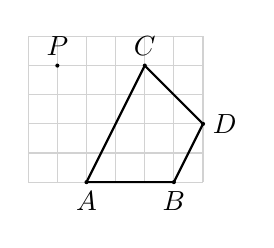
\begin{tikzpicture}[scale=.37]\draw[step=1,gray!35] (0,0) grid (6,5);\coordinate(A)at(2,0);\coordinate(B)at(5,0);\coordinate(C)at(4,4);\coordinate(D)at(6,2);\coordinate(P)at(1,4);\draw[thick](A)--(B)--(D)--(C)--cycle;\foreach \q/\lab/\pos in {A/A/below,B/B/below,C/C/above,D/D/right,P/P/above}{\fill(\q)circle(2pt)node[\pos]{$\lab$};}\end{tikzpicture}
\BookFigure{figures/p037_s08-02.tex}
\end{BookAnswer}

\Needspace{8\baselineskip}

\pdfbookmark[2]{原书第38页}{orig-38}

\subsection*{原书第38页}

% p038_s01
\BookQuestion{二、1}
两个完全相同的三角形一定能拼成（\hspace{1.8em}）。\par
\noindent A. 梯形\par
\noindent B. 平行四边形\par
\noindent C. 长方形\par
\noindent D. 正方形\par
\begin{BookAnswer}
选B。把两个完全相同的三角形的一组对应边重合，其中一个转半周，可以拼成两组对边分别平行的四边形。因此一定能拼成平行四边形；长方形、正方形需要额外角度条件。
\end{BookAnswer}

% p038_s02
\BookQuestion{二、2}
广场花坛的形状是平行四边形，相邻两条边长分别是7米和6米，这个花坛的周长是多少米？（\hspace{1.8em}）\par
\noindent A. 13米\par
\noindent B. 14米\par
\noindent C. 12米\par
\noindent D. 26米\par
\begin{BookAnswer}
选D。平行四边形的两组对边分别相等，周长\((7+6)\times2=26\)米，选D。
\end{BookAnswer}

% p038_s03
\BookQuestion{二、3}
一个等腰直角三角形，其中一个底角是（\hspace{1.8em}）。\par
\noindent A. \(90^\circ\)\par
\noindent B. \(180^\circ\)\par
\noindent C. \(45^\circ\)\par
\noindent D. \(60^\circ\)\par
\begin{BookAnswer}
选C。等腰直角三角形的两个锐角相等，共\(180^\circ-90^\circ=90^\circ\)，每个\(90^\circ\div2=45^\circ\)。
\end{BookAnswer}

% p038_s04
\BookQuestion{二、4}
校门口的电动伸缩门，能自由拉伸开合，它是利用了平行四边形（\hspace{1.8em}）的特性设计的。\par
\noindent A. 稳定性\par
\noindent B. 易变形\par
\noindent C. 对称性\par
\noindent D. 牢固性\par
\BookFigure{figures/p038_s04-01.tex}
\begin{BookAnswer}
选B。平行四边形四条边长度不变时，角度仍可以变化，所以容易变形，适合伸缩门自由拉伸。
\end{BookAnswer}

% p038_s05
\BookQuestion{二、5}
下面各组数据，不能组成三角形的是（\hspace{1.8em}）。\par
\noindent A. 6厘米、6厘米、6厘米\par
\noindent B. 3分米、3分米、6分米\par
\noindent C. 9米、7米、8米\par
\noindent D. 12厘米、6厘米、10厘米\par
\begin{BookAnswer}
选B。三角形任意两边之和必须大于第三边。B中\(3+3=6\)，只能排成一条直线；其余各组的两短边之和都大于最长边。
\end{BookAnswer}

% p038_s06
\BookQuestion{二、6}
裁剪窗花时，把一张平行四边形红纸任意分成两个梯形，这两个梯形的（\hspace{1.8em}）一定相等。\par
\noindent A. 面积\par
\noindent B. 周长\par
\noindent C. 高\par
\noindent D. 上底与下底的和\par
\begin{BookAnswer}
选C。两个梯形的两条底分别落在原平行四边形的同一组平行边上。高是从一条底到另一条底的垂直线段，表示这两条平行线之间的距离；所以两个梯形的高相等。分割线、斜腰或看起来较短的边，都不能直接当作高。面积、周长、两底之和则不一定相等。
\end{BookAnswer}

% p038_s07
\BookQuestion{二、7}
一个三角形中，最小的角是\(46^\circ\)，这个三角形是（\hspace{1.8em}）。\par
\noindent A. 锐角三角形\par
\noindent B. 直角三角形\par
\noindent C. 钝角三角形\par
\noindent D. 无法确定\par
\begin{BookAnswer}
选A。最小角为\(46^\circ\)，其余两个角都不小于\(46^\circ\)。最大角至多\(180^\circ-46^\circ-46^\circ=88^\circ\)，三个角都小于\(90^\circ\)，一定是锐角三角形。
\end{BookAnswer}

% p038_s08
\BookQuestion{三、1}
判断：长方形是特殊的平行四边形，正方形是特殊的长方形。（\hspace{1.8em}）\par
\begin{BookAnswer}
判\(\checkmark\)。长方形的两组对边分别平行，属于平行四边形；正方形四个角都为直角，属于长方形。
\end{BookAnswer}

% p038_s09
\BookQuestion{三、2}
判断：梯形的高一定比它的腰短。（\hspace{1.8em}）\par
\begin{BookAnswer}
判\(\times\)。直角梯形中，与底边垂直的那条腰就等于高，是反例。因此不能说高“一定比腰短”。
\end{BookAnswer}

% p038_s10
\BookQuestion{三、3}
判断：从平行四边形的一个顶点可以向对边作一条高，所以平行四边形有4条高。（\hspace{1.8em}）\par
\begin{BookAnswer}
判\(\times\)。平行四边形的边上有无数个点，都可向对边作垂线段，因此高有无数条，不能只数从顶点画出的几条。对应同一条底，所有高的长度相等；“长度相等”不表示“只有一条”。
\end{BookAnswer}

% p038_s11
\BookQuestion{三、4}
判断：两个完全一样的梯形可以拼成一个平行四边形。（\hspace{1.8em}）\par
\begin{BookAnswer}
判\(\checkmark\)。将两个完全相同的梯形反向拼接，使对应的一条腰重合，可拼成平行四边形，所得两组对边分别平行。
\end{BookAnswer}

% p038_s12
\BookQuestion{三、5}
判断：剪下三角形的一个\(45^\circ\)角，剩下图形的内角和是\(135^\circ\)。（\hspace{1.8em}）\par
\begin{BookAnswer}
判\(\times\)。不能把\(180^\circ\)直接减去剪下的\(45^\circ\)。沿一条线截去一个顶角，剩余部分可能成为四边形，其内角和为\(360^\circ\)；若剪线经过另一个顶点，剩余仍可能是三角形，内角和仍为\(180^\circ\)。
\end{BookAnswer}

% p038_s13
\BookQuestion{三、6}
判断：三角形越大，内角和就越大。（\hspace{1.8em}）\par
\begin{BookAnswer}
判\(\times\)。所有三角形的内角和都是\(180^\circ\)。图形放大或缩小，角度不变。
\end{BookAnswer}

% p038_s14
\BookQuestion{三、7}
判断：有一组对边平行的图形一定是梯形。（\hspace{1.8em}）\par
\begin{BookAnswer}
判\(\times\)。平行四边形也有一组对边平行，不能因此叫梯形。梯形必须是“只有一组对边平行”的四边形。
\end{BookAnswer}

\Needspace{8\baselineskip}

\pdfbookmark[2]{原书第39页}{orig-39}

\subsection*{原书第39页}

% p039_s01
\BookQuestion{四、1（1）}
按要求，画一画。（每两个格点之间的距离为1厘米）（1）以图中线段为三角形的底边，画一个等腰三角形，并画出底边上的高。\par
\BookFigure{figures/p039_s01-01.tex}
\begin{BookAnswer}
先数格找到给定底边的中点；沿经过中点、与底边垂直的方向取顶点，连接顶点与底边两端，得到等腰三角形。用三角尺检验：一条直角边贴底边，另一条直角边经过顶点；画出顶点到垂足的线段，标直角和“高”。原图示例的高经过底边中点，两腰相等。顶点取在底边任一侧，只要满足上述条件，都可以。
\BookFigure{figures/p039_s01-02.tex}
\end{BookAnswer}

% p039_s02
\BookQuestion{四、1（2）}
按要求，画一画。（每两个格点之间的距离为1厘米）（2）画一个梯形，并把梯形分成一个平行四边形和一个三角形。\par
\BookFigure{figures/p039_s02-01.tex}
\begin{BookAnswer}
先画只有一组对边平行的梯形。从一条上底的端点，画一条与不相邻的腰平行的线段，交下底于一点，就能分出一个平行四边形和一个三角形。也可从另一上底端点作对应分割，得到另一种画法。
\BookFigure{figures/p039_s02-02.tex}
\end{BookAnswer}

% p039_s03
\BookQuestion{四、2（1）}
画一画，写一写。（1）利用直尺和圆规，画出以线段\(a\)为底边，线段\(b\)和线段\(c\)为边的三角形。（保留作图痕迹）\par
\BookFigure{figures/p039_s03-01.tex}
\begin{BookAnswer}
先作线段\(AB=a\)。圆规开口取\(b\)，针尖固定在\(A\)画弧；再把开口调为\(c\)，针尖固定在\(B\)，在底边同一侧画弧，两弧交于\(C\)。连接\(AC,BC\)。因为圆规分别保持\(b,c\)的长度，所以\(AC=b,BC=c\)，三条边符合要求。要保留交点附近的弧线，每次画弧时圆规开口不能松动。交点取在底边另一侧也可，得到的两个三角形互为轴对称。
\BookFigure{figures/p039_s03-02.tex}
\end{BookAnswer}

% p039_s04
\BookQuestion{四、2（2）}
（2）根据你画的三角形，请提出一个值得思考的数学问题。（不用解答）\par
\begin{BookAnswer}
问题示例：这个三角形按角分类，属于什么三角形？也可以问：以最长边为底，这条底边上的高在三角形内部还是外部？题目说“不用解答”，提出与所画图形有关的合理问题即可。
\end{BookAnswer}

% p039_s05
\BookQuestion{五、1}
我国古代很早就用方正图形做器物，讲究几何之美。手工课上，李明用一根铁丝先围成了边长9厘米的正方形，如果要用这块铁丝围成一个等边三角形，它的边长是多少厘米？（7分）\par
\begin{BookAnswer}
铁丝总长度不变，先按正方形每边9厘米乘4条边列式，再按等边三角形的3条边平均分。计算时先除以3，再乘4，更便于口算。\[\begin{aligned}&9\times4\div3\\={}&9\div3\times4\\={}&3\times4\\={}&12\text{(厘米)}\end{aligned}\]答：等边三角形的边长是12厘米。\par 另一数量理解：每条原边平均分成3小份，共12小份，每条新边取4小份，直接得到\(9\div3\times4\)。它与上面的简算式一致，不重复列第二遍脱式。
\end{BookAnswer}

\Needspace{8\baselineskip}

\pdfbookmark[2]{原书第40页}{orig-40}

\subsection*{原书第40页}

% p040_s01
\BookQuestion{五、2}
在下面的三角形中，已知\(\angle1=75^\circ\)，\allowbreak{}\(\angle2=60^\circ\)，你能求出\(\angle3\)和\(\angle4\)的度数吗？想一想：\(\angle4\)、\(\angle1\)、\(\angle2\)有什么关系？（7分）\par
\BookFigure{figures/p040_s01-01.tex}
\begin{BookAnswer}
方法一：先用三角形内角和求\(\angle3\)，再用平角求\(\angle4\)。\[\begin{aligned}\angle3&=180^\circ-75^\circ-60^\circ\\&=105^\circ-60^\circ\\&=45^\circ,\\\angle4&=180^\circ-45^\circ\\&=135^\circ.\end{aligned}\]\par 方法二：比较三角形的内角和与底边上的平角，去掉共同的\(\angle3\)，便知\(\angle4\)等于另外两个内角的和。\[\begin{aligned}\angle4&=75^\circ+60^\circ\\&=135^\circ,\\\angle3&=180^\circ-135^\circ\\&=45^\circ.\end{aligned}\]\par 答：\(\angle3=45^\circ,\angle4=135^\circ\)，关系为\(\angle4=\angle1+\angle2\)。这里从已学的内角和、平角推得关系，不要求背诵新的定理名称。
\end{BookAnswer}

% p040_s02
\BookQuestion{五、3}
一根长11厘米的细铁丝，先把它分成三段，再首尾相接围成一个三角形，应该怎样分？小优在2厘米处剪了一刀，再在哪个刻度剪一刀就能围成一个三角形？请你先在图中标出剪的位置，再把想法写出来。（边长为整厘米数）（8分）\par
\BookFigure{figures/p040_s02-01.tex}
\begin{BookAnswer}
方法一：先确定两条余边，再还原剪切位置。第一刀已剪下2厘米，余下两条边的总长是：\[\begin{aligned}&11-2\\={}&9\text{(厘米)}\end{aligned}\]另外两边为整厘米数，和为9、差小于2，只能是4厘米和5厘米。第二刀的位置有两种：\[\begin{aligned}&2+4\\={}&6\text{(厘米)}\end{aligned}\]\[\begin{aligned}&2+5\\={}&7\text{(厘米)}\end{aligned}\]答：可以在6厘米处或7厘米处剪。两种剪法的三边都是2、4、5厘米，满足\(2+4>5\)。\par 方法二：逐一检查整厘米剪切位置。第二刀须落在余下的9厘米部分，可试3至10厘米处。\[\begin{array}{c|c|c}\text{剪切位置}&\text{三边长}&\text{能否围成}\\\hline3&2,1,8&\times\\4&2,2,7&\times\\5&2,3,6&\times\\6&2,4,5&\checkmark\\7&2,5,4&\checkmark\\8&2,6,3&\times\\9&2,7,2&\times\\10&2,8,1&\times\end{array}\]只需检查两条较短边之和是否大于最长边。答：仍为6厘米处或7厘米处；图中两处短线表示备选位置，实际只再剪一处。
\par\smallskip\Needspace{4\baselineskip}\begingroup\small\setlength{\tabcolsep}{3pt}
\noindent\begin{tabularx}{\linewidth}{|*{3}{>{\centering\arraybackslash}X|}}\hline
第二刀刻度（厘米） & 三边长（厘米） & 能否围成\\\hline
\textcolor{answerred}{3} & \textcolor{answerred}{2、1、8} & \textcolor{answerred}{不能}\\\hline
\textcolor{answerred}{4} & \textcolor{answerred}{2、2、7} & \textcolor{answerred}{不能}\\\hline
\textcolor{answerred}{5} & \textcolor{answerred}{2、3、6} & \textcolor{answerred}{不能}\\\hline
\textcolor{answerred}{6} & \textcolor{answerred}{2、4、5} & \textcolor{answerred}{能}\\\hline
\textcolor{answerred}{7} & \textcolor{answerred}{2、5、4} & \textcolor{answerred}{能}\\\hline
\textcolor{answerred}{8} & \textcolor{answerred}{2、6、3} & \textcolor{answerred}{不能}\\\hline
\textcolor{answerred}{9} & \textcolor{answerred}{2、7、2} & \textcolor{answerred}{不能}\\\hline
\textcolor{answerred}{10} & \textcolor{answerred}{2、8、1} & \textcolor{answerred}{不能}\\\hline
\end{tabularx}\par
\endgroup\smallskip
\BookFigure{figures/p040_s02-02.tex}
\end{BookAnswer}

% p040_s03
\BookQuestion{六、思考题}
科技小组制作AI扫地机器人防撞外壳，取用一块直角梯形塑料板，沿一条线段切割，分成一个平行四边形和一个直角三角形。已知梯形下底比上底长3厘米，梯形两条腰长度之和为10厘米。若给分出的直角三角形围一圈防撞条，你能算出这个直角三角形的周长吗？（4分）\par
\BookFigure{figures/p040_s03-01.tex}
\begin{BookAnswer}
右侧切出的直角三角形，一条直角边长等于梯形两底之差3厘米。另外两条边分别与梯形的两腰等长（利用平行四边形对边相等），其和为10厘米。\[\begin{aligned}&10+3\\&=13\text{(厘米)}\end{aligned}\]\par 答：防撞条一圈的长度，即直角三角形的周长，是13厘米。\par 也可从周长转移来理解：原来梯形两腰的总长10厘米都保留到三角形中，再增加两底之差3厘米。
\end{BookAnswer}

\chapter{期中综合}

\Needspace{12\baselineskip}

\section{期中综合素养评价（一）}

\Needspace{8\baselineskip}

\pdfbookmark[2]{原书第41页}{orig-41}

\subsection*{原书第41页}

% p041_s01
\BookQuestion{一、1}
要使\(9\times(\square\div4)=72\)，方框里应该填（\hspace{1.8em}）。\par
\begin{BookAnswer}
填\(32\)。先反向求括号里的商：\(72\div9=8\)；再求被除数：\(8\times4=32\)。检验\(9\times(32\div4)=72\)。
\end{BookAnswer}

% p041_s02
\BookQuestion{一、2}
同一平面内，两条直线的位置关系有（\hspace{1.8em}）和（\hspace{1.8em}）。当两条直线相交成直角时，这两条直线互相（\hspace{1.8em}）。\par
\begin{BookAnswer}
依次填“互相平行、相交、垂直”。同一平面内，两条不同直线要么相交，要么平行；相交成直角时，叫互相垂直。
\end{BookAnswer}

% p041_s03
\BookQuestion{一、3（1）}
根据运算律或性质填空：（1）\(357+168+43+32=(357+\underline{\qquad})+(168+\underline{\qquad})\)。\par
\begin{BookAnswer}
依次填\(43,32\)。把\(357\)与\(43\)凑成400，把\(168\)与\(32\)凑成200；调换加数的位置并改变结合顺序，和不变。
\end{BookAnswer}

% p041_s04
\BookQuestion{一、3（2）}
根据运算律或性质填空：（2）\(125\times(80+8)=125\times\underline{\qquad}+125\times\underline{\qquad}\)。\par
\begin{BookAnswer}
依次填\(80,8\)。乘法分配律是\(a\times(b+c)=a\times b+a\times c\)，所以\(125\times(80+8)=125\times80+125\times8\)。
\end{BookAnswer}

% p041_s05
\BookQuestion{一、3（3）}
根据运算律或性质填空：（3）\(a\times99+a=a\times(\underline{\qquad}+\underline{\qquad})\)。\par
\begin{BookAnswer}
依次填\(99,1\)。单独的\(a\)可写成\(a\times1\)，故\(a\times99+a=a\times(99+1)\)。
\end{BookAnswer}

% p041_s06
\BookQuestion{一、4（1）}
（1）一个平行四边形的两条邻边分别长6厘米和4厘米，它的周长是（\hspace{1.8em}）厘米。\par
\begin{BookAnswer}
填\(20\)。相邻边长6厘米、4厘米，另外两边分别与它们相等，周长\((6+4)\times2=20\)厘米。
\end{BookAnswer}

% p041_s07
\BookQuestion{一、4（2）}
（2）一个等边三角形的周长是27厘米，它的边长是（\hspace{1.8em}）厘米。\par
\begin{BookAnswer}
填\(9\)。等边三角形三边相等，边长\(27\div3=9\)厘米。
\end{BookAnswer}

% p041_s08
\BookQuestion{一、5}
在圆圈里填上“＞”“＜”或“＝”。\(125+25\times4\ \bigcirc\ (125+25)\times4\)；\allowbreak{}\(36\times9+36\times2\ \bigcirc\ 36\times9+2\)；\allowbreak{}\(45\times(12+8)\ \bigcirc\ 45\times12+45\times8\)；\allowbreak{}\(600\div(2\times5)\ \bigcirc\ 600\div2\times5\)。\par
\begin{BookAnswer}
依次填\(<,>,=,<\)。\par \(125+25\times4=225\)，\allowbreak{}\((125+25)\times4=600\)，故\(<\)。\par \(36\times9+36\times2=396\)，\allowbreak{}\(36\times9+2=326\)，故\(>\)。\par 乘法分配律给出\(45\times(12+8)=45\times12+45\times8\)，故\(=\)。\par \(600\div(2\times5)=60\)，\allowbreak{}\(600\div2\times5=1500\)，故\(<\)。
\end{BookAnswer}

% p041_s09
\BookQuestion{一、6}
一个直角三角形中，有一个锐角是\(45^\circ\)，另一个锐角是（\hspace{1.8em}），按边分它是（\hspace{1.8em}）三角形。把这样两个完全一样的三角形拼成一个大三角形，大三角形的内角和是（\hspace{1.8em}）；拼成一个正方形，正方形的内角和是（\hspace{1.8em}）。\par
\begin{BookAnswer}
依次填\(45^\circ\)、等腰、\(180^\circ\)、\(360^\circ\)。另一个锐角\(180^\circ-90^\circ-45^\circ=45^\circ\)。两锐角相等，所以是等腰三角形。拼成的大三角形内角和仍为\(180^\circ\)；正方形有4个直角，内角和\(90^\circ\times4=360^\circ\)。
\end{BookAnswer}

\Needspace{8\baselineskip}

\pdfbookmark[2]{原书第42页}{orig-42}

\subsection*{原书第42页}

% p042_s01
\BookQuestion{一、7}
商店购进6箱火龙果，每箱24千克，如果分装成每袋8千克，一共可以分装（\hspace{1.8em}）袋；把这些火龙果按每袋12元售卖，全部售出一共收入（\hspace{1.8em}）元。\par
\begin{BookAnswer}
依次填\(18,216\)。袋数先利用24除以8求每箱袋数，计算更简便；收入按单价乘袋数。\[\begin{aligned}&24\times6\div8\\={}&24\div8\times6\\={}&3\times6\\={}&18\text{(袋)}\\&12\times18\\={}&216\text{(元)}\end{aligned}\]
\end{BookAnswer}

% p042_s02
\BookQuestion{一、8}
右图中，有（\hspace{1.8em}）个三角形，（\hspace{1.8em}）个平行四边形，（\hspace{1.8em}）个梯形。\par
\BookFigure{figures/p042_s02-01.tex}
\begin{BookAnswer}
依次填\(3,3,4\)。三角形有左、中、右3个。平行四边形按两条底边之间的两条同方向斜边配对，共3个。梯形按大小和位置逐一检查，共4个；只数“只有一组对边平行”的图形，不能把平行四边形重复计入。
\end{BookAnswer}

% p042_s03
\BookQuestion{二、1}
与\(720\div(8\times9)\)结果相等的算式是（\hspace{1.8em}）。\par
\noindent A. \(720\div8\times9\)\par
\noindent B. \(720\div8\div9\)\par
\noindent C. \(720\times8\div9\)\par
\noindent D. \(720\div9\times8\)\par
\begin{BookAnswer}
选B。除以两个数的积，等于依次除以这两个数：\(720\div(8\times9)=720\div8\div9\)。
\end{BookAnswer}

% p042_s04
\BookQuestion{二、2}
\(25\times(a+4)\)与\(25\times a+25\)的结果相差（\hspace{1.8em}）。\par
\noindent A. \(24a\)\par
\noindent B. \(a\)\par
\noindent C. 4\par
\noindent D. 75\par
\begin{BookAnswer}
选D。\(25\times(a+4)=25\times a+100\)，另一个式子为\(25\times a+25\)，相差\(100-25=75\)。
\end{BookAnswer}

% p042_s05
\BookQuestion{二、3}
在同一平面内，如果直线\(a\)垂直于直线\(b\)，直线\(b\)垂直于直线\(c\)，那么直线\(a\)和\(c\)（\hspace{1.8em}）。\par
\noindent A. 互相平行\par
\noindent B. 互相垂直\par
\noindent C. 相交但不垂直\par
\noindent D. 无法确定\par
\begin{BookAnswer}
选A。同一平面内，垂直于同一条直线的两条不同直线互相平行，所以\(a\parallel c\)。
\end{BookAnswer}

% p042_s06
\BookQuestion{二、4}
下面每组中的三根小棒，能围成三角形的是（\hspace{1.8em}）（单位：厘米）。\par
\noindent A. 4、5、9\par
\noindent B. 3、4、8\par
\noindent C. 5、6、10\par
\noindent D. 2、2、5\par
\begin{BookAnswer}
选C。检验两短边之和：A为\(4+5=9\)，B为\(3+4<8\)，D为\(2+2<5\)，均不成立；C有\(5+6>10\)，能围成三角形。
\end{BookAnswer}

% p042_s07
\BookQuestion{二、5}
一个三角形的最小角是\(50^\circ\)，这个三角形一定是（\hspace{1.8em}）。\par
\noindent A. 锐角三角形\par
\noindent B. 直角三角形\par
\noindent C. 钝角三角形\par
\noindent D. 无法判断\par
\begin{BookAnswer}
选A。最小角50度，其余角都至少50度，最大角至多\(180^\circ-50^\circ-50^\circ=80^\circ\)，所以一定是锐角三角形。
\end{BookAnswer}

% p042_s08
\BookQuestion{三、1}
直接写得数。\(25\times3\times4=\)，\allowbreak{}\(125\times8=\)，\allowbreak{}\(23\times10=\)，\allowbreak{}\(200-100\div10=\)；\allowbreak{}\(360\div60=\)，\allowbreak{}\(11\times20=\)，\allowbreak{}\((12+8)\times5=\)，\allowbreak{}\(80\div(8\times2)=\)。\par
\begin{BookAnswer}
按题面顺序，得\(300,1000,230,190;6,220,100,5\)。\par \(25\times3\times4=(25\times4)\times3=300\)；\allowbreak{}\(125\times8=1000\)；\allowbreak{}\(23\times10=230\)；\allowbreak{}\(200-100\div10=200-10=190\)。\par \(360\div60=6\)；\allowbreak{}\(11\times20=220\)；\allowbreak{}\((12+8)\times5=20\times5=100\)；\allowbreak{}\(80\div(8\times2)=80\div16=5\)。
\end{BookAnswer}

% p042_s09
\BookQuestion{三、2（1）}
计算下面各题，能简算的要简算。\(640\div[16\times(19-14)]\)。\par
\begin{BookAnswer}
先求最内层的差，再把16与5相乘凑成整十除数80，直接相除。\[\begin{aligned}&640\div[16\times(19-14)]\\={}&640\div[16\times5]\\={}&640\div80\\={}&8\end{aligned}\]
\end{BookAnswer}

% p042_s10
\BookQuestion{三、2（2）}
计算下面各题，能简算的要简算。\(25\times32\times25\)。\par
\begin{BookAnswer}
把32拆成\(4\times8\)，运用乘法结合律，分别凑成整百数。\[\begin{aligned}&25\times32\times25\\&=(25\times4)\times(8\times25)\\&=100\times200\\&=20000.\end{aligned}\]
\end{BookAnswer}

% p042_s11
\BookQuestion{三、2（3）}
计算下面各题，能简算的要简算。\(99\times47+47\)。\par
\begin{BookAnswer}
把最后一个47看作\(1\times47\)，运用乘法分配律，把99个47和1个47合成100个47。\[\begin{aligned}&99\times47+47\\={}&(99+1)\times47\\={}&100\times47\\={}&4700\end{aligned}\]另一写法“先按100个47算，减去1个47后再加回”反映同一凑整结构，不另算一种解法。
\end{BookAnswer}

% p042_s12
\BookQuestion{三、2（4）}
计算下面各题，能简算的要简算。\(35\times98\)。\par
\begin{BookAnswer}
用乘法分配律，把98看作\(100-2\)。\[\begin{aligned}&35\times98\\={}&35\times(100-2)\\={}&35\times100-35\times2\\={}&3500-70\\={}&3430\end{aligned}\]
\end{BookAnswer}

\Needspace{8\baselineskip}

\pdfbookmark[2]{原书第43页}{orig-43}

\subsection*{原书第43页}

% p043_s01
\BookQuestion{四、1}
过直线外的点\(A\)，画已知直线的垂线和平行线。（4分）\par
\BookFigure{figures/p043_s01-01.tex}
\begin{BookAnswer}
先画垂线：把三角尺一条直角边靠在已知直线上，沿直线平移三角尺，使另一条直角边经过\(A\)，再沿这条边画线，垂足处标直角。再借助直尺推移三角尺，过\(A\)画已知直线的平行线。两条红线都要经过\(A\)；平行线与原直线不相交，垂线与原直线交成直角。
\BookFigure{figures/p043_s01-02.tex}
\end{BookAnswer}

% p043_s02
\BookQuestion{四、2}
在下面的方格纸上（每个小方格边长1厘米），画一个底边为5厘米、高为3厘米的平行四边形，并画出它的一条高。（4分）\par
\BookFigure{figures/p043_s02-01.tex}
\begin{BookAnswer}
先在同一格线上取长5格的底边；再在与它相距3格、互相平行的另一格线上取长5格的对边，将对应端点连起来。检查两组对边分别平行，才是平行四边形。用三角尺从上边一点向底边作垂线段，标直角与“高3厘米”。这里3格按垂直方向数，不是沿斜边数。同一底上的高都长3厘米，上边可换一个点另作一条高。
\BookFigure{figures/p043_s02-02.tex}
\end{BookAnswer}

% p043_s03
\BookQuestion{五、1}
工程队修一条公路，原计划每天修120米，8天修完。实际提前2天完成，实际平均每天修多少米？（5分）\par
\begin{BookAnswer}
方法一：路长不变；列式后先算120除以6，凑成整十数20。\par \[\begin{aligned}&120\times8\div(8-2)\\={}&120\times8\div6\\={}&120\div6\times8\\={}&20\times8\\={}&160\text{(米)}\end{aligned}\]答：实际平均每天修160米。\par 方法二：把原来2天的任务平均增加到实际6天，增加部分也先算120除以6。\par \[\begin{aligned}&120+120\times2\div(8-2)\\={}&120+120\times2\div6\\={}&120+120\div6\times2\\={}&120+20\times2\\={}&120+40\\={}&160\text{(米)}\end{aligned}\]答：实际平均每天修160米。
\end{BookAnswer}

% p043_s04
\BookQuestion{五、2}
一个等腰三角形的两条边长分别是6厘米和8厘米。这个等腰三角形的周长可能是多少厘米？（5分）\par
\begin{BookAnswer}
“两条边长6厘米、8厘米”没有指定哪条是底，必须分两种情况。\par 情况一：6厘米为腰，8厘米为底。\[\begin{aligned}&6\times2+8\\&=12+8\\&=20\text{(厘米)}\end{aligned}\]\par 情况二：8厘米为腰，6厘米为底。\[\begin{aligned}&8\times2+6\\&=16+6\\&=22\text{(厘米)}\end{aligned}\]\par 两种都能成三角形，因为\(6+6>8\)、\(8+8>6\)。答：周长可能是20厘米或22厘米。这是两种可能情况，不能只写其中一种。
\end{BookAnswer}

\Needspace{8\baselineskip}

\pdfbookmark[2]{原书第44页}{orig-44}

\subsection*{原书第44页}

% p044_s01
\BookQuestion{五、3}
一根铁丝可以围成一个边长9厘米的正方形，如果改围成一个等边三角形，那么这个等边三角形的边长是多少厘米？（5分）\par
\begin{BookAnswer}
铁丝总长度不变，先按正方形每边9厘米乘4条边列式，再按等边三角形的3条边平均分。计算时先除以3，再乘4，更便于口算。\[\begin{aligned}&9\times4\div3\\={}&9\div3\times4\\={}&3\times4\\={}&12\text{(厘米)}\end{aligned}\]答：等边三角形的边长是12厘米。\par 另一数量理解：每条原边平均分成3小份，共12小份，每条新边取4小份，直接得到\(9\div3\times4\)。它与上面的简算式一致，不重复列第二遍脱式。
\end{BookAnswer}

% p044_s02
\BookQuestion{五、4（1）}
超市举行“酸奶促销活动”：每瓶酸奶6元，买5瓶送1瓶。李阿姨需要买24瓶酸奶送给敬老院。（1）李阿姨实际需要付多少瓶的钱？（5分）\par
\begin{BookAnswer}
“买5送1”表示每组得到6瓶，只付5瓶的钱。\par 方法一：直接求付费瓶数。\[\begin{aligned}&5\times[24\div(5+1)]\\&=5\times[24\div6]\\&=5\times4\\&=20\text{(瓶)}\end{aligned}\]\par 方法二：先求赠送瓶数，再从总瓶数中扣去。\[\begin{aligned}&24-24\div6\\&=24-4\\&=20\text{(瓶)}\end{aligned}\]\par 答：实际要付20瓶的钱。
\end{BookAnswer}

% p044_s03
\BookQuestion{五、4（2）}
超市举行“酸奶促销活动”：每瓶酸奶6元，买5瓶送1瓶。李阿姨需要买24瓶酸奶送给敬老院。（2）她一共要付多少元？（5分）\par
\begin{BookAnswer}
方法一：每瓶价格乘付费瓶数。\[\begin{aligned}&6\times20\\={}&120\text{(元)}\end{aligned}\]答：一共要付120元。\par 方法二：从24瓶全价扣去赠品价格，反用乘法分配律先算付费瓶数。\[\begin{aligned}&6\times24-6\times(24\div6)\\={}&6\times24-6\times4\\={}&6\times(24-4)\\={}&6\times20\\={}&120\text{(元)}\end{aligned}\]答：一共要付120元。
\end{BookAnswer}

% p044_s04
\BookQuestion{五、5}
实验小学开展“废纸回收，保护环境”活动。四年级回收废纸275千克，五年级回收的废纸比四年级的2倍少50千克。每回收25千克废纸可以挽救1棵大树。两个年级一共可以挽救多少棵大树？（6分）\par
\begin{BookAnswer}
方法一：先求五年级质量，按总回收量列式，再把275与500分别除以25。\par \[\begin{aligned}&[275+(275\times2-50)]\div25\\={}&[275+(550-50)]\div25\\={}&[275+500]\div25\\={}&275\div25+500\div25\\={}&11+20\\={}&31\text{(棵)}\end{aligned}\]答：两个年级一共可以挽救31棵大树。\par 方法二：先按四年级的3份算，再扣去少回收50千克对应的棵数。\par \[\begin{aligned}&275\div25\times3-50\div25\\={}&11\times3-2\\={}&33-2\\={}&31\text{(棵)}\end{aligned}\]答：两个年级一共可以挽救31棵大树。\par 方法三：两个年级分别换算棵数，再相加。\par \[\begin{aligned}&275\div25+(275\times2-50)\div25\\={}&11+(550-50)\div25\\={}&11+500\div25\\={}&11+20\\={}&31\text{(棵)}\end{aligned}\]答：两个年级一共可以挽救31棵大树。
\end{BookAnswer}

\Needspace{12\baselineskip}

\section{期中综合素养评价（二）}

\Needspace{8\baselineskip}

\pdfbookmark[2]{原书第45页}{orig-45}

\subsection*{原书第45页}

% p045_s01
\BookQuestion{一、1}
给算式\(200+370-295\div5\)添上括号，使它的运算顺序变成先算减法，再算加法，最后算除法：（\hspace{1.8em}）。\par
\begin{BookAnswer}
填\([200+(370-295)]\div5\)。题目要求先算减法，把\(370-295\)括起；再与200相加，把这个和整体放进中括号；最后除以5。
\end{BookAnswer}

% p045_s02
\BookQuestion{一、2}
装修公司要给一个面积为96平方米的会议厅铺防滑地砖，每平方米的地砖和施工费用合计48元，完成这个会议厅的地砖铺设总共需要花费（\hspace{1.8em}）元。\par
\begin{BookAnswer}
填\(4608\)。每平方米48元，96平方米的费用为\(48\times96=48\times(100-4)=4800-192=4608\)元。乘法顺序按“每平方米费用×平方米数”。
\end{BookAnswer}

% p045_s03
\BookQuestion{一、3}
钟面上（\hspace{1.8em}）时整和（\hspace{1.8em}）时整，时针和分针互相垂直。\par
\begin{BookAnswer}
依次填\(3,9\)。整时的分针指向12。时针指向3或9时，与12相差3个大格，即\(30^\circ\times3=90^\circ\)，所以互相垂直。
\end{BookAnswer}

% p045_s04
\BookQuestion{一、4}
小新用加法运算律写了一个等式：\(\square2+4\square=\square8+5\square\)。如果这两个加数的和是100，那么这两个加数分别是（\hspace{1.8em}）和（\hspace{1.8em}）。\par
\begin{BookAnswer}
两个加数为\(52,48\)，四个方框依次填\(5,8,4,2\)。算式应用加法交换律，故\(\square2\)与\(5\square\)相同、\(4\square\)与\(\square8\)相同，先得到52和48。检验\(52+48=100\)。
\end{BookAnswer}

% p045_s05
\BookQuestion{一、5（1）}
根据运算律填一填。（1）\(175+264+225+136=(\square\bigcirc\square)\bigcirc(\square\bigcirc\square)\)。\par
\begin{BookAnswer}
一种填写为\((175+225)+(264+136)\)。把175和225凑成400，把264和136也凑成400，应用加法交换律和结合律，总和为800。两组的前后互换也正确。
\end{BookAnswer}

% p045_s06
\BookQuestion{一、5（2）}
根据运算律填一填。（2）\(\square\times99+\square\times\square=a\times(\square\bigcirc1)\)。\par
\begin{BookAnswer}
依次填\(a,a,1,99,+\)。式子为\(a\times99+a\times1=a\times(99+1)\)，这是乘法分配律的逆用。
\end{BookAnswer}

% p045_s07
\BookQuestion{一、6}
印刷厂工人每小时能印刷300份报纸，每天工作8小时，一周（5个工作日）能印刷（\hspace{1.8em}）份报纸。\par
\begin{BookAnswer}
填\(12000\)。每小时300份，按“每份数\(\times\)份数”列式，用乘法结合律先求总工作时间：\[\begin{aligned}&300\times8\times5\\={}&300\times(8\times5)\\={}&300\times40\\={}&12000\text{(份)}\end{aligned}\]一周只算5个工作日。
\end{BookAnswer}

% p045_s08
\BookQuestion{一、7}
在圆圈里填上“＞”“＜”或“＝”。\(38\times(5+6)\ \bigcirc\ 38\times5+6\)，\allowbreak{}\(420\div21\ \bigcirc\ 420\div7\div3\)；\allowbreak{}\(78\times199\ \bigcirc\ 78\times200-1\)，\allowbreak{}\(74\times10\times2\ \bigcirc\ 74\times12\)；\allowbreak{}\(65\times24\ \bigcirc\ 65\times4\times20\)，\allowbreak{}\(107\times5\ \bigcirc\ 105\times7\)。\par
\begin{BookAnswer}
依次填\(>,=,<,>,<,<\)。\par \(38\times(5+6)=418>196=38\times5+6\)。\par \(420\div21=420\div7\div3=20\)。\par \(78\times199=15522<15599=78\times200-1\)，少的是78而不是1。\par \(74\times10\times2=1480>888=74\times12\)。\par \(65\times24=1560<65\times4\times20=5200\)。\par \(107\times5=535<735=105\times7\)。
\end{BookAnswer}

% p045_s09
\BookQuestion{一、8}
斑马线中的每一组白线可以看作互相（\hspace{1.8em}）的线段。\par
\begin{BookAnswer}
填“平行”。一组斑马线中的白线沿同一方向、不会相交，可看作互相平行的线段。
\end{BookAnswer}

% p045_s10
\BookQuestion{一、9}
一个等腰三角形的木板，顶角是底角的4倍，底角是（\hspace{1.8em}）°。\par
\begin{BookAnswer}
填\(30^\circ\)。把一个底角看成1份，另一个底角也是1份，顶角为4份，共6份。每份\(180^\circ\div(1+1+4)=30^\circ\)。
\end{BookAnswer}

\Needspace{8\baselineskip}

\pdfbookmark[2]{原书第46页}{orig-46}

\subsection*{原书第46页}

% p046_s01
\BookQuestion{一、10}
在直角三角形\(ABC\)中（单位：厘米），\allowbreak{}\(AC\)边上的高是（\hspace{1.8em}）厘米，\allowbreak{}\(AB\)边上的高是（\hspace{1.8em}）厘米。三角形（\hspace{1.8em}）中（\hspace{1.8em}）边上的高是1.9厘米。\par
\BookFigure{figures/p046_s01-01.tex}
\begin{BookAnswer}
依次填\(1.8,4,BCD,BC\)。先找底，再找“从对面顶点到这条底所在直线”的垂线段，不能看哪一条边画得较斜或较短。\par 以\(AC\)为底，高是\(BD\)，按标注为1.8厘米；以\(AB\)为底，高是与它垂直的\(BC\)，长4厘米。直角三角形的两条直角边可以互为底和高。\(D\)到\(BC\)的垂线段标为1.9厘米，因此在三角形\(BCD\)中，以\(BC\)为底，对应高按图为1.9厘米。\par 原图的尺寸不能同时成立：\(D\)到\(BC\)的垂直线段长1.9厘米，却比从\(D\)到直线上一点\(B\)的线段\(DB=1.8\)厘米还长，违反“垂线段最短”。以上只按题图标示识别底高关系，不能据这些冲突尺寸另作精确图。
\end{BookAnswer}

% p046_s02
\BookQuestion{二、1}
下列算式中正确的是（\hspace{1.8em}）。\par
\noindent A. \(480\div12\times4=480\div(12\times4)\)\par
\noindent B. \(630\div(7\times9)=630\div7\times9\)\par
\noindent C. \(25\times(40+8)=25\times40+8\)\par
\noindent D. \(900\div25\div4=900\div(25\times4)\)\par
\begin{BookAnswer}
选D。\(900\div25\div4=900\div(25\times4)=9\)，符合连续除法的性质。A把“除后乘4”改成“再除4”；B同样把除以9改成乘9；C漏乘了括号里的8。
\end{BookAnswer}

% p046_s03
\BookQuestion{二、2}
一幢大楼有25层，每层有18扇窗户，每扇窗户有4块玻璃，这幢大楼一共有多少块玻璃？下面列式正确的是（\hspace{1.8em}）。\par
\noindent A. \(25\times(18+4)\)\par
\noindent B. \(25\times18\times4\)\par
\noindent C. \(25\times18-4\)\par
\noindent D. \(25\times18\div4\)\par
\begin{BookAnswer}
选B。每扇4块，先求18扇一层的玻璃数，再求25层：\[\begin{aligned}&4\times18\times25\\={}&(4\times25)\times18\\={}&100\times18\\={}&1800\text{(块)}\end{aligned}\]选项\(25\times18\times4\)与此式由乘法交换律相等。
\end{BookAnswer}

% p046_s04
\BookQuestion{二、3}
下列各组小棒中（单位：厘米），能围成三角形的是（\hspace{1.8em}）。\par
\noindent A. 3、4、7\par
\noindent B. 2、3、6\par
\noindent C. 6、6、10\par
\noindent D. 5、2、2\par
\begin{BookAnswer}
选C。C中两短边之和\(6+6=12>10\)，能围成三角形。A为\(3+4=7\)，B为\(2+3<6\)，D为\(2+2<5\)，均不行。
\end{BookAnswer}

% p046_s05
\BookQuestion{二、4}
\(34\times(\triangle+\square)=34\times\triangle+34\times\square\)，这是运用了（\hspace{1.8em}）。\par
\noindent A. 加法交换律\par
\noindent B. 乘法结合律\par
\noindent C. 乘法分配律\par
\noindent D. 乘法交换律\par
\begin{BookAnswer}
选C。\(34\times(\triangle+\square)=34\times\triangle+34\times\square\)，把34分别乘两个加数，应用的是乘法分配律。
\end{BookAnswer}

% p046_s06
\BookQuestion{二、5}
在梯形里画一条线段，把梯形分成两个图形，这两个图形不可能是（\hspace{1.8em}）。\par
\noindent A. 两个梯形\par
\noindent B. 两个三角形\par
\noindent C. 两个平行四边形\par
\noindent D. 一个三角形和一个平行四边形\par
\begin{BookAnswer}
选C。一刀分成两个平行四边形，会使外部图形也具有两组对边分别平行，与原梯形“只有一组对边平行”矛盾。因此不可能分成两个平行四边形；其余三类均能画出实例。
\end{BookAnswer}

% p046_s07
\BookQuestion{三、1}
直接写得数。\(12\times9=\)，\allowbreak{}\(152\times4=\)，\allowbreak{}\(600\div25=\)，\allowbreak{}\((12+8)\times5=\)，\allowbreak{}\(397-23\times6=\)；\allowbreak{}\(125\times8=\)，\allowbreak{}\(24\times5=\)，\allowbreak{}\(480\div80\div6=\)，\allowbreak{}\(49\times31\approx\)，\allowbreak{}\(61\times95\approx\)。\par
\begin{BookAnswer}
第一行依次为\(108,608,24,100,259\)。\par 第二行依次为\(1000,120,1,1500,6000\)。\par \(12\times9=108\)，\allowbreak{}\(152\times4=608\)，\allowbreak{}\(600\div25=600\times4\div100=24\)，\allowbreak{}\((12+8)\times5=100\)。\par \(397-23\times6=397-138=259\)；\allowbreak{}\(125\times8=1000\)，\allowbreak{}\(24\times5=120\)，\allowbreak{}\(480\div80\div6=6\div6=1\)。\par 估算：\(49\times31\approx50\times30=1500\)，\allowbreak{}\(61\times95\approx60\times100=6000\)。估算写约等号，不能把估计值当精确值。
\end{BookAnswer}

% p046_s08
\BookQuestion{三、2（1）}
计算下面各题，能简算的要简算。\(480-12\times(360\div18)\)。\par
\begin{BookAnswer}
先算括号内除法。\[\begin{aligned}&480-12\times(360\div18)\\&=480-12\times20\\&=480-240\\&=240.\end{aligned}\]
\end{BookAnswer}

% p046_s09
\BookQuestion{三、2（2）}
计算下面各题，能简算的要简算。\(45\times[(63+177)\div24]\)。\par
\begin{BookAnswer}
按括号层次计算。\[\begin{aligned}&45\times[(63+177)\div24]\\&=45\times[240\div24]\\&=45\times10\\&=450.\end{aligned}\]
\end{BookAnswer}

% p046_s10
\BookQuestion{三、2（3）}
计算下面各题，能简算的要简算。\(136\times101-136\)。\par
\begin{BookAnswer}
把单独的136看作\(136\times1\)，运用乘法分配律逆用凑出100。\[\begin{aligned}&136\times101-136\\={}&136\times(101-1)\\={}&136\times100\\={}&13600\end{aligned}\]展开成“13600加136再减136”是同一凑整结构的另写法，不另列一种解法。
\end{BookAnswer}

% p046_s11
\BookQuestion{三、2（4）}
计算下面各题，能简算的要简算。\(125\times48\)。\par
\begin{BookAnswer}
方法一：拆48为\(8\times6\)，运用乘法结合律。\[\begin{aligned}&125\times48\\={}&125\times(8\times6)\\={}&(125\times8)\times6\\={}&1000\times6\\={}&6000\end{aligned}\]\par 方法二：把48看作\(50-2\)，用乘法分配律。\[\begin{aligned}&125\times48\\={}&125\times(50-2)\\={}&125\times50-125\times2\\={}&6250-250\\={}&6000\end{aligned}\]
\end{BookAnswer}

\Needspace{8\baselineskip}

\pdfbookmark[2]{原书第47页}{orig-47}

\subsection*{原书第47页}

% p047_s01
\BookQuestion{四、1}
小区要在一条笔直的公路旁建一个快递驿站，驿站的位置在点\(A\)处（如下图）。现在要从驿站修一条最短的小路连接到公路上，方便居民取快递，请你画出这条小路。（4分）\par
\BookFigure{figures/p047_s01-01.tex}
\begin{BookAnswer}
把三角尺一条直角边靠在公路近侧边缘所在直线上，平移到另一条直角边经过\(A\)，从\(A\)沿这条边画到公路边缘，垂足处标直角。点到直线的垂线段最短，所以这是最短小路。小路的终点是公路边缘，不必延伸到公路中心或另一侧。
\BookFigure{figures/p047_s01-02.tex}
\end{BookAnswer}

% p047_s02
\BookQuestion{四、2}
用直尺和圆规画一个以线段\(AB\)为边的等边三角形。（4分）\par
\BookFigure{figures/p047_s02-01.tex}
\begin{BookAnswer}
圆规开口取\(AB\)的长度，针尖先固定在\(A\)画弧，再保持同样开口、固定在\(B\)画弧，两弧交于\(C\)。连接\(AC,BC\)，并保留交点附近的两段弧。因为\(AC\)与\(BC\)都是按同一个长度\(AB\)画出的，所以\(AB=AC=BC\)，得到等边三角形。若两弧暂未相交，应延长弧线，不能任意改变圆规开口。交点取在\(AB\)的另一侧同样成立。
\BookFigure{figures/p047_s02-02.tex}
\end{BookAnswer}

% p047_s03
\BookQuestion{五、1}
求出\(\angle1\)的度数。（5分）\par
\BookFigure{figures/p047_s03-01.tex}
\begin{BookAnswer}
方法一：先用平角求\(\angle2\)，再用三角形内角和求\(\angle1\)。\[\begin{aligned}\angle2&=180^\circ-138^\circ\\&=42^\circ,\\\angle1&=180^\circ-61^\circ-42^\circ\\&=119^\circ-42^\circ\\&=77^\circ.\end{aligned}\]\par 方法二：把三角形的三个内角与底边上的平角比一比，去掉两边共同的\(\angle2\)，可知\(\angle1\)和\(61^\circ\)合起来等于\(138^\circ\)。\[\begin{aligned}\angle1&=138^\circ-61^\circ\\&=77^\circ.\end{aligned}\]\par 答：\(\angle1=77^\circ\)。第二法的依据仍是已学的“内角和180度”与“平角180度”。
\end{BookAnswer}

% p047_s04
\BookQuestion{五、2}
两架客机从同一机场向相反方向起飞，甲机巡航速度为800千米/时，乙机巡航速度为850千米/时。两架飞机同时飞出2小时后，它们之间相距多少千米？（先画图整理条件和问题，再解答）（6分）\par
\begin{BookAnswer}
画图：以机场为共同起点，向相反方向画两段路程；甲段标\(800\times2\)，乙段标\(850\times2\)，两段合起来就是相距的路程。\par 方法一：先求速度和，再乘共同时间。\[\begin{aligned}&(800+850)\times2\\&=1650\times2\\&=3300\text{(千米)}\end{aligned}\]\par 方法二：分别求两架飞机的路程，再相加。\[\begin{aligned}&800\times2+850\times2\\&=1600+1700\\&=3300\text{(千米)}\end{aligned}\]\par 答：2小时后两架飞机之间相距3300千米。
\BookFigure{figures/p047_s04-01.tex}
\end{BookAnswer}

\Needspace{8\baselineskip}

\pdfbookmark[2]{原书第48页}{orig-48}

\subsection*{原书第48页}

% p048_s01
\BookQuestion{五、3}
猕猴桃每100克大约含62毫克维生素C。成年人每日需摄入超过100毫克维生素C。李叔叔今天吃了200克猕猴桃，能满足一天的维生素C摄入量吗？（6分）\par
\begin{BookAnswer}
每100克大约含62毫克，200克里有\(200\div100=2\)份。\[\begin{aligned}&62\times(200\div100)\\={}&62\times2\\={}&124\text{(毫克)}\end{aligned}\]也可以用重复加法表示两份：\(62+62=124\text{(毫克)}\)，这是相同数量关系的两种表达，不另算独立思路。按题目给定的含量估计，约摄入124毫克维生素C，\allowbreak{}\(124>100\)。答：能满足题目所给的一天维生素C摄入量要求。
\end{BookAnswer}

% p048_s02
\BookQuestion{五、4（1）}
学校有三个热门社团，航模社团报名128人，编程社团报名275人，书法社团报名172人。（1）三个社团一共有多少人报名？（4分）\par
\begin{BookAnswer}
把航模、编程、书法三个社团人数相加，用加法交换律和结合律先凑300：\[\begin{aligned}&128+275+172\\={}&(128+172)+275\\={}&300+275\\={}&575\text{(人)}\end{aligned}\]答：三个社团一共有575人报名。
\end{BookAnswer}

% p048_s03
\BookQuestion{五、4（2）}
学校有三个热门社团，航模社团报名128人，编程社团报名275人，书法社团报名172人。（2）编程社团的报名人数，比航模和书法两个社团报名人数的总和少多少人？（4分）\par
\begin{BookAnswer}
方法一：先求航模和书法两社团总人数，再与编程社团比较。\[\begin{aligned}&128+172-275\\&=300-275\\&=25\text{(人)}\end{aligned}\]\par 方法二：先用编程人数减去书法人数，余下部分再与航模人数比较。\[\begin{aligned}&128-(275-172)\\&=128-103\\&=25\text{(人)}\end{aligned}\]\par 答：编程社团比另外两个社团人数的总和少25人。
\end{BookAnswer}

% p048_s04
\BookQuestion{五、5}
国庆节期间，学校组织四年级90名学生和20位老师去公园玩。用3000元购票后还剩多少元？（6分）\par
\par\smallskip\Needspace{4\baselineskip}\begingroup\small\setlength{\tabcolsep}{3pt}
\noindent\textbf{公园门票收费标准}\par\smallskip
\noindent\begin{tabularx}{\linewidth}{|*{3}{>{\centering\arraybackslash}X|}}\hline
季节 & 成人 & 儿童\\\hline
旺季 & 30元 & 20元\\\hline
淡季 & 15元 & 10元\\\hline
\end{tabularx}\par
\noindent 旺季：4月1日～10月31日\par
\noindent 淡季：11月1日～3月31日\par
\endgroup\smallskip
\begin{BookAnswer}
国庆节在10月，按旺季票价：儿童每人20元，成人每人30元。\par 方法一：先求两类票总费用，再从3000元中扣去。\[\begin{aligned}&3000-(20\times90+30\times20)\\={}&3000-(1800+600)\\={}&3000-2400\\={}&600\text{(元)}\end{aligned}\]答：还剩600元。\par 方法二：先买儿童票，再买成人票，依次扣款。\[\begin{aligned}&3000-20\times90-30\times20\\={}&3000-1800-600\\={}&1200-600\\={}&600\text{(元)}\end{aligned}\]答：还剩600元。\par 方法三：先按110人全买儿童票，再补老师的差价。\[\begin{aligned}&3000-20\times(90+20)-(30-20)\times20\\={}&3000-20\times110-10\times20\\={}&3000-2200-200\\={}&800-200\\={}&600\text{(元)}\end{aligned}\]答：还剩600元。
\end{BookAnswer}

\chapter{第六单元}

\Needspace{12\baselineskip}

\section{第六单元素养评价（A）}

\Needspace{8\baselineskip}

\pdfbookmark[2]{原书第49页}{orig-49}

\subsection*{原书第49页}

% p049_s01
\BookQuestion{一、1}
中国国家博物馆遵循“开门办馆”的理念，分期分批对社会公布馆藏藏品目录，第一期共公布藏品约30.64万件。横线上的小数读作（\hspace{1.8em}），这个小数的计数单位是（\hspace{1.8em}），它有（\hspace{1.8em}）个这样的计数单位。\par
\begin{BookAnswer}
依次填“三十点六四、\(0.01\)、\(3064\)”。整数部分30按整数读法读“三十”，小数部分按数位逐个读“六、四”。30.64写到百分位，计数单位是百分之一，即0.01。3个十相当于3000个0.01，6个十分之一相当于60个0.01，再加4个0.01，共\(3000+60+4=3064\)个。
\end{BookAnswer}

% p049_s02
\BookQuestion{一、2}
一个小数由8个0.1和7个0.01组成，这个小数是（\hspace{1.8em}），再加上（\hspace{1.8em}）个\(\frac1{100}\)就是1。\par
\begin{BookAnswer}
依次填\(0.87,13\)。\(8\)个\(0.1\)是\(0.8\)，\allowbreak{}\(7\)个\(0.01\)是\(0.07\)，合为\(0.87\)。把1写成\(1.00\)，还差\(1.00-0.87=0.13\)，即13个\(\frac1{100}\)。
\end{BookAnswer}

% p049_s03
\BookQuestion{一、3}
把168000改写成用“万”作单位的数是（\hspace{1.8em}）万，保留整数约是（\hspace{1.8em}）万；把995000000改写成以“亿”为单位的数是（\hspace{1.8em}）亿，精确到十分位约是（\hspace{1.8em}）亿。\par
\begin{BookAnswer}
依次填\(16.8,17,9.95,10.0\)。先准确改写，每10000合成1万、每100000000合成1亿：\[\begin{aligned}168000&=(168000\div10000)\text{万}=16.8\text{万}\\995000000&=(995000000\div100000000)\text{亿}=9.95\text{亿}\end{aligned}\]再求近似数。16.8保留整数看十分位8，向个位进1；9.95保留一位小数看百分位5，连续进位。\[\begin{aligned}16.8\text{万}&\approx17\text{万}\\9.95\text{亿}&\approx10.0\text{亿}\end{aligned}\]准确改写用等号，求近似数用约等号。10.0末尾的0必须保留，表示保留一位小数；原空后已有单位，只填数。
\end{BookAnswer}

% p049_s04
\BookQuestion{一、4}
3分米＝（\hspace{1.8em}）米；5.06吨＝（\hspace{1.8em}）吨（\hspace{1.8em}）千克；32克＝（\hspace{1.8em}）千克；5平方米3平方分米＝（\hspace{1.8em}）平方米。\par
\begin{BookAnswer}
依次填\(0.3;5,60;0.032;5.03\)。分米化米除以10，吨化千克乘1000，克化千克除以1000，平方分米化平方米除以100。每项换算另行写清单位：\[\begin{aligned}3\text{分米}&=(3\div10)\text{米}=0.3\text{米}\\0.06\text{吨}&=(0.06\times1000)\text{千克}=60\text{千克}\\5.06\text{吨}&=5\text{吨}60\text{千克}\\32\text{克}&=(32\div1000)\text{千克}=0.032\text{千克}\\3\text{平方分米}&=(3\div100)\text{平方米}=0.03\text{平方米}\\5\text{平方米}3\text{平方分米}&=(5+0.03)\text{平方米}=5.03\text{平方米}\end{aligned}\]长度与面积的进率不同，不能混用。各原空后已有单位，只填相应数值。
\end{BookAnswer}

% p049_s05
\BookQuestion{一、5}
把0.504、0.45、0.045、0.54、0.405、0.054按从小到大的顺序排列是（\hspace{1.8em}）。\par
\begin{BookAnswer}
\(0.045<0.054<0.405<0.45<0.504<0.54\)。比较时统一写成三位小数：0.045、0.054、0.405、0.450、0.504、0.540，从十分位、百分位、千分位依次比较。
\end{BookAnswer}

% p049_s06
\BookQuestion{一、6}
元元在读一个小数时，把小数点漏读了，结果读成八万四千零二。若原来的小数要读一个零，则原来的小数是（\hspace{1.8em}）。\par
\begin{BookAnswer}
填\(840.02\)。漏读小数点后得到的数字串为84002。若写成8.4002或84.002，小数部分要读两个“零”；8400.2不读“零”。840.02读“八百四十点零二”，恰好只读一个“零”，符合条件。
\end{BookAnswer}

% p049_s07
\BookQuestion{一、7}
在圆圈里填上“＞”“＜”或“＝”。\(6.02\ \bigcirc\ 6.002\)，\allowbreak{}\(3.5\ \bigcirc\ 3.50\)，9千克50克\(\bigcirc\)9.5千克；\allowbreak{}\(7.91\ \bigcirc\ 7.97\)，0.57 m\(\bigcirc\)57 cm，\allowbreak{}\(8.26\ \bigcirc\ 4.62\)。\par
\begin{BookAnswer}
依次填\(>,=,<,<,=,>\)。\par \(6.020>6.002\)，比较百分位；\allowbreak{}\(3.5=3.50\)，小数末尾添0大小不变。不同单位先换算：\[\begin{aligned}50\text{克}&=(50\div1000)\text{千克}=0.05\text{千克}\\9\text{千克}50\text{克}&=(9+0.05)\text{千克}=9.05\text{千克}\\0.57\text{米}&=(0.57\times100)\text{厘米}=57\text{厘米}\end{aligned}\]故9千克50克小于9.5千克，0.57米等于57厘米。其余\(7.91<7.97\)、\(8.26>4.62\)。
\end{BookAnswer}

\Needspace{8\baselineskip}

\pdfbookmark[2]{原书第50页}{orig-50}

\subsection*{原书第50页}

% p050_s01
\BookQuestion{一、8}
一个三位小数“四舍五入”后得到的近似数是7.20，这个三位小数最大是（\hspace{1.8em}），最小是（\hspace{1.8em}）。\par
\begin{BookAnswer}
依次填\(7.204,7.195\)。保留两位小数，要看千分位。\par 从进位想：7.19后面添千分位，最小添5，7.195才会向百分位进1，成为7.20，所以最小7.195。\par 从舍去想：7.20后面添千分位，最大添4，7.204舍去后仍是7.20；若添5就会变7.21，所以最大7.204。\par 在数线上，就是从7.195起、到7.205之前的三位小数。7.205本身不能取。判断依据是规定保留的数位，不是把小数末尾0一律排除。
\end{BookAnswer}

% p050_s02
\BookQuestion{二、1}
下图中不能表示0.06的是（\hspace{1.8em}）。\par
\noindent A. 图A\par
\noindent B. 图B\par
\noindent C. 图C\par
\noindent D. 图D\par
\BookFigure{figures/p050_s02-01.tex}
\begin{BookAnswer}
选\(D\)。A在百分位拨6颗珠，表示6个0.01，即0.06；B的百格中涂6格，表示0.06；C把0到0.1的长度分成5个相等间隔，每格0.02，实心点在0.06处。D把一个整体平均分成10份，涂6份，表示0.6，不是0.06。
\end{BookAnswer}

% p050_s03
\BookQuestion{二、2}
下面的数去掉0以后，大小不变的是（\hspace{1.8em}）。\par
\noindent A. 30.025\par
\noindent B. 32.500\par
\noindent C. 30025\par
\noindent D. 300.25\par
\begin{BookAnswer}
选B。只有小数末尾的0可以去掉而大小不变，\allowbreak{}\(32.500=32.5\)。A、C、D的0都在整数部分或小数中间，删去会改变数位，数的大小随之改变。
\end{BookAnswer}

% p050_s04
\BookQuestion{二、3}
下面的小数中，与9最接近的是（\hspace{1.8em}）。\par
\noindent A. 8.9\par
\noindent B. 9.01\par
\noindent C. 9.001\par
\noindent D. 8.89\par
\begin{BookAnswer}
选C。四个数与9的距离分别是\(0.1,0.01,0.001,0.11\)，其中0.001最小，所以9.001最接近9。
\end{BookAnswer}

% p050_s05
\BookQuestion{二、4}
下图是某小学运动会3名选手的跳远情况，方框里数是（\hspace{1.8em}）。\par
\noindent A. 2\par
\noindent B. 3\par
\noindent C. 4\par
\noindent D. 5\par
\BookFigure{figures/p050_s05-01.tex}
\begin{BookAnswer}
选C，方框中是4，跳远距离为1.43米。图中中间落点比1.24米远、比1.53米近，且更靠近1.53米。若为1.33米，它到1.24的差0.09小于到1.53的差0.20，位置应偏左；若为1.43米，它到两边的差为0.19、0.10，与图上偏右的位置相符。仅凭“在两数之间”不足以区分3和4，还要看图中的相对距离。
\BookFigure{figures/p050_s05-02.tex}
\end{BookAnswer}

% p050_s06
\BookQuestion{二、5}
\(0.\square8<0.6\)，方框里可以填的数有（\hspace{1.8em}）个。\par
\noindent A. 4\par
\noindent B. 5\par
\noindent C. 6\par
\noindent D. 7\par
\begin{BookAnswer}
选C，共6个。\(0.\square8<0.60\)，十分位可取0、1、2、3、4、5；取6时，0.68大于0.60，因此不能取6、7、8、9。
\end{BookAnswer}

% p050_s07
\BookQuestion{二、6}
用6、9、2、0这四个数字和小数点组成不同的三位小数，精确到个位是3的小数有（\hspace{1.8em}）个。\par
\noindent A. 6\par
\noindent B. 5\par
\noindent C. 4\par
\noindent D. 3\par
\begin{BookAnswer}
选C，共4个。精确到个位为3，数应在\(2.5\le x<3.5\)中。四张数字卡各用一次、组成三位小数，只能以2作整数部分，十分位须为6或9。列出\(2.609,2.690,2.906,2.960\)，共4个。末尾0保留的2.690、2.960也都是符合要求的三位小数写法。
\end{BookAnswer}

% p050_s08
\BookQuestion{二、7}
一个小数先扩大到它的100倍，再把小数点向左移动一位后是39.25，这个小数原来是（\hspace{1.8em}）。\par
\noindent A. 392.5\par
\noindent B. 39.25\par
\noindent C. 3.925\par
\noindent D. 0.3925\par
\begin{BookAnswer}
选C。先扩大到100倍，再缩小到十分之一，合起来扩大到\(100\div10=10\)倍。反向求原数：\(39.25\div10=3.925\)。也可先把39.25扩大10倍得392.5，再除以100，仍得3.925。
\end{BookAnswer}

\Needspace{8\baselineskip}

\pdfbookmark[2]{原书第51页}{orig-51}

\subsection*{原书第51页}

% p051_s01
\BookQuestion{三、1}
直接写得数。\(10.56\times10=\)，\allowbreak{}\(3.15\times1000=\)，\allowbreak{}\(2.71\div10=\)；\allowbreak{}\(12.1\div100=\)，\allowbreak{}\(7.69\times100\div10=\)，\allowbreak{}\(10.02\div100\times1000=\)。\par
\begin{BookAnswer}
按题面顺序，得\(105.6,3150,0.271;0.121,76.9,100.2\)。\par 乘10、100、1000时，小数点分别右移1、2、3位；除以这些数时分别左移。\(7.69\times100\div10\)相当于乘10，得76.9；\allowbreak{}\(10.02\div100\times1000\)也相当于乘10，得100.2。
\end{BookAnswer}

% p051_s02
\BookQuestion{三、2}
在圆圈里填上“×”或“÷”，在方框里填上适当的数。\(3.2\bigcirc\square=0.32\)，\allowbreak{}\(2.4\bigcirc\square=240\)，\allowbreak{}\(\square\div10=3.9\)；\allowbreak{}\(0.8\bigcirc\square=8\)，\allowbreak{}\(\square\bigcirc10=6.7\)，\allowbreak{}\(\square\div1000=0.735\)。\par
\begin{BookAnswer}
按本课“小数点移动”的方法，从左到右、先上后下可填：\(3.2\div10=0.32\)，\allowbreak{}\(2.4\times100=240\)，\allowbreak{}\(39\div10=3.9\)；\allowbreak{}\(0.8\times10=8\)，\allowbreak{}\(67\div10=6.7\)，\allowbreak{}\(735\div1000=0.735\)。先比较变化前后小数点移了几位，再确定乘或除10、100、1000。第五式也可填\(0.67\times10=6.7\)，同样属于已学的小数点移动方法。题面未限定方框为整数，故此填写也合理。
\end{BookAnswer}

% p051_s03
\BookQuestion{三、3}
在每道题的方框里填上相邻的两个整数。\(\square<2.5<\square\)，\allowbreak{}\(\square<10.08<\square\)，\allowbreak{}\(\square>6.94>\square\)；\allowbreak{}\(\square>35.618>\square\)，\allowbreak{}\(\square<99.2<\square\)，\allowbreak{}\(\square<275.2<\square\)。\par
\begin{BookAnswer}
依次填\(2,3;10,11;7,6;36,35;99,100;275,276\)。\par 一个非整数小数总位于相邻的两个整数之间：\(2<2.5<3\)，\allowbreak{}\(10<10.08<11\)，\allowbreak{}\(7>6.94>6\)，\allowbreak{}\(36>35.618>35\)，\allowbreak{}\(99<99.2<100\)，\allowbreak{}\(275<275.2<276\)。不等号方向不同，填入的左右整数顺序也要随之变化。
\end{BookAnswer}

% p051_s04
\BookQuestion{四、1}
涂色表示下面各数：0.7、0.39、1.43。（3分）\par
\BookFigure{figures/p051_s04-01.tex}
\begin{BookAnswer}
0.7：圆平均分成10份，涂其中7份。\par 0.39：百格平均分成100份，涂39格，例如3整列加第4列的9格。\par 1.43：先把一个整方形全部涂满，再在后面的百格中涂43格，例如4整列加第5列的3格。前面的整方形与后面的百格，都分别表示同样大小的“1”。
\BookFigure{figures/p051_s04-02.tex}
\end{BookAnswer}

% p051_s05
\BookQuestion{四、2}
在直线上用实心点标出下面各数的位置，并写出对应的数。4.4、4.7、5.0、5.4、5.65。（5分）\par
\BookFigure{figures/p051_s05-01.tex}
\begin{BookAnswer}
先认每一小格表示多少：相邻整数间分成10格，每格0.1。4.4在4右边第4格，4.7在4右边第7格，5.0就是5，5.4在5右边第4格。\par 再找5.65：它在5.6和5.7之间。把这一格再平均分成10份，每份0.01，5.65在5.6右边第5小份，也就是正中间。先定位、再在数轴线上点实心点，数字标注在旁边；5.65不能挪到5.6或5.7刻度上。
\BookFigure{figures/p051_s05-02.tex}
\end{BookAnswer}

% p051_s06
\BookQuestion{五、1（1）}
西瓜中含有丰富的维生素和微量元素，是一种营养丰富的水果。张阿姨在超市买了一个10千克的西瓜。（1）已知张阿姨买这个西瓜花了48元，则这个西瓜每千克多少钱？（5分）\par
\begin{BookAnswer}
总价除以质量，得到每千克价格。\[\begin{aligned}&48\div10\\&=4.8\text{(元)}\end{aligned}\]\par 答：每千克4.8元。\par 核验：\(4.8\times10=48\)元，与已知总价相同。
\end{BookAnswer}

\Needspace{8\baselineskip}

\pdfbookmark[2]{原书第52页}{orig-52}

\subsection*{原书第52页}

% p052_s01
\BookQuestion{五、1（2）}
张阿姨在超市买了一个10千克的西瓜。（2）如果每100克瓜可以榨出81.5克西瓜汁，那么张阿姨买的这个西瓜可以榨出多少千克西瓜汁？（西瓜皮厚度忽略不计）（5分）\par
\begin{BookAnswer}
先统一质量单位：\[10\text{千克}=10000\text{克}\]每100克西瓜可榨81.5克汁。\par 方法一：先求100克的份数，再用每份果汁质量乘份数。\[\begin{aligned}&81.5\times(10000\div100)\\={}&81.5\times100\\={}&8150\text{(克)}\end{aligned}\]\par 方法二：先求1千克西瓜的出汁量，再乘10。\[1\text{千克}=1000\text{克}\]\[\begin{aligned}&81.5\times(1000\div100)\times10\\={}&81.5\times10\times10\\={}&81.5\times(10\times10)\\={}&81.5\times100\\={}&8150\text{(克)}\end{aligned}\]\[8150\text{克}=(8150\div1000)\text{千克}=8.15\text{千克}\]\par 答：可以榨出8.15千克西瓜汁。
\end{BookAnswer}

% p052_s02
\BookQuestion{五、2}
张老师要带东东、明明和亮亮三名同学坐动车去外地参加机器人比赛，成人票每张132元。东东身高135 cm，明明身高119 cm，亮亮身高158 cm。张老师和同学们买单程车票共需要多少元？（6分）\par
\par\smallskip\Needspace{4\baselineskip}\begingroup\small\setlength{\tabcolsep}{3pt}
\noindent\textbf{购票须知}\par\smallskip
\noindent\begin{tabularx}{\linewidth}{|*{2}{>{\centering\arraybackslash}X|}}\hline
身高 & 购票标准\\\hline
1.5 m以上 & 成人票\\\hline
1.20～1.50 m & 半票\\\hline
1.20 m以下 & 免票\\\hline
\end{tabularx}\par
\noindent \textcolor{answerred}{\kaishu 按原题所列标准作答；本题三名同学均不处于边界身高。}\par
\endgroup\smallskip
\begin{BookAnswer}
先统一身高单位：\[\begin{aligned}135\text{厘米}&=1.35\text{米}\\119\text{厘米}&=1.19\text{米}\\158\text{厘米}&=1.58\text{米}\end{aligned}\]厘米化米都除以100。东东1.35米买半票，明明1.19米免票，亮亮1.58米与张老师各买一张成人票。\par 方法一：2张成人票加1张半票。\[\begin{aligned}&132\times2+132\div2\\={}&264+66\\={}&330\text{(元)}\end{aligned}\]答：四人买单程票共需要330元。\par 方法二：半张成人票的钱看作1份，2张成人票相当于4份，再加东东1份，共5份。\[\begin{aligned}&(132\div2)\times(2\times2+1)\\={}&66\times(4+1)\\={}&66\times5\\={}&330\text{(元)}\end{aligned}\]答：四人买单程票共需要330元。
\end{BookAnswer}

% p052_s03
\BookQuestion{五、3}
某小学长方形文化墙每行有18块瓷砖，每列有5块瓷砖。每块瓷砖长40 cm，宽30 cm，文化墙的面积是多少平方米？（6分）\par
\begin{BookAnswer}
方法一：先求每块瓷砖面积，再求全部瓷砖的总面积。每行18块，共5行。\[\begin{aligned}&(40\times30)\times(18\times5)\\&=1200\times90\\&=108000\text{(平方厘米)}\end{aligned}\]\par 方法二：先求文化墙的长和宽，再求面积。\[\begin{aligned}&(40\times18)\times(30\times5)\\&=720\times150\\&=108000\text{(平方厘米)}\end{aligned}\]\par 两种方法所得面积先以平方厘米计算，最后另列单位换算：\[\begin{aligned}1\text{平方米}&=10000\text{平方厘米}\\108000\text{平方厘米}&=(108000\div10000)\text{平方米}\\&=10.8\text{平方米}\end{aligned}\]\par 答：文化墙的面积是10.8平方米。主解先进行整数面积计算，再利用小数点移动换算，不需要使用一般小数乘法。
\end{BookAnswer}

% p052_s04
\BookQuestion{五、4}
用数字卡片1、3、6和小数点，能组成多少个不同的一位小数？将这些小数按照从大到小的顺序排列起来。（6分）\par
\begin{BookAnswer}
按题意三张数字卡各用一次。按十位是1、3、6分成3类，每类都有2个不同的一位小数，所以按“每类个数×类别数”列式：\[\begin{aligned}&2\times3\\={}&6\text{(个)}\end{aligned}\]\par 1开头有13.6、16.3；3开头有31.6、36.1；6开头有61.3、63.1。每一类都列全，三类之间也不会重复。\par 从大到小：\(63.1>61.3>36.1>31.6>16.3>13.6\)。\par 答：能组成6个不同的一位小数，顺序如上。
\end{BookAnswer}

\Needspace{12\baselineskip}

\section{第六单元素养评价（B）}

\Needspace{8\baselineskip}

\pdfbookmark[2]{原书第53页}{orig-53}

\subsection*{原书第53页}

% p053_s01
\BookQuestion{一、1}
和1相邻的一位小数分别是（\hspace{1.8em}）和（\hspace{1.8em}）。\par
\begin{BookAnswer}
依次填\(0.9,1.1\)。一位小数的计数单位是0.1，1可写成1.0；它前后相邻的一位小数分别为\(1.0-0.1=0.9\)、\(1.0+0.1=1.1\)。
\end{BookAnswer}

% p053_s02
\BookQuestion{一、2}
科学家们发现，当外界环境温度达到人体正常温度与0.618的乘积时，人会感到最舒服。0.618的计数单位是（\hspace{1.8em}），它含有（\hspace{1.8em}）个这样的计数单位，如果改写成以万分之一为计数单位的数，这个数是（\hspace{1.8em}）。\par
\begin{BookAnswer}
依次填“千分之一、618、0.6180”。0.618写到千分位，计数单位是\(0.001\)，含有618个这样的单位。\par 最后一问要求改写成以“万分之一”为计数单位，须按小数性质在末尾添一个0，写成四位小数\(0.6180\)。它有6180个\(0.0001\)。\(0.618=0.6180\)，数值没有改变，但按题目指定数位表达时，末尾0用来明确写到了万分位，不能省略。
\end{BookAnswer}

% p053_s03
\BookQuestion{一、3}
图中两个“4”表示的意义不同，这两个“4”相差（\hspace{1.8em}）。\par
\BookFigure{figures/p053_s03-01.tex}
\begin{BookAnswer}
填\(0.36\)。计数器百分位4颗珠表示0.04；圆平均分成10份，涂4份表示0.4。两者相差\(0.4-0.04=0.36\)。同一个数字在不同数位，表示的大小不同。
\end{BookAnswer}

% p053_s04
\BookQuestion{一、4}
在0.03、0.003、0.030这三个数中，计数单位相同的是（\hspace{1.8em}）和（\hspace{1.8em}）；大小相等的是（\hspace{1.8em}）和（\hspace{1.8em}）。\par
\begin{BookAnswer}
计数单位相同的是\(0.003\)与\(0.030\)，大小相等的是\(0.03\)与\(0.030\)。前两者写成三位小数，计数单位均为千分之一；0.03写成两位小数，计数单位为百分之一。小数末尾添0大小不变，所以0.03=0.030。必须区分“数的大小”和“指定写法的计数单位”。
\end{BookAnswer}

% p053_s05
\BookQuestion{一、5}
一个数由3个十，8个十分之一和5个千分之一组成，这个数写作（\hspace{1.8em}），读这个数时，有（\hspace{1.8em}）个零不必读出来。\par
\begin{BookAnswer}
依次填\(30.805,1\)。3个十是30，8个十分之一是0.8，5个千分之一是0.005，合成30.805。整数部分30末尾的0不读，小数部分的0要逐位读，读作“三十点八零五”，所以有1个零不读。
\end{BookAnswer}

% p053_s06
\BookQuestion{一、6}
甲数是3.8，乙数是38，在它们的末尾都填上两个零，这时乙数是甲数的（\hspace{1.8em}）倍。\par
\begin{BookAnswer}
填\(1000\)。甲的小数末尾添两个0，3.8变成3.800，大小不变；乙的整数末尾添两个0，38变成3800，扩大100倍。乙原来是甲的10倍，变化后是\(10\times100=1000\)倍。
\end{BookAnswer}

% p053_s07
\BookQuestion{一、7}
一个三位小数，各个数位上的数字之和是9，且各个数位上的数字都不相同，符合条件的三位小数最小是（\hspace{1.8em}）。\par
\begin{BookAnswer}
填\(0.126\)。“各个数位上的数字都不相同”包括个位。先让个位为0，十分位最小只能取1，百分位最小取2，千分位由数字和决定：\(9-0-1-2=6\)。所以最小为0.126。0.018虽然更小，但个位与十分位都为0，不符合数位数字互不相同的条件。
\end{BookAnswer}

% p053_s08
\BookQuestion{一、8}
在括号里填上合适的单位，使等式成立。45（\hspace{1.8em}）＝0.45（\hspace{1.8em}）；3540（\hspace{1.8em}）＝3.540（\hspace{1.8em}）。\par
\begin{BookAnswer}
一组答案为“厘米、米；克、千克”。前式进率100，后式进率1000：\[\begin{aligned}45\text{厘米}&=(45\div100)\text{米}=0.45\text{米}\\3540\text{克}&=(3540\div1000)\text{千克}=3.540\text{千克}\end{aligned}\]题目未限定单位种类，原有其他合理组合也分别列出：\[\begin{aligned}45\text{分}&=0.45\text{元}\\45\text{平方厘米}&=0.45\text{平方分米}\\45\text{平方分米}&=0.45\text{平方米}\\45\text{公顷}&=0.45\text{平方千米}\\3540\text{毫米}&=3.540\text{米}\\3540\text{米}&=3.540\text{千米}\\3540\text{千克}&=3.540\text{吨}\end{aligned}\]保留题面给定的3.540写法。两边必须是同一种量，不能把长度与质量混配。这里只在原单位空填写单位，不重复数值。
\end{BookAnswer}

% p053_s09
\BookQuestion{一、9}
10千克花生可以榨4.5千克花生油，1吨花生可以榨（\hspace{1.8em}）千克花生油，合（\hspace{1.8em}）吨花生油。（第二空接下页）\par
\begin{BookAnswer}
依次填\(450,0.45\)。\[1\text{吨}=1000\text{千克}\]是10千克的100倍。\[\begin{aligned}&4.5\times(1000\div10)\\&=4.5\times100\\&=450\text{(千克)}\end{aligned}\]\[450\text{千克}=(450\div1000)\text{吨}=0.45\text{吨}\]
\end{BookAnswer}

\Needspace{8\baselineskip}

\pdfbookmark[2]{原书第54页}{orig-54}

\subsection*{原书第54页}

% p054_s01
\BookQuestion{一、10}
若\(A\)表示1，\allowbreak{}\(B\)表示2，则\(C\)表示（\hspace{1.8em}）；若\(A\)表示2.3，\allowbreak{}\(B\)表示2.4，则\(D\)表示（\hspace{1.8em}）；若\(A\)表示48.6，\allowbreak{}\(B\)表示48.7，则\(C\)表示（\hspace{1.8em}）。\par
\BookFigure{figures/p054_s01-01.tex}
\begin{BookAnswer}
依次填\(1.7,2.42,48.67\)。\(A\)到\(B\)有10小格，\allowbreak{}\(A\)到\(C\)有7格，\allowbreak{}\(B\)到\(D\)有2格。\par 当\(A=1,B=2\)时，1平均分成10份，每格表示0.1；\allowbreak{}\(C\)比\(A\)多7个0.1，所以是1.7。\par 当\(A=2.3,B=2.4\)时，0.1平均分成10份，每格表示0.01；\allowbreak{}\(D\)比\(B\)多2个0.01，所以是2.42。\par 当\(A=48.6,B=48.7\)时，每格表示0.01；\allowbreak{}\(C\)比\(A\)多7个0.01，所以是48.67。
\end{BookAnswer}

% p054_s02
\BookQuestion{二、1}
三星堆出土的青铜神树高3.96米，是全球最大单件青铜文物。3.96米中的“9”表示（\hspace{1.8em}）。\par
\noindent A. 9米\par
\noindent B. 0.9分米\par
\noindent C. 9分米\par
\noindent D. 0.9厘米\par
\begin{BookAnswer}
选C。9在十分位，表示0.9米。米化分米的进率是10：\[0.9\text{米}=(0.9\times10)\text{分米}=9\text{分米}\]不能把9理解成9米或0.9分米。
\end{BookAnswer}

% p054_s03
\BookQuestion{二、2}
下列说法正确的是（\hspace{1.8em}）。\par
\noindent A. 用“四舍五入”法保留两位小数时，关键要看百分位上的数\par
\noindent B. 一个两位小数精确到十分位约是3.5，这个数最小是3.50\par
\noindent C. 一个小数的小数位数越多，这个小数就越大\par
\noindent D. 所有的小数都有整数部分\par
\begin{BookAnswer}
选D。所有小数都有整数部分，整数部分可以是0。A保留两位小数应看千分位，而不是百分位；B最小可为3.45，四舍五入到十分位也是3.5，并非最小3.50；C数位越多不一定越大，例如\(0.99<1.0\)。
\end{BookAnswer}

% p054_s04
\BookQuestion{二、3}
计算\(0.2\times0.03=(2\times0.1)\times(3\times0.01)=(2\times3)\times(0.1\times0.01)=6\times0.001=0.006\)，第三步的“6”表示的是新的（\hspace{1.8em}），“0.001”表示的是新的（\hspace{1.8em}）。\par
\noindent A. 计数单位\par
\noindent B. 计数单位的个数\par
\noindent C. 积的小数位数\par
\noindent D. 积\par
\begin{BookAnswer}
依次选\(\mathrm{B},\mathrm{A}\)。由题中给出的第三步\(6\times0.001=0.006\)，可知积是\(6\)个\(0.001\)；所以“6”表示新的计数单位的个数，“0.001”表示新的计数单位，即千分之一。\par 本题只解读已经给出的算式，不要求学生在本阶段掌握一般小数乘法的计算方法。
\end{BookAnswer}

% p054_s05
\BookQuestion{二、4}
学校运动会上，三名同学参加100米短跑比赛，成绩如下表。根据比赛排名，浩浩获得了一等奖，那么方框里最大能填（\hspace{1.8em}）。\par
\noindent A. 3\par
\noindent B. 4\par
\noindent C. 5\par
\noindent D. 6\par
\par\smallskip\Needspace{4\baselineskip}\begingroup\small\setlength{\tabcolsep}{3pt}
\noindent\begin{tabularx}{\linewidth}{|*{4}{>{\centering\arraybackslash}X|}}\hline
选手 & 明明 & 亮亮 & 浩浩\\\hline
成绩（秒） & 15.63 & 15.47 & \(15.\square6\)\\\hline
\end{tabularx}\par
\endgroup\smallskip
\begin{BookAnswer}
选B，方框中最大填4。跑步用时越短，名次越靠前。浩浩要得第一，\allowbreak{}\(15.\square6<15.47\)。填4时15.46比15.47小；填5时15.56已比15.47大，因此最大填4。
\end{BookAnswer}

% p054_s06
\BookQuestion{二、5}
计算“8米6厘米＋560厘米”时，用“米”作单位，正确的算式是（\hspace{1.8em}）。\par
\noindent A. \(8.6+5.6\)\par
\noindent B. \(8.06+5.6\)\par
\noindent C. \(8.06+5.06\)\par
\noindent D. \(8.6+5.06\)\par
\begin{BookAnswer}
选B。先把长度都化成米：\[\begin{aligned}6\text{厘米}&=(6\div100)\text{米}=0.06\text{米}\\8\text{米}6\text{厘米}&=(8+0.06)\text{米}=8.06\text{米}\\560\text{厘米}&=(560\div100)\text{米}=5.6\text{米}\end{aligned}\]正确算式为\(8.06+5.6\)。6厘米是0.06米，560厘米是5.6米，不能把厘米数直接接在小数点后。
\end{BookAnswer}

% p054_s07
\BookQuestion{三、1}
直接写得数。\(40\div100=\)，\allowbreak{}\(0.6\times1000=\)，\allowbreak{}\(3.6\div10=\)，\allowbreak{}\(45\div10\times100=\)；\allowbreak{}\(0.21\div10=\)，\allowbreak{}\(250\div1000=\)，\allowbreak{}\(4800\div100=\)，\allowbreak{}\(3.2\times1000\div10=\)。\par
\begin{BookAnswer}
按题面顺序，得\(0.4,600,0.36,450;0.021,0.25,48,320\)。\par \(40\div100=0.4\)；\allowbreak{}\(0.6\times1000=600\)；\allowbreak{}\(3.6\div10=0.36\)；\allowbreak{}\(45\div10\times100=45\times(100\div10)=45\times10=450\)。\par \(0.21\div10=0.021\)；\allowbreak{}\(250\div1000=0.25\)；\allowbreak{}\(4800\div100=48\)；\allowbreak{}\(3.2\times1000\div10=3.2\times(1000\div10)=3.2\times100=320\)。连续放大、缩小可把倍数合并，但必须保持乘除的意义。
\end{BookAnswer}

\Needspace{8\baselineskip}

\pdfbookmark[2]{原书第55页}{orig-55}

\subsection*{原书第55页}

% p055_s01
\BookQuestion{三、2（1）}
求下列各数的近似数。精确到百分位：\(2.9633\approx(\quad)\)，\allowbreak{}\(249.3370\approx(\quad)\)。\par
\begin{BookAnswer}
精确到百分位，要看千分位。\(2.9633\)的千分位是3，舍去；\allowbreak{}\(249.3370\)的千分位是7，百分位进1。因此填\(2.96\)、\(249.34\)。四舍五入看原数中保留末位的下一位：小于5舍去，大于或等于5向前进1，不能先保留三位再连续取近似数。
\end{BookAnswer}

% p055_s02
\BookQuestion{三、2（2）}
先改写成用“万”或“亿”作单位的数，再保留一位小数。\(327900=(\quad)\text{万}\approx(\quad)\text{万}\)；\allowbreak{}\(25499270000=(\quad)\text{亿}\approx(\quad)\text{亿}\)。\par
\begin{BookAnswer}
改写成“万”作单位时除以10000，改写成“亿”作单位时除以100000000。\[\begin{aligned}327900&=32.79\text{万}\\32.79\text{万}&\approx32.8\text{万}\\25499270000&=254.9927\text{亿}\\254.9927\text{亿}&\approx255.0\text{亿}\end{aligned}\]保留一位小数时，\allowbreak{}\(255.0\)末尾的0必须保留，表示精确程度。改写单位没有改变数的大小，用“=”；求近似数才用“≈”。保留一位小数须观察百分位，\allowbreak{}\(254.9927\)的百分位9使十分位进1，连续进位后写\(255.0\)，不能写成255。
\end{BookAnswer}

% p055_s03
\BookQuestion{三、3（1）}
\(\square\)里最大能填几？\(3.\square>3.68\)。\par
\begin{BookAnswer}
\(3.\square>3.68\)。只填一位数字时，最大可填9；\allowbreak{}\(3.9>3.68\)。
\end{BookAnswer}

% p055_s04
\BookQuestion{三、3（2）}
\(\square\)里最大能填几？\(2.07>2.\square6\)。\par
\begin{BookAnswer}
\(2.07>2.\square6\)。十分位只能填0；\allowbreak{}\(2.06<2.07\)，若填1便有\(2.16>2.07\)。填0。
\end{BookAnswer}

% p055_s05
\BookQuestion{三、3（3）}
\(\square\)里最大能填几？\(3240\text{克}>\square.15\text{千克}\)。\par
\begin{BookAnswer}
先统一单位，克化千克除以1000：\[3240\text{克}=(3240\div1000)\text{千克}=3.24\text{千克}\]再比较\(3.24>\square.15\)，整数部分最大填3。
\end{BookAnswer}

% p055_s06
\BookQuestion{三、3（4）}
\(\square\)里最大能填几？\(6.25\text{吨}>6\square25\text{千克}\)。\par
\begin{BookAnswer}
吨化千克乘1000：\[6.25\text{吨}=(6.25\times1000)\text{千克}=6250\text{千克}\]再比较\(6250>6\square25\)，百位最大填2，因为\(6225<6250\)，而\(6325>6250\)。
\end{BookAnswer}

% p055_s07
\BookQuestion{三、3（5）}
\(\square\)里最大能填几？\(0.\square5\text{米}>15\text{厘米}\)。\par
\begin{BookAnswer}
厘米化米除以100：\[15\text{厘米}=(15\div100)\text{米}=0.15\text{米}\]再比较\(0.\square5>0.15\)，十分位最大可填9。
\end{BookAnswer}

% p055_s08
\BookQuestion{三、3（6）}
\(\square\)里最大能填几？\(21.5>21.\square9\)。\par
\begin{BookAnswer}
\(21.5=21.50\)。要使\(21.50>21.\square9\)，十分位最大填4；\allowbreak{}\(21.49<21.50\)，而\(21.59>21.50\)。
\end{BookAnswer}

% p055_s09
\BookQuestion{四、1}
涂色表示下面的小数：\(1.4\)，\allowbreak{}\(1.07\)。每个完整正方形表示1。\par
\BookFigure{figures/p055_s09-01.tex}
\begin{BookAnswer}
\(1.4=1+0.4\)：先把一个完整正方形涂满，再把另一个正方形平均分成10份，涂其中4份。\par \(1.07=1+0.07\)：涂满一个完整正方形，再在百格图中涂7小格；十分位是0，不涂十分之一条。涂色端点应落在原格线上。
\BookFigure{figures/p055_s09-02.tex}
\end{BookAnswer}

% p055_s10
\BookQuestion{四、2（1）}
如下表是4名同学的身高信息。根据线段图回答问题。（1）箭头所表示的是（\hspace{1.8em}）的身高。\par
\par\smallskip\Needspace{4\baselineskip}\begingroup\small\setlength{\tabcolsep}{3pt}
\noindent\begin{tabularx}{\linewidth}{|*{5}{>{\centering\arraybackslash}X|}}\hline
学生 & 乐乐 & 王华 & 可可 & 冬冬\\\hline
身高/米 & 1.32 & 1.19 & 1.45 & \(1.\square4\)\\\hline
\end{tabularx}\par
\endgroup\smallskip
\BookFigure{figures/p055_s10-01.tex}
\begin{BookAnswer}
数轴上相邻两大刻度相差0.1，中间有10小格，每小格是0.01。箭头指向1.45，表中可可是1.45米，因此填“可可”。
\end{BookAnswer}

% p055_s11
\BookQuestion{四、2（2）}
如下表是4名同学的身高信息。根据线段图回答问题。（2）在图中标出乐乐和王华的身高。\par
\par\smallskip\Needspace{4\baselineskip}\begingroup\small\setlength{\tabcolsep}{3pt}
\noindent\begin{tabularx}{\linewidth}{|*{5}{>{\centering\arraybackslash}X|}}\hline
学生 & 乐乐 & 王华 & 可可 & 冬冬\\\hline
身高/米 & 1.32 & 1.19 & 1.45 & \(1.\square4\)\\\hline
\end{tabularx}\par
\endgroup\smallskip
\BookFigure{figures/p055_s11-01.tex}
\begin{BookAnswer}
乐乐1.32米，在1.3右边第2小格；王华1.19米，在1.2左边第1小格。用箭头或点准确落在相应小刻度，再标姓名。
\BookFigure{figures/p055_s11-02.tex}
\end{BookAnswer}

% p055_s12
\BookQuestion{四、2（3）}
如下表是4名同学的身高信息。根据线段图回答问题。（3）冬冬的身高从高到低排第三，他的身高是（\hspace{1.8em}）米。\par
\par\smallskip\Needspace{4\baselineskip}\begingroup\small\setlength{\tabcolsep}{3pt}
\noindent\begin{tabularx}{\linewidth}{|*{5}{>{\centering\arraybackslash}X|}}\hline
学生 & 乐乐 & 王华 & 可可 & 冬冬\\\hline
身高/米 & 1.32 & 1.19 & 1.45 & \(1.\square4\)\\\hline
\end{tabularx}\par
\endgroup\smallskip
\BookFigure{figures/p055_s12-01.tex}
\begin{BookAnswer}
冬冬身高为\(1.\square4\)米。按从高到低第三名，它必须低于乐乐1.32米而高于王华1.19米，所以十分位只能是2，身高为1.24米。次序：\(1.45>1.32>1.24>1.19\)。
\end{BookAnswer}

% p055_s13
\BookQuestion{五、1}
一块正方形菜地的边长缩小到原来的\(\frac1{100}\)之后是\(0.03\)米，原来这块菜地的面积是多少平方米？\par
\begin{BookAnswer}
原边长是缩小后边长的100倍。\[\begin{aligned}&0.03\times100\\={}&3\text{(米)}\end{aligned}\]再求原面积：\[\begin{aligned}&3\times3\\={}&9\text{(平方米)}\end{aligned}\]答：原来这块菜地的面积是9平方米。
\end{BookAnswer}

\Needspace{8\baselineskip}

\pdfbookmark[2]{原书第56页}{orig-56}

\subsection*{原书第56页}

% p056_s01
\BookQuestion{五、2}
快递公司把\(3.75\)吨大件快递平均分给5辆货车运送，每辆货车装20件，平均每件快递重多少千克？像这样的1万件快递重多少千克？\par
\begin{BookAnswer}
先统一单位，吨化千克乘1000：\[3.75\text{吨}=(3.75\times1000)\text{千克}=3750\text{千克}\]方法一：先求5辆车共装多少件，再求每件质量。\[\begin{aligned}&3750\div(20\times5)\\={}&3750\div100\\={}&37.5\text{(千克)}\end{aligned}\]方法二：先分车再分件的数量分析仍然成立；计算时用连续除法的性质，把5与20先凑成100，直接除以100。\[\begin{aligned}&3750\div5\div20\\={}&3750\div(5\times20)\\={}&3750\div100\\={}&37.5\text{(千克)}\end{aligned}\]答：平均每件快递重37.5千克。\par 先改写件数：\[1\text{万件}=10000\text{件}\]1万件的质量：\[\begin{aligned}&37.5\times10000\\={}&375000\text{(千克)}\end{aligned}\]答：像这样的1万件快递重375000千克。可检验：每件\(37.5\)千克，\allowbreak{}\(20\times5=100\)件，共\(37.5\times100=3750\)千克，与题目总质量相同。
\end{BookAnswer}

% p056_s02
\BookQuestion{五、3（1）}
单板滑雪男子决赛，下表是前三名选手比赛得分。（1）若根据三轮比赛最高得分排名，那么（\hspace{1.8em}）号荣获第一名。\par
\par\smallskip\Needspace{4\baselineskip}\begingroup\small\setlength{\tabcolsep}{3pt}
\noindent\begin{tabularx}{\linewidth}{|*{4}{>{\centering\arraybackslash}X|}}\hline
选手 & 第一轮 & 第二轮 & 第三轮\\\hline
1号 & 28.75 & 94.00 & 76.25\\\hline
2号 & 89.00 & 33.00 & 93.5\\\hline
3号 & 89.25 & 75.75 & 82.00\\\hline
\end{tabularx}\par
\endgroup\smallskip
\begin{BookAnswer}
三名选手单轮最高分分别为94分、93.5分、89.25分。\(94>93.5>89.25\)，按三轮中的最高得分排名，1号第一。
\end{BookAnswer}

% p056_s03
\BookQuestion{五、3（2）}
单板滑雪男子决赛，下表是前三名选手比赛得分。（2）若根据三轮比赛总得分排名，那么（\hspace{1.8em}）号荣获第一名。\par
\par\smallskip\Needspace{4\baselineskip}\begingroup\small\setlength{\tabcolsep}{3pt}
\noindent\begin{tabularx}{\linewidth}{|*{4}{>{\centering\arraybackslash}X|}}\hline
选手 & 第一轮 & 第二轮 & 第三轮\\\hline
1号 & 28.75 & 94.00 & 76.25\\\hline
2号 & 89.00 & 33.00 & 93.5\\\hline
3号 & 89.25 & 75.75 & 82.00\\\hline
\end{tabularx}\par
\endgroup\smallskip
\begin{BookAnswer}
分别求三轮总分。1号：\[\begin{aligned}&28.75+94+76.25\\={}&(28.75+76.25)+94\\={}&105+94\\={}&199\text{(分)}\end{aligned}\]2号：\[\begin{aligned}&89+33+93.5\\={}&122+93.5\\={}&215.5\text{(分)}\end{aligned}\]3号：\[\begin{aligned}&89.25+75.75+82\\={}&165+82\\={}&247\text{(分)}\end{aligned}\]\(247>215.5>199\)。答：按三轮总分排名，3号第一。
\end{BookAnswer}

% p056_s04
\BookQuestion{五、3（3）}
单板滑雪男子决赛，下表是前三名选手比赛得分。（3）若本次比赛获得冠军的是2号，那么排名的规则是什么？\par
\par\smallskip\Needspace{4\baselineskip}\begingroup\small\setlength{\tabcolsep}{3pt}
\noindent\begin{tabularx}{\linewidth}{|*{4}{>{\centering\arraybackslash}X|}}\hline
选手 & 第一轮 & 第二轮 & 第三轮\\\hline
1号 & 28.75 & 94.00 & 76.25\\\hline
2号 & 89.00 & 33.00 & 93.5\\\hline
3号 & 89.25 & 75.75 & 82.00\\\hline
\end{tabularx}\par
\endgroup\smallskip
\begin{BookAnswer}
一种合理规则：去掉每位选手的一轮最低分，再比较其余两轮总分。1号：\[\begin{aligned}&94+76.25\\={}&170.25\text{(分)}\end{aligned}\]2号：\[\begin{aligned}&89+93.5\\={}&182.5\text{(分)}\end{aligned}\]3号：\[\begin{aligned}&89.25+82\\={}&171.25\text{(分)}\end{aligned}\]\(182.5>171.25>170.25\)。答：按这条规则，2号获得冠军。题目是开放题，给出规则时必须对三名选手使用同一标准。
\end{BookAnswer}

% p056_s05
\BookQuestion{五、4}
A、B、C、D四名同学测量身高，测得的结果是\(138.5\)厘米、\(142.6\)厘米、141厘米、\(138.8\)厘米。已知A比D高，但比B矮，C比D矮。你知道他们的身高各是多少吗？\par
\begin{BookAnswer}
把文字关系排成一列：A比D高，A比B矮，C比D矮，因此\(B>A>D>C\)。四个数从大到小为\(142.6>141>138.8>138.5\)。逐一对应得：B为142.6厘米，A为141厘米，D为138.8厘米，C为138.5厘米。\par 答：A、B、C、D分别为141厘米、142.6厘米、138.5厘米、138.8厘米。也可先确定最高是B、最矮是C，再比较中间的A和D。
\end{BookAnswer}

\chapter{第七单元}

\Needspace{12\baselineskip}

\section{第七单元素养评价（A）}

\Needspace{8\baselineskip}

\pdfbookmark[2]{原书第57页}{orig-57}

\subsection*{原书第57页}

% p057_s01
\BookQuestion{一、1}
计算小数加减法时，要先把（\hspace{1.8em}）对齐，也就是把（\hspace{1.8em}）对齐。\par
\begin{BookAnswer}
小数加减法先把“小数点”对齐，也就是把“相同数位”对齐；这样才能把相同计数单位的个数相加减。计算要从低位向高位，满十向前一位进1，不够减向前一位退1；退1在后一位就表示10个这样的计数单位。
\end{BookAnswer}

% p057_s02
\BookQuestion{一、2}
填空：\(6.3+4.9+13.7=4.9+(\square+\square)\)；\allowbreak{}\(24.8-5.6-4.4=24.8-(\square\mathbin{\bigcirc}\square)\)。\par
\begin{BookAnswer}
第一式同时用加法交换律与结合律：\(6.3+4.9+13.7=4.9+(6.3+13.7)\)，填6.3、13.7。第二式用减法性质：\(24.8-5.6-4.4=24.8-(5.6+4.4)\)，填5.6、“+”、4.4。
\end{BookAnswer}

% p057_s03
\BookQuestion{一、3}
两个加数的和是\(36.8\)，一个加数增加\(5.9\)，现在的和是（\hspace{1.8em}）。\par
\begin{BookAnswer}
另一个加数不变，一个加数增加5.9，和也增加5.9。把5.9凑成6，多加的0.1再减回：\[\begin{aligned}&36.8+5.9\\={}&36.8+6-0.1\\={}&42.8-0.1\\={}&42.7\end{aligned}\]填42.7。
\end{BookAnswer}

% p057_s04
\BookQuestion{一、4}
20个\(0.1\)和20个\(0.01\)，它们的和是（\hspace{1.8em}），差是（\hspace{1.8em}）。\par
\begin{BookAnswer}
20个0.1是2，20个0.01是0.2；和为\(2+0.2=2.2\)，差为\(2-0.2=1.8\)。
\end{BookAnswer}

% p057_s05
\BookQuestion{一、5（1）}
按规律填数：（1）\(3.2,4.0,4.8,(\quad),(\quad)\)。\par
\begin{BookAnswer}
每次增加0.8：\(3.2,4.0,4.8,5.6,6.4\)。所以填5.6、6.4。
\end{BookAnswer}

% p057_s06
\BookQuestion{一、5（2）}
按规律填数：（2）\(10.1,8.9,7.7,(\quad),(\quad)\)。\par
\begin{BookAnswer}
每次减少1.2：\(10.1,8.9,7.7,6.5,5.3\)。填6.5、5.3。
\end{BookAnswer}

% p057_s07
\BookQuestion{一、5（3）}
按规律填数：（3）\(3.5,9.5,15.5,(\quad),27.5\)。\par
\begin{BookAnswer}
每次增加6：\(3.5,9.5,15.5,21.5,27.5\)。填21.5。
\end{BookAnswer}

% p057_s08
\BookQuestion{一、6}
\(0.46\)扩大到原来的10倍，比原数大（\hspace{1.8em}）。\par
\begin{BookAnswer}
扩大到原来的10倍，得到4.6；比原数大的部分为\(4.6-0.46=4.14\)。也可理解为比原来增加9个0.46。
\end{BookAnswer}

% p057_s09
\BookQuestion{一、7}
甲、乙两数的和是\(26.3\)，甲数是\(8.6\)，乙数是（\hspace{1.8em}）。\par
\begin{BookAnswer}
一个加数=和−另一个加数，所以乙数为\(26.3-8.6=17.7\)。
\end{BookAnswer}

% p057_s10
\BookQuestion{一、8}
甲数是\(9.2\)，比乙数多\(3.7\)，乙数是（\hspace{1.8em}）。\par
\begin{BookAnswer}
甲比乙多3.7，求较小的乙数用减法：\(9.2-3.7=5.5\)。
\end{BookAnswer}

% p057_s11
\BookQuestion{一、9}
\(4.8\)的计数单位是（\hspace{1.8em}），它有（\hspace{1.8em}）个这样的计数单位，再添（\hspace{1.8em}）个这样的计数单位就是5。\par
\begin{BookAnswer}
4.8是一位小数，计数单位是0.1。4中有40个0.1，0.8中有8个0.1，合起来有48个0.1。\(5-4.8=0.2\)，还要添2个0.1。填0.1、48、2。
\end{BookAnswer}

% p057_s12
\BookQuestion{一、10（1）}
在圆圈里填上“＞”“＜”或“＝”：\(5.6+4.4\ \bigcirc\ 12-1.7\)。\par
\begin{BookAnswer}
左边\(5.6+4.4=10\)，右边\(12-1.7=10.3\)；\allowbreak{}\(10<10.3\)，填“<”。
\end{BookAnswer}

% p057_s13
\BookQuestion{一、10（2）}
在圆圈里填上“＞”“＜”或“＝”：\(1.08+5.99\ \bigcirc\ 7.08\)。\par
\begin{BookAnswer}
左边\(1.08+5.99=7.07\)，\allowbreak{}\(7.07<7.08\)，填“<”。
\end{BookAnswer}

% p057_s14
\BookQuestion{一、10（3）}
在圆圈里填上“＞”“＜”或“＝”：\(13.5-6\ \bigcirc\ 4.8+1.9\)。\par
\begin{BookAnswer}
左边\(13.5-6=7.5\)，右边\(4.8+1.9=6.7\)，填“>”。
\end{BookAnswer}

% p057_s15
\BookQuestion{一、10（4）}
在圆圈里填上“＞”“＜”或“＝”：\(7.3+5.9\ \bigcirc\ 8.2+4.7\)。\par
\begin{BookAnswer}
左边\(7.3+5.9=13.2\)，右边\(8.2+4.7=12.9\)，填“>”。
\end{BookAnswer}

% p057_s16
\BookQuestion{一、11}
一根木条长\(18.2\)厘米，两段拼接重叠\(3.6\)厘米，拼好总长29厘米，另一根木条长（\hspace{1.8em}）厘米。\par
\begin{BookAnswer}
两根木条原长的和等于拼好后的总长加重叠部分。另一根长度：\[\begin{aligned}&29+3.6-18.2\\={}&32.6-18.2\\={}&14.4\text{(厘米)}\end{aligned}\]填14.4。重叠部分在两根原长中算两次，在拼好总长中算一次。
\end{BookAnswer}

\Needspace{8\baselineskip}

\pdfbookmark[2]{原书第58页}{orig-58}

\subsection*{原书第58页}

% p058_s01
\BookQuestion{一、12}
今日气温\(19.5\,{}^\circ\mathrm C\)，明日比今日高\(3.8\,{}^\circ\mathrm C\)，明日气温（\hspace{1.8em}）\({}^\circ\mathrm C\)。\par
\begin{BookAnswer}
明日比今日高3.8℃，所以\(19.5+3.8=23.3\)℃，填23.3。
\end{BookAnswer}

% p058_s02
\BookQuestion{二、1}
一个数加\(9.5\)等于30，这个数是（\hspace{1.8em}）。A.\(39.5\)；B.\(21.5\)；C.\(20.5\)。\par
\begin{BookAnswer}
一个加数等于和减另一个加数。把9.5凑成10，多减的0.5再加回：\[\begin{aligned}&30-9.5\\={}&30-10+0.5\\={}&20+0.5\\={}&20.5\end{aligned}\]所以选C。
\end{BookAnswer}

% p058_s03
\BookQuestion{二、2}
5元3角＋8角7分＝（\hspace{1.8em}）。A.\(6.17\)元；B.14元；C.\(6.1\)元。\par
\begin{BookAnswer}
先把金额都化成元：\[\begin{aligned}5\text{元}3\text{角}&=5.30\text{元}\\8\text{角}7\text{分}&=0.87\text{元}\end{aligned}\]再算\(5.30+0.87=6.17\)元，选A。
\end{BookAnswer}

% p058_s04
\BookQuestion{二、3}
一个一位小数加上一个两位小数，和是（\hspace{1.8em}）位小数。A.一；B.二；C.三。\par
\begin{BookAnswer}
先把一位小数的末尾添0，改写成两位小数，再把相同数位相加。若按竖式计算后暂不化简、保留两位的写法，可选B；题目未说明该约定，严格说结论不唯一。\par 须区分数值与写法：小数末尾添0或去0不改变大小，如\(1.2+0.30=1.50=1.5\)。若把结果去掉小数末尾的0，还可能得到整数，例如\(1.2+1.80=3.00=3\)。因此按最简写法，和可能是整数、一位小数或两位小数；而按竖式暂不化简的两位写法，才统一填B。
\end{BookAnswer}

% p058_s05
\BookQuestion{二、4}
被减数不变，减数增加\(3.6\)，差（\hspace{1.8em}）。A.增加\(3.6\)；B.减少\(3.6\)；C.不变。\par
\begin{BookAnswer}
被减数不变，减数增加3.6，差相应减少3.6，选B。
\end{BookAnswer}

% p058_s06
\BookQuestion{二、5}
\(76.54+9.99=(\quad)\)。A.\(76.54+10+0.01\)；B.\(76.54+10-0.01\)；C.\(76.54-10+0.01\)。\par
\begin{BookAnswer}
\(9.99=10-0.01\)，因此\(76.54+9.99=76.54+10-0.01\)，选B。
\end{BookAnswer}

% p058_s07
\BookQuestion{二、6}
四年级百米跑步比赛，小明用时\(17.8\)秒，比小雨慢\(0.9\)秒，小雨百米用时（\hspace{1.8em}）秒。A.\(18.7\)；B.\(16.9\)；C.\(17.1\)。\par
\begin{BookAnswer}
选B。小明较慢，用时多0.9秒，小雨用时为：\[\begin{aligned}&17.8-0.9\\={}&17.8-1+0.1\\={}&16.8+0.1\\={}&16.9\text{(秒)}\end{aligned}\]
\end{BookAnswer}

% p058_s08
\BookQuestion{三、1}
直接写得数。\(20-8.5\)，\allowbreak{}\(9-0.63\)，\allowbreak{}\(7.3-2.8\)，\allowbreak{}\(1-0.36-0.64\)；\allowbreak{}\(0.77+0.23\)，\allowbreak{}\(8.88-0.8\)，\allowbreak{}\(4-1.29\)，\allowbreak{}\(6.3+0.48\)；\allowbreak{}\(2.1-0.5\)，\allowbreak{}\(4.65+5.35\)，\allowbreak{}\(6.8+2.2\)，\allowbreak{}\(18.6-8.6\)。\par
\begin{BookAnswer}
按从左到右、从上到下的顺序：\[\begin{array}{rrrr}11.5&8.37&4.5&0\\1&8.08&2.71&6.78\\1.6&10&9&10\end{array}\]其中\(1-0.36-0.64=1-(0.36+0.64)=0\)；\allowbreak{}\(0.77+0.23=1\)和\(4.65+5.35=10\)可先凑整。
\end{BookAnswer}

% p058_s09
\BookQuestion{三、2}
用竖式计算。（带★的要验算。）\par \(3.58+2.67=\textcolor{answerred}{6.25}\)\qquad \(4.6+12.95=\textcolor{answerred}{17.55}\)\par \(20.05-7.89=\textcolor{answerred}{12.16}\)\qquad ★\(50-16.34=\textcolor{answerred}{33.66}\)\par
\begin{BookAnswer}
添0的依据是小数的性质，例如\(4.6=4.60\)、\(50=50.00\)，数值没有变化。小数点对齐，空位补0；相同数位相加减。四题结果：\(6.25,17.55,12.16,33.66\)。\[\begin{array}{r}3.58\\+2.67\\\hline6.25\end{array}\quad\begin{array}{r}4.60\\+12.95\\\hline17.55\end{array}\]\[\begin{array}{r}20.05\\-7.89\\\hline12.16\end{array}\quad\begin{array}{r}50.00\\-16.34\\\hline33.66\end{array}\]最后一题用加法验算：\(33.66+16.34=50.00\)。最后一题的50先写成50.00；百分位0不足减4，要向高位逐级退位，不能把“0减4”写成4。得到的差再加减数，应还原被减数。
\end{BookAnswer}

\Needspace{8\baselineskip}

\pdfbookmark[2]{原书第59页}{orig-59}

\subsection*{原书第59页}

% p059_s01
\BookQuestion{三、3（1）}
计算下列各题，能简便计算的要简便计算。\(52.46-(8.3+12.46)\)。\par
\begin{BookAnswer}
减法性质：\(a-(b+c)=a-b-c\)；连续减去两个数时，调换这两个减数的顺序，差不变。简便法：把减去和改成连续相减，再调换两个减数的顺序。\[\begin{aligned}&52.46-(8.3+12.46)\\={}&52.46-12.46-8.3\\={}&40-8.3\\={}&31.7\end{aligned}\]
\end{BookAnswer}

% p059_s02
\BookQuestion{三、3（2）}
计算下列各题，能简便计算的要简便计算。\(86.72-10.1\)。\par
\begin{BookAnswer}
把减数10.1拆成10与0.1，先减整十数，再减0.1。\[\begin{aligned}&86.72-10.1\\={}&86.72-10-0.1\\={}&76.72-0.1\\={}&76.62\end{aligned}\]
\end{BookAnswer}

% p059_s03
\BookQuestion{三、3（3）}
计算下列各题，能简便计算的要简便计算。\(250-25.62-74.38\)。\par
\begin{BookAnswer}
把连续减去两个数改成减去它们的和，先凑成100。\[\begin{aligned}&250-25.62-74.38\\={}&250-(25.62+74.38)\\={}&250-100\\={}&150\end{aligned}\]
\end{BookAnswer}

% p059_s04
\BookQuestion{三、3（4）}
计算下列各题，能简便计算的要简便计算。\(6.9+1.3-6.9+1.3\)。\par
\begin{BookAnswer}
保留各数前的加减符号，将同样的6.9相减。\[\begin{aligned}&6.9+1.3-6.9+1.3\\={}&(6.9-6.9)+(1.3+1.3)\\={}&0+2.6\\={}&2.6\end{aligned}\]
\end{BookAnswer}

% p059_s05
\BookQuestion{四、1}
一款家用纯电动汽车满电续航\(425.8\)千米，同级燃油汽车满箱续航\(596.5\)千米。燃油汽车单次续航比新能源汽车多多少千米？\par
\begin{BookAnswer}
方法一：较长续航减去较短续航。\[\begin{aligned}&596.5-425.8\\={}&170.7\text{(千米)}\end{aligned}\]答：燃油汽车单次续航多170.7千米。\par 方法二：把减数425.8凑成426，多减0.2再加回0.2。\[\begin{aligned}&596.5-425.8\\={}&596.5-426+0.2\\={}&170.5+0.2\\={}&170.7\text{(千米)}\end{aligned}\]答：多170.7千米。
\end{BookAnswer}

% p059_s06
\BookQuestion{四、2}
亮亮家上个月节约用水\(3.65\)吨，本月积极践行低碳生活，比上月多节约用水\(1.15\)吨。两个月一共节约用水多少吨？\par
\begin{BookAnswer}
方法一：先算本月节约量，再与上月相加。\[\begin{aligned}&3.65+(3.65+1.15)\\={}&3.65+4.80\\={}&8.45\text{(吨)}\end{aligned}\]答：两个月共节约8.45吨。\par 方法二：两个月都有相当于上月的一份，本月再多1.15吨，把两份3.65先相加。\[\begin{aligned}&3.65+3.65+1.15\\={}&7.30+1.15\\={}&8.45\text{(吨)}\end{aligned}\]答：两个月共节约8.45吨。
\end{BookAnswer}

% p059_s07
\BookQuestion{四、3}
神舟飞船短期太空驻留时长为\(92.8\)天，新一代空间站组合体单次驻留可达\(186.5\)天。新一代空间站单次驻留比神舟飞船多多少天？\par
\begin{BookAnswer}
方法一：新一代驻留时长减去神舟飞船的驻留时长。\[\begin{aligned}&186.5-92.8\\={}&93.7\text{(天)}\end{aligned}\]答：新一代比神舟飞船多93.7天。\par 方法二：先减100，再把多减的7.2加回。\[\begin{aligned}&186.5-92.8\\={}&186.5-100+7.2\\={}&86.5+7.2\\={}&93.7\text{(天)}\end{aligned}\]答：多93.7天。
\end{BookAnswer}

\Needspace{8\baselineskip}

\pdfbookmark[2]{原书第60页}{orig-60}

\subsection*{原书第60页}

% p060_s01
\BookQuestion{四、4}
父亲节，琳琳用零花钱给爸爸买了一条围巾。付款100元，找回\(26.7\)元，琳琳发现多找回\(9.3\)元，围巾多少元？\par
\begin{BookAnswer}
方法一：先求原本应找回的钱，再用付款减去正确找零。\[\begin{aligned}&100-(26.7-9.3)\\={}&100-17.4\\={}&82.6\text{(元)}\end{aligned}\]答：围巾82.6元。\par 方法二：按错误找零算出的价格少了9.3元，要再加上。\[\begin{aligned}&100-26.7+9.3\\={}&73.3+9.3\\={}&82.6\text{(元)}\end{aligned}\]答：围巾82.6元。
\end{BookAnswer}

% p060_s02
\BookQuestion{四、5}
蓬莱阁景区开展文化宣传活动，准备了两种宣传画卷。长画卷长\(3.6\)米，短画卷比长画卷短\(1.35\)米。两幅画卷一共长多少米？\par
\begin{BookAnswer}
方法一：先求短画卷，再求两幅总长。\[\begin{aligned}&3.6+(3.6-1.35)\\={}&3.6+2.25\\={}&5.85\text{(米)}\end{aligned}\]答：两幅画卷共长5.85米。\par 方法二：先按两幅都长3.6米算，再减掉多算的1.35米。\[\begin{aligned}&3.6+3.6-1.35\\={}&7.2-1.35\\={}&5.85\text{(米)}\end{aligned}\]答：共长5.85米。
\end{BookAnswer}

% p060_s03
\BookQuestion{四、6（1）}
国货惠民超市促销：纯牛奶\(49.8\)元/箱，天然洗衣液\(26.35\)元/瓶，原生木浆纸巾\(13.65\)元/提。（1）购买一箱纯牛奶和一瓶天然洗衣液一共需要多少元？\par
\par\smallskip\Needspace{4\baselineskip}\begingroup\small\setlength{\tabcolsep}{3pt}
\noindent\begin{tabularx}{\linewidth}{|*{2}{>{\centering\arraybackslash}X|}}\hline
商品 & 价格\\\hline
纯牛奶 & 49.8元/箱\\\hline
天然洗衣液 & 26.35元/瓶\\\hline
原生木浆纸巾 & 13.65元/提\\\hline
\end{tabularx}\par
\endgroup\smallskip
\begin{BookAnswer}
方法一：把一箱奶价和一瓶洗衣液价相加。\[\begin{aligned}&49.8+26.35\\={}&76.15\text{(元)}\end{aligned}\]答：一共需要76.15元。\par 方法二：把49.8凑成50，多加的0.2再减去。\[\begin{aligned}&49.8+26.35\\={}&50+26.35-0.2\\={}&76.35-0.2\\={}&76.15\text{(元)}\end{aligned}\]答：一共需要76.15元。
\end{BookAnswer}

% p060_s04
\BookQuestion{四、6（2）}
国货惠民超市促销：纯牛奶\(49.8\)元/箱，天然洗衣液\(26.35\)元/瓶，原生木浆纸巾\(13.65\)元/提。（2）妈妈带100元购买这三种商品，钱够吗？若够，还剩多少元？若不够，还差多少元？\par
\par\smallskip\Needspace{4\baselineskip}\begingroup\small\setlength{\tabcolsep}{3pt}
\noindent\begin{tabularx}{\linewidth}{|*{2}{>{\centering\arraybackslash}X|}}\hline
商品 & 价格\\\hline
纯牛奶 & 49.8元/箱\\\hline
天然洗衣液 & 26.35元/瓶\\\hline
原生木浆纸巾 & 13.65元/提\\\hline
\end{tabularx}\par
\endgroup\smallskip
\begin{BookAnswer}
方法一：先求三种商品总价。\[\begin{aligned}&49.8+26.35+13.65\\={}&49.8+(26.35+13.65)\\={}&49.8+40\\={}&89.8\text{(元)}\end{aligned}\]\(89.8<100\)，所以钱够。找零：\[\begin{aligned}&100-89.8\\={}&10.2\text{(元)}\end{aligned}\]答：钱够，还剩10.2元。\par 方法二：先买奶，再扣去另两种商品的合计价。\[\begin{aligned}&100-49.8-(26.35+13.65)\\={}&50.2-40\\={}&10.2\text{(元)}\end{aligned}\]剩余为正数，说明钱够。答：还剩10.2元。
\end{BookAnswer}

\Needspace{12\baselineskip}

\section{第七单元素养评价（B）}

\Needspace{8\baselineskip}

\pdfbookmark[2]{原书第61页}{orig-61}

\subsection*{原书第61页}

% p061_s01
\BookQuestion{一、1}
整数部分最小的计数单位与小数部分最大的计数单位的和是（\hspace{1.8em}），差是（\hspace{1.8em}）。\par
\begin{BookAnswer}
整数部分最小的计数单位是1，小数部分最大的计数单位是0.1。和：\(1+0.1=1.1\)；差：\(1-0.1=0.9\)。
\end{BookAnswer}

% p061_s02
\BookQuestion{一、2}
从\(0.45\)里面去掉（\hspace{1.8em}）个\(0.01\)，结果是\(0.05\)。\par
\begin{BookAnswer}
先求去掉的数：\(0.45-0.05=0.40\)；0.40中有40个0.01，填40。
\end{BookAnswer}

% p061_s03
\BookQuestion{一、3}
比\(7.8\)少\(2.81\)的数是（\hspace{1.8em}），比\(2.36\)多\(1.4\)的数是（\hspace{1.8em}）。\par
\begin{BookAnswer}
两空依次填\(4.99\)、\(3.76\)。第一空简算：\[\begin{aligned}&7.8-2.81\\={}&7.8-2.8-0.01\\={}&5-0.01\\={}&4.99\end{aligned}\]第二空\(2.36+1.4=3.76\)。
\end{BookAnswer}

% p061_s04
\BookQuestion{一、4}
把\(7.5\)的小数点向右移动一位后，得到的数比原来多（\hspace{1.8em}）。\par
\begin{BookAnswer}
小数点向右移一位，7.5变成75；比原数多\(75-7.5=67.5\)。注意不是问移动后等于多少。
\end{BookAnswer}

% p061_s05
\BookQuestion{一、5}
在括号里填上合适的数。\((\quad)-2.4=3.58\)；\allowbreak{}\(0.86+(\quad)=1.16\)；\allowbreak{}\(4-(\quad)=0.64\)。\par
\begin{BookAnswer}
第1空：被减数=差+减数，\allowbreak{}\(3.58+2.4=5.98\)。第2空：一个加数=和−另一个加数，\allowbreak{}\(1.16-0.86=0.3\)。第3空：减数=被减数−差，\allowbreak{}\(4-0.64=3.36\)。
\end{BookAnswer}

% p061_s06
\BookQuestion{一、6（1）}
在圆圈里填上“＞”“＜”或“＝”：\(4.3-2.5\ \bigcirc\ 4.3-0.25\)。\par
\begin{BookAnswer}
被减数同为4.3，减去2.5比减去0.25多，差反而小，填“<”；也可分别算出1.8和4.05再比较。
\end{BookAnswer}

% p061_s07
\BookQuestion{一、6（2）}
在圆圈里填上“＞”“＜”或“＝”：\(3.1+9.84\ \bigcirc\ 3.84+9.1\)。\par
\begin{BookAnswer}
\(3.1+9.84=12.94\)，\allowbreak{}\(3.84+9.1=12.94\)，填“=”。也可把两数各分成整数部分和小数部分配对。
\end{BookAnswer}

% p061_s08
\BookQuestion{一、6（3）}
在圆圈里填上“＞”“＜”或“＝”：\(7.8-(3.8+1.6)\ \bigcirc\ 7.8-(3.8-1.6)\)。\par
\begin{BookAnswer}
\(3.8+1.6>3.8-1.6\)，同样用7.8去减，左边差较小，填“<”。直接计算分别为2.4和5.6。
\end{BookAnswer}

% p061_s09
\BookQuestion{一、7}
在一次跳高测试中，小明跳了\(1.25\)米，比小芳多跳了8厘米，小芳跳了（\hspace{1.8em}）米。\par
\begin{BookAnswer}
先统一长度单位，厘米化米除以100：\[8\text{厘米}=(8\div100)\text{米}=0.08\text{米}\]小芳比小明少跳0.08米，\allowbreak{}\(1.25-0.08=1.17\)米。原空后已有“米”，只填1.17。
\end{BookAnswer}

% p061_s10
\BookQuestion{一、8}
一个两位小数加上它的计数单位后是\(1.2\)，这个小数是（\hspace{1.8em}）。\par
\begin{BookAnswer}
两位小数的计数单位是0.01。原小数加0.01得1.20，所以原数为\(1.20-0.01=1.19\)。
\end{BookAnswer}

% p061_s11
\BookQuestion{一、9}
甲数是\(10.9\)，比乙数多\(0.75\)，甲、乙两数的和是（\hspace{1.8em}）。\par
\begin{BookAnswer}
甲比乙多0.75，所以乙为\(10.9-0.75=10.15\)；两数和\(10.9+10.15=21.05\)。也可算\(10.9+10.9-0.75\)。
\end{BookAnswer}

% p061_s12
\BookQuestion{一、10（1）}
按规律填数：（1）\(0.5,1.2,(\quad),2.6,(\quad)\)。\par
\begin{BookAnswer}
数列每次加0.7，依次为\(0.5,1.2,1.9,2.6,3.3\)，填1.9、3.3。
\end{BookAnswer}

% p061_s13
\BookQuestion{一、10（2）}
按规律填数：（2）\(5.19,5.16,5.13,(\quad),(\quad),5.04\)。\par
\begin{BookAnswer}
数列每次减\(0.03\)。两空依次计算：\[\begin{aligned}5.13-0.03&=5.10\\5.10-0.03&=5.07\end{aligned}\]所以填\(5.10\)、\(5.07\)；\allowbreak{}\(5.10=5.1\)。
\end{BookAnswer}

% p061_s14
\BookQuestion{一、11（两空，续下页）}
天天家、云云家、学校在同一条直线上。天天家到学校的距离是\(1.36\)千米，云云家到学校的距离是\(0.78\)千米。天天家和云云家最远相距（\hspace{1.8em}）千米，最近相距（\hspace{1.8em}）千米。（后一空续下页。）\par
\begin{BookAnswer}
学校在两家之间时，两家相距最远，\allowbreak{}\(1.36+0.78=2.14\)千米；两家在学校同一侧时，相距最近，\allowbreak{}\(1.36-0.78=0.58\)千米。不能只画一种位置关系。可先仿照线段示意图分别画“学校在两家之间”和“两家在学校同一侧”，再选择求和或求差，避免漏掉一种位置。
\end{BookAnswer}

\Needspace{8\baselineskip}

\pdfbookmark[2]{原书第62页}{orig-62}

\subsection*{原书第62页}

% p062_s01
\BookQuestion{一、11（续）}
承原书61页第11题：天天家、云云家、学校在同一条直线上，天天家距学校\(1.36\)千米，云云家距学校\(0.78\)千米。两家最近相距（\hspace{1.8em}）千米。\par
\begin{BookAnswer}
最近距离填0.58千米。两家在学校同侧，两段到校路程重合，求差：\(1.36-0.78=0.58\)。最远2.14千米已填在上一页。
\BookFigure{figures/p062_s01-01.tex}
\end{BookAnswer}

% p062_s02
\BookQuestion{一、12}
一桶油连桶重\(46.8\)千克，倒出一半油后连桶重\(24.5\)千克，桶重（\hspace{1.8em}）千克，原来有（\hspace{1.8em}）千克油。\par
\begin{BookAnswer}
前后相差的质量就是半桶油的质量：\[\begin{aligned}&46.8-24.5\\={}&22.3\text{(千克)}\end{aligned}\]原油质量：\[\begin{aligned}&22.3+22.3\\={}&44.6\text{(千克)}\end{aligned}\]桶的质量：\[\begin{aligned}&46.8-44.6\\={}&2.2\text{(千克)}\end{aligned}\]所以两空依次填2.2、44.6。另一思路：两份“半桶油连桶”的质量，比一份“整桶油连桶”的质量多一个桶。\[\begin{aligned}&24.5+24.5-46.8\\={}&49-46.8\\={}&2.2\text{(千克)}\end{aligned}\]再算\(46.8-2.2=44.6\)(千克)。
\end{BookAnswer}

% p062_s03
\BookQuestion{二、1}
算式\(2\square.4+9.\square6\)的结果可能是（\hspace{1.8em}）。A.\(29.50\)；B.\(29.36\)；C.\(31.26\)。\par
\begin{BookAnswer}
两个加数的小数部分相加，百分位必为6，不可能得29.50；最小和\(20.4+9.06=29.46\)，也不可能得29.36。\(21.4+9.86=31.26\)确实可能，选C。
\end{BookAnswer}

% p062_s04
\BookQuestion{二、2}
在右图的加法竖式中，虚线框中的“9”和“5”相加得（\hspace{1.8em}）。A.14个一；B.14个十分之一；C.14个百分之一。竖式为\(34.95+2.5\)，小数点对齐。\par
\BookFigure{figures/p062_s04-01.tex}
\begin{BookAnswer}
9与5在十分位，表示9个十分之一和5个十分之一，合为14个十分之一，即1.4。选B。
\end{BookAnswer}

% p062_s05
\BookQuestion{二、3}
与\(15.8+9.9\)计算结果不同的是（\hspace{1.8em}）。A.\(15.8+9+0.9\)；B.\(15.8+10+0.1\)；C.\(15.8+10-0.1\)。\par
\begin{BookAnswer}
\(9.9=9+0.9=10-0.1\)。A与C都等于\(15.8+9.9\)；B为\(15.8+10+0.1\)，比正确值多0.2，选B。
\end{BookAnswer}

% p062_s06
\BookQuestion{二、4}
两个数相加，如果一个数增加\(3.57\)，另一个数减少\(4.5\)，和（\hspace{1.8em}）。A.减少\(1.07\)；B.增加\(0.93\)；C.减少\(0.93\)。\par
\begin{BookAnswer}
一个加数增加3.57，另一个减少4.5，少掉的比多出的多\(4.5-3.57=0.93\)，即和减少0.93，选C。
\end{BookAnswer}

% p062_s07
\BookQuestion{二、5}
下面的数最接近9的是（\hspace{1.8em}）。A.\(9.02\)；B.\(8.99\)；C.\(9.1\)。\par
\begin{BookAnswer}
与9分别相差\(9.02-9=0.02\)、\(9-8.99=0.01\)、\(9.1-9=0.1\)。差最小的是8.99，选B。
\end{BookAnswer}

% p062_s08
\BookQuestion{二、6}
下列说法中，正确的有（\hspace{1.8em}）个。①两个数的和是小数，这两个数也一定都是小数。②\(6.4+3.6-6.4+3.6=0\)。③计算小数加减法，应把末位对齐。④在减法算式中，被减数和减数同时增加\(2.5\)，差不变。A.0；B.1；C.2。\par
\begin{BookAnswer}
①错：如\(1+0.2=1.2\)，和是小数但加数不全是小数。②错：\(6.4+3.6-6.4+3.6=7.2\)。③错：应对齐小数点，不是只对齐末位。④对：被减数、减数同时增加相同的数，差不变。仅1个正确，选B。
\end{BookAnswer}

% p062_s09
\BookQuestion{三、1}
直接写得数。\(3.25+5.5\)，\allowbreak{}\(1.7+2.5\)，\allowbreak{}\(6.76-0.6\)，\allowbreak{}\(2.6+8\)；\allowbreak{}\(3.8+0.12\)，\allowbreak{}\(2.36+1.64\)，\allowbreak{}\(4.2-4\)，\allowbreak{}\(10-4.5\)。\par
\begin{BookAnswer}
按行依次为\[\begin{array}{rrrr}8.75&4.2&6.16&10.6\\3.92&4&0.2&5.5\end{array}\]小数点对齐；\allowbreak{}\(2.36+1.64\)可先凑成4；\allowbreak{}\(4.2-4=0.2\)，整数部分是0。
\end{BookAnswer}

\Needspace{8\baselineskip}

\pdfbookmark[2]{原书第63页}{orig-63}

\subsection*{原书第63页}

% p063_s01
\BookQuestion{三、2}
用竖式计算。（带★的要验算。）\par ★\(8.7+12.36=\textcolor{answerred}{21.06}\)\qquad \(5.1-3.59=\textcolor{answerred}{1.51}\)\par ★\(12-2.25=\textcolor{answerred}{9.75}\)\par
\begin{BookAnswer}
相同数位对齐，必要时补0。\[\begin{array}{r}8.70\\+12.36\\\hline21.06\end{array}\quad\begin{array}{r}5.10\\-3.59\\\hline1.51\end{array}\quad\begin{array}{r}12.00\\-2.25\\\hline9.75\end{array}\]带星号两题要验算：\(21.06-12.36=8.70\)；\allowbreak{}\(9.75+2.25=12.00\)。加法可用减法验算，减法可用加法验算。\(5.1=5.10\)、\(12=12.00\)来自小数末尾添0的性质。退位时借来的1个十分之一相当于10个百分之一；12.00连续退位要逐级处理。
\end{BookAnswer}

% p063_s02
\BookQuestion{三、3（1）}
计算下列各题，能简便计算的要简便计算。\(35-3.7+6.3\)。\par
\begin{BookAnswer}
先算6.3与3.7的差，再与整数35相加。\[\begin{aligned}&35-3.7+6.3\\={}&35+(6.3-3.7)\\={}&35+2.6\\={}&37.6\end{aligned}\]
\end{BookAnswer}

% p063_s03
\BookQuestion{三、3（2）}
计算下列各题，能简便计算的要简便计算。\(27-9.98\)。\par
\begin{BookAnswer}
把9.98凑成10，多减的0.02再加回。\[\begin{aligned}&27-9.98\\={}&27-10+0.02\\={}&17+0.02\\={}&17.02\end{aligned}\]
\end{BookAnswer}

% p063_s04
\BookQuestion{三、3（3）}
计算下列各题，能简便计算的要简便计算。\(45.35-(7.2+5.35)\)。\par
\begin{BookAnswer}
先减去5.35，可以得到整数40。\[\begin{aligned}&45.35-(7.2+5.35)\\={}&45.35-5.35-7.2\\={}&40-7.2\\={}&32.8\end{aligned}\]
\end{BookAnswer}

% p063_s05
\BookQuestion{三、3（4）}
计算下列各题，能简便计算的要简便计算。\(23.8-3.9-5.1+36.2\)。\par
\begin{BookAnswer}
运算律和减法性质同样适用于小数，但移动一个数时应连同它前面的加减符号一起移动。两个加数先凑60，两个减数先凑9。\[\begin{aligned}&23.8-3.9-5.1+36.2\\={}&(23.8+36.2)-(3.9+5.1)\\={}&60-9\\={}&51\end{aligned}\]
\end{BookAnswer}

% p063_s06
\BookQuestion{四、1}
2024年4月30日，神舟十七号成功返航，用时约9小时，比神舟十二号的返航时间缩短了约\(19.5\)小时。神舟十二号返航大约用了多少小时？\par
\begin{BookAnswer}
方法一：神舟十七号比十二号用时短19.5小时，求十二号用加法。\[\begin{aligned}&9+19.5\\={}&28.5\text{(小时)}\end{aligned}\]答：神舟十二号返航大约用了28.5小时。\par 方法二：把19.5凑成20，再减去多加的0.5。\[\begin{aligned}&9+19.5\\={}&9+20-0.5\\={}&29-0.5\\={}&28.5\text{(小时)}\end{aligned}\]答：大约用了28.5小时。
\end{BookAnswer}

% p063_s07
\BookQuestion{四、2}
把一根长2米的竹竿竖直插入水池中，竹竿入泥部分长16厘米，露出水面部分长54厘米。水池的水深多少米？\par
\begin{BookAnswer}
竹竿总长减入泥和露出两段，才是水深。先统一成米：\[\begin{aligned}16\text{厘米}&=0.16\text{米}\\54\text{厘米}&=0.54\text{米}\end{aligned}\]利用连减性质先凑0.7：\[\begin{aligned}&2-0.16-0.54\\={}&2-(0.16+0.54)\\={}&2-0.7\\={}&1.3\text{(米)}\end{aligned}\]也可统一成厘米：\[2\text{米}=200\text{厘米}\]\[\begin{aligned}&200-(16+54)\\={}&200-70\\={}&130\text{(厘米)}\end{aligned}\]\[130\text{厘米}=1.3\text{米}\]答：水池的水深是1.3米。
\end{BookAnswer}

\Needspace{8\baselineskip}

\pdfbookmark[2]{原书第64页}{orig-64}

\subsection*{原书第64页}

% p064_s01
\BookQuestion{四、3}
“五岳”是我国五大名山的总称，其中海拔最低的是南岳衡山，海拔约\(1.3\)千米，海拔最高的是西岳华山，西岳华山的海拔比南岳衡山约高\(0.85\)千米，比东岳泰山约高\(0.62\)千米，东岳泰山约高多少千米？\par
\begin{BookAnswer}
方法一：先求华山海拔，再减去华山比泰山高的部分。\[\begin{aligned}&1.3+0.85-0.62\\={}&2.15-0.62\\={}&1.53\text{(千米)}\end{aligned}\]答：东岳泰山约高1.53千米。\par 方法二：先求泰山比衡山高多少，再加衡山海拔。\[\begin{aligned}&1.3+(0.85-0.62)\\={}&1.3+0.23\\={}&1.53\text{(千米)}\end{aligned}\]答：约高1.53千米。
\end{BookAnswer}

% p064_s02
\BookQuestion{四、4}
一根绳子长\(2.35\)米，另一根绳子长\(2.85\)米，把两根绳子接在一起后的长度是\(4.7\)米，接头处是多少米？\par
\begin{BookAnswer}
方法一：两根原长的和减去接后总长，就是重复计算的接头长。\[\begin{aligned}&2.35+2.85-4.7\\={}&5.20-4.70\\={}&0.50\text{(米)}\end{aligned}\]答：接头处长0.5米。\par 方法二：先从接后总长中扣去第二根，求第一根未重叠部分，再与其原长比较。\[\begin{aligned}&2.35-(4.7-2.85)\\={}&2.35-1.85\\={}&0.50\text{(米)}\end{aligned}\]答：接头处长0.5米。
\end{BookAnswer}

% p064_s03
\BookQuestion{四、5}
电商平台助力乡村振兴，李阿姨通过直播销售家乡农产品。9月份售出\(1.8\)万箱农产品，10月份比9月份少\(0.26\)万箱，这两个月一共售出多少万箱？\par
\begin{BookAnswer}
方法一：先求10月销量，再加9月销量。\[\begin{aligned}&1.8+(1.8-0.26)\\={}&1.8+1.54\\={}&3.34\text{(万箱)}\end{aligned}\]答：两个月共售出3.34万箱。\par 方法二：按两个月都卖1.8万箱算，再减去10月少卖的0.26万箱。\[\begin{aligned}&1.8+1.8-0.26\\={}&3.60-0.26\\={}&3.34\text{(万箱)}\end{aligned}\]答：共售出3.34万箱。
\end{BookAnswer}

% p064_s04
\BookQuestion{四、6}
小明去书店买了一本书，付给售货员50元，找回\(38.5\)元。他仔细一算，发现售货员多找了10元，这本书多少元？\par
\begin{BookAnswer}
方法一：先求正确找零，再用付款减去正确找零。\[\begin{aligned}&50-(38.5-10)\\={}&50-28.5\\={}&21.5\text{(元)}\end{aligned}\]答：这本书21.5元。\par 方法二：按错误找零算出的书价少了10元，再加回10元。\[\begin{aligned}&50-38.5+10\\={}&11.5+10\\={}&21.5\text{(元)}\end{aligned}\]答：这本书21.5元。
\end{BookAnswer}

\chapter{第八单元}

\Needspace{12\baselineskip}

\section{第八单元素养评价（A）}

\Needspace{8\baselineskip}

\pdfbookmark[2]{原书第65页}{orig-65}

\subsection*{原书第65页}

% p065_s01
\BookQuestion{一、1}
在轴对称图形下面的括号里画“√”。按从左到右、先上后下观察图中的10个图案。\par
\BookFigure{figures/p065_s01-01.tex}
\begin{BookAnswer}
能沿某条直线对折后两侧完全重合的图形是轴对称图形。按从左到右、先上后下编号，应给第1、3、5、6、7、10个图打√。第2、4是一般斜四边形，第8为波浪形，第9两臂长度不同的折箭头，都不能沿一条直线重合。
\BookFigure{figures/p065_s01-02.tex}
\end{BookAnswer}

% p065_s02
\BookQuestion{一、2}
曲阜孔庙是全国规模最大、历史最久的孔庙，1994年被列入《世界文化遗产名录》。“金声玉振”的门坊沧桑古朴，是孔庙的第一道门坊，它采用的是（\hspace{1.8em}）图形设计。\par
\BookFigure{figures/p065_s02-01.tex}
\begin{BookAnswer}
按题意讨论门坊的建筑几何结构：左右构件呈镜面对称，本题通常填“轴对称”。\par 必须说明判断范围：牌匾上的“金声玉振”四字并不因建筑结构对称而成为对称文字；若把这些文字与建筑一起作为一个完整的平面图案，则不能说整幅图关于竖直线完全重合。重绘图中的题名作为名称注释，不能据此忽略原图中有文字这一事实。
\end{BookAnswer}

% p065_s03
\BookQuestion{一、3（1）}
观察方格图。（1）“小船”先向（\hspace{1.8em}）平移了（\hspace{1.8em}）格，再向（\hspace{1.8em}）平移了（\hspace{1.8em}）格。\par
\BookFigure{figures/p065_s03-01.tex}
\begin{BookAnswer}
选择小船上同一个顶点作参照。先到下一幅船：向下5格；再到右边船：向右4格。平移只改位置，船头、船帆的朝向不变。填“下、5、右、4”。数的是同一顶点从起点到终点跨过的格数，不能数两个图形之间空了几格。若题目只限定起点和终点，也可先右移4格再下移5格；本题的四空仍按给定中间图顺序填写。
\end{BookAnswer}

% p065_s04
\BookQuestion{一、3（2）}
观察方格图。（2）“小鱼”先向（\hspace{1.8em}）平移了（\hspace{1.8em}）格，再向（\hspace{1.8em}）平移了（\hspace{1.8em}）格。\par
\BookFigure{figures/p065_s04-01.tex}
\begin{BookAnswer}
选择小鱼嘴尖作参照。先向上5格，再向左5格；所有对应点都移动相同格数。填“上、5、左、5”。
\end{BookAnswer}

% p065_s05
\BookQuestion{一、4}
我们学过的平面图形中，长方形有（\hspace{1.8em}）条对称轴，有4条对称轴的图形是（\hspace{1.8em}）形，（\hspace{1.8em}）三角形有3条对称轴。\par
\begin{BookAnswer}
长方形有2条对称轴，都是经过一组对边中点的直线；有4条对称轴的常见四边形是正方形；三角形中有3条对称轴的是等边三角形。依次填2、正方、等边。
\end{BookAnswer}

\Needspace{8\baselineskip}

\pdfbookmark[2]{原书第66页}{orig-66}

\subsection*{原书第66页}

% p066_s01
\BookQuestion{一、5}
奥运五环连在一起代表着五大洲的人们友好相处，齐聚奥运盛会。它可以由（\hspace{1.8em}）形（平移、旋转）（在正确答案下面画“√”）而成，它有（\hspace{1.8em}）条对称轴，请在图中画出来。\par
\BookFigure{figures/p066_s01-01.tex}
\begin{BookAnswer}
基本图形是圆，五个圆通过平移组成五环，应在“平移”下打√。圆本身没有方向，但图案中五个圆的圆心分布关于中间一条竖直线对称，所以组合图案有1条对称轴。将轴穿过上排中间圆的圆心与下排两圆圆心连线的中点。
\BookFigure{figures/p066_s01-02.tex}
\end{BookAnswer}

% p066_s02
\BookQuestion{一、6（1）}
找规律，画一画。（1）四格中小房子朝向依次为上、右、空白、左，在空白处补画。\par
\BookFigure{figures/p066_s02-01.tex}
\begin{BookAnswer}
小图依次顺时针旋转90°，朝向为上、右、下、左，空白格应画朝下的小房子。画之前先对应每个顶点，房子大小、形状保持不变。
\BookFigure{figures/p066_s02-02.tex}
\end{BookAnswer}

% p066_s03
\BookQuestion{一、6（2）}
找规律，画一画。（2）四格中折箭头依次旋转，在第四格空白处补画。\par
\BookFigure{figures/p066_s03-01.tex}
\begin{BookAnswer}
折箭头每次顺时针旋转90°。第四格应为竖直箭头向上、水平箭头向右的折箭头；折点和两条臂的长度都与前三幅一致。
\BookFigure{figures/p066_s03-02.tex}
\end{BookAnswer}

% p066_s04
\BookQuestion{一、7（①）}
要将图二恢复到图一，将①部分先向上（\hspace{1.8em}）（\hspace{1.8em}）格，再向（\hspace{1.8em}）（\hspace{1.8em}）（\hspace{1.8em}）格。图一、图二为4×4方格拼马图。\par
\BookFigure{figures/p066_s04-01.tex}
\begin{BookAnswer}
比较图一、图二中马下半身的格点位置：图二的①先向上平移1格，再向右平移1格，即与图一对应部分重合。填“平移、1、右、平移、1”。
\BookFigure{figures/p066_s04-02.tex}
\end{BookAnswer}

% p066_s05
\BookQuestion{一、7（②）}
要将图二恢复到图一，将②部分绕（\hspace{1.8em}）点（\hspace{1.8em}）时针旋转（\hspace{1.8em}）度，再向（\hspace{1.8em}）平移（\hspace{1.8em}）格。图二右下方方格的左下顶点为A，右上顶点为B。\par
\BookFigure{figures/p066_s05-01.tex}
\begin{BookAnswer}
固定A点，把图二的②逆时针旋转90°，使马身转到正确方向，再向上平移1格。填“A、逆、90、上、1”。旋转时A不动，平移时每个点都上移同样1格。动笔前先圈出本题的旋转中心A，再核对“逆时针、90°”；不能凭图案中心另选一个点。
\BookFigure{figures/p066_s05-02.tex}
\end{BookAnswer}

% p066_s06
\BookQuestion{二、1}
下面运动现象中，属于平移运动的有（\hspace{1.8em}）个。图示依次是抽拉键盘托架、订书机、旋转闸、门环、抽屉。A.1；B.2；C.3；D.4。\par
\BookFigure{figures/p066_s06-01.tex}
\begin{BookAnswer}
图中的键盘托架或抽拉板、抽屉作直线移动，整体方向不改变，属于平移；转闸、订书机活动部分和门环等绕固定处转动。平移有2个，选B。
\end{BookAnswer}

% p066_s07
\BookQuestion{二、2}
下面几组图形中，甲图旋转得到乙图的是（\hspace{1.8em}）。一组、二组的三角形朝向发生改变，三组的三角形朝向相同。A.一组；B.二组；C.一组和二组；D.二组和三组。\par
\BookFigure{figures/p066_s07-01.tex}
\begin{BookAnswer}
旋转后形状、大小保持不变，但朝向改变。第一组和第二组均可通过旋转让甲与乙重合；第三组的乙主要是同朝向移位。选C。
\end{BookAnswer}

% p066_s08
\BookQuestion{二、3}
左图黑白风车图案是用（\hspace{1.8em}）图形，（\hspace{1.8em}）得到的。A.空白正方形，平移；B.黑三角形，平移；C.空白三角形，旋转；D.图示黑白三角形组成的四边形拼块，旋转。\par
\BookFigure{figures/p066_s08-01.tex}
\BookFigure{figures/p066_s08-02.tex}
\begin{BookAnswer}
观察黑白拼块，以选项D的小图形为基本单元，绕公共中心旋转，能拼出风车图案；单纯平移不能改变风叶朝向。选D，第二空填“旋转”。
\end{BookAnswer}

\Needspace{8\baselineskip}

\pdfbookmark[2]{原书第67页}{orig-67}

\subsection*{原书第67页}

% p067_s01
\BookQuestion{二、4}
剪纸是我国国家级非物质文化遗产，将纸对折后剪出重复的图案是剪纸中最基础的技法，右图是下面（\hspace{1.8em}）项剪出的。选择A、B、C或D。\par
\BookFigure{figures/p067_s01-01.tex}
\begin{BookAnswer}
对折再剪时，展开图必须关于折痕完全对称。把选项图案关于折边反射，C可形成右图四个尖角且左右、上下配对的星形，选C。不能只比较某一个尖角。
\end{BookAnswer}

% p067_s02
\BookQuestion{二、5}
分针从6走到9，绕中心点按（\hspace{1.8em}）方向旋转了（\hspace{1.8em}）度。A.顺时针30；B.逆时针90；C.顺时针90；D.逆时针30。\par
\begin{BookAnswer}
钟面数字按顺时针方向排列，分针从6走到9经过3大格，每大格30°，所以转过\(30^\circ\times3=90^\circ\)。填“顺时针、90”，选C。
\end{BookAnswer}

% p067_s03
\BookQuestion{三、1（第1图）}
画出下面图形的另一半，使它成为轴对称图形。（第1图，竖直虚线为对称轴。）\par
\BookFigure{figures/p067_s03-01.tex}
\begin{BookAnswer}
按“找关键点—找对应点—连线”作图。先找给定竖直虚线，左边每个顶点沿垂直于轴的水平格线，在轴右侧找等距点；原来落在轴上的点不动。再按原边的连接顺序连点，最后检查对应点连线是否被对称轴垂直平分。
\BookFigure{figures/p067_s03-02.tex}
\end{BookAnswer}

% p067_s04
\BookQuestion{三、1（第2图）}
画出下面图形的另一半，使它成为轴对称图形。（第2图，竖直虚线为对称轴，内部小三角形也要补画。）\par
\BookFigure{figures/p067_s04-01.tex}
\begin{BookAnswer}
把外轮廓的各个拐点、内侧小三角形的三个顶点分别关于竖直虚线反射。对称点在同一水平格线上，距轴格数相等，不能只补外边而漏掉内侧小三角形。
\BookFigure{figures/p067_s04-02.tex}
\end{BookAnswer}

% p067_s05
\BookQuestion{三、1（第3图）}
画出下面图形的另一半，使它成为轴对称图形。（第3图，竖直虚线为对称轴。）\par
\BookFigure{figures/p067_s05-01.tex}
\begin{BookAnswer}
将左侧斜边、底边和内部横线的各端点逐一反射到右侧，再连接。对称轴上的端点重合；两侧斜边应左右对称，横线两侧等长。
\BookFigure{figures/p067_s05-02.tex}
\end{BookAnswer}

% p067_s06
\BookQuestion{三、2（第1图）}
画出下面图形的对称轴（有几条画几条）：第1图，三叶图案。\par
\BookFigure{figures/p067_s06-01.tex}
\begin{BookAnswer}
三片相同叶片均匀排布，每条对称轴穿过一片叶片的中线和公共中心，共3条。先画过上、下方向的轴，再画另外两条斜轴。
\BookFigure{figures/p067_s06-02.tex}
\end{BookAnswer}

% p067_s07
\BookQuestion{三、2（第2图）}
画出下面图形的对称轴（有几条画几条）：第2图，圆环与斜带组成的禁止标志。\par
\BookFigure{figures/p067_s07-01.tex}
\begin{BookAnswer}
禁止标志的圆环及斜带整体有2条对称轴：一条沿斜带的中线，另一条过圆心且与它垂直。只有外圆对称不够，还要检查斜带也完全重合。
\BookFigure{figures/p067_s07-02.tex}
\end{BookAnswer}

% p067_s08
\BookQuestion{三、2（第3图）}
画出下面图形的对称轴（有几条画几条）：第3图，扇形。\par
\BookFigure{figures/p067_s08-01.tex}
\begin{BookAnswer}
扇形的对称轴是顶点所成角的角平分线，也穿过弧的中点，共1条；不要把任意半径都当成对称轴。
\BookFigure{figures/p067_s08-02.tex}
\end{BookAnswer}

% p067_s09
\BookQuestion{三、2（第4图）}
画出下面图形的对称轴（有几条画几条）：第4图，正六边形。\par
\BookFigure{figures/p067_s09-01.tex}
\begin{BookAnswer}
正六边形共有6条对称轴：连接3组相对顶点的直线，共3条；连接3组对边中点的直线，共3条。它们均过中心。
\BookFigure{figures/p067_s09-02.tex}
\end{BookAnswer}

% p067_s10
\BookQuestion{三、3（1）}
将下面的图形绕O点顺时针旋转\(90^\circ\)画出图形，再向右平移3格画出图形。\par
\BookFigure{figures/p067_s10-01.tex}
\begin{BookAnswer}
先以O为固定点，把原图每个顶点到O的线段顺时针转90°，距离保持不变，连接得到第一幅红图。再将第一幅图每个顶点向右平移3格，连接得到右侧红图。第一步须明确旋转三要素：中心O、顺时针、90°。第二步把旋转后图形的所有点（包括与O重合的那个顶点）同向右移3格；原题标定的O仍留作定位参照。不能把它理解成再选一个新中心旋转，两步一般也不能颠倒。
\BookFigure{figures/p067_s10-02.tex}
\end{BookAnswer}

\Needspace{8\baselineskip}

\pdfbookmark[2]{原书第68页}{orig-68}

\subsection*{原书第68页}

% p068_s01
\BookQuestion{三、3（2）}
先将下面三角形绕B点逆时针旋转\(90^\circ\)后画出图形，再将长方形绕D点顺时针旋转\(90^\circ\)后画出图形，最后请画出组合图形的对称轴。\par
\BookFigure{figures/p068_s01-01.tex}
\begin{BookAnswer}
三角形绕B逆时针90°：B不动；原来在B下方的A移到B右方相同距离，C也按逆时针90°逐点确定。长方形绕D顺时针90°：D不动，上边向下转，右下顶点转到D左下方。按对应顶点连接后，组合图是“屋顶与矩形”形，竖直中心线为其对称轴。请沿格点确定每个端点，再画直线。这两次旋转各有自己的三要素：三角形以B为中心、逆时针90°；长方形以D为中心、顺时针90°。只旋转指定图形，不能把整个组合绕同一中心一起转。
\BookFigure{figures/p068_s01-02.tex}
\end{BookAnswer}

% p068_s02
\BookQuestion{三、3（3）填空}
移一移，画一画。图形①先向右平移（\hspace{1.8em}）格，再向（\hspace{1.8em}）平移（\hspace{1.8em}）格，就会与图形②拼成一个长方形。\par
\BookFigure{figures/p068_s02-01.tex}
\begin{BookAnswer}
比较小三角形与右侧凹口的对应顶点：先向右平移9格，再向上平移2格，就恰好填入凹口，拼成一个长方形。填9、“上”、2。
\BookFigure{figures/p068_s02-02.tex}
\end{BookAnswer}

% p068_s03
\BookQuestion{三、3（3）作图}
移一移，画一画。将图形①移入图形②的凹口拼成长方形，把拼成的图形绕O点逆时针旋转\(90^\circ\)，请在网格图中画出旋转后的图形。\par
\BookFigure{figures/p068_s03-01.tex}
\begin{BookAnswer}
先补上移入凹口的小三角形，确认拼成完整长方形，再将整个长方形绕O逆时针转90°。O不动，长边由水平转为竖直；各顶点到O的距离不变。结果在O的左上方。
\BookFigure{figures/p068_s03-02.tex}
\end{BookAnswer}

% p068_s04
\BookQuestion{三、4（1）}
认真观察，填一填。（1）图①是以点（\hspace{1.8em}）为中心（\hspace{1.8em}）时针旋转的，在图中相应的括号里标出点A的对应点\(A^{\prime}\)。\par
\BookFigure{figures/p068_s04-01.tex}
\begin{BookAnswer}
旋转中心为B，因为实线与虚线的共同顶点B始终不动。按弧箭头从虚线位置指向实线位置看，方向填“逆”。A的对应点要与A到B的距离相同，A′标在图①右侧括号中。\par 题图有歧义：若把标有A、C的实线三角形作为原像，虚线作为旋转后的像，则实线到虚线应为顺时针，与弧箭头的示意方向相反。应先明确采用哪一种原像约定。
\BookFigure{figures/p068_s04-02.tex}
\end{BookAnswer}

% p068_s05
\BookQuestion{三、4（2）}
认真观察，填一填。（2）图②是以点（\hspace{1.8em}）为中心（\hspace{1.8em}）时针旋转的，在图中相应的括号里标出点B的对应点\(B^{\prime}\)。\par
\BookFigure{figures/p068_s05-01.tex}
\begin{BookAnswer}
旋转中心为D，因为D不动。按弧箭头由虚线位置指向实线位置看，填“顺”。B到D的距离与B′到D的距离相等，B′标在图②右下括号中。\par 若按实线长方形为原像、虚线为像，则方向应为逆时针。两图的箭头与原像标注约定不统一，左图原空按箭头依次保留“逆、顺”，并在此说明不同读法。
\BookFigure{figures/p068_s05-02.tex}
\end{BookAnswer}

% p068_s06
\BookQuestion{四、逆操作}
将一个三角形先向右平移6格，再绕中心点顺时针旋转\(90^\circ\)，得到现在的图形。如果想让它回到原来的位置，应该怎样操作？请写完整步骤。\par
\begin{BookAnswer}
原来的操作是先向右平移6格，再顺时针旋转90°。恢复时要逆序进行：第一步绕原来同一个旋转中心逆时针旋转90°；第二步向左平移6格。若先平移再反转，旋转中心的位置关系会不同，一般回不到原处。
\end{BookAnswer}

\Needspace{12\baselineskip}

\section{第八单元素养评价（B）}

\Needspace{8\baselineskip}

\pdfbookmark[2]{原书第69页}{orig-69}

\subsection*{原书第69页}

% p069_s01
\BookQuestion{一、1}
将一个图形沿一条（\hspace{1.8em}）对折，如果两侧的部分能够完全重合，这样的图形叫作（\hspace{1.8em}），折痕所在的直线叫作它的（\hspace{1.8em}）。对应点到对称轴的距离（\hspace{1.8em}），对应点的连线与对称轴互相（\hspace{1.8em}）。\par
\begin{BookAnswer}
轴对称的定义：沿一条直线对折后，两部分完全重合，这条直线叫对称轴。依次填“直线、轴对称图形、对称轴”。对应点到轴的距离“相等”，对应点连线与轴互相“垂直”。
\end{BookAnswer}

% p069_s02
\BookQuestion{一、2}
图形平移时，图形的（\hspace{1.8em}）和（\hspace{1.8em}）不发生改变，只改变（\hspace{1.8em}）。\par
\begin{BookAnswer}
平移只改变图形的“位置”，不改变“形状”和“大小”。比较前后对应边的长度与方向，就可检验是否为平移。检验时找两组对应点：它们移动的方向和距离应相同，对应边的朝向也保持不变。
\end{BookAnswer}

% p069_s03
\BookQuestion{一、3}
下图中，是平移现象画“△”，是旋转现象画“○”。图示依次是：滑动解锁、坐摩天轮、开冰箱门、坐缆车。\par
\BookFigure{figures/p069_s03-01.tex}
\begin{BookAnswer}
滑动解锁和缆车沿轨道前进，朝向保持不变，画△；摩天轮和冰箱门绕中心或门轴转动，画○。依次为△、○、○、△。注意题目要求的是运动方式，不是图片本身的对称性。
\end{BookAnswer}

% p069_s04
\BookQuestion{一、4}
如图，李阿姨将2千克物品放在台秤上，指针从0刻度开始顺时针旋转\(90^\circ\)，再放2千克物品，指针会（\hspace{1.8em}）时针再旋转（\hspace{1.8em}）度；如果李阿姨把4千克物品全部拿走，那么指针会（\hspace{1.8em}）时针旋转（\hspace{1.8em}）度。\par
\BookFigure{figures/p069_s04-01.tex}
\begin{BookAnswer}
先放2千克顺时针90°，再放同样2千克，按图示均匀刻度再顺时针90°；拿走全部4千克，就从4千克刻度退回0，逆时针180°。填“顺、90、逆、180”。
\end{BookAnswer}

% p069_s05
\BookQuestion{一、5}
如图，若AB的长度是4厘米，则A点到对称轴的距离是（\hspace{1.8em}）厘米，点C和点F到对称轴的距离都是（\hspace{1.8em}）厘米，点D的对称点是点（\hspace{1.8em}）。\par
\BookFigure{figures/p069_s05-01.tex}
\begin{BookAnswer}
AB连接一对对称点，长度4厘米，对称轴平分AB，所以A距轴\(4\div2=2\)厘米。按方格，C、F到轴各3格；由AB跨4格等于4厘米知每格1厘米，所以都是3厘米。D的镜像为E。填2、3、E。
\end{BookAnswer}

\Needspace{8\baselineskip}

\pdfbookmark[2]{原书第70页}{orig-70}

\subsection*{原书第70页}

% p070_s01
\BookQuestion{一、6}
钟面上指针旋转一大格是（\hspace{1.8em}）度，指针从“2”到“5”是指针（\hspace{1.8em}）时针旋转（\hspace{1.8em}）度。\par
\begin{BookAnswer}
钟面一周360°，分成12大格，每大格\(360^\circ\div12=30^\circ\)。从2到5沿数字增加方向转动，是顺时针，经过3大格，共90°。填30、“顺”、90。
\end{BookAnswer}

% p070_s02
\BookQuestion{一、7}
如图，三角尺向下平移了（\hspace{1.8em}）毫米。\par
\BookFigure{figures/p070_s02-01.tex}
\begin{BookAnswer}
比较同一顶点B与B′在直尺上的位置，向下移动2厘米。题目要求毫米，另行换算：\[2\text{厘米}=(2\times10)\text{毫米}=20\text{毫米}\]原空后已有毫米，只填20。不能拿A与B′两个不对应的顶点比较。
\end{BookAnswer}

% p070_s03
\BookQuestion{二、1}
判断：三角形都有三条对称轴。（\hspace{1.8em}）\par
\begin{BookAnswer}
×。一般三角形不一定有对称轴；等腰三角形通常1条，等边三角形才有3条。反例：不等边三角形没有对称轴。
\end{BookAnswer}

% p070_s04
\BookQuestion{二、2}
判断：物体平移时，物体上的每一个点走过的路程一样长。（\hspace{1.8em}）\par
\begin{BookAnswer}
√。平移时各点沿同一方向移动相同距离，所以各点走过的路径长度相同。
\end{BookAnswer}

% p070_s05
\BookQuestion{二、3}
判断：图形经过旋转后，形状会发生改变。（\hspace{1.8em}）\par
\begin{BookAnswer}
×。旋转改变位置、朝向，形状和大小保持不变。
\end{BookAnswer}

% p070_s06
\BookQuestion{二、4}
判断：正方形的对角线是它的对称轴。（\hspace{1.8em}）\par
\begin{BookAnswer}
\(\times\)。对角线是线段，对称轴是直线。正确说法：正方形每条对角线所在的直线都是它的对称轴。
\end{BookAnswer}

% p070_s07
\BookQuestion{二、5}
判断：把图中的图形在对称轴的另一边补充完整，这图形是等腰梯形。（\hspace{1.8em}）\par
\BookFigure{figures/p070_s07-01.tex}
\begin{BookAnswer}
√。图中上下两条半底边平行，把一半关于虚线补齐后，两腰互为镜像且相等，得到等腰梯形。
\BookFigure{figures/p070_s07-02.tex}
\end{BookAnswer}

% p070_s08
\BookQuestion{三、1}
下列图形中，对称轴最多的是（\hspace{1.8em}），对称轴最少的是（\hspace{1.8em}）。A.内切而不同心的两圆；B.相交的两个等圆；C.同心的两圆；D.三角形排布的三个相等圆。\par
\BookFigure{figures/p070_s08-01.tex}
\begin{BookAnswer}
同心圆图C关于任意过圆心的直线对称，有无数条，是最多；A中一大一小相切圆只有穿过两圆圆心的一条轴，最少。填C、A。
\end{BookAnswer}

% p070_s09
\BookQuestion{三、2}
下面不是轴对称图形的是（\hspace{1.8em}）。A.长方形；B.平行四边形；C.圆；D.半圆。\par
\begin{BookAnswer}
一般平行四边形没有对称轴；长方形、圆、半圆都有轴，选B。不能把长方形、菱形等特殊情形代替题图所说的一般平行四边形。
\end{BookAnswer}

% p070_s10
\BookQuestion{三、3}
右边的轴对称图形是从纸（\hspace{1.8em}）上剪下来的。选A、B或C。\par
\BookFigure{figures/p070_s10-01.tex}
\begin{BookAnswer}
将剪纸图样沿折边反射再拼合，A的边缘轮廓可展开成题图的左右对称形状，选A。
\end{BookAnswer}

% p070_s11
\BookQuestion{三、4}
一个三角形任意一条边上的高所在的直线都是它的对称轴，这个三角形是（\hspace{1.8em}）。A.等腰三角形；B.等腰直角三角形；C.等边三角形；D.任意三角形。\par
\begin{BookAnswer}
若三角形任意一边的高所在直线都是对称轴，则三组对应边都相等，只能是等边三角形，选C。等腰直角三角形只有一条轴，不能满足“任意一边”。
\end{BookAnswer}

% p070_s12
\BookQuestion{三、5}
小东在描述一个图形：它有四条边，没有平行线，有一条对称轴，以下（\hspace{1.8em}）是小东描述的。选A、B、C或D。\par
\BookFigure{figures/p070_s12-01.tex}
\begin{BookAnswer}
A为左右对称的风筝形，有四条边，没有平行边，且有1条对称轴；B有一组平行边，C有两组，D不对称，选A。
\end{BookAnswer}

% p070_s13
\BookQuestion{三、6}
下面四幅图中，（\hspace{1.8em}）平移到位置M后能与N成轴对称图形。选A、B、C或D。\par
\BookFigure{figures/p070_s13-01.tex}
\begin{BookAnswer}
先把右边N图形关于M、N之间的竖直界线反射，所需轮廓与选项A同朝向。把A平移入M后，两边互为镜像，选A。平移不能自行翻转或转向。
\end{BookAnswer}

\Needspace{8\baselineskip}

\pdfbookmark[2]{原书第71页}{orig-71}

\subsection*{原书第71页}

% p071_s01
\BookQuestion{三、7}
下列交通标志，可以经过旋转得到的是（\hspace{1.8em}）。选A、B、C或D。\par
\BookFigure{figures/p071_s01-01.tex}
\begin{BookAnswer}
C的三个弧形箭头等间隔排布，一个箭头绕中心旋转120°后能到下一个位置，反复旋转得到整体图案，选C。
\end{BookAnswer}

% p071_s02
\BookQuestion{四、1}
下图中，点O是线段AB上的一点，将线段AB绕点O顺时针方向旋转\(90^\circ\)，旋转后的线段与原线段的位置有何关系？如果逆时针方向旋转\(90^\circ\)呢？请分别在下面的图上画出来。\par
\BookFigure{figures/p071_s02-01.tex}
\begin{BookAnswer}
顺时针旋转90°：O不动，原来在O左方的A转到O上方，B转到O下方；分别保持OA、OB的长度，标A′、B′。逆时针旋转90°时，A′在O下方，B′在O上方。两种情况所得线段都与原AB垂直。先量对应点到O的距离，再画垂线，不能凭目测把两端取成一样长。
\BookFigure{figures/p071_s02-02.tex}
\end{BookAnswer}

% p071_s03
\BookQuestion{四、2（1）}
按要求画图。（1）画出图①的另一半，使它成为一个轴对称图形。\par
\BookFigure{figures/p071_s03-01.tex}
\begin{BookAnswer}
图①以给出的水平虚线为对称轴。每个原顶点在虚线下方找等距点，再按原顺序连线。原图到轴有几格，镜像就到轴有几格；斜边的对应两端都要单独定位。对应点连线必须与水平对称轴垂直，也就是沿竖直格线找点；仅仅离轴“看着一样远”还不够。
\BookFigure{figures/p071_s03-02.tex}
\end{BookAnswer}

% p071_s04
\BookQuestion{四、2（2）}
按要求画图。（2）画出图②向下平移7格后的图形。\par
\BookFigure{figures/p071_s04-01.tex}
\begin{BookAnswer}
把图②船体、桅杆、旗帜的全部顶点向下平移7格，方向保持不变，再依次连接。船帆尖和旗杆底端必须同时移动7格，不能只移动船体。
\BookFigure{figures/p071_s04-02.tex}
\end{BookAnswer}

% p071_s05
\BookQuestion{四、2（3）}
按要求画图。（3）画出图③绕点A逆时针旋转\(90^\circ\)后的图形。\par
\BookFigure{figures/p071_s05-01.tex}
\begin{BookAnswer}
以A为旋转中心逆时针90°，A不动。原来在A左侧同水平线的点移到A下方；原来左上方的点移到A左下方。到A的距离保持不变，连接三个对应点得到红三角形。
\BookFigure{figures/p071_s05-02.tex}
\end{BookAnswer}

% p071_s06
\BookQuestion{四、3}
围绕点O，旋转三角形画一个风车。\par
\BookFigure{figures/p071_s06-01.tex}
\begin{BookAnswer}
保留原三角形，以O为中心分别再旋转90°、180°、270°，画出另外三个全等三角形。每片风叶由相同三边组成；四片共用O，且相邻朝向相差90°。先确定三个顶点后连线，避免风叶末端偏离原格点。也可从原三角形开始，连续三次绕同一O点逆时针旋转90°，补出的其余三片与顺时针画法相同。这是两种作图顺序，不是另一个风车。
\BookFigure{figures/p071_s06-02.tex}
\end{BookAnswer}

% p071_s07
\BookQuestion{四、4}
画出镜子中看到的时刻。原钟的分针指向12，时针指向4。\par
\BookFigure{figures/p071_s07-01.tex}
\begin{BookAnswer}
镜面把钟面左右反射：12仍在正上方，原来指向4的时针反射后指向8，分钟仍为0分。因此镜中为8时整，画长针向12、短针向8，两个针的共同端点落在钟心。
\BookFigure{figures/p071_s07-02.tex}
\end{BookAnswer}

\Needspace{8\baselineskip}

\pdfbookmark[2]{原书第72页}{orig-72}

\subsection*{原书第72页}

% p072_s01
\BookQuestion{五、1（图②）}
按图①的规律，补全图②中缺少的部分。图①的T形按顺时针方向逐次转\(90^\circ\)，图②已给左上Y形与右下转\(180^\circ\)后的Y形。\par
\BookFigure{figures/p072_s01-01.tex}
\begin{BookAnswer}
按图①的规律，左上图形依次顺时针旋转90°、180°、270°填入右上、右下、左下。对Y形，右上应开口朝右，左下开口朝左；转动前后的三条臂长度相同，交点落在各小格相应中心。
\BookFigure{figures/p072_s01-02.tex}
\end{BookAnswer}

% p072_s02
\BookQuestion{五、1（图③）}
按图①的规律，补全图③中缺少的部分。图③已给左上F形与右上顺时针转\(90^\circ\)后的F形。\par
\BookFigure{figures/p072_s02-01.tex}
\begin{BookAnswer}
F形按同一旋转规律补齐：右下为左上旋转180°的形状，左下为旋转270°的形状。F的长竖笔、顶横笔、中横笔分别对应，不能把镜像当作旋转。
\BookFigure{figures/p072_s02-02.tex}
\end{BookAnswer}

% p072_s03
\BookQuestion{五、2}
剪纸艺术是我国文化宝库中的优秀遗产，其技法中有对称、平移和旋转现象。判断下列三幅剪纸图案分别属于什么现象，在括号内填写。\par
\BookFigure{figures/p072_s03-01.tex}
\begin{BookAnswer}
第一幅剪纸左右两鱼互为镜像，是“对称”；第二幅动物围绕中心转动，是“旋转”；第三幅动物保持朝向重复移位，是“平移”。依次填对称、旋转、平移。
\end{BookAnswer}

% p072_s04
\BookQuestion{五、3（1）}
下面是华华画的自己家新建房屋平面图，每个小正方形的边长是2米，但图中有三处错误，你能按下面的要求帮她改正吗？（1）画出花圃的另一半，使它成为一个轴对称图形。\par
\BookFigure{figures/p072_s04-01.tex}
\begin{BookAnswer}
把花圃现有下半部关于通过中间横边的水平格线反射。四个轮廓顶点分别在上侧找等距点，再连线；完成图的上、下两半完全重合。保留原房屋网格，不另改比例。
\BookFigure{figures/p072_s04-02.tex}
\end{BookAnswer}

% p072_s05
\BookQuestion{五、3（2）}
房屋平面图中，每格边长2米。（2）将厨房先向下平移12米，再向右平移4米。\par
\BookFigure{figures/p072_s05-01.tex}
\begin{BookAnswer}
每格边长2米，向下12米就是\(12\div2=6\)格；向右4米就是\(4\div2=2\)格。先把原厨房的各顶点下移6格，再右移2格，厨房仍是原来的一格宽、两格高，在新位置标“厨房”。
\BookFigure{figures/p072_s05-02.tex}
\end{BookAnswer}

% p072_s06
\BookQuestion{五、3（3）}
房屋平面图中，每格边长2米。（3）将车库绕点C按逆时针方向旋转\(90^\circ\)。\par
\BookFigure{figures/p072_s06-01.tex}
\begin{BookAnswer}
C为原车库左下角。以C为固定点逆时针90°：原来向上的长边转为向左的长边，向右的短边转为向上的短边。新车库位于C左上方，宽为3格、高为2格，标“车库”。旋转不会改变原来两条边的实际长度。
\BookFigure{figures/p072_s06-02.tex}
\end{BookAnswer}

% p072_s07
\BookQuestion{六、添一格的3种方法}
在下面的方格上再涂一个小方格，使涂色部分成为一个轴对称图形。你有几种涂法？请在下图中涂一涂，并画出它的对称轴。三幅图的已涂部分相同。\par
\BookFigure{figures/p072_s07-01.tex}
\begin{BookAnswer}
以下均从每幅网格左上角起，列从左向右、行从上向下计数。\par 第1种：涂第4行第3列，使底部横排向左补一格；对称轴是穿过第4列格子中心的竖直线。\par 第2种：涂第2行第5列；上下两排互为镜像，对称轴是穿过第3行中心的水平线。\par 第3种：涂第4行第6列，使两条直角臂各有3格；对称轴沿左下到右上的斜线，穿过第4行第4列和第2行第6列的中心。\par 逐一检验反射后每个已涂格都有对应格，得到这3种不同补法。
\BookFigure{figures/p072_s07-02.tex}
\end{BookAnswer}

\chapter{第九单元}

\Needspace{12\baselineskip}

\section{第九单元素养评价（A）}

\Needspace{8\baselineskip}

\pdfbookmark[2]{原书第73页}{orig-73}

\subsection*{原书第73页}

% p073_s01
\BookQuestion{一、1}
学校体育社团开展1分钟单人跳绳达标练习，三位同学一分钟跳绳成绩分别为：小红112个、小丽105个、小芳119个。这三名同学平均每人一分钟跳绳（\hspace{1.8em}）个。\par
\begin{BookAnswer}
填\(112\)。以112个为基准，105个少7个、119个多7个，多、少抵消。\[\begin{aligned}&112+(7-7)\div3\\={}&112+0\div3\\={}&112+0\\={}&112\text{(个)}\end{aligned}\]移多补少后每人同为112个，总数不变。
\end{BookAnswer}

% p073_s02
\BookQuestion{一、2}
有两瓶果汁，甲瓶重500克，乙瓶重400克，从甲瓶倒（\hspace{1.8em}）克到乙瓶中，两瓶果汁一样重，此时两瓶果汁都是（\hspace{1.8em}）克。\par
\begin{BookAnswer}
依次填\(50\)、\(450\)。甲倒出的质量是两瓶质量差的一半：\[\begin{aligned}&(500-400)\div2\\={}&100\div2\\={}&50\text{(克)}\end{aligned}\]总质量不变，再求两瓶相等时每瓶的质量：\[\begin{aligned}&(500+400)\div2\\={}&900\div2\\={}&450\text{(克)}\end{aligned}\]
\end{BookAnswer}

% p073_s03
\BookQuestion{一、3}
气象台在某天的2时、8时、14时、20时测得的温度分别是\(8^\circ\mathrm C\)、\(15^\circ\mathrm C\)、\(24^\circ\mathrm C\)、\(17^\circ\mathrm C\)，由此估计这天的平均温度是（\hspace{1.8em}）\({}^\circ\mathrm C\)。\par
\begin{BookAnswer}
填\(16\)。用加法交换律、结合律配成两个32，再除以观测次数4。\[\begin{aligned}&(8+15+24+17)\div4\\={}&[(8+24)+(15+17)]\div4\\={}&[32+32]\div4\\={}&64\div4\\={}&16\text{(摄氏度)}\end{aligned}\]
\end{BookAnswer}

% p073_s04
\BookQuestion{一、4}
三个数的平均数是30，其中两个数分别是24和16，第三个数是（\hspace{1.8em}）。\par
\begin{BookAnswer}
填\(50\)。总和是3份30，先将24与16凑成40再减。\[\begin{aligned}&30\times3-24-16\\={}&30\times3-(24+16)\\={}&90-40\\={}&50\end{aligned}\]检验：\((24+16+50)\div3=30\)。
\end{BookAnswer}

% p073_s05
\BookQuestion{一、5}
投篮比赛，甲队有6人，共投中102个球，乙队有7人，共投中112个球。（\hspace{1.8em}）队的成绩好。\par
\begin{BookAnswer}
填甲。两队人数不同，不能只比较投中总个数，要用总个数除以各队人数。甲队\(102\div6=17\)(个)，乙队\(112\div7=16\)(个)；\allowbreak{}\(17>16\)，甲队平均每人投中更多，整体成绩更好。
\end{BookAnswer}

% p073_s06
\BookQuestion{一、6}
某手机旗舰店，5月上旬卖了98部手机，中旬卖了125部，下旬卖了149部，这个月平均每天卖（\hspace{1.8em}）部。\par
\begin{BookAnswer}
填\(12\)。五月有31天，“平均每天”应把全月销量除以31，不能除以三个旬。\[\begin{aligned}&(98+125+149)\div31\\={}&(223+149)\div31\\={}&372\div31\\={}&12\text{(部)}\end{aligned}\]
\end{BookAnswer}

% p073_s07
\BookQuestion{一、7}
甲、乙两个数的平均数是80，丙是50，这三个数的平均数是（\hspace{1.8em}）。\par
\begin{BookAnswer}
填\(70\)。\textbf{方法一：以80为基准移多补少}\par 以80为基准，甲、乙的总量正好是2份80；若丙也为80，三数平均仍为80。丙实际少30，应把这30平均从3份中扣去，所以先用30除以3得10，再从80减10，避免先求210。\[\begin{aligned}&80-(80-50)\div3\\={}&80-30\div3\\={}&80-10\\={}&70\end{aligned}\]原“先求总量再平均”的数量思路也成立，但不能把代表两份的80和代表一份的50直接平均。\par\textbf{方法二：先求总量再平均}\[\begin{aligned}&(80\times2+50)\div3\\={}&(160+50)\div3\\={}&210\div3\\={}&70\end{aligned}\]
\end{BookAnswer}

% p073_s08
\BookQuestion{一、8}
两根同样长的木板，每根长20厘米，粘连在一起，重复部分长4厘米。粘连后木板总长（\hspace{1.8em}）厘米。\par
\begin{BookAnswer}
填\(36\)。两块木板长度相加时，接头的\(4\)厘米被算了两次，实际只应计一次，所以\(20\times2-4=36\)(厘米)。另可先留整块，再加第二块不重叠的部分：\(20+(20-4)=36\)(厘米)。
\end{BookAnswer}

% p073_s09
\BookQuestion{一、9}
右图直条分别表示小明、小红和小华的身高，虚线（\hspace{1.8em}）的高度最接近他们的平均身高。\par
\BookFigure{figures/p073_s09-01.tex}
\begin{BookAnswer}
填③。把较高直条超过平均线的部分，移去填补较矮直条的不足，使三条一样高；移多补少前后总高度不变。由图形比较，③最接近平衡后的高度。②处上方多出的高度明显多于下方不足，④又高于所有直条中的两条；不能把某一人的身高直接当作平均身高。
\end{BookAnswer}

% p073_s10
\BookQuestion{一、10}
四个数的平均数是20，去掉一个数，剩下的三个数的平均数是18，去掉的这个数是（\hspace{1.8em}）。\par
\begin{BookAnswer}
填\(26\)。简便思路：留下3个数平均各比20少2，去掉的数应比20多3份2。\[\begin{aligned}&20+(20-18)\times3\\={}&20+2\times3\\={}&20+6\\={}&26\end{aligned}\]另可用总和之差，同时计算两个乘法：\[\begin{aligned}&20\times4-18\times3\\={}&80-54\\={}&26\end{aligned}\]
\end{BookAnswer}

\Needspace{8\baselineskip}

\pdfbookmark[2]{原书第74页}{orig-74}

\subsection*{原书第74页}

% p074_s01
\BookQuestion{二、1}
班级统计每位同学本学期课外阅读的本数，最多的读了42本，最少的读了28本，则全班平均每人读书数量可能是（\hspace{1.8em}）本。A.35；B.25；C.45；D.20。\par
\begin{BookAnswer}
选A。平均数反映整体水平，必须在最少的\(28\)本与最多的\(42\)本之间。只有\(35\)符合；\allowbreak{}\(25\)、\(20\)小于最小值，\allowbreak{}\(45\)大于最大值。本题可先用平均数的范围判断，无须知道每人的本数。
\end{BookAnswer}

% p074_s02
\BookQuestion{二、2}
四年级（1）班举行1分钟踢毽子比赛，男生的平均成绩是45下/分，女生的平均成绩是55下/分，下面说法正确的是（\hspace{1.8em}）。A.每个男生的成绩都比女生低；B.女生的整体情况好于男生；C.全班的平均次数一定是50下；D.男生平均成绩低，则男生中没有成绩超过女生平均水平的同学。\par
\begin{BookAnswer}
选B。女生平均\(55\)下，男生平均\(45\)下，所以女生整体成绩较好。平均数不代表每个人的具体成绩，不能推出“每个女生都高于每个男生”，也不能排除某个男生超过\(55\)下。求全班平均还须用全班总次数除以总人数，人数未知时，不能认定为\((45+55)\div2=50\)下。
\end{BookAnswer}

% p074_s03
\BookQuestion{二、3}
学校开设两个兴趣小组，四（1）班参加书法小组的有29人，参加机器人小组的有32人，两个兴趣小组都参加的有16人，四（1）班共有学生（\hspace{1.8em}）人。A.67；B.55；C.45；D.77。\par
\begin{BookAnswer}
两项人数相加时，两项都参加的\(16\)人被算了两次，要减去一次。因此至少参加一项的有\(29+32-16=45\)(人)。若全班每人至少参加其中一项，则选C。若有人两项都没参加，全班人数还须加上这部分人数。题面没有说明全员参与，不能无条件认定全班恰为\(45\)人。
\end{BookAnswer}

% p074_s04
\BookQuestion{二、4}
光明小学篮球队原有9名队员，平均体重是15千克。体重39千克的飞飞加入后，篮球队队员现在的平均体重和原来相比，（\hspace{1.8em}）。A.比原来轻；B.与原来一样；C.比原来重；D.无法确定。\par
\begin{BookAnswer}
按当前原始扫描的平均15千克，选C。因为\(39>15\)，加入后平均体重提高。\par 书后A与当前题面数据不符。若原平均体重应为45千克，则\(39<45\)，加入后平均体重降低，选A；实际原平均数需核实。
\end{BookAnswer}

% p074_s05
\BookQuestion{二、5}
学校购买了6台打印机，平均每台打印机的价格是500多元，那么这6台打印机的总价可能是（\hspace{1.8em}）元。A.2970；B.3300；C.3888；D.2000。\par
\begin{BookAnswer}
选B。“平均\(500\)多元”表示每台平均大于\(500\)元且小于\(600\)元，所以总价大于\(3000\)元且小于\(3600\)元，只有\(3300\)元符合。
\end{BookAnswer}

% p074_s06
\BookQuestion{二、6}
有三条不同长度的丝带，虚线处表示三条丝带的平均长度。想一想，第一条丝带的长度是（\hspace{1.8em}）cm。第二条20cm，第三条14cm，第三条的终点恰好在平均长度虚线上。A.8；B.14；C.17；D.6。\par
\BookFigure{figures/p074_s06-01.tex}
\begin{BookAnswer}
选A。第三条的终点恰落在平均线上，平均长度是14厘米。第二条多出的部分补给第一条，第一条长度为：\[\begin{aligned}&14-(20-14)\\={}&14-6\\={}&8\text{(厘米)}\end{aligned}\]
\end{BookAnswer}

% p074_s07
\BookQuestion{三、1（题图）}
下面是一条河各处的水深情况。（单位：厘米。）七处测量数据依次为70、120、170、240、190、130、60。警示牌：“水深危险，注意安全！”第（1）（2）问续原书75页。\par
\BookFigure{figures/p074_s07-01.tex}
\begin{BookAnswer}
七处水深分别为\(70,120,170,240,190,130,60\)厘米。原书75页三、1给出平均水深与过河风险的完整解答。
\end{BookAnswer}

\Needspace{8\baselineskip}

\pdfbookmark[2]{原书第75页}{orig-75}

\subsection*{原书第75页}

% p075_s01
\BookQuestion{三、1（1）}
原书74页河流水深图的七处水深依次为70、120、170、240、190、130、60厘米。（1）以这条河各处水深的平均数作为这条河的平均水深。请你算出这条河的平均水深。\par
\begin{BookAnswer}
\textbf{方法一：分组凑整求总和}\par 用加法交换律、结合律，把70与130、240与60配对。互相独立的分组在同一步计算。\[\begin{aligned}&(70+120+170+240+190+130+60)\div7\\={}&[(70+130)+(240+60)+(120+170+190)]\div7\\={}&[200+300+(290+190)]\div7\\={}&[500+480]\div7\\={}&980\div7\\={}&140\text{(厘米)}\end{aligned}\]答：这条河的平均水深是140厘米。\par\textbf{方法二：以100厘米为基准移多补少}\par 多出20、70、140、90、30，少30、40；利用加减运算的性质，把100与160、90减70分别括成一组。\[\begin{aligned}&100+[(70+30)+(20+140)+90-(30+40)]\div7\\={}&100+[100+160+90-70]\div7\\={}&100+[(100+160)+(90-70)]\div7\\={}&100+[260+20]\div7\\={}&100+280\div7\\={}&100+40\\={}&140\text{(厘米)}\end{aligned}\]答：这条河的平均水深是140厘米。
\end{BookAnswer}

% p075_s02
\BookQuestion{三、1（2）}
原书74页河流水深图的七处水深依次为70、120、170、240、190、130、60厘米。（2）小鸵鸟的身高是2米，它过河有危险吗？为什么？\par
\begin{BookAnswer}
每米是100厘米，2米有2份100厘米，按“每份数×份数”列式。先把身高化为厘米：\[\begin{aligned}2\text{米}&=(100\times2)\text{厘米}\\&=200\text{厘米}\end{aligned}\]答：有危险。最大水深\(240\)厘米\(>200\)厘米，深处超过身高。平均水深小于身高，不能保证每处水深都小于身高。
\end{BookAnswer}

% p075_s03
\BookQuestion{三、2}
星期六小雨去郊游，上午她从家到目的地走的是上坡路，用了12分钟，走了720米。下午按原路返回，只用了8分钟。他来回平均每分钟走了多少米？\par
\begin{BookAnswer}
\textbf{总路程括成整体，再除以总时间}\par 来回总路程按每程720米乘2程列式，并用括号表示整体。简算时利用\(20=2\times10\)和乘除运算的性质，先算\(2\div2\)，再除以10。\[\begin{aligned}&(720\times2)\div(12+8)\\={}&(720\times2)\div20\\={}&720\times(2\div2)\div10\\={}&720\times1\div10\\={}&720\div10\\={}&72\text{(米/分)}\end{aligned}\]答：来回平均每分钟走72米。
\end{BookAnswer}

% p075_s04
\BookQuestion{三、3（1）}
在单板滑雪U型池比赛中，表中是单板滑雪运动员小雪的评分。（1）7位裁判打分的平均分是多少？\par
\par\smallskip\Needspace{4\baselineskip}\begingroup\small\setlength{\tabcolsep}{3pt}
\noindent\begin{tabularx}{\linewidth}{|*{8}{>{\centering\arraybackslash}X|}}\hline
评委编号 & 1号 & 2号 & 3号 & 4号 & 5号 & 6号 & 7号\\\hline
成绩（分） & 80 & 87 & 83 & 85 & 88 & 97 & 82\\\hline
\end{tabularx}\par
\endgroup\smallskip
\begin{BookAnswer}
\textbf{方法一：以85分为基准移多补少}\par 87与83的偏差抵消，88与82的偏差抵消；只剩97比85多12、80比85少5。\[\begin{aligned}&85+(12-5)\div7\\={}&85+7\div7\\={}&85+1\\={}&86\text{(分)}\end{aligned}\]答：七位裁判评分的平均分是86分。\par \textbf{方法二：分组求总分再平均}\par 用加法交换律、结合律分组，同时计算独立的分组。\[\begin{aligned}&(80+87+83+85+88+97+82)\div7\\={}&[(87+83)+(88+82)+(80+85+97)]\div7\\={}&[170+170+(165+97)]\div7\\={}&[340+262]\div7\\={}&602\div7\\={}&86\text{(分)}\end{aligned}\]答：平均分是86分。
\end{BookAnswer}

% p075_s05
\BookQuestion{三、3（2）}
在单板滑雪U型池比赛中，表中是单板滑雪运动员小雪的评分。（2）如果去掉一个最高分和一个最低分后再计算，此时的平均分是多少？\par
\par\smallskip\Needspace{4\baselineskip}\begingroup\small\setlength{\tabcolsep}{3pt}
\noindent\begin{tabularx}{\linewidth}{|*{8}{>{\centering\arraybackslash}X|}}\hline
评委编号 & 1号 & 2号 & 3号 & 4号 & 5号 & 6号 & 7号\\\hline
成绩（分） & 80 & 87 & 83 & 85 & 88 & 97 & 82\\\hline
\end{tabularx}\par
\endgroup\smallskip
\begin{BookAnswer}
\textbf{方法一：从总分扣除最高、最低分}\par 去掉2个评分，总分与份数都要相应减少；分子先算602减97，分母同时算7减2。\[\begin{aligned}&(602-97-80)\div(7-2)\\={}&(505-80)\div5\\={}&425\div5\\={}&85\text{(分)}\end{aligned}\]答：去掉一个最高分和一个最低分后，平均分是85分。\par\textbf{方法二：移多补少}\par 从87分移2分给83分，从88分移3分给82分，原来的85分不动，五个评分都成85分。按每份85分、5份求平均，利用乘除运算性质先算5除以5。\[\begin{aligned}&85\times5\div5\\={}&85\times(5\div5)\\={}&85\times1\\={}&85\text{(分)}\end{aligned}\]答：平均分是85分。
\end{BookAnswer}

% p075_s06
\BookQuestion{三、3（3）}
在单板滑雪U型池比赛中，表中是单板滑雪运动员小雪的评分。（3）这两个结果哪个代表小雪的成绩最合理？为什么？\par
\par\smallskip\Needspace{4\baselineskip}\begingroup\small\setlength{\tabcolsep}{3pt}
\noindent\begin{tabularx}{\linewidth}{|*{8}{>{\centering\arraybackslash}X|}}\hline
评委编号 & 1号 & 2号 & 3号 & 4号 & 5号 & 6号 & 7号\\\hline
成绩（分） & 80 & 87 & 83 & 85 & 88 & 97 & 82\\\hline
\end{tabularx}\par
\endgroup\smallskip
\begin{BookAnswer}
答：第二个结果较合理。剔除一个最高分和一个最低分，能减小极端评分对代表性结果的影响。这里“较合理”针对评分规则而言，并不表示第一个平均数算错。
\end{BookAnswer}

\Needspace{8\baselineskip}

\pdfbookmark[2]{原书第76页}{orig-76}

\subsection*{原书第76页}

% p076_s01
\BookQuestion{三、4（1）}
学校对四年级的学生进行绘画能力抽查。三位老师的评分如下（单位：分）。（1）将上面的表格填写完整。\par
\par\smallskip\Needspace{4\baselineskip}\begingroup\small\setlength{\tabcolsep}{3pt}
\noindent\textbf{四（1）班学生绘画能力抽查表（单位：分）}\par\smallskip
\noindent\begin{tabularx}{\linewidth}{|*{7}{>{\centering\arraybackslash}X|}}\hline
 & 1号 & 2号 & 3号 & 4号 & 5号 & 6号\\\hline
王老师 & 90 & 88 & 95 & 65 & 76 & 86\\\hline
李老师 & 94 & 90 & 96 &  & 80 & 88\\\hline
刘老师 & 95 & 86 & 94 & 66 & 75 & 93\\\hline
平均得分 & 93 & 88 &  & 67 & 77 & 89\\\hline
\end{tabularx}\par
\endgroup\smallskip
\par\smallskip\Needspace{4\baselineskip}\begingroup\small\setlength{\tabcolsep}{3pt}
\noindent\textbf{四（2）班学生绘画能力抽查表（单位：分）}\par\smallskip
\noindent\begin{tabularx}{\linewidth}{|*{7}{>{\centering\arraybackslash}X|}}\hline
 & 1号 & 2号 & 3号 & 4号 & 5号 & 6号\\\hline
王老师 & 83 & 93 & 93 & 83 & 88 & 77\\\hline
李老师 & 88 & 92 & 95 & 86 &  & 80\\\hline
刘老师 & 93 & 91 &  & 83 & 92 & 74\\\hline
平均得分 & 88 & 92 & 95 &  & 90 & 77\\\hline
\end{tabularx}\par
\endgroup\smallskip
\begin{BookAnswer}
五个空依次为\(70,95,90,97,84\)。每名学生有3位老师评分，必须沿同一学生所在列取数。补未知评分可用移多补少，求平均可先配对凑整或取基准数；以下按表中五个空依次说明。\par 四（1）班4号：另外两次评分比平均67分别少2、1，李老师应比67多3；利用加法结合律先合并2与1。\[\begin{aligned}&67+(67-65)+(67-66)\\={}&67+2+1\\={}&67+(2+1)\\={}&67+3\\={}&70\text{(分)}\end{aligned}\]四（1）班3号：以95分为基准，96多1分，94少1分，移多补少恰好抵消。\[\begin{aligned}&95+[(96-95)-(95-94)]\div3\\={}&95+[1-1]\div3\\={}&95+0\div3\\={}&95+0\\={}&95\text{(分)}\end{aligned}\]四（2）班5号：88与92先凑180，原式已易算，保持。\[\begin{aligned}&90\times3-(88+92)\\={}&270-180\\={}&90\text{(分)}\end{aligned}\]四（2）班3号：一次95恰等于平均，另一次93少2，刘老师应比95多2。\[\begin{aligned}&95+(95-93)\\={}&95+2\\={}&97\text{(分)}\end{aligned}\]四（2）班4号：以83为基准，86多出的3分平均分给3份。\[\begin{aligned}&83+(86-83)\div3\\={}&83+3\div3\\={}&83+1\\={}&84\text{(分)}\end{aligned}\]填完后分别求该列三次评分的平均，检查与表中平均分相符。\par 答：四（1）班应补70分、95分；四（2）班应补90分、97分、84分。
\end{BookAnswer}

% p076_s02
\BookQuestion{三、4（2）}
每个学生的平均得分若92～100分为优，80～91分为良，68～79分为达标，68分以下为待达标，将抽查成绩整理在下面的统计表中。（单位：人。）\par
\par\smallskip\Needspace{4\baselineskip}\begingroup\small\setlength{\tabcolsep}{3pt}
\noindent\textbf{四（1）班学生绘画能力抽查表（单位：分）}\par\smallskip
\noindent\begin{tabularx}{\linewidth}{|*{7}{>{\centering\arraybackslash}X|}}\hline
 & 1号 & 2号 & 3号 & 4号 & 5号 & 6号\\\hline
王老师 & 90 & 88 & 95 & 65 & 76 & 86\\\hline
李老师 & 94 & 90 & 96 &  & 80 & 88\\\hline
刘老师 & 95 & 86 & 94 & 66 & 75 & 93\\\hline
平均得分 & 93 & 88 &  & 67 & 77 & 89\\\hline
\end{tabularx}\par
\endgroup\smallskip
\par\smallskip\Needspace{4\baselineskip}\begingroup\small\setlength{\tabcolsep}{3pt}
\noindent\textbf{四（2）班学生绘画能力抽查表（单位：分）}\par\smallskip
\noindent\begin{tabularx}{\linewidth}{|*{7}{>{\centering\arraybackslash}X|}}\hline
 & 1号 & 2号 & 3号 & 4号 & 5号 & 6号\\\hline
王老师 & 83 & 93 & 93 & 83 & 88 & 77\\\hline
李老师 & 88 & 92 & 95 & 86 &  & 80\\\hline
刘老师 & 93 & 91 &  & 83 & 92 & 74\\\hline
平均得分 & 88 & 92 & 95 &  & 90 & 77\\\hline
\end{tabularx}\par
\endgroup\smallskip
\par\smallskip\Needspace{4\baselineskip}\begingroup\small\setlength{\tabcolsep}{3pt}
\noindent\textbf{统计表（单位：人）}\par\smallskip
\noindent\begin{tabularx}{\linewidth}{|*{5}{>{\centering\arraybackslash}X|}}\hline
班级 & 优 & 良 & 达标 & 待达标\\\hline
四（1）班 &  &  &  & \\\hline
四（2）班 &  &  &  & \\\hline
\end{tabularx}\par
\endgroup\smallskip
\begin{BookAnswer}
统计对象是\(12\)名学生各自的平均分，不是\(36\)个老师评分。按\(92\sim100\)为优、\(80\sim91\)为良、\(68\sim79\)为达标、低于\(68\)为待达标逐个归类，每人只计一次。\par 四（\(1\)）班为\(93,88,95,67,77,89\)；四（\(2\)）班为\(88,92,95,84,90,77\)。\[\begin{array}{c|rrrr|r}\text{班级}&\text{优}&\text{良}&\text{达标}&\text{待达标}&\text{合计}\\\hline\text{四(1)班}&2&2&1&1&6\\\text{四(2)班}&2&3&1&0&6\\\text{总计}&4&5&2&1&12\end{array}\]行合计各为\(6\)，列合计之和也为\(12\)，不重不漏。边界\(92\)归优、\(68\)归达标；题面“\(68\)分以下”在此按不含\(68\)理解，避免与上一段重叠。\par 答：四（1）班优2人、良2人、达标1人、待达标1人；四（2）班优2人、良3人、达标1人、待达标0人。
\end{BookAnswer}

% p076_s03
\BookQuestion{三、4（3）}
结合统计表，分析一下两班学生绘画能力的情况。\par
\par\smallskip\Needspace{4\baselineskip}\begingroup\small\setlength{\tabcolsep}{3pt}
\noindent\textbf{统计表（单位：人）}\par\smallskip
\noindent\begin{tabularx}{\linewidth}{|*{5}{>{\centering\arraybackslash}X|}}\hline
班级 & 优 & 良 & 达标 & 待达标\\\hline
四（1）班 &  &  &  & \\\hline
四（2）班 &  &  &  & \\\hline
\end{tabularx}\par
\endgroup\smallskip
\begin{BookAnswer}
两班都抽查\(6\)人，可以比较同一等级的人数。两班优秀人数均为\(2\)人；四（\(2\)）班良好有\(3\)人，比四（\(1\)）班多\(1\)人，并且待达标为\(0\)人。结合多个等级分布，可判断本次抽查中四（\(2\)）班整体较好；仅看优秀人数相同，还不足以下这个结论。\par 答：在本次抽查中，四（2）班学生绘画能力的整体情况较好。
\end{BookAnswer}

\Needspace{12\baselineskip}

\section{第九单元素养评价（B）}

\Needspace{8\baselineskip}

\pdfbookmark[2]{原书第77页}{orig-77}

\subsection*{原书第77页}

% p077_s01
\BookQuestion{一、1}
蛋糕店某款蛋糕前6天的销量分别是16块、15块、20块、18块、14块、19块，如果第7天准备的数量与前6天的平均销量相同，那么应该做（\hspace{1.8em}）块。\par
\begin{BookAnswer}
填\(17\)。按加法交换律、结合律配成三对34块，每对2天。用乘除运算的性质先算3除以3，最后求34块分给2天的平均销量。\[\begin{aligned}&(16+15+20+18+14+19)\div6\\={}&[(16+18)+(15+19)+(20+14)]\div6\\={}&[34+34+34]\div6\\={}&[34\times3]\div(3\times2)\\={}&34\times(3\div3)\div2\\={}&34\times1\div2\\={}&34\div2\\={}&17\text{(块)}\end{aligned}\]
\end{BookAnswer}

% p077_s02
\BookQuestion{一、2}
某商场第一季度共销售电脑237台，第二季度平均每月销售电脑145台。上半年一共销售了（\hspace{1.8em}）台，上半年平均每月销售（\hspace{1.8em}）台。\par
\begin{BookAnswer}
依次填\(672\)、\(112\)。第二季度有3个月，按每月145台乘3个月求季度总量，再加第一季度的总销量。\[\begin{aligned}&237+145\times3\\={}&237+435\\={}&672\text{(台)}\end{aligned}\]上半年由两个季度组成，共3加3个月，再求月平均：\[\begin{aligned}&672\div(3+3)\\={}&672\div6\\={}&112\text{(台)}\end{aligned}\]
\end{BookAnswer}

% p077_s03
\BookQuestion{一、3}
5个连续自然数的平均数是26，这5个自然数中最小的数是（\hspace{1.8em}），最大的数是（\hspace{1.8em}）。\par
\begin{BookAnswer}
依次填\(24\)、\(28\)。连续五个自然数关于中间数对称：最小数与最大数的和、次小数与次大数的和，都等于中间数的\(2\)倍；移多补少后平均数就是中间数\(26\)。所以最小为\(26-2=24\)，最大为\(26+2=28\)。
\end{BookAnswer}

% p077_s04
\BookQuestion{一、4}
3个数的平均数是12，其中两个数的平均数是11，第3个数是（\hspace{1.8em}）。\par
\begin{BookAnswer}
填\(14\)。已知两个数比平均12合计少2，第三个数应比12多2。\[\begin{aligned}&12+(12-11)\times2\\={}&12+1\times2\\={}&12+2\\={}&14\end{aligned}\]另可用总和之差，同时计算两个乘法：\[\begin{aligned}&12\times3-11\times2\\={}&36-22\\={}&14\end{aligned}\]
\end{BookAnswer}

% p077_s05
\BookQuestion{一、5}
航模小组制作飞机模型，小亮试飞了56次，比小静多试飞8次，两人平均每人试飞（\hspace{1.8em}）次。\par
\begin{BookAnswer}
填\(52\)。把两人相差的8次分成两半，较多的一方减4就成为平均数。\[\begin{aligned}&56-8\div2\\={}&56-4\\={}&52\text{(次)}\end{aligned}\]另一方法先求总次数再平均：\[\begin{aligned}&[56+(56-8)]\div2\\={}&[56+48]\div2\\={}&104\div2\\={}&52\text{(次)}\end{aligned}\]
\end{BookAnswer}

% p077_s06
\BookQuestion{一、6（1）}
下面是学校两个〔首字不清〕球队队员的身高情况。（单位：厘米。）（1）A队队员的平均身高是（\hspace{1.8em}）厘米。\par
\par\smallskip\Needspace{4\baselineskip}\begingroup\small\setlength{\tabcolsep}{3pt}
\noindent\textbf{A队}\par\smallskip
\noindent\begin{tabularx}{\linewidth}{|*{6}{>{\centering\arraybackslash}X|}}\hline
队员 & 1号 & 2号 & 3号 & 4号 & 5号\\\hline
身高 & 156 & 154 & 151 & 159 & 160\\\hline
\end{tabularx}\par
\endgroup\smallskip
\par\smallskip\Needspace{4\baselineskip}\begingroup\small\setlength{\tabcolsep}{3pt}
\noindent\textbf{B队}\par\smallskip
\noindent\begin{tabularx}{\linewidth}{|*{6}{>{\centering\arraybackslash}X|}}\hline
队员 & 1号 & 2号 & 3号 & 4号 & 5号\\\hline
身高 & 150 & 159 & 157 & 160 & \\\hline
\end{tabularx}\par
\endgroup\smallskip
\begin{BookAnswer}
填\(156\)。\textbf{方法一：以155厘米为基准移多补少}\par 以155厘米为基准：156多1、154少1，151少4、159多4，两对多、少部分分别抵消。只剩160比155多5厘米，平均补到5人，每人多1厘米。\[\begin{aligned}&155+(160-155)\div5\\={}&155+5\div5\\={}&155+1\\={}&156\text{(厘米)}\end{aligned}\]\par\textbf{另法：分组求总身高再平均}\par 两对身高分别合为310厘米，与160厘米合计后除以5。\[\begin{aligned}&(156+154+151+159+160)\div5\\={}&[(156+154)+(151+159)+160]\div5\\={}&[310+310+160]\div5\\={}&[620+160]\div5\\={}&780\div5\\={}&156\text{(厘米)}\end{aligned}\]平均数反映整体水平，不表示每位队员都高156厘米。
\end{BookAnswer}

% p077_s07
\BookQuestion{一、6（2）}
下面是学校两个〔首字不清〕球队队员的身高情况。（单位：厘米。）（2）B队队员的平均身高是157厘米，那么5号队员的身高是（\hspace{1.8em}）厘米。\par
\par\smallskip\Needspace{4\baselineskip}\begingroup\small\setlength{\tabcolsep}{3pt}
\noindent\textbf{A队}\par\smallskip
\noindent\begin{tabularx}{\linewidth}{|*{6}{>{\centering\arraybackslash}X|}}\hline
队员 & 1号 & 2号 & 3号 & 4号 & 5号\\\hline
身高 & 156 & 154 & 151 & 159 & 160\\\hline
\end{tabularx}\par
\endgroup\smallskip
\par\smallskip\Needspace{4\baselineskip}\begingroup\small\setlength{\tabcolsep}{3pt}
\noindent\textbf{B队}\par\smallskip
\noindent\begin{tabularx}{\linewidth}{|*{6}{>{\centering\arraybackslash}X|}}\hline
队员 & 1号 & 2号 & 3号 & 4号 & 5号\\\hline
身高 & 150 & 159 & 157 & 160 & \\\hline
\end{tabularx}\par
\endgroup\smallskip
\begin{BookAnswer}
填\(159\)。由平均数还原总身高，已知四人先配150与160凑310，再减已知总和。\[\begin{aligned}&157\times5-(150+159+157+160)\\={}&157\times5-[(150+160)+(159+157)]\\={}&785-[310+316]\\={}&785-626\\={}&159\text{(厘米)}\end{aligned}\]检验：\((150+159+157+160+159)\div5=785\div5=157\)。书后150不符，不能取A队5号数据。
\end{BookAnswer}

% p077_s08
\BookQuestion{一、6（3）}
下面是学校两个〔首字不清〕球队队员的身高情况。（单位：厘米。）（3）如果A队的2号队员和B队的2号队员互换，这时（\hspace{1.8em}）队队员的平均身高高一些。\par
\par\smallskip\Needspace{4\baselineskip}\begingroup\small\setlength{\tabcolsep}{3pt}
\noindent\textbf{A队}\par\smallskip
\noindent\begin{tabularx}{\linewidth}{|*{6}{>{\centering\arraybackslash}X|}}\hline
队员 & 1号 & 2号 & 3号 & 4号 & 5号\\\hline
身高 & 156 & 154 & 151 & 159 & 160\\\hline
\end{tabularx}\par
\endgroup\smallskip
\par\smallskip\Needspace{4\baselineskip}\begingroup\small\setlength{\tabcolsep}{3pt}
\noindent\textbf{B队}\par\smallskip
\noindent\begin{tabularx}{\linewidth}{|*{6}{>{\centering\arraybackslash}X|}}\hline
队员 & 1号 & 2号 & 3号 & 4号 & 5号\\\hline
身高 & 150 & 159 & 157 & 160 & \\\hline
\end{tabularx}\par
\endgroup\smallskip
\begin{BookAnswer}
填A。交换A队154厘米与B队159厘米的队员后，两队仍各5人；A队总身高增加159减154，B队减少同样的量。先求人均增减，再求新平均。\par A队：\[\begin{aligned}&156+(159-154)\div5\\={}&156+5\div5\\={}&156+1\\={}&157\text{(厘米)}\end{aligned}\]B队：\[\begin{aligned}&157-(159-154)\div5\\={}&157-5\div5\\={}&157-1\\={}&156\text{(厘米)}\end{aligned}\]比较157大于156，交换后A队平均身高高一些。
\end{BookAnswer}

\Needspace{8\baselineskip}

\pdfbookmark[2]{原书第78页}{orig-78}

\subsection*{原书第78页}

% p078_s01
\BookQuestion{二、1}
周末，三个小朋友相约去玩“海盗船”，他们3人的平均身高是136cm。他们可能有（\hspace{1.8em}）人能玩“海盗船”。提示牌：“140cm以下儿童禁止乘坐！”A.0；B.0或1；C.0或1或2；D.1。\par
\BookFigure{figures/p078_s01-01.tex}
\begin{BookAnswer}
选C。三人总身高\(136\times3=408\)厘米。若3人都能乘坐，即使只按每人140厘米计，总身高也至少要\(140\times3=420\)厘米；\allowbreak{}\(408<420\)，所以不能3人全能乘坐。\par 身高为\((136,136,136)\)厘米时0人能坐；为\((146,131,131)\)厘米时1人能坐；为\((146,146,116)\)厘米时2人能坐。三组总身高都为408厘米，平均身高都为136厘米，故0、1、2人均可能。
\end{BookAnswer}

% p078_s02
\BookQuestion{二、2}
45名同学报名课外公益活动，但有10名同学因故没有参加任何活动。实际上，参加走进敬老院活动的有21人，参加垃圾分类宣传活动的有17人，两项公益活动都参加的有（\hspace{1.8em}）人。A.4；B.7；C.17；D.3。\par
\begin{BookAnswer}
选D。先扣除两项都未参加的\(10\)人，实际至少参加一项的有\(45-10=35\)人。把两项人数相加时，重复人数被多计一次，所以两项都参加的有\(21+17-35=3\)人。\par 也可分块核对：只参加第一项\(21-3=18\)人，只参加第二项\(17-3=14\)人；\allowbreak{}\(18+3+14+10=45\)，正好是全班人数。
\end{BookAnswer}

% p078_s03
\BookQuestion{二、3}
如果三个数的平均数是45，而且这三个数均大于40，那么最大的那个数可能是（\hspace{1.8em}）。A.42；B.70；C.49；D.60。\par
\begin{BookAnswer}
选C。三个数总和是3份45。其余两数都大于40，所以求最大数的上界：\[\begin{aligned}&45\times3-(40+40)\\={}&135-80\\={}&55\end{aligned}\]最大数应不小于平均数45，且严格小于55。49符合，例如49、43、43；42太小，60、70太大。
\end{BookAnswer}

% p078_s04
\BookQuestion{二、4}
甲、乙、丙三人谈论他们的平均年龄，甲说：“我比平均年龄多6岁。”乙说：“我比平均年龄少6岁。”下列说法正确的是（\hspace{1.8em}）。A.丙正好6岁；B.丙的年龄和平均年龄相等；C.乙不是最小的；D.无法确定丙的年龄。\par
\begin{BookAnswer}
B。甲比平均年龄多6岁，乙比平均年龄少6岁。把甲多出的6岁补给乙，两人都等于平均年龄，丙也必须等于平均年龄。因此选B。
\end{BookAnswer}

% p078_s05
\BookQuestion{二、5}
气温学上通常用一天中2时、8时、14时、20时4个时刻的气温的平均数作为一天的平均气温。右侧是某地区某四天中4个时刻的气温情况图，日平均气温大约是\(22^\circ\mathrm C\)的是（\hspace{1.8em}）。A.第一天；B.第二天；C.第三天；D.第四天。\par
\BookFigure{figures/p078_s05-01.tex}
\begin{BookAnswer}
选B。以22摄氏度的竖虚线为基准，第二天四个点高出与低于22摄氏度的部分大致相抵，移多补少后平均约为22摄氏度。第一天各点在线右侧；第三天各点在线左侧，第四天整体也偏左。原图没有精确刻度，不能凭空给各点标出具体温度。
\end{BookAnswer}

% p078_s06
\BookQuestion{二、6}
烟台市“非遗小传人”评选中，小兰秧歌和剪纸两项的平均分是94分，增加草编考核后，三项总分是281分，则小兰草编的得分是（\hspace{1.8em}）。A.93分；B.92分；C.94分；D.97分。\par
\begin{BookAnswer}
选A。94分是两项平均分，先按每项94分乘2项还原总分，再从三项总分281分中扣除。\[\begin{aligned}&281-94\times2\\={}&281-188\\={}&93\text{(分)}\end{aligned}\]
\end{BookAnswer}

\Needspace{8\baselineskip}

\pdfbookmark[2]{原书第79页}{orig-79}

\subsection*{原书第79页}

% p079_s01
\BookQuestion{三、1（1）}
光明小学为希望工程捐款。四（1）班有三个小组，捐款情况如下表。（1）四（1）班平均每组捐款多少元？\par
\par\smallskip\Needspace{4\baselineskip}\begingroup\small\setlength{\tabcolsep}{3pt}
\noindent\begin{tabularx}{\linewidth}{|*{4}{>{\centering\arraybackslash}X|}}\hline
组别 & 第一小组 & 第二小组 & 第三小组\\\hline
人数 & 9 & 11 & 10\\\hline
捐款总额/元 & 178 & 224 & 198\\\hline
\end{tabularx}\par
\endgroup\smallskip
\begin{BookAnswer}
\textbf{方法一：总额除以组数}\par 问的是“平均每组”，把总捐款平均分成3份。\[\begin{aligned}&(178+224+198)\div3\\={}&(402+198)\div3\\={}&600\div3\\={}&200\text{(元)}\end{aligned}\]答：平均每组捐款200元。\par \textbf{方法二：移多补少}\par 从第二组的224元中移22元给第一组，再移2元给第三组；总钱数不变。三组移补后的金额分别为：\[178+22=200\text{(元)}\]\[\begin{aligned}&224-22-2\\={}&202-2\\={}&200\text{(元)}\end{aligned}\]\[198+2=200\text{(元)}\]三组恰好一样多。答：平均每组捐款200元。
\end{BookAnswer}

% p079_s02
\BookQuestion{三、1（2）}
光明小学为希望工程捐款。四（1）班有三个小组，捐款情况如下表。（2）四（1）班平均每人捐款多少元？\par
\par\smallskip\Needspace{4\baselineskip}\begingroup\small\setlength{\tabcolsep}{3pt}
\noindent\begin{tabularx}{\linewidth}{|*{4}{>{\centering\arraybackslash}X|}}\hline
组别 & 第一小组 & 第二小组 & 第三小组\\\hline
人数 & 9 & 11 & 10\\\hline
捐款总额/元 & 178 & 224 & 198\\\hline
\end{tabularx}\par
\endgroup\smallskip
\begin{BookAnswer}
\textbf{求总金额和总人数}\par 问的是“平均每人”，用总捐款除以总人数。三组人数不同，不能把各组人均捐款直接平均。总金额与总人数的两条计算支路在每一步同时计算。\[\begin{aligned}&(178+224+198)\div(9+11+10)\\={}&(402+198)\div(20+10)\\={}&600\div30\\={}&20\text{(元)}\end{aligned}\]答：平均每人捐款20元。
\end{BookAnswer}

% p079_s03
\BookQuestion{三、2（1）}
一袋土豆共40个，任意取出5个分别称一称，结果如下表。（1）取出的这5个土豆，平均每个重多少克？\par
\par\smallskip\Needspace{4\baselineskip}\begingroup\small\setlength{\tabcolsep}{3pt}
\noindent\begin{tabularx}{\linewidth}{|*{6}{>{\centering\arraybackslash}X|}}\hline
编号 & 1 & 2 & 3 & 4 & 5\\\hline
质量/克 & 123 & 145 & 156 & 172 & 184\\\hline
\end{tabularx}\par
\endgroup\smallskip
\begin{BookAnswer}
\textbf{方法一：分组凑整后求平均}\[\begin{aligned}&(123+145+156+172+184)\div5\\={}&[(156+184)+(123+145+172)]\div5\\={}&[340+(268+172)]\div5\\={}&[340+440]\div5\\={}&780\div5\\={}&156\text{(克)}\end{aligned}\]答：抽出的土豆平均每个重156克。\par \textbf{方法二：以150克为基准移多补少}\par 多出6、22、34克，不足27、5克；先把6与34凑40；不足的27与5合为32。\[\begin{aligned}&150+[(6+34)+22-(27+5)]\div5\\={}&150+[40+22-32]\div5\\={}&150+[62-32]\div5\\={}&150+30\div5\\={}&150+6\\={}&156\text{(克)}\end{aligned}\]答：平均每个重156克。
\end{BookAnswer}

% p079_s04
\BookQuestion{三、2（2）}
一袋土豆共40个，任意取出5个分别称一称，结果如下表。（2）这袋土豆大约一共重多少千克？\par
\par\smallskip\Needspace{4\baselineskip}\begingroup\small\setlength{\tabcolsep}{3pt}
\noindent\begin{tabularx}{\linewidth}{|*{6}{>{\centering\arraybackslash}X|}}\hline
编号 & 1 & 2 & 3 & 4 & 5\\\hline
质量/克 & 123 & 145 & 156 & 172 & 184\\\hline
\end{tabularx}\par
\endgroup\smallskip
\begin{BookAnswer}
\textbf{用抽样平均质量估计整袋}\par 任意抽出的\(5\)个土豆平均每个\(156\)克，用这个平均质量代表整袋土豆的大致水平。按“每个质量\(\times\)个数\(=\)总质量”估计\(40\)个的质量。\[1\text{千克}=1000\text{克}\]\[\begin{aligned}&156\times40\\&=6240\text{(克)}\end{aligned}\]\[6240\text{克}=6.24\text{千克}\]答：这袋土豆大约重\(6.24\)千克。平均值不表示每个土豆恰好重\(156\)克，抽样估计也不等于称量整袋的精确结果。
\end{BookAnswer}

% p079_s05
\BookQuestion{三、3}
小刚前四次体育测试的平均成绩是89分，第五次体育测试的成绩是94分，他五次体育测试的平均成绩是多少？\par
\begin{BookAnswer}
\textbf{方法一：先求五次总分}\[\begin{aligned}&(89\times4+94)\div5\\&=(356+94)\div5\\&=450\div5\\&=90\text{(分)}\end{aligned}\]答：五次测试的平均成绩是\(90\)分。\textbf{方法二：以原平均分为基准}\par 若第五次也得\(89\)分，平均仍为\(89\)分；实际多\(5\)分，平均分给\(5\)次，每次多\(1\)分。\[\begin{aligned}&89+(94-89)\div5\\&=89+5\div5\\&=89+1\\&=90\text{(分)}\end{aligned}\]答：新的平均成绩是\(90\)分。
\end{BookAnswer}

\Needspace{8\baselineskip}

\pdfbookmark[2]{原书第80页}{orig-80}

\subsection*{原书第80页}

% p080_s01
\BookQuestion{三、4}
班级开展“绿色AI”活动，参加“AI环保创意赛”的有：李想、王晴、赵磊、周敏、刘浩、陈西；参加“低碳编程挑战赛”的有：王晴、赵磊、周敏、林芳、郭瑞。将下图补充完整，并求出参与“绿色AI”活动的一共有多少人。\par
\BookFigure{figures/p080_s01-01.tex}
\begin{BookAnswer}
只参加环保创意赛：李想、刘浩、陈西；两项都参加：王晴、赵磊、周敏；只参加编程挑战赛：林芳、郭瑞。填集合图时，三类姓名分别写在各自区域内部，每人只出现一次；两项都参加者必须写在重叠区。\textbf{方法一：相加后减去重复人数}\par 两张名单分别有\(6\)、\(5\)人，相加时中间的\(3\)人被数了两次，减去一次。\[\begin{aligned}&6+5-3\\&=11-3\\&=8\text{(人)}\end{aligned}\]答：一共有\(8\)人参加活动。\textbf{方法二：分成三块不重复的人数}\par 按“只参加环保、两项都参加、只参加编程”三部分计数，不重不漏。\[\begin{aligned}&(6-3)+3+(5-3)\\&=3+3+2\\&=6+2\\&=8\text{(人)}\end{aligned}\]答：一共有\(8\)人参加活动。
\end{BookAnswer}

% p080_s02
\BookQuestion{三、5（1）}
下面是四年级（2）班某次视力检查的情况。男生：4.9、5.1、4.4、5.0、4.8、5.2、4.1、5.0、4.7、4.9、5.1、4.6、5.2、4.2、4.8、5.3、5.0、5.1、4.5、5.2、5.0。女生：5.1、4.8、4.7、5.2、4.9、5.3、4.3、5.1、4.9、5.0、5.2、4.2、4.8、5.1、4.7、5.3、5.0、4.6、5.2、4.9、5.0、5.2、4.8。（1）将上面的数据进行整理，完成下面的统计表。\par
\par\smallskip\Needspace{4\baselineskip}\begingroup\small\setlength{\tabcolsep}{3pt}
\noindent\begin{tabularx}{\linewidth}{|*{5}{>{\centering\arraybackslash}X|}}\hline
视力 & 4.2及以下 & 4.3～4.6 & 4.7～4.9 & 5.0及以上\\\hline
男生/人 &  &  &  & \\\hline
女生/人 &  &  &  & \\\hline
总计/人 &  &  &  & \\\hline
\end{tabularx}\par
\endgroup\smallskip
\begin{BookAnswer}
先按性别分行，再依视力区间逐个划记，每人只计一次。\(4.2\)属于第一组，\allowbreak{}\(4.3\)、\(4.6\)属于第二组，\allowbreak{}\(4.7\)、\(4.9\)属于第三组，\allowbreak{}\(5.0\)属于第四组，不能把边界漏掉或算进两组。\[\begin{array}{c|rrrr|r}&\le4.2&4.3\sim4.6&4.7\sim4.9&\ge5.0&\text{合计}\\\hline\text{男生}&2&3&5&11&21\\\text{女生}&1&2&8&12&23\\\text{合计}&3&5&13&23&44\end{array}\]横向分别核对人数。男生：\[\begin{aligned}&2+3+5+11\\&=5+5+11\\&=10+11\\&=21\text{(人)}\end{aligned}\]女生：\[\begin{aligned}&1+2+8+12\\={}&(1+2)+(8+12)\\={}&3+20\\={}&23\text{(人)}\end{aligned}\]纵向按男女相加得到各段人数；两种方向得到的全班人数同为\(44\)，说明人数相符。\par 答：统计表按上表填写。
\end{BookAnswer}

% p080_s03
\BookQuestion{三、5（2）}
根据本页视力检查数据及统计表回答：（2）该班共有（\hspace{1.8em}）名学生；全班视力在（\hspace{1.8em}）范围内的人数最多，有（\hspace{1.8em}）人。\par
\par\smallskip\Needspace{4\baselineskip}\begingroup\small\setlength{\tabcolsep}{3pt}
\noindent\begin{tabularx}{\linewidth}{|*{5}{>{\centering\arraybackslash}X|}}\hline
视力 & 4.2及以下 & 4.3～4.6 & 4.7～4.9 & 5.0及以上\\\hline
男生/人 &  &  &  & \\\hline
女生/人 &  &  &  & \\\hline
总计/人 &  &  &  & \\\hline
\end{tabularx}\par
\endgroup\smallskip
\begin{BookAnswer}
依次填\(44\)、\(5.0\)及以上、\(23\)。\textbf{方法一：按性别合计}\[\begin{aligned}&21+23\\&=44\text{(人)}\end{aligned}\]答：全班共有\(44\)人。\textbf{方法二：按视力分段合计}\[\begin{aligned}&3+5+13+23\\&=8+13+23\\&=21+23\\&=44\text{(人)}\end{aligned}\]答：全班共有\(44\)人。\par 比较各分段总人数\(3,5,13,23\)，\allowbreak{}\(23\)最大，所以人数最多的范围是\(5.0\)及以上，共\(23\)人；不能只比较男生或女生那一行。
\end{BookAnswer}

% p080_s04
\BookQuestion{三、5（3）}
根据本页视力检查数据及统计表回答：（3）视力大于或等于5.0为正常，该班视力低于5.0的有（\hspace{1.8em}）人。根据本次体检结果，你想对班级同学说些什么？\par
\par\smallskip\Needspace{4\baselineskip}\begingroup\small\setlength{\tabcolsep}{3pt}
\noindent\begin{tabularx}{\linewidth}{|*{5}{>{\centering\arraybackslash}X|}}\hline
视力 & 4.2及以下 & 4.3～4.6 & 4.7～4.9 & 5.0及以上\\\hline
男生/人 &  &  &  & \\\hline
女生/人 &  &  &  & \\\hline
总计/人 &  &  &  & \\\hline
\end{tabularx}\par
\endgroup\smallskip
\begin{BookAnswer}
\textbf{方法一：总人数减正常人数}\[\begin{aligned}&44-23\\&=21\text{(人)}\end{aligned}\]答：视力低于\(5.0\)的有\(21\)人。\textbf{方法二：前三段直接相加}\[\begin{aligned}&3+5+13\\&=8+13\\&=21\text{(人)}\end{aligned}\]答：视力低于\(5.0\)的有\(21\)人。建议：保持正确读写姿势，注意用眼卫生，减少连续近距离用眼，保证户外活动时间，并按要求检查视力。
\end{BookAnswer}

\chapter{总复习}

\Needspace{12\baselineskip}

\section{总复习（一）}

\Needspace{8\baselineskip}

\pdfbookmark[2]{原书第81页}{orig-81}

\subsection*{原书第81页}

% p081_s01
\BookQuestion{一、1}
阳光文体超市正在进行促销活动，12根跳绳需要300元，每根跳绳是（\hspace{1.8em}）元，张老师准备带2600元去购买90根跳绳，能找回（\hspace{1.8em}）元。\par
\begin{BookAnswer}
依次填\(25\)、\(350\)。每根\(300\div12=25\)元；买\(90\)根用\(25\times90=2250\)元，找回\(2600-2250=350\)元。
\end{BookAnswer}

% p081_s02
\BookQuestion{一、2}
要使\(16\times(\square\div4)=512\)，\allowbreak{}\(\square\)里应该填（\hspace{1.8em}）。\par
\begin{BookAnswer}
填\(128\)。把16拆成\(4\times4\)，与括号内除以4抵消一个4；于是整个原式相当于所填数乘4。\[\begin{aligned}&512\div(16\div4)\\={}&512\div4\\={}&128\end{aligned}\]检验：\(16\times(128\div4)=16\times32=512\)。
\end{BookAnswer}

% p081_s03
\BookQuestion{一、3}
在精密电子测量中，一款芯片的长度由3个十、6个十分之一和9个千分之一组成，这个数写作（\hspace{1.8em}），读作（\hspace{1.8em}），保留两位小数是（\hspace{1.8em}）。\par
\begin{BookAnswer}
依次填\(30.609\)、三十点六零九、\(30.61\)。\(3\)个十是\(30\)，\allowbreak{}\(6\)个十分之一是\(0.6\)，\allowbreak{}\(9\)个千分之一是\(0.009\)，相加得\(30.609\)。百分位应写\(0\)占位，读数时这个\(0\)也要读。保留两位小数看千分位\(9\)，向百分位进\(1\)，故\(30.609\approx30.61\)。
\end{BookAnswer}

% p081_s04
\BookQuestion{一、4}
据统计，我国超过60岁的老人约331000000人，把横线上的数改写成用“亿”作单位的数是（\hspace{1.8em}）亿，省略“亿”位后面的尾数约是（\hspace{1.8em}）亿。\par
\begin{BookAnswer}
依次填\(3.31\)、\(3\)。改写成以亿为单位，在亿位右侧点上小数点，数的大小不变：\[331000000=3.31\text{亿}\]省略亿位后面的尾数，要看千万位的\(3<5\)，舍去，得到\[331000000\approx3\text{亿}\]前者是准确改写，用等号；后者是近似数，用约等号。
\end{BookAnswer}

% p081_s05
\BookQuestion{一、5}
小明由于粗心大意，把\((\triangle-25)\times12\)错算成了\(\triangle\times12-25\)，正确结果与他算的结果相差（\hspace{1.8em}）。\par
\begin{BookAnswer}
填\(275\)。正确算式减的是\(25\times12=300\)，错算只减\(25\)，所以错得数比正确得数多\(300-25=275\)。也可算\(25\times(12-1)=275\)。
\end{BookAnswer}

% p081_s06
\BookQuestion{一、6}
学校运动会上，小兵代表班级参加1500米赛跑，他平均每分钟跑240米，跑6分钟后，离终点还有（\hspace{1.8em}）米。\par
\begin{BookAnswer}
填\(60\)。六分钟跑\(240\times6=1440\)米，离终点\(1500-1440=60\)米。
\end{BookAnswer}

% p081_s07
\BookQuestion{一、7（面积）}
填空：520平方米＝（\hspace{1.8em}）平方分米。\par
\begin{BookAnswer}
填\(52000\)。面积单位进率为100：\[1\text{平方米}=100\text{平方分米}\]\[\begin{aligned}520\text{平方米}&=(520\times100)\text{平方分米}\\&=52000\text{平方分米}\end{aligned}\]
\end{BookAnswer}

% p081_s08
\BookQuestion{一、7（钱数）}
填空：587元3角5分＝（\hspace{1.8em}）元。\par
\begin{BookAnswer}
填\(587.35\)。先将角和分化成元：\[3\text{角}=0.3\text{元}\]\[5\text{分}=0.05\text{元}\]再合并钱数：\[\begin{aligned}587\text{元}3\text{角}5\text{分}&=(587+0.3+0.05)\text{元}\\&=587.35\text{元}\end{aligned}\]
\end{BookAnswer}

% p081_s09
\BookQuestion{一、7（质量一）}
填空：6260克＝（\hspace{1.8em}）千克（\hspace{1.8em}）克。\par
\begin{BookAnswer}
依次填\(6\)、\(260\)。先分出整千克对应的克数：\[6260\text{克}=6000\text{克}+260\text{克}\]\[6000\text{克}=6\text{千克}\]所以\[6260\text{克}=6\text{千克}260\text{克}\]
\end{BookAnswer}

% p081_s10
\BookQuestion{一、7（长度）}
填空：329.4厘米＝（\hspace{1.8em}）米。\par
\begin{BookAnswer}
填\(3.294\)。厘米换米除以\(100\)：\[\begin{aligned}329.4\text{厘米}&=(329.4\div100)\text{米}\\&=3.294\text{米}\end{aligned}\]
\end{BookAnswer}

% p081_s11
\BookQuestion{一、7（质量二）}
填空：275.09吨＝（\hspace{1.8em}）吨（\hspace{1.8em}）千克。\par
\begin{BookAnswer}
依次填\(275\)、\(90\)。先分成整数吨与小数吨：\[275.09\text{吨}=275\text{吨}+0.09\text{吨}\]小数吨换成千克：\[\begin{aligned}0.09\text{吨}&=(0.09\times1000)\text{千克}\\&=90\text{千克}\end{aligned}\]所以\[275.09\text{吨}=275\text{吨}90\text{千克}\]
\end{BookAnswer}

% p081_s12
\BookQuestion{一、8}
把（\hspace{1.8em}）的小数点向左移动两位是86.27；把（\hspace{1.8em}）扩大到原来的1000倍是7460。\par
\begin{BookAnswer}
依次填\(8627\)、\(7.46\)。左移两位后为\(86.27\)，原数应为\(86.27\times100=8627\)；扩大\(1000\)倍后为\(7460\)，原数\(7460\div1000=7.46\)。
\end{BookAnswer}

% p081_s13
\BookQuestion{一、9}
一个两位小数，保留一位小数是236.5，这个数最小是（\hspace{1.8em}），最大是（\hspace{1.8em}）。\par
\begin{BookAnswer}
依次填\(236.45\)、\(236.54\)。原数是两位小数，保留一位要看百分位。\par 最小情况：十分位原来是\(4\)，百分位至少为\(5\)才能进成\(236.5\)，最小是\(236.45\)。\par 最大情况：十分位原来是\(5\)，百分位至多为\(4\)才不会进成\(236.6\)，最大是\(236.54\)。\(236.44\)会舍成\(236.4\)，\allowbreak{}\(236.55\)会进成\(236.6\)，都不符合。
\end{BookAnswer}

% p081_s14
\BookQuestion{一、10}
学校图书馆原有6.26万册图书，上周借出1.3万册且现在未还回，本周又新进2.25万册图书，现在图书馆有（\hspace{1.8em}）万册图书。\par
\begin{BookAnswer}
填\(7.21\)。按题中当前在馆本数计算：\(6.26-1.3+2.25=4.96+2.25=7.21\)(万册)。借出未还先减去，新进图书再加上。
\end{BookAnswer}

\Needspace{8\baselineskip}

\pdfbookmark[2]{原书第82页}{orig-82}

\subsection*{原书第82页}

% p082_s01
\BookQuestion{一、11}
11. 一个数，百位和百分位上都是\(6\)，其余数位上都是\(0\)，这个数是（\hspace{1.8em}）。\par
\begin{BookAnswer}
填\(600.06\)。百位的\(6\)表示\(600\)，百分位的\(6\)表示\(0.06\)，其余数位为\(0\)，合为\(600+0.06=600.06\)。
\end{BookAnswer}

% p082_s02
\BookQuestion{二、1}
二、选择（将正确答案的序号填在括号里）。（每题2分，共12分）\par 1. 用简便方法计算\(602\times32\)时，下面方法正确的是（\hspace{1.8em}）。\par
\noindent A. \(32\times600+32\)\par
\noindent B. \(32\times600+32\times2\)\par
\noindent C. \(32+600+32\times2\)\par
\begin{BookAnswer}
选B。利用乘法交换律、分配律，把\(602\)拆成\(600+2\)：\[\begin{aligned}602\times32&=32\times(600+2)\\&=32\times600+32\times2\end{aligned}\]A只加了\(32\)，少加一个\(32\)；C把应有的\(32\times600\)错写为\(32+600\)。
\end{BookAnswer}

% p082_s03
\BookQuestion{二、2}
2. 下面与\(287\)最接近的是（\hspace{1.8em}）。\par
\noindent A. 286.999\par
\noindent B. 287.01\par
\noindent C. 287.1\par
\begin{BookAnswer}
选A。分别求与\(287\)的差：\par \(287-286.999=0.001\)；\par \(287.01-287=0.01\)；\par \(287.1-287=0.1\)。\par 差\(0.001\)最小，所以\(286.999\)最近。
\end{BookAnswer}

% p082_s04
\BookQuestion{二、3}
3. 一个小数的小数点先向右移动两位，又向左移动三位后是\(327.06\)，原来的小数是（\hspace{1.8em}）。\par
\noindent A. 32.706\par
\noindent B. 327.06\par
\noindent C. 3270.6\par
\begin{BookAnswer}
选C。先右移两位再左移三位，合起来是向左移一位，即原数除以\(10\)。原数应为\(327.06\times10=3270.6\)。
\end{BookAnswer}

% p082_s05
\BookQuestion{二、4}
4. \(24\times[623\div(12+34)-15]\)的运算顺序是（\hspace{1.8em}）。\par
\noindent A. 乘→除→加→减\par
\noindent B. 加→除→减→乘\par
\noindent C. 除→加→减→乘\par
\begin{BookAnswer}
选B。先算小括号\(12+34\)的加法，再算\(623\)除以这个和，然后减\(15\)，最后与\(24\)相乘，顺序为“加、除、减、乘”。
\end{BookAnswer}

% p082_s06
\BookQuestion{二、5}
5. \(24\)个\(32\)相加的和除以\(12\)的\(22\)倍，商是多少？列式为（\hspace{1.8em}）。\par
\noindent A. \(24\times32\div12\times22\)\par
\noindent B. \(24\times32\div(12\times22)\)\par
\noindent C. \((24+32)\div(12\times22)\)\par
\begin{BookAnswer}
选B。\(24\)个\(32\)相加是\(32\times24\)，利用乘法交换律也可写为\(24\times32\)；\allowbreak{}\(12\)的\(22\)倍是\(12\times22\)。求前者除以后者，除数必须把整个乘积括起来：\[(32\times24)\div(12\times22)\]这与B等值。A没有括号，按从左到右计算，就变成先除以\(12\)再乘\(22\)；C把“相加的和”误写成\(24+32\)。
\end{BookAnswer}

% p082_s07
\BookQuestion{二、6}
6. 在学校运动会的跳高比赛中，王兵跳了\(1.23\)米，比张宇高出了\(4\)厘米，张宇跳了（\hspace{1.8em}）米。\par
\noindent A. 1.27\par
\noindent B. 1.53\par
\noindent C. 1.19\par
\begin{BookAnswer}
选C。先统一单位：\[4\text{厘米}=0.04\text{米}\]王兵比张宇高\(0.04\)米，故张宇\(1.23-0.04=1.19\)米。
\end{BookAnswer}

% p082_s08
\BookQuestion{三、1（1）—（4）}
三、计算。（共26分）\par 1. 直接写得数。（8分）\par \(37\times2\times5=\quad 25\times101=\quad20.03+6.7=\quad46.25+8.6=\)\par
\begin{BookAnswer}
\(37\times2\times5=37\times10=370\)；\allowbreak{}\(25\times101=25\times100+25=2525\)；\allowbreak{}\(20.03+6.7=26.73\)；\allowbreak{}\(46.25+8.6=54.85\)。小数加法把同数位相加，必要时补\(0\)对齐。
\end{BookAnswer}

% p082_s09
\BookQuestion{三、1（5）—（8）}
1. 直接写得数（续）。\par \(278-32-18=\quad50.8+62.7=\quad182-23.6=\quad55.4+9.46=\)\par
\begin{BookAnswer}
\(278-32-18=278-(32+18)=228\)；\allowbreak{}\(50.8+62.7=113.5\)；\allowbreak{}\(182-23.6=158.4\)；\allowbreak{}\(55.4+9.46=64.86\)。小数点对齐后计算。
\end{BookAnswer}

% p082_s10
\BookQuestion{三、2（1）}
2. 计算下列各题，能简算的要简算。（18分）\par \(233.2+56.4+26.8+83.6\)\par
\begin{BookAnswer}
\textbf{凑整求和}\[\begin{aligned}&233.2+56.4+26.8+83.6\\&=(233.2+26.8)+(56.4+83.6)\\&=260+140\\&=400\end{aligned}\]
\end{BookAnswer}

% p082_s11
\BookQuestion{三、2（2）}
\(200-63.46-24.54\)\par
\begin{BookAnswer}
\textbf{合并减数}\[\begin{aligned}&200-63.46-24.54\\&=200-(63.46+24.54)\\&=200-88\\&=112\end{aligned}\]
\end{BookAnswer}

% p082_s12
\BookQuestion{三、2（3）}
\(87\times102\)\par
\begin{BookAnswer}
把\(102\)拆成\(100+2\)，用乘法分配律计算。\[\begin{aligned}&87\times102\\={}&87\times(100+2)\\={}&87\times100+87\times2\\={}&8700+174\\={}&8874\end{aligned}\]
\end{BookAnswer}

\Needspace{8\baselineskip}

\pdfbookmark[2]{原书第83页}{orig-83}

\subsection*{原书第83页}

% p083_s01
\BookQuestion{三、2（4）}
2. 计算下列各题，能简算的要简算（续）。\par \(540-36\times43\div9\)\par
\begin{BookAnswer}
\textbf{先算整除的一组}\par 乘积除以\(9\)，可先把其中能整除的\(36\)除以\(9\)，再乘\(43\)。\[\begin{aligned}&540-36\times43\div9\\&=540-(36\div9)\times43\\&=540-4\times43\\&=540-172\\&=368\end{aligned}\]
\end{BookAnswer}

% p083_s02
\BookQuestion{三、2（5）}
\(25\times32\times250\)\par
\begin{BookAnswer}
\textbf{拆\(32\)凑整}\[\begin{aligned}&25\times32\times250\\&=(25\times4)\times(8\times250)\\&=100\times2000\\&=200000\end{aligned}\]
\end{BookAnswer}

% p083_s03
\BookQuestion{三、2（6）}
\(246\div[96\div(854-838)]\)\par
\begin{BookAnswer}
\textbf{先小括号再中括号}\[\begin{aligned}&246\div[96\div(854-838)]\\&=246\div[96\div16]\\&=246\div6\\&=41\end{aligned}\]
\end{BookAnswer}

% p083_s04
\BookQuestion{四、1}
四、解决问题。（共31分）\par 1. 一辆小汽车和一辆货车分别从烟台和北京同时出发，相向而行，经过\(3\)小时，两车还相距\(193\)千米。已知小汽车的速度为\(95\)千米/时，货车的速度为\(75\)千米/时，烟台和北京相距多少千米？（先画图表示数量关系，再解答）（5分）\par
\begin{BookAnswer}
两车已行的路程加上还相隔的\(193\)千米，就是两地的距离。\par
\textbf{方法一　先求两车的速度和}
\[\begin{aligned}&(95+75)\times3+193\\={}&170\times3+193\\={}&510+193\\={}&703\text{(千米)}\end{aligned}\]
答：烟台和北京相距\(703\)千米。\par
\textbf{方法二　先分别求两车的路程}
\[\begin{aligned}&95\times3+75\times3+193\\={}&285+225+193\\={}&510+193\\={}&703\text{(千米)}\end{aligned}\]
答：烟台和北京相距\(703\)千米。
\BookFigure{figures/p083_s04-01.tex}
\end{BookAnswer}

% p083_s05
\BookQuestion{四、2}
2. 周末王叔叔去超市采购生活物资。他买了一袋\(5\)千克装的大米，花了\(79.5\)元，又买了一桶\(5\)升装的食用油，买大米比买食用油少花了\(23.9\)元。王叔叔买大米和食用油一共花了多少元？（6分）\par
\begin{BookAnswer}
大米花了\(79.5\)元，食用油比大米多花\(23.9\)元。用加法交换律和结合律，先把两个\(79.5\)相加。
\[\begin{aligned}&79.5+23.9+79.5\\={}&(79.5+79.5)+23.9\\={}&159+23.9\\={}&182.9\text{(元)}\end{aligned}\]
答：买大米和食用油一共花了\(182.9\)元。
\end{BookAnswer}

% p083_s06
\BookQuestion{四、3}
3. 为了迎接植树节，学校组织了“绿色校园”植树劳动实践活动。三年级有\(158\)名同学参加，四年级参加的人数比三年级的\(2\)倍少\(68\)人，五年级有\(362\)名同学参加，五年级参加的人数比四年级多多少人？（6分）\par
\begin{BookAnswer}
先求三年级人数的\(2\)倍，再减去\(68\)人得到四年级人数。用五年级人数减去四年级人数，求出相差的人数。
\[\begin{aligned}&362-(158\times2-68)\\={}&362-(316-68)\\={}&362-248\\={}&114\text{(人)}\end{aligned}\]
答：五年级参加的人数比四年级多\(114\)人。
\end{BookAnswer}

\Needspace{8\baselineskip}

\pdfbookmark[2]{原书第84页}{orig-84}

\subsection*{原书第84页}

% p084_s01
\BookQuestion{四、4（1）}
4. 四季水果店即将推出“周末特惠”活动，李老板提前备货，购入葡萄和橙子各\(35\)箱。葡萄每箱\(55\)元，橙子每箱\(45\)元。\par （1）购入葡萄和橙子一共花了多少钱？（4分）\par
\begin{BookAnswer}
两种水果各35箱，可把一箱葡萄与一箱橙子配成一组，先求每组价钱。也可分别按单价乘箱数列出总价，再用乘法分配律把55与45凑成100。\par \[\begin{aligned}&55\times35+45\times35\\={}&(55+45)\times35\\={}&100\times35\\={}&3500\text{(元)}\end{aligned}\]答：一共花3500元。
\end{BookAnswer}

% p084_s02
\BookQuestion{四、4（2）}
（2）葡萄比橙子多花了多少钱？（4分）\par
\begin{BookAnswer}
两种水果箱数相同，每箱价差乘35箱就是总价差。也可先列两种总价之差，再用乘法分配律把55减45凑成10。\par \[\begin{aligned}&55\times35-45\times35\\={}&(55-45)\times35\\={}&10\times35\\={}&350\text{(元)}\end{aligned}\]答：葡萄比橙子多花350元。
\end{BookAnswer}

% p084_s03
\BookQuestion{四、5}
5. 王老师为学校新一年级的同学采购桌椅，不小心把明细表弄脏了，你能帮他算出每把椅子多少元吗？（6分）\par
\par\smallskip\Needspace{4\baselineskip}\begingroup\small\setlength{\tabcolsep}{3pt}
\noindent\begin{tabularx}{\linewidth}{|*{4}{>{\centering\arraybackslash}X|}}\hline
物品 & 单价 & 数量 & 总价\\\hline
课桌 & 125 & 6 & 1014\\\hline
椅子 & 被污渍遮挡 & 12 & 同上（合计）\\\hline
\end{tabularx}\par
\noindent 1014是两项合计；原表总价单元格跨两行。\par
\endgroup\smallskip
\begin{BookAnswer}
题表的\(1014\)元是桌、椅两项总价。利用“椅子单价\(=\)椅子总价\(\div\)椅子数量”，必须先从两项总价中扣掉课桌费用。\textbf{方法一：总价扣除课桌费用，再除以椅子数量}\[\begin{aligned}&(1014-125\times6)\div12\\&=(1014-750)\div12\\&=264\div12\\&=22\text{(元)}\end{aligned}\]答：每把椅子\(22\)元。\textbf{方法二：按一张课桌配两把椅子分组}\par 椅子\(12\)把、课桌\(6\)张，可分成\(6\)组，每组一桌两椅。\[\begin{aligned}&(1014\div6-125)\div2\\&=(169-125)\div2\\&=44\div2\\&=22\text{(元)}\end{aligned}\]答：每把椅子\(22\)元。
\end{BookAnswer}

% p084_s04
\BookQuestion{五、思考题}
五、动脑筋想一想。（共6分）\par 王军和张兵去书店买书，他们看中了一套两本装的《趣味数学》。王军说：“我的钱不够，还差9.3元。”张兵说：“我的钱不够，还差14.7元。”\par 后来两人把钱合在一起，正好买下了这套书。假设这套书中两本书的价钱相同，你知道平均每本书多少钱吗？\par
\begin{BookAnswer}
两人的钱合起来恰好买一套，所以王军差的钱就是张兵已有的钱，张兵差的钱就是王军已有的钱。一套书的价钱等于两人各自所差的钱之和；每套有两本且单价相同。\textbf{先求一套价钱，再求一本价钱}\[\begin{aligned}&(9.3+14.7)\div2\\&=24\div2\\&=12\text{(元)}\end{aligned}\]答：每本书\(12\)元。
\end{BookAnswer}

\Needspace{12\baselineskip}

\section{总复习（二）}

\Needspace{8\baselineskip}

\pdfbookmark[2]{原书第85页}{orig-85}

\subsection*{原书第85页}

% p085_s01
\BookQuestion{一、1}
总复习（二）（图形与几何）。时间：90分钟；满分：100分（知识：98分，卷面：2分）。\par 一、填空。（每空1分，共23分）\par 1. 一条直线的平行线有（\hspace{1.8em}）条，过直线外一点可以画（\hspace{1.8em}）条直线与这条直线垂直。\par
\begin{BookAnswer}
依次填无数、\(1\)。一条直线可有无数条不同距离的平行线；在同一平面内，过直线外同一点只能作一条垂线。
\end{BookAnswer}

% p085_s02
\BookQuestion{一、2}
2. 长方形的邻边相互（\hspace{1.8em}），对边相互（\hspace{1.8em}）。\par
\begin{BookAnswer}
依次填垂直、平行。长方形的四个内角都是直角，相邻两边互相垂直；两组对边分别平行。
\end{BookAnswer}

% p085_s03
\BookQuestion{一、3}
3. 以平行四边形的一条边为底，能作出（\hspace{1.8em}）条高，这些高的长度（\hspace{1.8em}）。\par
\begin{BookAnswer}
依次填无数、相等。以一条边为底，从对边任意一点向这条底作垂线段，都得到这个底上的高，所以有无数条。它们都是同一组平行线之间的垂线段，两条平行线间距离处处相等，因此同一底上的高都相等；不能把另一组底所对应的高混在一起比较。
\end{BookAnswer}

% p085_s04
\BookQuestion{一、4}
4. 右图中，有（\hspace{1.8em}）个三角形，有（\hspace{1.8em}）个平行四边形，有（\hspace{1.8em}）个梯形。\par
\BookFigure{figures/p085_s04-01.tex}
\begin{BookAnswer}
依次填\(5,4,6\)。把上方从左到右四点记为\(A,B,C,D\)，下方从左到右三点记为\(E,F,G\)。\par 三角形共\(5\)个：\[\begin{array}{ccc}ABE&BEF&BCF\\CFG&CDG&\end{array}\]平行四边形共\(4\)个：\[\begin{array}{cc}ABFE&ACGE\\BCFE&BCGF\end{array}\]恰有一组对边平行的梯形共\(6\)个：\[\begin{array}{cc}ACFE&ADGE\\BCGE&BDGE\\BDGF&CDGF\end{array}\]
\end{BookAnswer}

% p085_s05
\BookQuestion{一、5}
5. 已知一个三角形的两条边长分别是\(5\,\mathrm{cm}\)和\(9\,\mathrm{cm}\)，第三条边最长是（\hspace{1.8em}）\(\mathrm{cm}\)，最短是（\hspace{1.8em}）\(\mathrm{cm}\)。（取整厘米数）\par
\begin{BookAnswer}
依次填\(13\)、\(5\)。三角形任意两边之和都要大于第三边。因此第三边要小于\(5+9=14\)，又要满足\(5+x>9\)，即大于\(9-5=4\)。所以\(4<x<14\)，取整厘米时最长\(13\)厘米、最短\(5\)厘米。取\(4\)或\(14\)会使两条短边的和等于长边，只能排成线段，不能围成三角形。
\end{BookAnswer}

% p085_s06
\BookQuestion{一、6}
6. 如图，在直角三角形\(ABC\)中（单位：厘米），\allowbreak{}\(BC\)边上的高是（\hspace{1.8em}）厘米，\allowbreak{}\(AB\)边上的高是（\hspace{1.8em}）厘米。\par
\BookFigure{figures/p085_s06-01.tex}
\begin{BookAnswer}
依次填\(2.4\)、\(3\)。以\(BC\)为底，从顶点\(A\)到\(BC\)的垂线段是\(AD\)，所以高是\(2.4\)厘米。以\(AB\)为底，\allowbreak{}\(AC\perp AB\)，所以高是\(AC\)，长\(3\)厘米。
\end{BookAnswer}

% p085_s07
\BookQuestion{一、7（1）}
7. 下面哪些是平移现象，哪些是旋转现象？\par （1）张叔叔在公路上开车，方向盘的运动是（\hspace{1.8em}）现象。\par
\begin{BookAnswer}
填旋转。方向盘绕固定的转轴转动，各点围绕同一个中心改变方向。
\end{BookAnswer}

% p085_s08
\BookQuestion{一、7（2）}
（2）升国旗时，国旗的上升运动是（\hspace{1.8em}）现象。\par
\begin{BookAnswer}
填平移。国旗整体沿旗杆向上移动，形状、大小和朝向不变。
\end{BookAnswer}

% p085_s09
\BookQuestion{一、7（3）}
（3）妈妈用拖布拖地，是（\hspace{1.8em}）现象。\par
\begin{BookAnswer}
填平移。按题中沿直线推拉的运动理解，拖布整体沿同一方向移动。
\end{BookAnswer}

% p085_s10
\BookQuestion{一、7（4）}
（4）小明骑自行车，车轮的运动是（\hspace{1.8em}）现象。\par
\begin{BookAnswer}
填旋转。车轮绕车轴转动。这里判断的是“车轮转动”，不是自行车整体前进。
\end{BookAnswer}

% p085_s11
\BookQuestion{一、8}
8. 正方形有（\hspace{1.8em}）条对称轴，等边三角形有（\hspace{1.8em}）条对称轴，等腰梯形有（\hspace{1.8em}）条对称轴。\par
\begin{BookAnswer}
依次填\(4,3,1\)。正方形的4条对称轴是两条对角线所在的直线和两组对边中点连线所在的直线；等边三角形有3条；通常所说的等腰梯形有经过两底中点的1条。
\end{BookAnswer}

% p085_s12
\BookQuestion{一、9（钟面）}
9. 钟面显示的是（\hspace{1.8em}）时，将分针顺时针旋转〔原扫描中个数不清〕个直角后是（\hspace{1.8em}）时（\hspace{1.8em}）分。\par
\BookFigure{figures/p085_s12-01.tex}
\begin{BookAnswer}
钟面可以读作\(3\)时。原扫描中可辨认“直角”，但旋转几个直角的数字不清，后两个空暂不能唯一确定。\par 仅在该处为“1个直角”，即\(90^\circ\)的条件下：钟面每一大格对应\(30^\circ\)，分针转过的大格数是\[\begin{aligned}&90\div30\\={}&3\text{(大格)}\end{aligned}\]每大格表示5分钟，经过的时间按“每格分钟数\(\times\)格数”计算：\[\begin{aligned}&5\times3\\={}&15\text{(分钟)}\end{aligned}\]所以在这个条件下，后两个空填3、15，即3时15分。原题的旋转个数核清前，不能把这个条件解当作无条件答案。
\end{BookAnswer}

\Needspace{8\baselineskip}

\pdfbookmark[2]{原书第86页}{orig-86}

\subsection*{原书第86页}

% p086_s01
\BookQuestion{二、1}
二、选择（将正确答案的序号填在括号里）。（每题3分，共18分）\par 1. 将图形顺时针旋转\(90^\circ\)后可以得到下面图形（\hspace{1.8em}）。\par
\noindent A. 三格横排，最右格上方再一格\par
\noindent B. 三格竖排，最下格右侧再一格\par
\noindent C. 三格竖排，最上格左侧再一格\par
\noindent D. 无法确定\par
\BookFigure{figures/p086_s01-01.tex}
\BookFigure{figures/p086_s01-02.tex}
\BookFigure{figures/p086_s01-03.tex}
\BookFigure{figures/p086_s01-04.tex}
\begin{BookAnswer}
选C。顺时针转\(90^\circ\)后，原来的三格横排变成竖排，左下伸出的那一格转到上端左侧，与C相同。旋转只改变方向，不能反射翻面。
\end{BookAnswer}

% p086_s02
\BookQuestion{二、2}
2. 在同一平面内的\(a,b,c\)三条直线，直线\(a\)与直线\(b\)都和直线\(c\)相交成直角，则直线\(a\)与直线\(b\)（\hspace{1.8em}）。\par
\noindent A. 互相平行\par
\noindent B. 互相垂直\par
\noindent C. 不平行也不垂直\par
\noindent D. 无法确定\par
\begin{BookAnswer}
选A。同一平面内，两条直线都垂直于同一条直线，这两条直线互相平行，即\(a\perp c\)、\(b\perp c\)推出\(a\parallel b\)。
\end{BookAnswer}

% p086_s03
\BookQuestion{二、3}
3. 等腰三角形中，有一个内角是\(40^\circ\)，另外两个内角是（\hspace{1.8em}）。\par
\noindent A. \(40^\circ\)和\(100^\circ\)\par
\noindent B. \(70^\circ\)和\(50^\circ\)\par
\noindent C. \(40^\circ\)和\(100^\circ\)或者\(70^\circ\)和\(70^\circ\)\par
\noindent D. 无法确定\par
\begin{BookAnswer}
选C。按给定内角\(40^\circ\)：若它是顶角，另两角均为\((180-40)\div2=70^\circ\)；若它是底角，另一底角也是\(40^\circ\)，顶角\(180-40\times2=100^\circ\)。两种情况都要考虑。
\end{BookAnswer}

% p086_s04
\BookQuestion{二、4}
4. 把一个长方形框架拉成一个平行四边形，平行四边形的周长与原长方形的周长（\hspace{1.8em}）。\par
\noindent A. 大\par
\noindent B. 小\par
\noindent C. 一样大\par
\noindent D. 无法比较大小\par
\begin{BookAnswer}
选C。铁丝框拉成平行四边形，四条边的长度没有变，只是角度和高改变，所以周长不变，与原长方形一样大。
\end{BookAnswer}

% p086_s05
\BookQuestion{二、5}
5. 下列图形中，不是轴对称图形的是（\hspace{1.8em}）。\par
\noindent A. 向右箭头\par
\noindent B. 一般平行四边形\par
\noindent C. 十字形轮廓\par
\noindent D. 圆形禁止标志\par
\BookFigure{figures/p086_s05-01.tex}
\begin{BookAnswer}
选B。A沿水平中线对折能重合，C沿水平或竖直中线对折都能重合。D沿斜杠所在的直线，或沿过圆心且垂直于斜杠的直线对折，都能重合。B的角不是直角，相邻两边长度不等，这个平行四边形没有对称轴。
\end{BookAnswer}

% p086_s06
\BookQuestion{二、6}
6. 以下是某手机地图APP中的四个工具标识图，哪个不是轴对称图形？（\hspace{1.8em}）\par
\noindent A. 家人地图\par
\noindent B. 驾车巡航\par
\noindent C. 新能源导航\par
\noindent D. 卫星求救\par
\BookFigure{figures/p086_s06-01.tex}
\begin{BookAnswer}
选C。A、B的外轮廓和内部图案分别沿各自的竖直中线对折，都能重合。C的车身轮廓左右对称，车内的闪电图案沿竖直中线对折不能重合。D沿穿过机身和天线中心的斜线对折，太阳能板和信号弧线都能重合。
\end{BookAnswer}

% p086_s07
\BookQuestion{三、1}
三、判断（对的打“√”，错的打“×”）。（共6分）\par 1. 过直线外一点只能画一条与已知直线方向平行的直线。（\hspace{1.8em}）\par
\begin{BookAnswer}
判\(\checkmark\)。在同一平面内，过直线外一点，有且只有一条直线与已知直线平行。这是平行线的唯一性。
\end{BookAnswer}

% p086_s08
\BookQuestion{三、2}
2. 不相交的两条直线互相平行。（\hspace{1.8em}）\par
\begin{BookAnswer}
判\(\times\)。必须补充“在同一平面内”。空间里两条直线可能既不相交，也不平行，例如不同方向且不在同一平面的两条棱所在直线。
\end{BookAnswer}

% p086_s09
\BookQuestion{三、3}
3. 一个等腰三角形，底角是[疑读\(26^\circ\)，原扫描末位不清]，它一定是钝角三角形。（\hspace{1.8em}）\par
\begin{BookAnswer}
判断为\(\checkmark\)。若底角为\(26^\circ\)，顶角\(180^\circ-26^\circ\times2=128^\circ\)，是钝角三角形；若原字确为\(25^\circ\)，顶角则为\(130^\circ\)，结论同样为钝角。原扫描末位近似6，不能把130度作为已核清的唯一顶角；判断√不受这两种读法影响。
\end{BookAnswer}

% p086_s10
\BookQuestion{三、4}
4. 旋转后图形的大小、形状都改变了。（\hspace{1.8em}）\par
\begin{BookAnswer}
判\(\times\)。旋转前后形状、大小都不变，改变的是位置和朝向。
\end{BookAnswer}

% p086_s11
\BookQuestion{三、5}
5. 相交后的四个角都是直角的两条直线一定互相垂直。（\hspace{1.8em}）\par
\begin{BookAnswer}
判\(\checkmark\)。相交形成的四个角都是直角，正是两条直线互相垂直的定义，所以可判垂直。
\end{BookAnswer}

% p086_s12
\BookQuestion{三、6}
6. 两个等底等高的梯形一定能拼成一个平行四边形。（\hspace{1.8em}）\par
\begin{BookAnswer}
判\(\times\)。等底等高不保证两个梯形的腰长、倾斜方式都相同，未必能拼成两组对边分别平行的四边形。能够保证拼成平行四边形的是两个完全相同的梯形，沿合适的腰拼接；不能把“等底等高”当成“形状、大小完全相同”。
\end{BookAnswer}

\Needspace{8\baselineskip}

\pdfbookmark[2]{原书第87页}{orig-87}

\subsection*{原书第87页}

% p087_s01
\BookQuestion{四、1（1）}
四、操作。（共27分）\par 1.（1）画出左图的另一半，使它成为一个轴对称图形。（4分）\par
\BookFigure{figures/p087_s01-01.tex}
\begin{BookAnswer}
以虚线为对称轴，逐个顶点数到轴的水平格数，再在轴另一侧同一水平线上取相同距离的点，按原轮廓顺次连接。对称轴上的点保持原位，对应连线垂直于对称轴；不能只凭形状相像。左页红线按这一点对点规则补出。
\BookFigure{figures/p087_s01-02.tex}
\end{BookAnswer}

% p087_s02
\BookQuestion{四、1（2）}
（2）将右图绕点\(O\)顺时针旋转\(90^\circ\)，再向左平移\(3\)格。（5分）\par
\BookFigure{figures/p087_s02-01.tex}
\begin{BookAnswer}
先绕\(O\)顺时针旋转\(90^\circ\)，再向左平移\(3\)格。先确认旋转的三个要素：中心\(O\)、顺时针方向、角度\(90^\circ\)。\par 旋转时\(O\)不动，其他顶点到\(O\)的距离不变；从\(O\)出发的每条对应线段顺时针转成直角。再按“向左、\(3\)格”将旋转所得图形的三个顶点各移相同格数，依次相连。第二步针对旋转后的图形，不能直接平移原图。
\BookFigure{figures/p087_s02-02.tex}
\end{BookAnswer}

% p087_s03
\BookQuestion{四、2（1）}
2.（1）将图形向上平移\(3\)格后，再向右平移\(5\)格。（4分）\par
\BookFigure{figures/p087_s03-01.tex}
\begin{BookAnswer}
标①的红图是原三角形先向上\(3\)格、再向右\(5\)格后的图。每个顶点都按同一平移过程移动，两条直角边的方向、长度不变。
\BookFigure{figures/p087_s03-02.tex}
\end{BookAnswer}

% p087_s04
\BookQuestion{四、2（2）}
（2）将图形绕点\(O\)顺时针旋转\(90^\circ\)。（4分）\par
\BookFigure{figures/p087_s04-01.tex}
\begin{BookAnswer}
标②的红图是原三角形绕\(O\)顺时针旋转\(90^\circ\)后的图。\(O\)保持不动，原来朝左的边转到朝上，另一个顶点应随同一方向转动，不能把整个图平移到别处。
\BookFigure{figures/p087_s04-02.tex}
\end{BookAnswer}

% p087_s05
\BookQuestion{四、2（3）}
（3）以已知直线为对称轴作对称图形。（4分）\par
\BookFigure{figures/p087_s05-01.tex}
\begin{BookAnswer}
标③的红图是关于已知竖直虚线的轴对称图。原图左侧各顶点映到轴右侧，距离相同；轴上的\(O\)保持原位。三次操作分别针对原图，不是把①接着变成②、③。
\BookFigure{figures/p087_s05-02.tex}
\end{BookAnswer}

% p087_s06
\BookQuestion{四、3}
3. 分别画出下面图形底边上的高。（6分）\par
\BookFigure{figures/p087_s06-01.tex}
\begin{BookAnswer}
三角形：从上方顶点向标“底”的下边作垂线段。平行四边形：从上边顶点向下底作垂线段。梯形：从下底端点向标“底”的上边作垂线段。\par 使用三角尺时，一条直角边靠住底所在直线，沿底移动到需要经过的顶点，再沿另一条直角边画出高。每条高都须与对应底垂直，垂足位于底所在直线上，直角标记贴住垂足；斜腰不能直接当作高。
\BookFigure{figures/p087_s06-02.tex}
\end{BookAnswer}

% p087_s07
\BookQuestion{五、1（1）}
五、解决问题。（共24分）\par 1.（1）请你画一条从王庄到加油站最近的路。（3分）\par
\BookFigure{figures/p087_s07-01.tex}
\begin{BookAnswer}
王庄与加油站作为两个位置点，直接连接这两点，得到最短路线；依据是两点之间线段最短。左页“到加油站”的红线连接的是这两个位置。
\BookFigure{figures/p087_s07-02.tex}
\end{BookAnswer}

% p087_s08
\BookQuestion{五、1（2）}
（2）请你画一条从王庄到公路最近的路。（3分）\par
\BookFigure{figures/p087_s08-01.tex}
\begin{BookAnswer}
从王庄向靠近王庄的公路边线作垂线段，垂足就在该边线上，直角标记须贴住交点。这条“到公路”的红线最短，依据是点到直线的所有连线中垂线段最短。两道“最短”所对应的对象不同。
\BookFigure{figures/p087_s08-02.tex}
\end{BookAnswer}

\Needspace{8\baselineskip}

\pdfbookmark[2]{原书第88页}{orig-88}

\subsection*{原书第88页}

% p088_s01
\BookQuestion{五、2}
五、解决问题（续）。\par 2. 王师傅要制作一个周长是\(68\)厘米的等腰梯形框架，其中上底是\(8\)厘米，下底是\(16\)厘米，则这个等腰梯形的一条腰长是多少厘米？（6分）\par
\begin{BookAnswer}
等腰梯形两腰相等。\textbf{方法一：先扣除两底，再平均分给两腰}\[\begin{aligned}&[68-(8+16)]\div2\\={}&[68-24]\div2\\={}&44\div2\\={}&22\text{(厘米)}\end{aligned}\]答：一条腰长22厘米。\par\textbf{方法二：从一半周长扣除两底和的一半}\[\begin{aligned}&68\div2-(8+16)\div2\\={}&34-24\div2\\={}&34-12\\={}&22\text{(厘米)}\end{aligned}\]答：一条腰长22厘米。
\end{BookAnswer}

% p088_s02
\BookQuestion{五、3}
3. 一个平行四边形的一条边长\(24\)厘米，比它的邻边短\(2\)厘米，这个平行四边形的周长是多少厘米？（6分）\par
\begin{BookAnswer}
平行四边形两组对边分别相等，四条边是两条\(24\)厘米和两条\(24+2=26\)厘米；求周长要把四边相加，不能把邻边误当成也长\(24\)厘米。\textbf{方法一：先求邻边，再算周长}\[\begin{aligned}&[24+(24+2)]\times2\\&=[24+26]\times2\\&=50\times2\\&=100\text{(厘米)}\end{aligned}\]答：平行四边形周长\(100\)厘米。\textbf{方法二：先按四条\(24\)厘米，再补两条边各多的\(2\)厘米}\[\begin{aligned}&24\times4+2\times2\\&=96+4\\&=100\text{(厘米)}\end{aligned}\]答：周长\(100\)厘米。
\end{BookAnswer}

% p088_s03
\BookQuestion{五、4}
4. 小明用一根铁丝围成边长是\(6\)厘米的正方形，如果要围成一个等边三角形，那么它的边长是多少厘米？（6分）\par
\begin{BookAnswer}
\textbf{总长不变，列式后先算能整除的一组}\par 按每边6厘米乘4条边求原总长，再除以3。乘积除以3可先用6除以3，再乘4。\[\begin{aligned}&6\times4\div3\\={}&6\div3\times4\\={}&2\times4\\={}&8\text{(厘米)}\end{aligned}\]答：等边三角形的边长是8厘米。
\end{BookAnswer}

\Needspace{12\baselineskip}

\section{总复习（三）}

\Needspace{8\baselineskip}

\pdfbookmark[2]{原书第89页}{orig-89}

\subsection*{原书第89页}

% p089_s01
\BookQuestion{一、1}
总复习（三）（统计与概率）。时间：40分钟；满分：100分（知识：98分，卷面：2分）。\par 一、填空。（每空3分，共24分）\par 1.（\hspace{1.8em}）能较好地反映一组数据的整体水平。\par
\begin{BookAnswer}
填平均数。平均数把一组数据的总量平均分配，能反映这组数据的整体水平，但不一定等于其中某一个实际数据。
\end{BookAnswer}

% p089_s02
\BookQuestion{一、2}
2. 小玉一分钟跳绳\(160\)个，小涵一分钟跳绳\(150\)个，他俩的平均跳绳个数是（\hspace{1.8em}）个，小涵再多跳（\hspace{1.8em}）个，他俩的跳绳数就一样多了。\par
\begin{BookAnswer}
依次填155、10。简便法以150为基准，把多出的10个平均补给2人：\[\begin{aligned}&150+(160-150)\div2\\={}&150+10\div2\\={}&150+5\\={}&155\text{(个)}\end{aligned}\]另法，两人总次数除以2：\[\begin{aligned}&(160+150)\div2\\={}&310\div2\\={}&155\text{(个)}\end{aligned}\]小涵补到小玉的160个，须多跳\(160-150=10\)个。
\end{BookAnswer}

% p089_s03
\BookQuestion{一、3}
3. 四个数\(12,8,7,13\)的平均数是（\hspace{1.8em}）。\par
\begin{BookAnswer}
填10。用加法结合律凑两个20：\[\begin{aligned}&(12+8+7+13)\div4\\={}&[(12+8)+(7+13)]\div4\\={}&[20+20]\div4\\={}&40\div4\\={}&10\end{aligned}\]
\end{BookAnswer}

% p089_s04
\BookQuestion{一、4}
4. 四年级\(3\)个班向希望小学捐赠图书，平均每班捐\(20\)本，其中，一班捐了\(23\)本，二班捐了\(15\)本，三班捐了（\hspace{1.8em}）本。\par
\begin{BookAnswer}
填22。\textbf{方法一：移多补少}二班比平均数少5本，一班比平均数多3本，三班应比平均数多2本。利用加减运算的性质，先算5减3。\[\begin{aligned}&20+(20-15)-(23-20)\\={}&20+5-3\\={}&20+(5-3)\\={}&20+2\\={}&22\text{(本)}\end{aligned}\]\textbf{方法二：总数扣除已知两班}\[\begin{aligned}&20\times3-(23+15)\\={}&60-38\\={}&22\text{(本)}\end{aligned}\]
\end{BookAnswer}

% p089_s05
\BookQuestion{一、5}
5. 三个连续自然数的平均数是\(12\)，其中最大的数是（\hspace{1.8em}）。\par
\begin{BookAnswer}
填\(13\)。连续三个自然数可以把最大数的\(1\)移给最小数，三数恰好相同，且总和不变，所以平均数等于中间数\(12\)。原来三数为\(11,12,13\)，最大的是\(13\)。
\end{BookAnswer}

% p089_s06
\BookQuestion{一、6}
6. 在仰卧起坐达标测试中，\allowbreak{}\(A\)组\(3\)名同学共做\(96\)个，\allowbreak{}\(B\)组\(4\)名同学共做\(156\)个。平均每人做（\hspace{1.8em}）个。\par
\begin{BookAnswer}
填36。总次数除以总人数：\[\begin{aligned}&(96+156)\div(3+4)\\={}&252\div7\\={}&36\text{(个)}\end{aligned}\]两组人数不同，不能直接平均两组的平均数。
\end{BookAnswer}

% p089_s07
\BookQuestion{一、7}
7. 绘画比赛有\(7\)个评委，分别给张梦打分\(98\)分、\(95\)分、\(96\)分、\(92\)分、\(95\)分、\(96\)分、\(99\)分，按照比赛规则，要去掉一个最高分和一个最低分，其他分数的平均数就是最后得分。张梦的最后得分是（\hspace{1.8em}）分。\par
\begin{BookAnswer}
填96。去掉一个最高分99和一个最低分92，剩5个评分。\textbf{方法一：以96分为基准移多补少}98多2分，两个95各少1分，两次96不变。连续减去两个数，等于减去它们的和：\[\begin{aligned}&96+(2-1-1)\div5\\={}&96+[2-(1+1)]\div5\\={}&96+[2-2]\div5\\={}&96+0\div5\\={}&96+0\\={}&96\text{(分)}\end{aligned}\]\textbf{方法二：分组求总分再平均}用加法交换律、结合律分组：\[\begin{aligned}&(98+95+96+95+96)\div5\\={}&[98+(96+96)+(95+95)]\div5\\={}&[98+192+190]\div5\\={}&[290+190]\div5\\={}&480\div5\\={}&96\text{(分)}\end{aligned}\]答：张梦最后得分是96分。
\end{BookAnswer}

% p089_s08
\BookQuestion{二、1}
二、选择（将正确答案的序号填在括号里）。（每题2分，共10分）\par 1. 一个人工湖测得最深处是\(2.7\)米，最浅处是\(1.1\)米，这个人工湖的平均水深可能是（\hspace{1.8em}）。\par
\noindent A. 2.7米\par
\noindent B. 1.1米\par
\noindent C. 1.9米\par
\noindent D. 0.8米\par
\begin{BookAnswer}
选C。平均水深必须在最浅\(1.1\)米和最深\(2.7\)米之间，且这里最深最浅不同，平均不能等于任一端点。\(1.9\)米符合，\allowbreak{}\(0.8\)米小于最浅处。
\end{BookAnswer}

% p089_s09
\BookQuestion{二、2}
2. 四年级一班学生的平均体重是\(35\)千克，小萱在四年级一班，她的体重（\hspace{1.8em}）是\(32\)千克。\par
\noindent A. 可能\par
\noindent B. 不可能\par
\noindent C. 一定\par
\noindent D. 无法确定\par
\begin{BookAnswer}
选A。平均体重\(35\)千克，并不要求每个人都是\(35\)千克；小萱\(32\)千克完全可能。例如\(32,35,38\)的平均数就是\(35\)。
\end{BookAnswer}

\Needspace{8\baselineskip}

\pdfbookmark[2]{原书第90页}{orig-90}

\subsection*{原书第90页}

% p090_s01
\BookQuestion{二、3}
3. 气象观测站在某天的\(3\)时、\(8\)时、\(15\)时、\(21\)时测得的温度分别是\(8^\circ\mathrm C\)、\(15^\circ\mathrm C\)、\(26^\circ\mathrm C\)、\(19^\circ\mathrm C\)。计算这天的平均气温正确的算式为（\hspace{1.8em}）。\par
\noindent A. \((8+15+26+19)\div4\)\par
\noindent B. \((8+15+26+19)\div(3+8+15+21)\)\par
\noindent C. \((8+15+26+19)\div24\)\par
\noindent D. \((3+8+15+21)\div4\)\par
\begin{BookAnswer}
选A。统计的是\(4\)个观测时刻的温度值\(8,15,26,19\)，所以用温度总和除以观测次数：\[(8+15+26+19)\div4\]时刻\(3,8,15,21\)表示何时观测，不是气温数据；\allowbreak{}\(24\)也不是这组数据的个数，不能作为除数。
\end{BookAnswer}

% p090_s02
\BookQuestion{二、4}
4. 一次跳绳比赛，\allowbreak{}\(5\)名同学的成绩从低到高依次是\(73\)下、\(81\)下、\(a\)下、\(87\)下、\(95\)下，他们的平均成绩可能是（\hspace{1.8em}）。\par
\noindent A. 72下\par
\noindent B. 85下\par
\noindent C. 95下\par
\noindent D. 96下\par
\begin{BookAnswer}
按四舍五入保留整数的口径，选B。由从低到高排列得\(81\leq a\leq87\)。先求已知四人的成绩和：
\[\begin{aligned}&73+81+87+95\\={}&(73+87)+(81+95)\\={}&160+176\\={}&336\end{aligned}\]
当\(a=81\)时，平均数最小：
\[\begin{aligned}&(336+81)\div5\\={}&417\div5\\={}&83.4\text{(下)}\end{aligned}\]
当\(a=87\)时，平均数最大：
\[\begin{aligned}&(336+87)\div5\\={}&423\div5\\={}&84.6\text{(下)}\end{aligned}\]
若允许四舍五入保留整数，\allowbreak{}\(84.6\)下约为\(85\)下。题干未说明取整，按精确平均数计算，四个选项均不符合。
\end{BookAnswer}

% p090_s03
\BookQuestion{二、5}
5. \(5\)个数的平均数是\(50\)，若把其中一个数改为\(80\)，则平均数变为\(60\)，这个数原来是（\hspace{1.8em}）。\par
\noindent A. 60\par
\noindent B. 50\par
\noindent C. 40\par
\noindent D. 30\par
\begin{BookAnswer}
选D。改前和改后都是\(5\)个数。平均数从\(50\)变为\(60\)，总和增加了\(5\)个\(10\)。只有一个数改动，从\(80\)减去总和增加的数，就得到原来的数。
\[\begin{aligned}&80-(60-50)\times5\\={}&80-10\times5\\={}&80-50\\={}&30\end{aligned}\]
\end{BookAnswer}

% p090_s04
\BookQuestion{三、1（1）—（4）}
三、计算。（共23分）\par 1. 直接写得数。（8分）\par \(0.4+0.5=\quad1-0.7=\quad4.3+3.7=\quad1.2-0.8=\)\par
\begin{BookAnswer}
\(0.4+0.5=0.9\)；\allowbreak{}\(1-0.7=0.3\)；\allowbreak{}\(4.3+3.7=8\)；\allowbreak{}\(1.2-0.8=0.4\)。把十分之一的个数相加减，满\(10\)个十分之一就进为\(1\)。
\end{BookAnswer}

% p090_s05
\BookQuestion{三、1（5）—（8）}
1. 直接写得数（续）。\par \(0.4+1.2=\quad7.9-1.9=\quad7.3+1.8=\quad13.5-3.5=\)\par
\begin{BookAnswer}
\(0.4+1.2=1.6\)；\allowbreak{}\(7.9-1.9=6\)；\allowbreak{}\(7.3+1.8=9.1\)；\allowbreak{}\(13.5-3.5=10\)。同数位相加减，小数点位置不变。
\end{BookAnswer}

% p090_s06
\BookQuestion{三、2（1）}
2. 列竖式计算。（带☆的要验算）（15分）\par \(15.05+2.63=\textcolor{answerred}{17.68}\)\par
\begin{BookAnswer}
\[\begin{array}{r@{\;}r@{.}l}&15&05\\+&2&63\\\hline&17&68\end{array}\]\(15.05+2.63=17.68\)。百分位\(5+3=8\)，十分位\(0+6=6\)，个位\(5+2=7\)，十位保留\(1\)。
\end{BookAnswer}

% p090_s07
\BookQuestion{三、2（2）}
\(9.06-2.5=\textcolor{answerred}{6.56}\)\par
\begin{BookAnswer}
\[\begin{array}{r@{\;}r@{.}l}&9&06\\-&2&50\\\hline&6&56\end{array}\]\(9.06-2.5=6.56\)。先把\(2.5\)写成等值的\(2.50\)对齐小数点；十分位不够减，向个位借\(1\)。
\end{BookAnswer}

% p090_s08
\BookQuestion{三、2（3）}
\(5.7+12.34=\textcolor{answerred}{18.04}\)\par
\begin{BookAnswer}
\[\begin{array}{r@{\;}r@{.}l}&5&70\\+&12&34\\\hline&18&04\end{array}\]\(5.7+12.34=18.04\)。\(5.7\)补写成\(5.70\)，十分位\(7+3=10\)向个位进\(1\)，所以结果十分位要保留\(0\)。
\end{BookAnswer}

% p090_s09
\BookQuestion{三、2（4）及验算}
☆\(12.8-1.24=\textcolor{answerred}{11.56}\)（要验算）\par
\begin{BookAnswer}
\[\begin{array}{r@{\;}r@{.}l}&12&80\\-&1&24\\\hline&11&56\end{array}\]\(12.8-1.24=11.56\)。百分位不够减，从十分位借\(1\)，再逐位相减。验算用差加减数：\[\begin{array}{r@{\;}r@{.}l}&11&56\\+&1&24\\\hline&12&80\end{array}\]验算得到原被减数\(12.80=12.8\)，计算正确。
\end{BookAnswer}

\Needspace{8\baselineskip}

\pdfbookmark[2]{原书第91页}{orig-91}

\subsection*{原书第91页}

% p091_s01
\BookQuestion{四、1}
四、解决问题。（共41分）\par 1. 一次数学竞赛中\(4\)位同学的成绩分别是\(96\)分、\(88\)分、[第三数扫描缺损，疑读92]分、[第四数扫描缺损，疑读18/88]分，他们的平均成绩是多少分？（7分）\par
\begin{BookAnswer}
第3、4项字形有缺损，不能认定原题已核清。以下只按96、88、92、88计算。\textbf{方法一：分组求总分再平均}先按加法结合律分成两组，才能同一步求两个和：\[\begin{aligned}&(96+88+92+88)\div4\\={}&[(96+88)+(92+88)]\div4\\={}&[184+180]\div4\\={}&364\div4\\={}&91\text{(分)}\end{aligned}\]答：按这组数据，平均成绩是91分。\par\textbf{方法二：以88分为基准移多补少}\[\begin{aligned}&88+[(96-88)+(92-88)]\div4\\={}&88+[8+4]\div4\\={}&88+12\div4\\={}&88+3\\={}&91\text{(分)}\end{aligned}\]答：按这组数据，平均成绩是91分。\par 若缺损两项实际为82、18，则：\[\begin{aligned}&(96+88+82+18)\div4\\={}&[(96+88)+(82+18)]\div4\\={}&[184+100]\div4\\={}&284\div4\\={}&71\text{(分)}\end{aligned}\]答：仅按该备选读法，平均成绩是71分；仍须核清原题。
\end{BookAnswer}

% p091_s02
\BookQuestion{四、2}
2. 学校合唱队男生有\(8\)人，平均身高是\(132\)厘米，女生有\(12\)人，平均身高是\(142\)厘米，这个合唱队的学生平均身高是多少厘米？（7分）\par
\begin{BookAnswer}
\textbf{方法一：身高总和除以总人数}\par 男生与女生人数不同，须先分别求身高总和，再除以对应的总人数。不能把两个小组的平均身高直接相加除以2，因为这样把8名男生与12名女生当成了同样人数的两组。\[\begin{aligned} &(132\times8+142\times12)\div(8+12)\\ ={}&(1056+1704)\div20\\ ={}&2760\div20\\ ={}&138\text{(厘米)}\end{aligned}\]答：合唱队学生平均身高是138厘米。\par \textbf{方法二：以132厘米为基准}\par 把每人先按132厘米计算；12名女生每人多10厘米，再平均补给20人。\[\begin{aligned} &132+(142-132)\times12\div(8+12)\\ ={}&132+10\times12\div20\\ ={}&132+120\div20\\ ={}&132+6\\ ={}&138\text{(厘米)}\end{aligned}\]答：合唱队学生平均身高是138厘米。\par
\end{BookAnswer}

% p091_s03
\BookQuestion{四、3}
3. 学校开展图书活动，前\(2\)天平均每天借书\(160\)本，后\(6\)天一共借阅\(464\)本，学校平均每天借书多少本？（8分）\par
\begin{BookAnswer}
\textbf{方法一：总本数除以总天数}\par 前2天借书总量是每天160本乘2天，再加后6天的464本。\[\begin{aligned} &(160\times2+464)\div(2+6)\\ ={}&(320+464)\div8\\ ={}&784\div8\\ ={}&98\text{(本)}\end{aligned}\]答：平均每天借书98本。\par \textbf{基准复核：与每天100本比较}\par 主法已求得总量784本。8天若平均每天100本，共应借800本，少的16本平均到8天，每天少2本。\[\begin{aligned} &100-[100\times8-(160\times2+464)]\div8\\ ={}&100-[800-(320+464)]\div8\\ ={}&100-[800-784]\div8\\ ={}&100-16\div8\\ ={}&100-2\\ ={}&98\text{(本)}\end{aligned}\]答：平均每天借书98本。\par
\end{BookAnswer}

% p091_s04
\BookQuestion{四、4}
4. 甲、乙、丙三人的平均肺活量是[扫描重影，原答案按2500，疑读3000]毫升，甲的肺活量是\(2700\)毫升，乙的肺活量是\(2200\)毫升，丙的肺活量是多少毫升？（8分）\par
\begin{BookAnswer}
平均数有重影，以下仅按2500毫升作条件计算。\textbf{方法一：先合并甲、乙的量}用减法性质合并两个减数：\[\begin{aligned}&2500\times3-(2700+2200)\\={}&7500-4900\\={}&2600\text{(毫升)}\end{aligned}\]答：若平均数是2500毫升，丙的肺活量是2600毫升。\par\textbf{方法二：移多补少}乙少300毫升，甲多200毫升，丙应在平均数上补足100毫升：\[\begin{aligned}&2500+[(2500-2200)-(2700-2500)]\\={}&2500+[300-200]\\={}&2500+100\\={}&2600\text{(毫升)}\end{aligned}\]答：若平均数是2500毫升，丙的肺活量是2600毫升。\par 若原平均数实际为3000毫升，则：\[\begin{aligned}&3000\times3-(2700+2200)\\={}&9000-4900\\={}&4100\text{(毫升)}\end{aligned}\]答：若平均数是3000毫升，丙的肺活量是4100毫升。须核清原题后确定唯一答案。
\end{BookAnswer}

\Needspace{8\baselineskip}

\pdfbookmark[2]{原书第92页}{orig-92}

\subsection*{原书第92页}

% p092_s01
\BookQuestion{四、5（1）}
5. 下面是实验小学四年级二班男生和女生校服订制情况统计表。\par （1）将上面的两个统计表合并成一个统计表。（6分）\par
\par\smallskip\Needspace{4\baselineskip}\begingroup\small\setlength{\tabcolsep}{3pt}
\noindent\textbf{四年级二班女生校服订制情况统计表}\par\smallskip
\noindent\begin{tabularx}{\linewidth}{|*{5}{>{\centering\arraybackslash}X|}}\hline
型号 & 小号 & 中号 & 大号 & 特大号\\\hline
人数 & 2 & 12 & 4 & 3\\\hline
\end{tabularx}\par
\endgroup\smallskip
\par\smallskip\Needspace{4\baselineskip}\begingroup\small\setlength{\tabcolsep}{3pt}
\noindent\textbf{四年级二班男生校服订制情况统计表}\par\smallskip
\noindent\begin{tabularx}{\linewidth}{|*{5}{>{\centering\arraybackslash}X|}}\hline
型号 & 小号 & 中号 & 大号 & 特大号\\\hline
人数 & 3 & 12 & 7 & 2\\\hline
\end{tabularx}\par
\endgroup\smallskip
\par\smallskip\Needspace{4\baselineskip}\begingroup\small\setlength{\tabcolsep}{3pt}
\noindent\textbf{四年级二班男生和女生校服订制情况统计表}\par\smallskip
\noindent\begin{tabularx}{\linewidth}{|*{6}{>{\centering\arraybackslash}X|}}\hline
型号 & 小号 & 中号 & 大号 & 特大号 & 合计/人\\\hline
女生人数 &  &  &  &  & \\\hline
男生人数 &  &  &  &  & \\\hline
总计/人 &  &  &  &  & \\\hline
\end{tabularx}\par
\endgroup\smallskip
\begin{BookAnswer}
把两张表按相同型号合并，同一型号的女生人数与男生人数相加。
\[\begin{array}{c|rrrr|r}
\text{型号}&\text{小号}&\text{中号}&\text{大号}&\text{特大号}&\text{合计/人}\\\hline
\text{女生人数}&2&12&4&3&21\\
\text{男生人数}&3&12&7&2&24\\
\text{总计/人}&5&24&11&5&45
\end{array}\]
\textbf{女生合计}
\[\begin{aligned}&2+12+4+3\\={}&(2+3)+(12+4)\\={}&5+16\\={}&21\text{(人)}\end{aligned}\]
\textbf{男生合计}
\[\begin{aligned}&3+12+7+2\\={}&(3+7)+(12+2)\\={}&10+14\\={}&24\text{(人)}\end{aligned}\]
小号\(2+3=5\)人，中号\(12+12=24\)人，大号\(4+7=11\)人，特大号\(3+2=5\)人。全班共有\(21+24=45\)人。
\end{BookAnswer}

% p092_s02
\BookQuestion{四、5（2）}
（2）女生校服订制（\hspace{1.8em}）的人数最少，男生校服订制（\hspace{1.8em}）的人数最多。（4分）\par
\begin{BookAnswer}
女生各型号订制人数是\(2,12,4,3\)，\allowbreak{}\(2\)最小，对应小号。男生各型号订制人数是\(3,12,7,2\)，\allowbreak{}\(12\)最大，对应中号。\par
答：女生订制小号的人数最少，男生订制中号的人数最多。
\end{BookAnswer}

\chapter{期末综合}

\Needspace{12\baselineskip}

\section{期末综合素养评价（一）}

\Needspace{8\baselineskip}

\pdfbookmark[2]{原书第93页}{orig-93}

\subsection*{原书第93页}

% p093_s01
\BookQuestion{一、1}
期末综合素养评价（一）。时间：90分钟；满分：100分（知识：98分，卷面：2分）。\par 一、填空。（每空1分，共15分）\par 1. \(7\)千米\(60\)米＝（\hspace{1.8em}）千米；\allowbreak{}\(800\)平方厘米＝（\hspace{1.8em}）平方米。\par
\begin{BookAnswer}
按进率先换算：\[60\text{米}=0.06\text{千米}\]\[7\text{千米}60\text{米}=(7+0.06)\text{千米}=7.06\text{千米}\]\[1\text{平方米}=10000\text{平方厘米}\]\[800\text{平方厘米}=(800\div10000)\text{平方米}=0.08\text{平方米}\]依次填\(7.06,0.08\)，原空后的单位不重复填写。
\end{BookAnswer}

% p093_s02
\BookQuestion{一、2}
2. 据统计，我国森林覆盖面积达到\(\underline{240960000}\)公顷，横线上的数改写成用“亿”作单位的数是（\hspace{1.8em}）公顷，保留两位小数约是（\hspace{1.8em}）公顷。\par
\begin{BookAnswer}
\[240960000\text{公顷}=2.4096\text{亿公顷}\]保留两位小数看千分位9，进1得\(2.41\text{亿公顷}\)。原题两个空后都只印了“公顷”，因此应在空内分别填\(2.4096\text{亿}\)、\(2.41\text{亿}\)，不能只填2.4096和2.41而丢掉“亿”。这里“亿”是数的数量级标记，补入后与空后的“公顷”合成正确单位。
\end{BookAnswer}

% p093_s03
\BookQuestion{一、3}
3. 妈妈收到一个快递包裹，质量是一个三位小数，它的个位上是\(2\)个一，十分位和千分位上都是\(7\)，百分位上是\(0\)，这个包裹的质量是（\hspace{1.8em}）千克，这个小数的计数单位是（\hspace{1.8em}）。\par
\begin{BookAnswer}
个位是\(2\)，十分位是\(7\)，百分位是\(0\)，千分位是\(7\)。包裹重\(2.707\)千克。最低位是千分位，计数单位可以填“千分之一”或\(0.001\)。
\end{BookAnswer}

% p093_s04
\BookQuestion{一、4}
4. 把一张长方形纸对折两次，打开后两条折痕的位置关系可能是（\hspace{1.8em}）。\par
\begin{BookAnswer}
填“互相垂直或互相平行”。横、竖方向各对折一次，两条折痕可以互相垂直。沿同一方向连续对折，两条折痕可以互相平行。
\end{BookAnswer}

% p093_s05
\BookQuestion{一、5}
5. 小明打算做一个等腰三角形的风筝框架，竹条有\(48\,\mathrm{cm}\)和\(24\,\mathrm{cm}\)两种长度，他围成框架的周长是（\hspace{1.8em}）\(\mathrm{cm}\)。\par
\begin{BookAnswer}
原题只给出竹条有48厘米、24厘米两种长度，没有说明每种各有几根，也没有要求两种长度必须都用。等边三角形也属于等腰三角形，不能不加说明地只填120。\par 若选用三根竹条且相应根数足够，按48厘米竹条的根数分类，只有下面四种无序边长组合：\par \textbf{（1）三根都是24厘米。}组成等边三角形，也就是特殊的等腰三角形。\[\begin{aligned}&24\times3\\={}&72\text{(厘米)}\end{aligned}\]这种情况下，周长为72厘米。\par \textbf{（2）两根24厘米、一根48厘米。}因为\(24+24=48\)，两条短边之和等于最长边，不能围成三角形，排除。\par \textbf{（3）一根24厘米、两根48厘米。}两腰取48厘米、底边取24厘米，满足三角形三边关系。\[\begin{aligned}&48\times2+24\\={}&96+24\\={}&120\text{(厘米)}\end{aligned}\]这种情况下，周长为120厘米。\par \textbf{（4）三根都是48厘米。}组成等边三角形。\[\begin{aligned}&48\times3\\={}&144\text{(厘米)}\end{aligned}\]这种情况下，周长为144厘米。\par 因而，若同长竹条的所需根数足够，周长可能为72、120或144厘米；这三种可能没有把同一组边长的不同摆放重复计数。若额外要求“两种长度都要用”，则只有第（3）种，周长才唯一是120厘米。由于原题未给库存和这一要求，原空不宜作为无条件的唯一答案。
\end{BookAnswer}

% p093_s06
\BookQuestion{一、6}
6. 妈妈买了两只鸭，其中黑鸭重\(1.8\)千克，白鸭比黑鸭重\(700\)克，两只鸭共重（\hspace{1.8em}）千克。\par
\begin{BookAnswer}
白鸭比黑鸭重，先统一单位：\[700\text{克}=0.7\text{千克}\]\[\begin{aligned} &1.8+(1.8+0.7)\\ ={}&1.8+2.5\\ ={}&4.3\text{(千克)}\end{aligned}\]填4.3。
\end{BookAnswer}

% p093_s07
\BookQuestion{一、7}
7. 在○里填上“＞”“＜”或“＝”。\par \(125\times8\times4\) ○ \(125\times24\)\par \(480\div3\div2\) ○ \(480\div5\)\par \(625-125-75\) ○ \(625-(125+75)\)\par \(327-98\) ○ \(327-100-2\)\par
\begin{BookAnswer}
先各算两边，再比较：\par （1）\(125\times8\times4=4000\)，\allowbreak{}\(125\times24=3000\)，填\(>\)。\par （2）\(480\div3\div2=80\)，\allowbreak{}\(480\div5=96\)，填\(<\)。\par （3）两边都是\(625-200=425\)，填\(=\)。\par （4）\(327-98=229\)，\allowbreak{}\(327-100-2=225\)，填\(>\)。
\end{BookAnswer}

% p093_s08
\BookQuestion{一、8}
8. 元旦文艺汇演中，跳舞的有\(36\)人，合唱的有\(42\)人，参加这两项演出的总人数最多可能（\hspace{1.8em}）人，最少（\hspace{1.8em}）人。\par
\begin{BookAnswer}
人数最多时，两项演出没有重复人员，\allowbreak{}\(36+42=78\)人；最少时，跳舞的36人都在合唱的42人中，共42人。依次填\(78,42\)。
\end{BookAnswer}

% p093_s09
\BookQuestion{二、1}
二、选择（将正确答案的序号填在括号里）。（每题2分，共16分）\par 1. 一个三角形中最大的角是\(150^\circ\)，那么这个三角形是（\hspace{1.8em}）。\par
\noindent A. 锐角三角形\par
\noindent B. 直角三角形\par
\noindent C. 钝角三角形\par
\begin{BookAnswer}
选C。最大角\(150^\circ>90^\circ\)，有一个钝角，因此是钝角三角形。
\end{BookAnswer}

\Needspace{8\baselineskip}

\pdfbookmark[2]{原书第94页}{orig-94}

\subsection*{原书第94页}

% p094_s01
\BookQuestion{二、2}
2. 下面各数中，一个“0”也不读出的是（\hspace{1.8em}）。\par
\noindent A. 906.00\par
\noindent B. 900.60\par
\noindent C. 900.06\par
\noindent D. 90.080\par
\begin{BookAnswer}
按原数的写法读，小数部分须逐位读：\par A：\(906.00\)，九百零六点零零；\par B：\(900.60\)，九百点六零；\par C：\(900.06\)，九百点零六；\par D：\(90.080\)，九十点零八零。\par 四项都要读出“零”，所以本题按题面无正确选项。若先把\(900.60\)化简为\(900.6\)，再读为“九百点六”，B才符合，但题面没有给出“先化简”的条件。
\end{BookAnswer}

% p094_s02
\BookQuestion{二、3}
3. 关于\(32\times25\times125\)的计算中，下面计算正确的是（\hspace{1.8em}）。\par
\noindent A. \(32\times25\times125=(125\times32)\times(25\times32)\)\par
\noindent B. \(32\times25\times125=125\times8+25\times4\)\par
\noindent C. \(32\times25\times125=(125\times8)+(25\times4)\)\par
\noindent D. \(32\times25\times125=(125\times8)\times(25\times4)\)\par
\begin{BookAnswer}
选D。把\(32\)拆成\(8\times4\)，利用交换律、结合律：\[\begin{aligned} &32\times25\times125\\ ={}&(125\times8)\times(25\times4)\\ ={}&1000\times100\\ ={}&100000\end{aligned}\]A重复乘了32；B、C把应乘的两组数误写成相加。
\end{BookAnswer}

% p094_s03
\BookQuestion{二、4}
4. 两根木棍连在一起，从头到尾一共长\(70\,\mathrm{cm}\)，其中一根长\(50\,\mathrm{cm}\)，中间重合部分长\(5\,\mathrm{cm}\)，另一根木棍长（\hspace{1.8em}）\(\mathrm{cm}\)。\par
\noindent A. 30\par
\noindent B. 45\par
\noindent C. 25\par
\noindent D. 35\par
\begin{BookAnswer}
选C。两根木棍长度相加，比连接后的总长多算了5厘米重合段，所以另一根应长\[\begin{aligned} &70-50+5\\ ={}&20+5\\ ={}&25\text{(厘米)}\end{aligned}\]
\end{BookAnswer}

% p094_s04
\BookQuestion{二、5}
5. 两个完全一样的梯形不可能拼成（\hspace{1.8em}）。\par
\noindent A. 平行四边形\par
\noindent B. 长方形\par
\noindent C. 六边形\par
\noindent D. 三角形\par
\begin{BookAnswer}
选D。两个完全一样的梯形可沿腰或底拼成平行四边形、特殊情况下的长方形，或六边形；不能拼成三角形。梯形的两底长度不相等，不能在拼合时把其余边全部并成三条直边。
\end{BookAnswer}

% p094_s05
\BookQuestion{二、6}
6. 小丽组\(6\)个人的平均身高是\(140\)厘米，小刚组\(4\)个人的平均身高是\(150\)厘米。这两个组的平均身高是（\hspace{1.8em}）。\par
\noindent A. 145厘米\par
\noindent B. 144厘米\par
\noindent C. 148厘米\par
\noindent D. 146厘米\par
\begin{BookAnswer}
选B。\textbf{方法一：移多补少，简便计算}\par 以140厘米为基准，小刚组4人的总身高比4份140厘米多\((150-140)\times4\)厘米，把这部分平均分给全部10人。\[\begin{aligned}&140+(150-140)\times4\div(6+4)\\={}&140+10\times4\div10\\={}&140+40\div10\\={}&140+4\\={}&144\text{(厘米)}\end{aligned}\]\textbf{方法二：先求两组总身高再平均}\par 两组人数不同，应分别用平均身高乘人数，再用身高总和除以总人数。\[\begin{aligned}&(140\times6+150\times4)\div(6+4)\\={}&(840+600)\div10\\={}&1440\div10\\={}&144\text{(厘米)}\end{aligned}\]两个组的平均身高是144厘米。
\end{BookAnswer}

% p094_s06
\BookQuestion{二、7}
7. 右图这个图形是通过（\hspace{1.8em}）运动方式得到的。\par
\noindent A. 平移\par
\noindent B. 旋转\par
\noindent C. 平移或旋转\par
\BookFigure{figures/p094_s06-01.tex}
\begin{BookAnswer}
选B。图中相同的基本图形围着共同的中心改变方向，形成旋转排列；单纯平移不会改变图形朝向。
\end{BookAnswer}

% p094_s07
\BookQuestion{二、8}
8. 超市新春大促销，某品牌酸奶每盒\(4\)元，买\(4\)赠\(1\)，妈妈带了\(36\)元钱，最多能买（\hspace{1.8em}）盒酸奶。\par
\noindent A. 9\par
\noindent B. 10\par
\noindent C. 11\par
\noindent D. 8\par
\begin{BookAnswer}
选C。可付费买\(36\div4=9\)盒，每买4盒赠1盒，9盒中有2组完整的4盒，可获赠2盒；总计\(9+2=11\)盒。余下付费1盒不能再得到赠品。
\end{BookAnswer}

% p094_s08
\BookQuestion{三、1}
三、计算。（共30分）\par 1. 直接写得数。（6分）\par \(14\times60=\quad6.5+7.09=\quad25\times4\div25\times4=\)\par \(7-1.8=\quad70\div1000=\quad10-0.1=\)\par
\begin{BookAnswer}
按原题行列：\par 第一行：\(840,13.59,16\)；\par 第二行：\(5.2,0.07,9.9\)。\par 要点：\(25\times4\div25\times4\)同级运算从左到右，\allowbreak{}\(100\div25\times4=16\)；\allowbreak{}\(70\div1000=0.07\)。小数加减时对齐小数点。
\end{BookAnswer}

% p094_s09
\BookQuestion{三、2}
2. 列竖式计算。（12分）\par \(12.4+2.76=\textcolor{answerred}{15.16}\)\qquad \(8.05-4.357=\textcolor{answerred}{3.693}\)\par \(28\times304=\textcolor{answerred}{8512}\)\qquad \(6270\div30=\textcolor{answerred}{209}\)\par
\begin{BookAnswer}
小数竖式对齐小数点，才能让相同计数单位对齐；末尾补0不改变大小。\(8.050-4.357\)的千分位不够减，先从百分位退1，换成10个千分之一；百分位余下4，不够减5，十分位又是0，须从个位退1，换成10个十分之一，再取其中1个十分之一换成10个百分之一，按位相减：\par \[\begin{array}{r}12.40\\+2.76\\\hline15.16\end{array}\qquad\begin{array}{r}8.050\\-4.357\\\hline3.693\end{array}\]\par 整数乘法按位相乘：\[\begin{array}{r}28\\\times304\\\hline112\\0\phantom0\\84\phantom{00}\\\hline8512\end{array}\]\par 除法竖式：\[\begin{array}{rr}&209\\\cline{2-2}30\big)&6270\\&60\phantom{00}\\\cline{2-2}&270\\&270\\\cline{2-2}&0\end{array}\]\par 62里面最多有2个30，百位商2，余2；落下7得27，十位不够商1，必须商0；再落下0，\allowbreak{}\(270\div30=9\)，个位商9。检验\(30\times209=6270\)。
\end{BookAnswer}

\Needspace{8\baselineskip}

\pdfbookmark[2]{原书第95页}{orig-95}

\subsection*{原书第95页}

% p095_s01
\BookQuestion{三、3（1）}
3. 计算下列各题，能简便计算的要简便计算。（12分）\par \(40\times[175-(75+67)]\)\par
\begin{BookAnswer}
先用减法性质，将\(175\)与\(75\)相减凑整。\[\begin{aligned}&40\times[175-(75+67)]\\={}&40\times[175-75-67]\\={}&40\times[100-67]\\={}&40\times33\\={}&1320\end{aligned}\]
\end{BookAnswer}

% p095_s02
\BookQuestion{三、3（2）}
\(39\times99+99\)\par
\begin{BookAnswer}
方法一：提取共同的\(99\)，再把\(99\)看作\(100-1\)。\[\begin{aligned}&39\times99+99\\={}&(39+1)\times99\\={}&40\times99\\={}&40\times(100-1)\\={}&4000-40\\={}&3960\end{aligned}\]方法二：将\(99\)看成\(100\)少\(1\)，再把\(-39+99\)合并。\[\begin{aligned}&39\times99+99\\={}&39\times(100-1)+99\\={}&3900-39+99\\={}&3900+(99-39)\\={}&3900+60\\={}&3960\end{aligned}\]
\end{BookAnswer}

% p095_s03
\BookQuestion{三、3（3）}
\(245\times36-145\times36\)\par
\begin{BookAnswer}
用乘法分配律合并。\[\begin{aligned} &245\times36-145\times36\\ ={}&(245-145)\times36\\ ={}&100\times36\\ ={}&3600\end{aligned}\]
\end{BookAnswer}

% p095_s04
\BookQuestion{四、1}
四、实践操作。（共8分）\par 1. 在方格图上画一个钝角三角形、一个等腰直角三角形，并分别画出它们一条边上的高。（4分）\par
\BookFigure{figures/p095_s04-01.tex}
\begin{BookAnswer}
钝角三角形可取三个格点，使一个角大于\(90^\circ\)；所画红色钝角三角形从下方顶点向上边作垂线段，垂足与上边重合并标直角。等腰直角三角形取两条等长且互相垂直的格线作直角边；从直角顶点向斜边所作垂线段是对应高。红色“高”的两端均应落在顶点与垂足上。
\BookFigure{figures/p095_s04-02.tex}
\end{BookAnswer}

% p095_s05
\BookQuestion{四、2}
2. 在方格图上画一个底是\(4\,\mathrm{cm}\)、高是\(2\,\mathrm{cm}\)的平行四边形，并把它沿左下角的点逆时针旋转\(90^\circ\)。（4分）\par
\BookFigure{figures/p095_s05-01.tex}
\begin{BookAnswer}
原平行四边形底占4个单位格，高占2个单位格；以标出的左下角点为旋转中心。逆时针旋转\(90^\circ\)时，中心不动，其余顶点到中心的距离保持不变，方向逆时针转直角，再依次连接对应点。红色原图与旋转图已保留，底、高及直角标记与格点对齐。
\BookFigure{figures/p095_s05-02.tex}
\end{BookAnswer}

% p095_s06
\BookQuestion{五、1}
五、解决问题。（共29分）\par 1. 有一批蔬菜要运出基地，已经运走了\(82.6\)吨，运走的比剩下的多\(13.8\)吨，这批蔬菜共几吨？（5分）\par
\begin{BookAnswer}
\textbf{方法一：先求剩下的质量}\par 运走82.6吨，比剩下的多13.8吨，所以剩下82.6减13.8吨。\[\begin{aligned} &82.6-13.8+82.6\\ ={}&68.8+82.6\\ ={}&151.4\text{(吨)}\end{aligned}\]答：这批蔬菜共151.4吨。\par \textbf{方法二：把剩下部分补到82.6吨}\par 两份82.6吨比原总量多13.8吨，最后减去多补的量。\[\begin{aligned} &82.6+82.6-13.8\\ ={}&165.2-13.8\\ ={}&151.4\text{(吨)}\end{aligned}\]答：这批蔬菜共151.4吨。\par
\end{BookAnswer}

% p095_s07
\BookQuestion{五、2}
2. 小林用\(5\)天时间看完一本书，她前\(3\)天平均每天读\(21\)页，后\(2\)天共读\(27\)页，小林平均每天读多少页？（5分）\par
\begin{BookAnswer}
\textbf{方法一：总页数除以总天数}\par 前3天每天21页，后2天共27页，先求全书页数。\[\begin{aligned} &(21\times3+27)\div5\\ ={}&(63+27)\div5\\ ={}&90\div5\\ ={}&18\text{(页)}\end{aligned}\]答：小林平均每天读18页。\par \textbf{方法二：与每天21页比较}\par 后2天如果也每天21页，应读42页，实际少读15页，将15页平均扣给5天。\[\begin{aligned} &21-(21\times2-27)\div5\\ ={}&21-(42-27)\div5\\ ={}&21-15\div5\\ ={}&21-3\\ ={}&18\text{(页)}\end{aligned}\]答：小林平均每天读18页。\par
\end{BookAnswer}

% p095_s08
\BookQuestion{五、3}
3. 爷爷去市场买了一些鸡蛋和一箱纯牛奶，到家后，奶奶问：“你买了多少千克鸡蛋？”爷爷笑着摇头，说记不清了，请你根据下面的信息，帮他算一算这次共买了多少千克鸡蛋。（5分）\par ●信息1：鸡蛋每千克12元；\par ●信息2：一箱纯牛奶36元；\par 另两条信息见下一页。\par
\begin{BookAnswer}
本题信息跨页；100元付款、找回16元等条件在下一页。完整逐行脱式及多解列在本书原书第96页对应的“五、3（续）”。
\end{BookAnswer}

\Needspace{8\baselineskip}

\pdfbookmark[2]{原书第96页}{orig-96}

\subsection*{原书第96页}

% p096_s01
\BookQuestion{五、3（续）}
五、3（续）。\par ●信息3：爷爷付给收银员100元；\par ●信息4：找回16元。\par 结合上一页信息1、2，算这次共买了多少千克鸡蛋。\par
\begin{BookAnswer}
\textbf{方法一：先求鸡蛋总价}\par 实付总价100减16元；再扣掉一箱牛奶36元，最后除以每千克鸡蛋12元。\[\begin{aligned} &(100-16-36)\div12\\ ={}&(84-36)\div12\\ ={}&48\div12\\ ={}&4\text{(千克)}\end{aligned}\]答：这次买了4千克鸡蛋。\par \textbf{方法二：把牛奶价钱换算成鸡蛋质量}\par 84元按每千克12元算，可买7千克鸡蛋；牛奶36元相当于3千克鸡蛋价钱，扣去即可。\[\begin{aligned} &(100-16)\div12-36\div12\\ ={}&84\div12-3\\ ={}&7-3\\ ={}&4\text{(千克)}\end{aligned}\]答：这次买了4千克鸡蛋。\par
\end{BookAnswer}

% p096_s02
\BookQuestion{五、4（1）}
4. 为鼓励市民节约用电，电力公司制定了以下收费办法：每户每月用电\(100\)千瓦时以内（含\(100\)千瓦时），按\(2\)元/千瓦时收费；超过\(100\)千瓦时的部分，按\(3\)元/千瓦时收费。（6分）\par （1）小亮家10月份用电\(105\)千瓦时，应该交电费多少元？\par
\begin{BookAnswer}
\textbf{方法一：分两档求电费}\par 每千瓦时2元乘100千瓦时；超过的5千瓦时，每千瓦时3元。乘法均按单价乘数量书写。\[\begin{aligned} &2\times100+3\times(105-100)\\ ={}&200+3\times5\\ ={}&200+15\\ ={}&215\text{(元)}\end{aligned}\]答：10月份应交电费215元。\par \textbf{方法二：全部先按高档价，再减多算的钱}\par 先按每千瓦时3元算105千瓦时，前100千瓦时每千瓦时多算1元，扣回。\[\begin{aligned} &3\times105-(3-2)\times100\\ ={}&315-1\times100\\ ={}&315-100\\ ={}&215\text{(元)}\end{aligned}\]答：10月份应交电费215元。\par
\end{BookAnswer}

% p096_s03
\BookQuestion{五、4（2）}
（2）小红家11月份交电费\(260\)元，算一算，她家11月份用电多少千瓦时？\par
\begin{BookAnswer}
\textbf{方法一：先扣前100千瓦时的电费}\par 前100千瓦时收费\(2\times100=200\)元。\(260>200\)，可确定确实用到了每千瓦时3元的高档电量；余60元除以高档单价，求得超过100千瓦时的部分。\[\begin{aligned} &(260-2\times100)\div3+100\\ ={}&(260-200)\div3+100\\ ={}&60\div3+100\\ ={}&20+100\\ ={}&120\text{(千瓦时)}\end{aligned}\]答：11月份用了120千瓦时电。\par \textbf{方法二：把已付费用补成全按3元计费}\par 前100千瓦时每千瓦时少收1元，补上100元后除以每千瓦时3元。\[\begin{aligned} &[260+(3-2)\times100]\div3\\ ={}&[260+1\times100]\div3\\ ={}&[260+100]\div3\\ ={}&360\div3\\ ={}&120\text{(千瓦时)}\end{aligned}\]答：11月份用了120千瓦时电。\par
\end{BookAnswer}

% p096_s04
\BookQuestion{五、5（1）}
5. 某班四年级一班男、女生立定跳远成绩如下。（8分）\par （1）填写下表。\par
\par\smallskip\Needspace{4\baselineskip}\begingroup\small\setlength{\tabcolsep}{3pt}
\noindent\textbf{男生立定跳远成绩（单位：cm）}\par\smallskip
\noindent\begin{tabularx}{\linewidth}{|*{2}{>{\centering\arraybackslash}X|}}\hline
序号 & 成绩\\\hline
1 & 157\\\hline
2 & 159\\\hline
3 & 150\\\hline
4 & 148\\\hline
5 & 128\\\hline
6 & 157\\\hline
7 & 148\\\hline
8 & 125\\\hline
9 & 146\\\hline
10 & 102\\\hline
11 & 149\\\hline
12 & 154\\\hline
13 & 116\\\hline
14 & 138\\\hline
15 & 161\\\hline
16 & 154\\\hline
17 & 149\\\hline
18 & 155\\\hline
19 & 141\\\hline
20 & 143\\\hline
21 & 122\\\hline
22 & 156\\\hline
23 & 154\\\hline
24 & 168\\\hline
\end{tabularx}\par
\endgroup\smallskip
\par\smallskip\Needspace{4\baselineskip}\begingroup\small\setlength{\tabcolsep}{3pt}
\noindent\textbf{女生立定跳远成绩（单位：cm）}\par\smallskip
\noindent\begin{tabularx}{\linewidth}{|*{2}{>{\centering\arraybackslash}X|}}\hline
序号 & 成绩\\\hline
1 & 118\\\hline
2 & 120\\\hline
3 & 145\\\hline
4 & 136\\\hline
5 & 117\\\hline
6 & 148\\\hline
7 & 136\\\hline
8 & 115\\\hline
9 & 137\\\hline
10 & 100\\\hline
11 & 139\\\hline
12 & 144\\\hline
13 & 106\\\hline
14 & 128\\\hline
15 & 161\\\hline
16 & 145\\\hline
17 & 162\\\hline
18 & 148\\\hline
19 & 131\\\hline
20 & 126\\\hline
21 & 102\\\hline
22 & 153\\\hline
23 & 152\\\hline
24 & 142\\\hline
\end{tabularx}\par
\endgroup\smallskip
\par\smallskip\Needspace{4\baselineskip}\begingroup\small\setlength{\tabcolsep}{3pt}
\noindent\textbf{男生立定跳远成绩分段统计表}\par\smallskip
\noindent\begin{tabularx}{\linewidth}{|*{5}{>{\centering\arraybackslash}X|}}\hline
成绩 & 103cm及以下 & 104～127cm & 128～149cm & 150cm及以上\\\hline
人数 &  &  &  & \\\hline
\end{tabularx}\par
\endgroup\smallskip
\par\smallskip\Needspace{4\baselineskip}\begingroup\small\setlength{\tabcolsep}{3pt}
\noindent\textbf{女生立定跳远成绩分段统计表}\par\smallskip
\noindent\begin{tabularx}{\linewidth}{|*{5}{>{\centering\arraybackslash}X|}}\hline
成绩 & 103cm及以下 & 104～127cm & 128～149cm & 150cm及以上\\\hline
人数 &  &  &  & \\\hline
\end{tabularx}\par
\endgroup\smallskip
\begin{BookAnswer}
每名学生的成绩只计入一个分段。核对原表，女生第\(24\)号的成绩是\(142\)厘米，计入\(128\sim149\)厘米这一段。
\[
\begin{array}{c|rrrr|r}
\text{成绩(厘米)}&103\text{及以下}&104\sim127&128\sim149&150\text{及以上}&\text{合计}\\\hline
\text{男生}&1&3&9&11&24\\
\text{女生}&2&6&12&4&24
\end{array}
\]
女生各档学生的序号如下。
\begin{itemize}
\item \(103\)厘米及以下，\allowbreak{}\(10,\ 21\)，共\(2\)人。
\item \(104\sim127\)厘米，\allowbreak{}\(1,\ 2,\ 5,\ 8,\ 13,\ 20\)，共\(6\)人。
\item \(128\sim149\)厘米，\allowbreak{}\(3,\ 4,\ 6,\ 7,\ 9,\ 11,\ 12,\ 14,\ 16,\ 18,\ 19,\ 24\)，共\(12\)人。
\item \(150\)厘米及以上，\allowbreak{}\(15,\ 17,\ 22,\ 23\)，共\(4\)人。
\end{itemize}
核对：男生\(1+3+9+11=24\)（人），女生\(2+6+12+4=24\)（人），全班\(24+24=48\)（人）。
\end{BookAnswer}

% p096_s05
\BookQuestion{五、5（2）}
（2）根据表中数据填空。\par 男生立定跳远在（\hspace{1.8em}）范围的人数最多；女生立定跳远在（\hspace{1.8em}）范围的人数最多；男生和女生，（\hspace{1.8em}）的立定跳远成绩更好一些。\par
\begin{BookAnswer}
男生人数最多的是\(150\)厘米及以上档，共\(11\)人。女生人数最多的是\(128\sim149\)厘米档，共\(12\)人。男生整体成绩更好一些：达到\(150\)厘米及以上的男生有\(11\)人，女生有\(4\)人。达到\(128\)厘米及以上的男生有\(20\)人，女生有\(16\)人。
\end{BookAnswer}

\Needspace{12\baselineskip}

\section{期末综合素养评价（二）}

\Needspace{8\baselineskip}

\pdfbookmark[2]{原书第97页}{orig-97}

\subsection*{原书第97页}

% p097_s01
\BookQuestion{一、1}
期末综合素养评价（二）。时间：90分钟；满分：100分（知识：98分，卷面：2分）。\par 一、填空。（每空1分，共19分）\par 1. 2025年山东省的粮食播种面积是\(\underline{126339000}\)亩，横线上的数改写成用“亿”作单位的数是（\hspace{1.8em}）亩，保留一位小数大约是（\hspace{1.8em}）亿亩。\par
\begin{BookAnswer}
\[126339000\text{亩}=1.26339\text{亿亩}\]原题第一个空后只印“亩”，因此第一个空须填\(1.26339\text{亿}\)。保留一位小数看百分位6，向十分位进1，约为\(1.3\text{亿亩}\)；第二个空后已印“亿亩”，只填\(1.3\)。不能将前一个数写成1.26339亩，也不能在后一个空重复填“亿”。
\end{BookAnswer}

% p097_s02
\BookQuestion{一、2}
2. \(3.925\)由（\hspace{1.8em}）个\(1\)、（\hspace{1.8em}）个\(0.1\)、（\hspace{1.8em}）个\(0.01\)和（\hspace{1.8em}）个\(0.001\)组成，请用▲在数线上表示出这个数。\par
\BookFigure{figures/p097_s02-01.tex}
\begin{BookAnswer}
\(3.925=3+0.9+0.02+0.005\)，依次有3个1、9个0.1、2个0.01、5个0.001。数线上\(3.925-3.9=0.025\)，位于3.9右侧0.025处；若每小格0.005，应向右数5小格。左图红色三角形的顶点对应这个位置。
\BookFigure{figures/p097_s02-02.tex}
\end{BookAnswer}

% p097_s03
\BookQuestion{一、3}
3. 小军在做小数加法时，把其中一个加数\(3.5\)的小数点忽略了，算出来的结果比原来多（\hspace{1.8em}）。\par
\begin{BookAnswer}
忽略3.5的小数点，就把3.5当成35，多加了\(35-3.5=31.5\)。另一个加数没变，所以和也比原来多31.5。
\end{BookAnswer}

% p097_s04
\BookQuestion{一、4}
4. \(32\times(\bigcirc+\triangle)=32\times\underline{\quad}+32\times\underline{\quad}\)，这是运用了\(\underline{\qquad}\)律。\par
\begin{BookAnswer}
把32乘一个和，拆成32分别乘和中的两个加数，再将积相加：\[32\times(\bigcirc+\triangle)=32\times\bigcirc+32\times\triangle.\]依次填圆、三角形、“乘法分配”。
\end{BookAnswer}

% p097_s05
\BookQuestion{一、5}
5. 下面各组直线中，相交的有（\hspace{1.8em}），互相垂直的有（\hspace{1.8em}），互相平行的有（\hspace{1.8em}）。\par
\BookFigure{figures/p097_s05-01.tex}
\begin{BookAnswer}
直线要看无限延长后的关系。①、③、⑤延长后相交；③、⑤的交角是直角，互相垂直；②、④两线方向相同且不相交，互相平行。依次填①③⑤、③⑤、②④。
\end{BookAnswer}

% p097_s06
\BookQuestion{一、6}
6. 如图，将一张长\(10\,\mathrm{cm}\)、宽\(4\,\mathrm{cm}\)的长方形和一张三角形纸交叉摆放，重叠部位是一个梯形，它的高是（\hspace{1.8em}）厘米。如果\(\angle1=102^\circ\)，那么\(\angle2=(\quad)^\circ\)。\par
\BookFigure{figures/p097_s06-01.tex}
\begin{BookAnswer}
重叠梯形的两条底分别在长方形的两条长边上。它们之间的垂直距离就是长方形的宽，所以梯形的高是\(4\)厘米。\par \(\angle1\)与\(\angle2\)组成平角，\allowbreak{}\(\angle2=180^\circ-102^\circ=78^\circ\)。依次填\(4\)、\(78\)。
\end{BookAnswer}

% p097_s07
\BookQuestion{一、7（分割图，问题续下一页）}
7. 学校计划在一块周长\(10\,\mathrm m\)的等腰梯形空地上修建花坛（如右图）。现要将这块梯形空地划分成一个平行四边形和一个三角形的花坛，请你在图中划分一下。若要给三角形花坛四周安装护栏，一共需要护栏（\hspace{1.8em}）米。（题干续下一页）\par
\BookFigure{figures/p097_s07-01.tex}
\begin{BookAnswer}
把梯形顶点顺次记为A、B、C、D，AB为上底，DC为下底。由上底右端B向下底作线段BE，使\(BE\parallel AD\)，E落在DC上，则ABED为平行四边形，BCE为三角形。分割线必须与左腰平行；任意斜着连接不能保证得到平行四边形。左图已校准为这一平行关系。三角形护栏长度的计算见本书原书第98页对应的“一、7（续）”。
\BookFigure{figures/p097_s07-02.tex}
\end{BookAnswer}

\Needspace{8\baselineskip}

\pdfbookmark[2]{原书第98页}{orig-98}

\subsection*{原书第98页}

% p098_s01
\BookQuestion{一、7（续）}
一、7（续）。若要给三角形花坛四周安装护栏，一共需要护栏（\hspace{1.8em}）米。\par
\BookFigure{figures/p098_s01-01.tex}
\begin{BookAnswer}
等腰梯形的两腰相等：\[\begin{aligned} &(10-(2+4))\div2\\ ={}&(10-6)\div2\\ ={}&4\div2\\ ={}&2\text{(米)}\end{aligned}\]平行四边形上下底相等，\allowbreak{}\(DE=AB=2\)米，故\(EC=4-2=2\)米；另有\(BE=AD=2\)米、\(BC=2\)米。三角形三边都是2米：\[\begin{aligned} &2\times3\\ ={}&6\text{(米)}\end{aligned}\]填6。
\end{BookAnswer}

% p098_s02
\BookQuestion{一、8}
8. 四年级一班分成\(8\)个小组进行乒乓球比赛。若采用循环赛制，每组都要和其他所有组赛一场，一共要赛（\hspace{1.8em}）场。若采用淘汰赛制，输一场就淘汰，要决出最后的冠军组，一共要赛（\hspace{1.8em}）场。\par
\BookFigure{figures/p098_s02-01.tex}
\begin{BookAnswer}
循环赛时每组与另外7组各赛一次，\allowbreak{}\(7\times8\)把每场重复计了两次，故列式后先算8除以2，再乘7，运用整数乘除运算的性质。\[\begin{aligned}&7\times8\div2\\={}&7\times(8\div2)\\={}&7\times4\\={}&28\text{(场)}\end{aligned}\]淘汰赛每场淘汰1组，留下冠军须淘汰\(8-1=7\)组，所以共7场。依次填28、7。
\end{BookAnswer}

% p098_s03
\BookQuestion{二、1}
二、选择（将正确答案的序号填在括号里）。（每题2分，共12分）\par 1. 近似数是\(1.45\)的三位小数有（\hspace{1.8em}）个。\par
\noindent A. 5\par
\noindent B. 10\par
\noindent C. 9\par
\noindent D. 4\par
\begin{BookAnswer}
选 C。按四舍五入保留两位小数，\allowbreak{}\(1.445\)到\(1.454\)写成\(1.45\)。本题中\(1.450=1.45\)，按相等处理。\par
小于\(1.45\)的有\(1.445,\ 1.446,\ 1.447,\ 1.448,\ 1.449\)，共\(5\)个。\par
大于\(1.45\)的有\(1.451,\ 1.452,\ 1.453,\ 1.454\)，共\(4\)个。
\[
5+4=9\text{(个)}
\]
\end{BookAnswer}

% p098_s04
\BookQuestion{二、2}
2. 学校为劳动实践园安装防护栏，原来的护栏总长\(20\)米。第一次施工剪掉了\(3.8\)米用于调整转角，第二次又接上了\(4.15\)米延长护栏。现在的护栏和原来相比，（\hspace{1.8em}）。\par
\noindent A. 增加了0.35米\par
\noindent B. 减少了0.35米\par
\noindent C. 增加了7.95米\par
\noindent D. 减少了7.95米\par
\begin{BookAnswer}
选A。第一次剪去3.8米，第二次接上4.15米，净增加\[\begin{aligned} &4.15-3.8\\ ={}&0.35\text{(米)}\end{aligned}\]原来的20米不影响“与原来相比”的增加量。
\end{BookAnswer}

% p098_s05
\BookQuestion{二、3}
3. 下图是三位小朋友在知道了三角形内角和与四边形内角和之后，再探究“六边形内角和是多少”的思考图，你认为正确的是（\hspace{1.8em}）。\par
\noindent A. 甲和乙\par
\noindent B. 甲和丙\par
\noindent C. 乙和丙\par
\noindent D. 甲、乙和丙\par
\BookFigure{figures/p098_s05-01.tex}
\begin{BookAnswer}
选D，甲、乙、丙都正确。甲可分成4个三角形，\allowbreak{}\(180^\circ\times4=720^\circ\)；乙可分成两个四边形，\allowbreak{}\(360^\circ\times2=720^\circ\)；丙分成两个三角形和一个四边形，\allowbreak{}\(180^\circ\times2+360^\circ=720^\circ\)。都覆盖整个六边形且不重叠。
\end{BookAnswer}

% p098_s06
\BookQuestion{二、4}
4. 下列图形，哪一个不能由图①经过一次平移或旋转得到？（\hspace{1.8em}）\par
\noindent A. 图A\par
\noindent B. 图B\par
\noindent C. 图C\par
\noindent D. 图D\par
\BookFigure{figures/p098_s06-01.tex}
\begin{BookAnswer}
选B。平移、旋转会保持图形的形状及边、角的相对排列；B图的缺角方向相当于翻转后的镜像，不能只用一次平移或旋转得到。A、C是旋转得到，D是平移得到。
\end{BookAnswer}

% p098_s07
\BookQuestion{二、5}
5. 为落实国家中小学生体质健康监测工作，对各校进行体质抽测。实验小学\(8\)人的平均成绩是\(92\)分，老师核对成绩后，发现有一位同学的得分少了\(32\)分，调整后实验小学的平均成绩会（\hspace{1.8em}）。\par
\noindent A. 减少32分\par
\noindent B. 增加32分\par
\noindent C. 减少4分\par
\noindent D. 增加4分\par
\begin{BookAnswer}
选 D。补记这位同学的\(32\)分后，\allowbreak{}\(8\)人的总分增加\(32\)分。把增加的分数平均分给\(8\)人。
\[
\begin{aligned}
&32\div8\\
={}&4\text{(分)}
\end{aligned}
\]
调整后的平均成绩比原来增加\(4\)分。
\end{BookAnswer}

\Needspace{8\baselineskip}

\pdfbookmark[2]{原书第99页}{orig-99}

\subsection*{原书第99页}

% p099_s01
\BookQuestion{二、6}
6. 一张正方形纸，至少剪（\hspace{1.8em}）次，会得到下面的轴对称图形。\par
\noindent A. 1\par
\noindent B. 2\par
\noindent C. 3\par
\noindent D. 4\par
\BookFigure{figures/p099_s01-01.tex}
\begin{BookAnswer}
选A，至少剪1次。可先将正方形对折，使需要剪去的角叠在一起，再一次剪去重合的小角；展开后形成所示轴对称图形。这里统计的是剪的次数，不是对折次数。
\end{BookAnswer}

% p099_s02
\BookQuestion{三、1}
三、计算。（共17分）\par 1. 直接写得数。（8分）\par \(4.3+5.6=\quad9.74-3.4=\quad0.58+0.3=\quad8.25-2.25=\)\par \(2.4\times5=\quad1.25\times8=\quad45+240\div8=\quad12\times5-30=\)\par
\begin{BookAnswer}
按原排列，第一行\(9.9,6.34,0.88,6\)；第二行\(12,10,75,30\)。\par \(45+240\div8\)先除后加，\allowbreak{}\(240\div8=30\)，\allowbreak{}\(45+30=75\)；\allowbreak{}\(12\times5-30=60-30=30\)。其余小数加减要对齐小数点。\par 本阶段对\(2.4\times5\)可按计数单位理解：24个十分之一的5倍是120个十分之一，即12；\allowbreak{}\(1.25\times8\)是125个百分之一的8倍，等于1000个百分之一，即10。不需套用尚未系统学习的一般小数乘法竖式。
\end{BookAnswer}

% p099_s03
\BookQuestion{三、2（1）}
2. 计算下列各题，能简便计算的要简便计算。（9分）\par \(45.2-13.64-6.36\)\par
\begin{BookAnswer}
将连续减去的两数先合并。\[\begin{aligned} &45.2-13.64-6.36\\ ={}&45.2-(13.64+6.36)\\ ={}&45.2-20\\ ={}&25.2\end{aligned}\]
\end{BookAnswer}

% p099_s04
\BookQuestion{三、2（2）}
\(27\times99-27\times49\)\par
\begin{BookAnswer}
反用乘法分配律。\[\begin{aligned} &27\times99-27\times49\\ ={}&27\times(99-49)\\ ={}&27\times50\\ ={}&1350\end{aligned}\]
\end{BookAnswer}

% p099_s05
\BookQuestion{三、2（3）}
\(960\div[(32+16)\div4]\)\par
\begin{BookAnswer}
除以一个商，可以先除以被除数，再乘除数；先算\(960\div48\)较简便。\[\begin{aligned}&960\div[(32+16)\div4]\\={}&960\div[48\div4]\\={}&960\div48\times4\\={}&20\times4\\={}&80\end{aligned}\]
\end{BookAnswer}

% p099_s06
\BookQuestion{四、1}
四、操作。（共15分）\par 1. 为了打造更舒适的校园环境，学校重新进行了校园规划，打算从主干道修建一条最短的小路直通图书馆，在主干道的北面过点\(A\)修一条东西方向的健身步道，请你根据要求完善规划图。（6分）\par
\BookFigure{figures/p099_s06-01.tex}
\begin{BookAnswer}
从图书馆点向主干道作垂线段，垂足落在主干道上并标直角；因为点到直线的垂线段最短，这就是最短小路。\par 北箭头朝上，东西方向为水平方向；过A作水平直线，且A点要在线上，就是所求健身步道。
\BookFigure{figures/p099_s06-02.tex}
\end{BookAnswer}

% p099_s07
\BookQuestion{四、2（1）}
2. 画一画。（9分）\par （1）画出图形①的另一半，使它成为一个轴对称图形。\par
\BookFigure{figures/p099_s07-01.tex}
\begin{BookAnswer}
以图中已给出的竖直虚线为对称轴。按每个顶点到轴的水平格数，在轴的另一侧找到对应点，再按图形轮廓依次连接。轴上的点位置不变，保留原有的虚线。
\BookFigure{figures/p099_s07-02.tex}
\end{BookAnswer}

% p099_s08
\BookQuestion{四、2（2）}
（2）将图形②先绕\(O\)点顺时针旋转\(90^\circ\)，再将旋转后的图形向右平移\(3\)格，分别画出旋转后和平移后的图形。\par
\BookFigure{figures/p099_s08-01.tex}
\begin{BookAnswer}
以\(O\)为旋转中心，将另两个顶点分别绕\(O\)顺时针旋转\(90^\circ\)，与\(O\)连成第一个红色三角形。再把该三角形的三个顶点都向右移动\(3\)格，依次连接，得到第二个红色三角形。
\BookFigure{figures/p099_s08-02.tex}
\end{BookAnswer}

\Needspace{8\baselineskip}

\pdfbookmark[2]{原书第100页}{orig-100}

\subsection*{原书第100页}

% p100_s01
\BookQuestion{五、1（1）}
五、解决问题。（共35分）\par 1. 社区开展助农直播活动，助力农户售卖水果与干货。\par （1）农户上午卖出\(15\)箱苹果，每箱\(32\)元；卖出\(12\)箱梨，每箱\(24\)元。农户上午一共收入多少元？（5分）\par
\begin{BookAnswer}
\textbf{方法一：分别算两种水果收入}\par 每箱32元乘15箱；每箱24元乘12箱，再相加。\[\begin{aligned} &32\times15+24\times12\\ ={}&480+288\\ ={}&768\text{(元)}\end{aligned}\]答：上午共收入768元。\par \textbf{方法二：全部先按每箱24元，再补差价}\par 共27箱先按每箱24元算，15箱苹果每箱还应补8元。\[\begin{aligned} &24\times(15+12)+(32-24)\times15\\ ={}&24\times27+8\times15\\ ={}&648+120\\ ={}&768\text{(元)}\end{aligned}\]答：上午共收入768元。\par
\end{BookAnswer}

% p100_s02
\BookQuestion{五、1（2）}
（2）农户下午卖出\(80\)袋核桃，每袋售价\(45\)元，每袋核桃需缴纳平台服务费\(2\)元。农户全天实际一共收入多少元？（5分）\par
\begin{BookAnswer}
上午实际收入是\(768\)元。下午每卖一袋核桃，要从售价中扣除\(2\)元平台服务费。\par
\textbf{方法一：先求每袋实际收入}\par
每袋实际收入是\((45-2)\)元，卖出\(80\)袋，再加上上午的\(768\)元。
\[
\begin{aligned}
&768+(45-2)\times80\\
={}&768+43\times80\\
={}&768+3440\\
={}&4208\text{(元)}
\end{aligned}
\]
答：农户全天实际一共收入\(4208\)元。\par
\textbf{方法二：下午销售额扣除平台服务费}\par
下午销售额为\(45\times80\)元，总服务费为\(2\times80\)元。两项都有\(80\)份，可以用乘法分配律合并。
\[
\begin{aligned}
&768+45\times80-2\times80\\
={}&768+(45-2)\times80\\
={}&768+43\times80\\
={}&768+3440\\
={}&4208\text{(元)}
\end{aligned}
\]
答：农户全天实际一共收入\(4208\)元。
\end{BookAnswer}

% p100_s03
\BookQuestion{五、2}
2. 文具店售卖一款可换芯中性笔，笔杆长\(0.14\)米，配套的笔帽长\(0.05\)米。将笔帽套在笔杆上时，总长度是\(0.15\)米。请你计算一下笔帽和笔杆重叠部分的长度是多少厘米。（7分）\par
\BookFigure{figures/p100_s03-01.tex}
\begin{BookAnswer}
\textbf{方法一：两部分全长之和减套好后的总长}\par 笔杆和笔帽分别量长后相加，重叠部分被多算了一次，减去总长即可。\[\begin{aligned} &0.14+0.05-0.15\\ ={}&0.19-0.15\\ ={}&0.04\text{(米)}\end{aligned}\]\[0.04\text{米}=4\text{厘米}\]答：重叠部分长4厘米。\par \textbf{方法二：从笔帽长中扣掉露出的笔帽长}\par 套好后比笔杆长多出0.01米，这0.01米是笔帽没有重叠的部分。\[\begin{aligned} &0.05-(0.15-0.14)\\ ={}&0.05-0.01\\ ={}&0.04\text{(米)}\end{aligned}\]\[0.04\text{米}=4\text{厘米}\]答：重叠部分长4厘米。\par
\end{BookAnswer}

% p100_s04
\BookQuestion{五、3}
3. 青岛到上海的高速公路全长约\(720\)千米，甲、乙两辆客车分别从青岛和上海同时相对开出，行驶\(3\)小时后，还相距\(240\)千米。甲客车的速度是\(90\)千米/时，求乙客车的速度。（先画图表示数量关系，再解答。）（9分）\par
\begin{BookAnswer}
图中总路程720千米被分成甲车3小时所行路程、两车相距240千米、乙车3小时所行路程三段。\par \textbf{方法一：先求两车速度之和}\par 先求3小时两车一共行多少千米，除以3求速度和，再减甲车速度。\[\begin{aligned} &(720-240)\div3-90\\ ={}&480\div3-90\\ ={}&160-90\\ ={}&70\text{(千米/时)}\end{aligned}\]答：乙车每小时约行70千米。\par \textbf{方法二：先求乙车行驶路程}\par 从720千米中依次扣掉尚余240千米及甲车所行270千米，余下是乙车3小时行驶路程。\[\begin{aligned} &(720-240-90\times3)\div3\\ ={}&(720-240-270)\div3\\ ={}&(480-270)\div3\\ ={}&210\div3\\ ={}&70\text{(千米/时)}\end{aligned}\]答：乙车每小时约行70千米。\par \par 代回线段图检验：甲、乙已行路程与尚余路程相加为\(90\times3+70\times3+240=270+210+240=720\)千米，恰好等于两地总路程。
\BookFigure{figures/p100_s04-01.tex}
\end{BookAnswer}

% p100_s05
\BookQuestion{五、4（1）（2）}
4. 下面是四（1）班同学的综合素质成绩（单位：分）。（9分）\par \(58\;95\;86\;75\;84\;87\;59\;90\;77\;98\;93\;87\;58\;62\;77\;86\)\par \(98\;68\;90\;87\;96\;95\;98\;88\;90\;77\;95\;84\;99\;67\;78\;88\)\par \(90\;91\;86\;93\)\par （1）请根据以上数据，完成下面的统计表。\par 备注：85～100分为优秀；70～84分为良好；60～69分为合格；60分以下为不合格。\par （2）你认为该班级综合素质是怎样的？说明理由。\par
\par\smallskip\Needspace{4\baselineskip}\begingroup\small\setlength{\tabcolsep}{3pt}
\noindent\begin{tabularx}{\linewidth}{|*{6}{>{\centering\arraybackslash}X|}}\hline
等级 & 合计 & 优秀 & 良好 & 合格 & 不合格\\\hline
人数 &  &  &  &  & \\\hline
\end{tabularx}\par
\endgroup\smallskip
\begin{BookAnswer}
按给定等级边界逐人成绩登记：\(85\sim100\)分23人；\allowbreak{}\(70\sim84\)分7人；\allowbreak{}\(60\sim69\)分3人；60分以下3人。\par 合计\(23+7+3+3=36\)人。依次填合计36、优秀23、良好7、合格3、不合格3；边界85归优秀，70和84归良好，60和69归合格。\par \textbf{（2）说明：}整体情况较好：36人中优秀23人，23大于36的一半；优秀与良好共\(23+7=30\)人。也应关注3名不合格同学，查找具体困难并提供帮助。说明必须引用表中数据，不能只写“好”或“不好”。
\end{BookAnswer}

\Needspace{12\baselineskip}

\section{期末综合素养评价（三）}

\Needspace{8\baselineskip}

\pdfbookmark[2]{原书第101页}{orig-101}

\subsection*{原书第101页}

% p101_s01
\BookQuestion{一、1}
期末综合素养评价（三）。时间：90分钟；满分：100分（知识：98分，卷面：2分）。\par 一、填空。（每空1分，共15分）\par 1. 一个数是由\(6\)个一、\(3\)个十分之一和\(5\)个百分之一组成，这个数写作（\hspace{1.8em}），读作（\hspace{1.8em}），精确到十分位是（\hspace{1.8em}）。\par
\begin{BookAnswer}
6个一、3个十分之一、5个百分之一合为\(6+0.3+0.05=6.35\)，读作“六点三五”。精确到十分位看百分位5，向十分位进1得\(6.4\)。
\end{BookAnswer}

% p101_s02
\BookQuestion{一、2}
2. 把\(128+147=275\)，\allowbreak{}\(275\div25=11\)，\allowbreak{}\(240\times11=2640\)这三个算式写成一个综合算式是（\hspace{1.8em}）。\par
\begin{BookAnswer}
先求和\(128+147\)，再除以25，最后乘240。综合算式为\[240\times[(128+147)\div25].\]外层240乘括号，不能把147单独除以25。
\end{BookAnswer}

% p101_s03
\BookQuestion{一、3}
3. 在○里填上“＞”“＜”或“＝”。\par \(0.060\) ○ \(0.06\)；\allowbreak{}\(7\)角\(5\)分 ○ \(0.8\)元；\allowbreak{}\(7.2\)米 ○ \(7\)米\(2\)厘米；\allowbreak{}\(65\times100-1\) ○ \(65\times99\)；\allowbreak{}\(1000-156-244\) ○ \(1000-(156+244)\)\par
\begin{BookAnswer}
（1）\(0.060=0.06\)，小数末尾添0不改变大小，填\(=\)。\par （2）先统一单位：\[7\text{角}5\text{分}=0.75\text{元}\]\(0.75<0.8\)，填\(<\)。\par （3）先统一单位：\[7\text{米}2\text{厘米}=7.02\text{米}\]\(7.2>7.02\)，填\(>\)。\par （4）\(65\times100-1=6499\)，\allowbreak{}\(65\times99=6435\)，填\(>\)。\par （5）两边都是\(1000-400=600\)，填\(=\)。
\end{BookAnswer}

% p101_s04
\BookQuestion{一、4}
4. 一个等腰三角形，它的一个底角是\(45^\circ\)，它的顶角是（\hspace{1.8em}）°，按角分类，这个三角形是（\hspace{1.8em}）三角形。\par
\begin{BookAnswer}
两个底角都是45度，顶角为\[\begin{aligned} &180^\circ-45^\circ\times2\\ ={}&180^\circ-90^\circ\\ ={}&90^\circ\end{aligned}\]有一个直角，属直角三角形；依次填90、直角。
\end{BookAnswer}

% p101_s05
\BookQuestion{一、5}
5. 把一张正方形纸沿相同的方向对折两次，打开后出现两条折痕，折痕的位置关系是（\hspace{1.8em}）。\par
\begin{BookAnswer}
沿相同方向对折两次，两条折痕方向相同、保持间隔，互相平行。若横竖两个方向各折一次，才会出现垂直折痕。
\end{BookAnswer}

% p101_s06
\BookQuestion{一、6}
6. 如图，一张三角形和一张平行四边形纸片。把三角形的各个角撕下来拼在一起，可以组成一个（\hspace{1.8em}）角，把平行四边形的各个角撕下来拼在一起可以组成一个（\hspace{1.8em}）角。\par
\BookFigure{figures/p101_s06-01.tex}
\begin{BookAnswer}
三角形三个角拼在一起的总度数是\(180^\circ\)，可组成平角；平行四边形四个角合为\(360^\circ\)，可组成周角。依次填“平”“周”。
\end{BookAnswer}

% p101_s07
\BookQuestion{一、7}
7. 四年级一班参加书法社团的有\(18\)人，参加绘画社团的有\(16\)人，两个社团都参加的有\(5\)人，只参加一个社团的有（\hspace{1.8em}）人。\par
\begin{BookAnswer}
只参加书法的有\(18-5=13\)人，只参加绘画的有\(16-5=11\)人，共\(13+11=24\)人。\par 也可\(18+16-5\times2=24\)；两项都参加的人在18和16中各被算一次，而本问要求他们一次也不计，因此要减两次5。
\end{BookAnswer}

\Needspace{8\baselineskip}

\pdfbookmark[2]{原书第102页}{orig-102}

\subsection*{原书第102页}

% p102_s01
\BookQuestion{二、1（题干跨页）}
二、选择（将正确答案的序号填在括号里）。（每题2分，共14分）\par 1. 万老师用三根木条制作了一个衣架（如图），这个衣架的三根木条的长度可能是（\hspace{1.8em}）。\par
\noindent A. 2.1dm，2.1dm，[首位不清].2dm\par
\noindent B. 2dm，3dm，3dm\par
\noindent C. 2.4dm，2.4dm，4.2dm\par
\BookFigure{figures/p102_s01-01.tex}
\begin{BookAnswer}
至少B、C两项均能围成三角形，原单选设置不唯一。B两短边之和\(2+3=5>3\)；C两短边之和\(2.4+2.4=4.8>4.2\)，均满足“两短边之和大于最长边”。A的末长首位扫描缺损，不能凭猜读排除；若末长为7.2（或4.2）分米，则\(2.1+2.1\le\)末长，不能围成。B、C均符合的结论不受A模糊影响。
\end{BookAnswer}

% p102_s02
\BookQuestion{二、2}
2. 下列说法正确的是（\hspace{1.8em}）。\par ①\(6.995\)精确到百分位是\(7.00\)。\par ②右图竖式的计算过程中运用了乘法分配律。\par ③\(0.2\)与\(0.4\)之间只有一个小数。\par ④相机支架一般都是三角形状，这是利用了三角形的稳定性。\par
\noindent A. ①②④\par
\noindent B. ①③④\par
\noindent C. ①④\par
\BookFigure{figures/p102_s02-01.tex}
\begin{BookAnswer}
选A，即①②④正确。\par ①\(6.995\)精确到百分位，千分位5进位后是\(7.00\)，两个0要保留。\par ②\(48\times37=48\times(30+7)=48\times30+48\times7\)，竖式两行积体现乘法分配律。\par ③错误，\allowbreak{}\(0.2\)和\(0.4\)之间有无数个小数，例如0.21、0.22，仍可继续细分。\par ④三角形有稳定性，相机支架常用三角形结构。
\end{BookAnswer}

% p102_s03
\BookQuestion{二、3}
3. 优优、佳佳、浩浩三名同学在一次跳绳比赛中的平均成绩是\(125\)个，乐乐跳了\(145\)个，他们四人跳的平均成绩是（\hspace{1.8em}）个。\par
\noindent A. 125\par
\noindent B. 130\par
\noindent C. 145\par
\begin{BookAnswer}
选B，先求三人的跳绳总数，再加乐乐的145个，除以4：\[\begin{aligned} &(125\times3+145)\div4\\ ={}&(375+145)\div4\\ ={}&520\div4\\ ={}&130\text{(个)}\end{aligned}\]\par 也可移多补少：乐乐比原平均数多\(145-125=20\)个，把多出的20个平均分给4人。\[\begin{aligned}&125+(145-125)\div4\\={}&125+20\div4\\={}&125+5\\={}&130\text{(个)}\end{aligned}\]原来的3人不是每人都跳125个，但他们的总数等于\(125\times3\)，所以仍可按这个基准分配。
\end{BookAnswer}

% p102_s04
\BookQuestion{二、4}
4. 下列的关系图中，能正确表示同一平面内两条直线位置关系的是（\hspace{1.8em}）。\par
\noindent A. 垂直属于相交，平行与相交并列\par
\noindent B. 垂直属于平行\par
\noindent C. 相交、平行、垂直并列\par
\BookFigure{figures/p102_s04-01.tex}
\begin{BookAnswer}
选A。同一平面内，两条不同直线的位置关系分成平行与相交；互相垂直是相交中的特殊情况，应包含在“相交”部分内，不能与相交并列为互不包含的类别。
\end{BookAnswer}

% p102_s05
\BookQuestion{二、5}
5. 李华在课中研究三角形，用直尺、圆规绘制了下面的三幅图，你知道他在研究什么问题吗？（\hspace{1.8em}）\par
\noindent A. 三角形的特征\par
\noindent B. 三角形的内角和\par
\noindent C. 三角形三边关系\par
\noindent D. 三角形的周长\par
\BookFigure{figures/p102_s05-01.tex}
\begin{BookAnswer}
选C。三幅图用两点间距离作圆弧，逐步比较或确定第三边是否能与另外两边围成三角形，研究的是三角形的三边关系，不是内角和或周长。
\end{BookAnswer}

% p102_s06
\BookQuestion{二、6（接下一页选项）}
6. 短跑赛场上有两组队员正在准备比赛，采取三局两胜制。如果比赛中每个人都正常发挥，根据“田忌赛马”的策略，按照（\hspace{1.8em}）方案安排出场顺序，二组才能获胜。（选项与成绩见下一页）\par
\begin{BookAnswer}
选C。按丙对A、乙对C、甲对B：丙24秒对A15秒，二组输；乙21秒对C23秒，二组赢；甲16秒对B20秒，二组赢。短跑用时少者胜，二组赢两场，符合三局两胜。其他三个方案都只能赢一场。
\end{BookAnswer}

\Needspace{8\baselineskip}

\pdfbookmark[2]{原书第103页}{orig-103}

\subsection*{原书第103页}

% p103_s01
\BookQuestion{二、6（选项在本页）}
二、6（续）。请结合上一页题干及本页成绩表，选择使二组在三局两胜制中获胜的方案。\par
\noindent A. 丙—A，乙—B，甲—C\par
\noindent B. 丙—B，乙—C，甲—A\par
\noindent C. 丙—A，乙—C，甲—B\par
\noindent D. 丙—C，乙—A，甲—B\par
\par\smallskip\Needspace{4\baselineskip}\begingroup\small\setlength{\tabcolsep}{3pt}
\noindent\begin{tabularx}{\linewidth}{|*{4}{>{\centering\arraybackslash}X|}}\hline
 & 第一名 & 第二名 & 第三名\\\hline
一组 & A：15秒 & B：20秒 & C：23秒\\\hline
二组 & 甲：16秒 & 乙：21秒 & 丙：24秒\\\hline
\end{tabularx}\par
\endgroup\smallskip
\begin{BookAnswer}
选C，丙对A、乙对C、甲对B，二组依次输、赢、赢。具体用时比较为\(24>15\)、\(21<23\)、\(16<20\)，所以二组赢两场。
\end{BookAnswer}

% p103_s02
\BookQuestion{二、7}
7. 小军在探索四边形的内角和时，采用了如下图所示的分割转化法，下列选项中，（\hspace{1.8em}）体现了他的推算过程。\par
\noindent A. \(4\times180^\circ-360^\circ\)\par
\noindent B. \(\angle1+\angle2+\angle3+\angle4\)\par
\noindent C. \(3\times180^\circ-180^\circ\)\par
\BookFigure{figures/p103_s02-01.tex}
\begin{BookAnswer}
选A。连接内点E与四个顶点，得到4个三角形；四个三角形内角和共\(180^\circ\times4\)，其中E周围的周角\(360^\circ\)不是四边形内角，须减去。\[\begin{aligned}&180^\circ\times4-360^\circ\\={}&720^\circ-360^\circ\\={}&360^\circ\end{aligned}\]B只合计了图中部分小角，漏掉了其他内角部分。
\end{BookAnswer}

% p103_s03
\BookQuestion{三、1}
三、计算。（共30分）\par 1. 直接写得数。（8分）\par \(3.26+0.4=\quad4.37+2.7=\quad5.6-4=\quad62+38\times0=\)\par \(0.65+0.35=\quad0.6\div100=\quad8-2.68=\quad4.32\times1000=\)\par
\begin{BookAnswer}
按原题行列依次为：\par 第一行\(3.66,7.07,1.6,62\)；\par 第二行\(1,0.006,5.32,4320\)。\par 要点：\(62+38\times0=62+0=62\)，先乘后加；\allowbreak{}\(0.6\div100=0.006\)；\allowbreak{}\(4.32\times1000=4320\)。小数加减对齐小数点。
\end{BookAnswer}

% p103_s04
\BookQuestion{三、2（1）}
2. 列竖式计算。（带★的要验算）（13分）\par \(9.27+15.9=\textcolor{answerred}{25.17}\)\par
\begin{BookAnswer}
把15.9末尾补0，与9.27对齐小数点。\[\begin{array}{r}9.27\\+15.90\\\hline25.17\end{array}\]百分位\(7+0=7\)，十分位\(2+9=11\)，满十进一，结果25.17。
\end{BookAnswer}

% p103_s05
\BookQuestion{三、2（2）}
\(25.7+16.4=\textcolor{answerred}{42.1}\)\par
\begin{BookAnswer}
小数点对齐，十分位\(7+4=11\)，向个位进1：\[\begin{array}{r}25.7\\+16.4\\\hline42.1\end{array}\]
\end{BookAnswer}

% p103_s06
\BookQuestion{三、2（3）}
\(10-4.03=\textcolor{answerred}{5.97}\)\par
\begin{BookAnswer}
把10写作10.00，以便按位退位相减：\[\begin{array}{r}10.00\\-4.03\\\hline5.97\end{array}\]检验可算\(5.97+4.03=10.00\)。
\end{BookAnswer}

% p103_s07
\BookQuestion{三、2（4）}
★\(18.2-6.78=\textcolor{answerred}{11.42}\)（要验算）\par
\begin{BookAnswer}
把18.2写作18.20，小数点对齐：\[\begin{array}{r}18.20\\-6.78\\\hline11.42\end{array}\]\par 验算用差加减数，恢复被减数：\[\begin{array}{r}11.42\\+6.78\\\hline18.20\end{array}\]
\end{BookAnswer}

% p103_s08
\BookQuestion{三、3（1）}
3. 计算下列各题，能简便计算的要简便计算。（9分）\par \(45.01+6.1+0.99+2.9\)\par
\begin{BookAnswer}
凑整相加。\[\begin{aligned} &45.01+6.1+0.99+2.9\\ ={}&(45.01+0.99)+(6.1+2.9)\\ ={}&46+9\\ ={}&55\end{aligned}\]
\end{BookAnswer}

% p103_s09
\BookQuestion{三、3（2）}
\(45\times98\)\par
\begin{BookAnswer}
简便方法：98看作100少2。\[\begin{aligned} &45\times98\\ ={}&45\times(100-2)\\ ={}&45\times100-45\times2\\ ={}&4500-90\\ ={}&4410\end{aligned}\]同一分配律的另一种拆法（不另计解法）：45拆成50少5。\[\begin{aligned} &45\times98\\ ={}&(50-5)\times98\\ ={}&50\times98-5\times98\\ ={}&4900-490\\ ={}&4410\end{aligned}\]
\end{BookAnswer}

% p103_s10
\BookQuestion{三、3（3）}
\(101\times101-101\)\par
\begin{BookAnswer}
提取101，减去一份101。\[\begin{aligned} &101\times101-101\\ ={}&101\times(101-1)\\ ={}&101\times100\\ ={}&10100\end{aligned}\]
\end{BookAnswer}

% p103_s11
\BookQuestion{四、（1）}
四、操作。（共12分）\par （1）画出三角形\(ABC\)中\(AC\)边上的高。\par
\BookFigure{figures/p103_s11-01.tex}
\begin{BookAnswer}
AC作为底，应从与AC相对的顶点B作高；过B作\(AC\)的垂线，与AC交于D。高是线段BD，不是“直线BD”，D处要有直角标记。左图D已落在AC上。
\BookFigure{figures/p103_s11-02.tex}
\end{BookAnswer}

% p103_s12
\BookQuestion{四、（2）}
（2）以\(AB\)边所在直线为对称轴，画出轴对称图形的另一半。\par
\BookFigure{figures/p103_s12-01.tex}
\begin{BookAnswer}
以AB所在直线为对称轴，A、B在轴上保持不动。C的对应点\(C_1\)位于轴的右侧，到AB的格数等于C到AB的格数；连\(AC_1,BC_1\)补全图形；\allowbreak{}\(CC_1\)与\(AB\)垂直。
\BookFigure{figures/p103_s12-02.tex}
\end{BookAnswer}

% p103_s13
\BookQuestion{四、（3）}
（3）把三角形\(ABC\)先绕点\(A\)逆时针旋转\(90^\circ\)，再向右平移\(4\)格。\par
\BookFigure{figures/p103_s13-01.tex}
\begin{BookAnswer}
先绕A逆时针旋转\(90^\circ\)：A不动，其余两个顶点到A的距离不变，方向逆时针转直角；连成旋转后的三角形。再把所得三个顶点都向右移动4格，依次连接得到终图。平移的4格应从“旋转后的各顶点”起数，不能仍从原图顶点起数。
\BookFigure{figures/p103_s13-02.tex}
\end{BookAnswer}

\Needspace{8\baselineskip}

\pdfbookmark[2]{原书第104页}{orig-104}

\subsection*{原书第104页}

% p104_s01
\BookQuestion{五、1}
五、解决问题。（共27分）\par 1. 小红的储蓄罐里原来有\(12.3\)元，昨天买笔用去\(7.5\)元，今天妈妈又给了她\(2.3\)元，现在小红的储蓄罐里有多少钱？（5分）\par
\begin{BookAnswer}
\textbf{方法一：按事情发生顺序计算}\par 先从原有12.3元扣昨天买笔的7.5元，再加妈妈今天给的2.3元。\[\begin{aligned} &12.3-7.5+2.3\\ ={}&4.8+2.3\\ ={}&7.1\text{(元)}\end{aligned}\]答：现在储蓄罐里有7.1元。\par \textbf{方法二：先合计拥有过的钱，再扣支出}\par 把原有和新收入先相加，最后减买笔支出。\[\begin{aligned} &12.3+2.3-7.5\\ ={}&14.6-7.5\\ ={}&7.1\text{(元)}\end{aligned}\]答：现在储蓄罐里有7.1元。\par
\end{BookAnswer}

% p104_s02
\BookQuestion{五、2}
2. 利群商场举办“迎十一”促销活动，下图的袜子每双\(4.68\)元，王阿姨买了\(12\)双，花了多少钱？（5分）\par 促销：买五送一。\par
\BookFigure{figures/p104_s02-01.tex}
\begin{BookAnswer}
\textbf{方法一：按六双一组，求付费双数}\par 买5双送1双，6双为一组；12双有2组，每组付5双的钱。\[\begin{aligned}&4.68\times\{5\times[12\div(5+1)]\}\\={}&4.68\times\{5\times[12\div6]\}\\={}&4.68\times\{5\times2\}\\={}&4.68\times10\\={}&46.8\text{(元)}\end{aligned}\]答：12双袜子共花46.8元。\par \textbf{方法二：化成整数分，再扣赠品标价}\par \[4.68\text{元}=468\text{分}\]12双中有2双赠送，列总标价减赠品标价，再用乘法分配律合并为10份，避免先算两个大乘积。\[\begin{aligned}&468\times12-468\times[12\div(5+1)]\\={}&468\times12-468\times[12\div6]\\={}&468\times12-468\times2\\={}&468\times(12-2)\\={}&468\times10\\={}&4680\text{(分)}\end{aligned}\]\[4680\text{分}=46.8\text{元}\]答：12双袜子共花46.8元。
\end{BookAnswer}

% p104_s03
\BookQuestion{五、3}
3. 商店每个足球售价\(108\)元，每个篮球售价\(92\)元。学校需要购买足球和篮球各\(15\)个，一共需要花多少钱？（5分）\par
\begin{BookAnswer}
足球和篮球各15个，可把各一个配成一套，先将每套单价108与92凑200。分别列两类球总价时，利用乘法分配律合并共同的15，也化为同一简便式。\par \[\begin{aligned}&108\times15+92\times15\\={}&(108+92)\times15\\={}&200\times15\\={}&3000\text{(元)}\end{aligned}\]答：一共需要3000元。
\end{BookAnswer}

% p104_s04
\BookQuestion{五、4}
4. 同学们周末参加户外徒步活动。上山时走\(1080\)米用了\(18\)分钟，按原路返回时只用了\(15\)分钟。上山的速度比下山的速度每分钟慢多少？（6分）\par
\begin{BookAnswer}
\textbf{方法一：分别求下山和上山速度}\par 路程相同，速度等于路程除以时间，再求速度差。\[\begin{aligned} &1080\div15-1080\div18\\ ={}&72-60\\ ={}&12\text{(米/分)}\end{aligned}\]答：上山速度比下山速度每分钟慢12米。\par \textbf{方法二：比较同样15分钟所行路程}\par 上山速度为1080除以18等于60米/分；按这个速度15分钟只能走900米，比下山路程少180米，再平均到15分钟。\[\begin{aligned} &(1080-60\times15)\div15\\ ={}&(1080-900)\div15\\ ={}&180\div15\\ ={}&12\text{(米/分)}\end{aligned}\]答：上山速度比下山速度每分钟慢12米。\par
\end{BookAnswer}

% p104_s05
\BookQuestion{五、5}
5. 甲、乙两列车同时从两地出发，相向而行。\(2\)小时后两车第一次相距\(200\)千米。甲车每小时行\(220\)千米，乙车每小时行\(280\)千米，两地之间的距离是多少千米？（6分）\par
\begin{BookAnswer}
第一次相距200千米表示尚未相遇，已行路程和要加尚余200千米。可先求两车速度和；分别列两车路程时，利用乘法分配律提取共同的2，将220与280凑500。\par \[\begin{aligned}&220\times2+280\times2+200\\={}&(220+280)\times2+200\\={}&500\times2+200\\={}&1000+200\\={}&1200\text{(千米)}\end{aligned}\]答：两地之间相距1200千米。
\end{BookAnswer}

\Needspace{12\baselineskip}

\section{期末综合素养评价（四）}

\Needspace{8\baselineskip}

\pdfbookmark[2]{原书第105页}{orig-105}

\subsection*{原书第105页}

% p105_s01
\BookQuestion{一、1}
期末综合素养评价（四）。时间：90分钟；满分：100分（知识：98分，卷面：2分）。\par 一、填空。（每空1分，共21分）\par 1. \(9.08\)读作（\hspace{1.8em}），它的计数单位是（\hspace{1.8em}），它有（\hspace{1.8em}）个这样的计数单位，再添上（\hspace{1.8em}）个这样的计数单位就是最小的两位数。\par
\begin{BookAnswer}
\(9.08\)读作“九点零八”；最低位为百分位，计数单位为\(0.01\)。9个一等于900个百分之一，再加8个百分之一，共\(900+8=908\)个百分之一。最小两位数10含1000个百分之一，还须添\(1000-908=92\)个。依次填九点零八、0.01、908、92。
\end{BookAnswer}

% p105_s02
\BookQuestion{一、2}
2. \(6\)千克\(50\)克＝（\hspace{1.8em}）克；\allowbreak{}\(15.6\)元＝（\hspace{1.8em}）元（\hspace{1.8em}）角；\allowbreak{}\(900\)克＝（\hspace{1.8em}）千克；\allowbreak{}\(3.07\)千米＝（\hspace{1.8em}）千米（\hspace{1.8em}）米。\par
\begin{BookAnswer}
按单位换算：\[6\text{千克}50\text{克}=(6000+50)\text{克}=6050\text{克}\]\[15.6\text{元}=15\text{元}6\text{角}\]\[900\text{克}=0.9\text{千克}\]\[3.07\text{千米}=3\text{千米}70\text{米}\]填6050、15、6、0.9、3、70，原空后的单位不重复填写。
\end{BookAnswer}

% p105_s03
\BookQuestion{一、3}
3. 用\(1,0,2,7\)和小数点组成一个三位小数，这个小数最大是（\hspace{1.8em}），最小是（\hspace{1.8em}）。\par
\begin{BookAnswer}
用1、0、2、7各一次组成三位小数，整数部分取最大数字7，余下数字从大到小排为210，最大\(7.210\)。最小时整数部分取0，小数部分从小到大排为127，最小\(0.127\)。最大值末尾的0仍占千分位。
\end{BookAnswer}

% p105_s04
\BookQuestion{一、4}
4. 慢跑\(10\)千米大约消耗\(631\)千卡热量，那么慢跑\(1\)千米大约会消耗（\hspace{1.8em}）千卡热量。妈妈两周共跑了\(100\)千米，大约能消耗（\hspace{1.8em}）千卡热量。\par
\begin{BookAnswer}
先求1千米消耗：\(631\div10=63.1\)千卡。跑100千米消耗\(63.1\times100=6310\)千卡。填63.1、6310。乘法顺序是每千米消耗量乘千米数。
\end{BookAnswer}

% p105_s05
\BookQuestion{一、5}
5. 一个等腰三角形样式的风筝，底角是\(42^\circ\)，它的顶角是（\hspace{1.8em}）°，如果按角分，这是个（\hspace{1.8em}）三角形。\par
\begin{BookAnswer}
等腰三角形两个底角相等，都为42度，顶角为\[\begin{aligned} &180^\circ-42^\circ\times2\\ ={}&180^\circ-84^\circ\\ ={}&96^\circ\end{aligned}\]\(96^\circ>90^\circ\)，所以是钝角三角形；填96、钝角。
\end{BookAnswer}

% p105_s06
\BookQuestion{一、6}
6. 有\(4\)根小棒（如右图），从中挑选\(3\)根，围成一个三角形，这个三角形的周长是（\hspace{1.8em}）厘米。\par
\BookFigure{figures/p105_s06-01.tex}
\begin{BookAnswer}
取三根小棒，要满足“两短边之和大于最长边”。\(2+5=7\)不能围成；\allowbreak{}\(2+5<10\)、\(2+7<10\)也不能围成。只有5、7、10厘米可行，因为\(5+7>10\)。周长\(5+7+10=22\)厘米，填22。
\end{BookAnswer}

% p105_s07
\BookQuestion{一、7}
7. 一个两位小数保留一位小数后约是\(3.8\)，这个小数最大是（\hspace{1.8em}），最小是（\hspace{1.8em}）。\par
\begin{BookAnswer}
保留一位小数后为3.8，原数须满足\(3.75\le x<3.85\)。限定是两位小数，所以最小3.75，最大3.84；3.85已近似为3.9。按空的顺序填3.84、3.75。
\end{BookAnswer}

% p105_s08
\BookQuestion{一、8}
8. 四年级一班有\(42\)名同学，其中会下象棋的有\(19\)人，会下围棋的有\(16\)人，两种棋都不会下的有\(10\)人。两种棋都会下的有（\hspace{1.8em}）人，只会下象棋不会下围棋的有（\hspace{1.8em}）人。\par
\begin{BookAnswer}
至少会一种棋的有\(42-10=32\)人。会象棋19人与会围棋16人相加时，两种都会的人被计了两次，故两种都会：\[\begin{aligned} &19+16-(42-10)\\ ={}&35-32\\ ={}&3\text{(人)}\end{aligned}\]只会象棋：\[\begin{aligned} &19-3\\ ={}&16\text{(人)}\end{aligned}\]依次填3、16。
\end{BookAnswer}

\Needspace{8\baselineskip}

\pdfbookmark[2]{原书第106页}{orig-106}

\subsection*{原书第106页}

% p106_s01
\BookQuestion{二、1}
二、选择（将正确答案的序号填在括号里）。（每题2分，共12分）\par 1. 王大爷要给小菜园围上一圈篱笆，（\hspace{1.8em}）的围法更牢固些。\par
\noindent A\par
\noindent B\par
\noindent C\par
\noindent D\par
\BookFigure{figures/p106_s01-01.tex}
\begin{BookAnswer}
选B。B的篱笆中形成了三角形支撑，利用三角形稳定性，形状不易改变；只由四边形组成的格架容易沿接点变形。
\end{BookAnswer}

% p106_s02
\BookQuestion{二、2}
2. 由我国自主研制的大型多用途民用直升机“吉祥鸟”首飞成功，其最大外吊挂起飞质量为\(13.8\)吨，其中的“8”表示（\hspace{1.8em}）。\par
\noindent A. 8kg\par
\noindent B. 80kg\par
\noindent C. 800kg\par
\noindent D. 8000kg\par
\begin{BookAnswer}
选C。13.8吨中的8在十分位，表示\(0.8\)吨；按进率换算：\[0.8\text{吨}=(0.8\times1000)\text{千克}=800\text{千克}\]所以表示800千克，不是8千克或80千克。
\end{BookAnswer}

% p106_s03
\BookQuestion{二、3}
3. 下面算式中，计算正确的是（\hspace{1.8em}）。\par
\noindent A. \(395-78+22=395-(78+22)\)\par
\noindent B. \(25\times44\times7=25\times4+40\times7\)\par
\noindent C. \(18\times16\div18\times6=(18\times16)\div(18\times6)\)\par
\noindent D. \(99\times48=100\times48-48\)\par
\begin{BookAnswer}
选D。\(99\times48=(100-1)\times48=100\times48-48\)，用的是乘法分配律。\par A把加22误作减22；B没有正确分解44再分配；C同级乘除应从左到右，原左边等于96，而右边把分母改成\(18\times6\)，结果不同。
\end{BookAnswer}

% p106_s04
\BookQuestion{二、4}
4. 把一根细铁丝剪两刀分成三段，围成一个三角形（接头处忽略不计），这两刀可以剪在下图中（\hspace{1.8em}）处。\par
\noindent A. ①②\par
\noindent B. ②③\par
\noindent C. ②④\par
\noindent D. ③④\par
\BookFigure{figures/p106_s04-01.tex}
\begin{BookAnswer}
选C，即②④。把整根铁丝按刻度看成12份，②在第4份末，④在第7份末，两刀后长度为4份、3份、5份，\allowbreak{}\(3+4>5\)，可围成三角形。其他组合的最短两段之和不大于最长段，不能围成。
\end{BookAnswer}

% p106_s05
\BookQuestion{二、5}
5. 下列图示中，不能表示\(0.04\)的是（\hspace{1.8em}）。\par
\noindent A. 计数器\par
\noindent B. 百分格\par
\noindent C. 正方体\par
\noindent D. 数轴\par
\BookFigure{figures/p106_s05-01.tex}
\BookFigure{figures/p106_s05-02.tex}
\BookFigure{figures/p106_s05-03.tex}
\BookFigure{figures/p106_s05-04.tex}
\begin{BookAnswer}
选C。A算盘百分位上4个珠表示4个百分之一；B方格涂4个小格，占\(4\div100=0.04\)；D从0到0.1分成5等份，每份0.02，点在第二格即0.04。C的大正方体按层看，涂色4层占10层中的4层，即\(0.4\)，不是\(0.04\)。
\end{BookAnswer}

% p106_s06
\BookQuestion{二、6}
6. 计算图①和图②中小正方形的总个数时，下面图示的计算过程可以解释（\hspace{1.8em}）。\par
\noindent A. 加法交换律\par
\noindent B. 乘法交换律\par
\noindent C. 乘法结合律\par
\noindent D. 乘法分配律\par
\BookFigure{figures/p106_s06-01.tex}
\begin{BookAnswer}
选D，乘法分配律。图①可按“每行3个、共6行”计数，列\(3\times6\)；图②按“每列3个、共4列”计数，列\(3\times4\)。图①旋转后变成每列3个、共6列，再与图②拼成同高3的长方形；拼图共有\(6+4\)列，按每列3个乘列数，得\(3\times(6+4)\)。\[3\times6+3\times4=3\times(6+4).\]这里两次列式都先写每份的小正方形个数，再写份数；不能把原图①错误描述成“每列3个”。
\end{BookAnswer}

\Needspace{8\baselineskip}

\pdfbookmark[2]{原书第107页}{orig-107}

\subsection*{原书第107页}

% p107_s01
\BookQuestion{三、1}
三、计算。（共30分）\par 1. 直接写得数。（8分）\par \(3.7+4.3=\quad8.36-5.3=\quad0.49\times100=\quad280\div5\div2=\)\par \(9\div100=\quad0.2\times1000=\quad6.4+4.6=\quad35\times25\times4=\)\par
\begin{BookAnswer}
按原题行列，第一行\(8,3.06,49,28\)；第二行\(0.09,200,11,3500\)。\par \(280\div5\div2=280\div(5\times2)=28\)；\allowbreak{}\(35\times25\times4=35\times100=3500\)。\(0.49\times100\)小数点右移两位，\allowbreak{}\(9\div100\)左移两位。
\end{BookAnswer}

% p107_s02
\BookQuestion{三、2（1）}
2. 列竖式计算，带☆的要验算。（10分）\par \(16.8+2.27=\textcolor{answerred}{19.07}\)\par
\begin{BookAnswer}
小数点对齐，16.8补为16.80：\[\begin{array}{r}16.80\\+2.27\\\hline19.07\end{array}\]十分位满十要向个位进1，结果19.07。
\end{BookAnswer}

% p107_s03
\BookQuestion{三、2（2）}
☆\(12-4.5=\textcolor{answerred}{7.5}\)（要验算）\par
\begin{BookAnswer}
12补为12.0，按位退位相减：\[\begin{array}{r}12.0\\-4.5\\\hline7.5\end{array}\]\par 验算：\[\begin{array}{r}7.5\\+4.5\\\hline12.0\end{array}\]
\end{BookAnswer}

% p107_s04
\BookQuestion{三、2（3）}
\(10.02-1.9=\textcolor{answerred}{8.12}\)\par
\begin{BookAnswer}
1.9补为1.90，小数点对齐：\[\begin{array}{r}10.02\\-1.90\\\hline8.12\end{array}\]百分位\(2-0=2\)。十分位不够减，个位又是0，先从十位退1，换成10个一；再从个位退1，换成10个十分之一。\(10-9=1\)，十分位写1；个位剩9，\allowbreak{}\(9-1=8\)。所以得8.12，不能把10.02看成10.20。
\end{BookAnswer}

% p107_s05
\BookQuestion{三、3（1）}
3. 计算下面各题，能简算的要简算。（12分）\par \(180+19\times(106+74)\)\par
\begin{BookAnswer}
先合并括号，再提取180。\[\begin{aligned} &180+19\times(106+74)\\ ={}&180+19\times180\\ ={}&(1+19)\times180\\ ={}&20\times180\\ ={}&3600\end{aligned}\]
\end{BookAnswer}

% p107_s06
\BookQuestion{三、3（2）}
\(40.65-(7.38+10.65)\)\par
\begin{BookAnswer}
先减去容易凑整的10.65。\[\begin{aligned} &40.65-(7.38+10.65)\\ ={}&40.65-10.65-7.38\\ ={}&30-7.38\\ ={}&22.62\end{aligned}\]
\end{BookAnswer}

% p107_s07
\BookQuestion{三、3（3）}
\(25\times201-25\)\par
\begin{BookAnswer}
把减去的25看作一份25。\[\begin{aligned} &25\times201-25\\ ={}&25\times(201-1)\\ ={}&25\times200\\ ={}&5000\end{aligned}\]
\end{BookAnswer}

% p107_s08
\BookQuestion{三、3（4）}
\(840\div[15\times(81-77)]\)\par
\begin{BookAnswer}
先算最内层差，再把15与4凑成整十除数60。\[\begin{aligned}&840\div[15\times(81-77)]\\={}&840\div[15\times4]\\={}&840\div60\\={}&14\end{aligned}\]
\end{BookAnswer}

% p107_s09
\BookQuestion{四、（1）}
四、操作。（共6分）\par 下图是一块平行四边形露营地，奇思在这块露营地的小路上跑步，淘气在草坪上跑步。\par （1）淘气跑的路线与小路平行，请你画一条直线表示淘气跑步的路线。\par
\BookFigure{figures/p107_s09-01.tex}
\begin{BookAnswer}
过淘气所在的黑点作一条与小路边界平行的直线。应比较整条路线的方向，不能只凭目测画成水平线；左图红线已通过淘气所在点，并与斜放的小路平行。
\BookFigure{figures/p107_s09-02.tex}
\end{BookAnswer}

% p107_s10
\BookQuestion{四、（2）}
（2）笑笑想走到奇思所在的这条小路上，请你画出她去这条小路的最短路线。\par
\BookFigure{figures/p107_s10-01.tex}
\begin{BookAnswer}
从笑笑所在的右下角点，向奇思所在小路的最近边界作垂线段；垂足必须落在小路边界上，直角标记的两边分别沿小路边界和所作路线。点到直线的垂线段最短，所以该路线是到小路的最短路线。
\BookFigure{figures/p107_s10-02.tex}
\end{BookAnswer}

\Needspace{8\baselineskip}

\pdfbookmark[2]{原书第108页}{orig-108}

\subsection*{原书第108页}

% p108_s01
\BookQuestion{五、1}
五、解决问题。（共29分）\par 1. 妈妈在微信群里发了\(50\)元的红包，爸爸抢到\(15.65\)元，小芳抢到\(19.7\)元。小芳比爸爸多抢多少元？妈妈发的红包还剩下多少元？（5分）\par
\begin{BookAnswer}
先求“多抢多少元”，再求“红包剩多少元”。\par \textbf{多抢：直接求两人金额的差}\par 小芳19.7元比爸爸15.65元多多少，用大数减小数。\[\begin{aligned} &19.7-15.65\\ ={}&19.70-15.65\\ ={}&4.05\text{(元)}\end{aligned}\]答：小芳比爸爸多抢4.05元。\par \textbf{剩余方法一：依次扣除}\par 从妈妈发的50元依次扣掉爸爸与小芳抢到的金额。\[\begin{aligned} &50-15.65-19.7\\ ={}&34.35-19.7\\ ={}&14.65\text{(元)}\end{aligned}\]答：红包还剩14.65元。\par \textbf{剩余方法二：先合计两人抢到的钱}\par 先加两人的金额，再从50元中一次扣除。\[\begin{aligned} &50-(15.65+19.7)\\ ={}&50-35.35\\ ={}&14.65\text{(元)}\end{aligned}\]答：红包还剩14.65元。\par 按题面19.7与15.65核算，书后18.65元与原数据不符，不采用。\par 用剩余的钱加上两人已抢到的钱检验：\(14.65+15.65+19.70=30.30+19.70=50.00\)元，正好还原妈妈发出的50元。
\end{BookAnswer}

% p108_s02
\BookQuestion{五、2}
2. 小明在图书室借阅了《科学探索之谜》这本书，如果每天看\(40\)页，\allowbreak{}\(11\)天才能看完。学校要求按时归还，需要提前\(3\)天看完，他平均每天要看多少页？（6分）\par
\begin{BookAnswer}
\textbf{方法一：总页数除以实际天数，简便计算}每天40页乘11天为总页数，括成整体；提前3天，实际8天。利用乘积除以一个数的性质，40可被8整除，先用40除以8再乘11：\[\begin{aligned}&(40\times11)\div(11-3)\\={}&(40\times11)\div8\\={}&(40\div8)\times11\\={}&5\times11\\={}&55\text{(页)}\end{aligned}\]答：平均每天要看55页。\par\textbf{方法二：把少用3天的任务平均补给8天}\[\begin{aligned}&40+(40\times3)\div(11-3)\\={}&40+120\div8\\={}&40+15\\={}&55\text{(页)}\end{aligned}\]答：平均每天要看55页。
\end{BookAnswer}

% p108_s03
\BookQuestion{五、3}
3. 学校为\(45\)名学生订购合唱服，上衣每件\(62\)元，裤子每条\(38\)元，买这批合唱服一共需要多少元？（6分）\par
\begin{BookAnswer}
每名学生各买一件上衣和一条裤子，可先把每套单价62与38凑100，再乘45套。分别列上衣、裤子总价时，用乘法分配律合并共同的45；人数不能因此变成90。\par \[\begin{aligned}&62\times45+38\times45\\={}&(62+38)\times45\\={}&100\times45\\={}&4500\text{(元)}\end{aligned}\]答：买这批合唱服一共需要4500元。
\end{BookAnswer}

% p108_s04
\BookQuestion{五、4}
4. 修路队要抢修一段公路。前\(4\)天共修路\(2500\)米，后\(3\)天平均每天修路\(800\)米，这支修路队这一周平均每天修路多少米？（6分）\par
\begin{BookAnswer}
\textbf{方法一：总路程除以总天数}\par 后3天平均每天800米，先求后3天总量，再加前4天的2500米。\[\begin{aligned} &(2500+800\times3)\div(4+3)\\ ={}&(2500+2400)\div7\\ ={}&4900\div7\\ ={}&700\text{(米)}\end{aligned}\]答：这一周平均每天修路700米。\par \textbf{方法二：以每天800米为基准}\par 前4天若每天修800米，应修3200米，比实际多700米；把这700米平均扣给7天。\[\begin{aligned} &800-(800\times4-2500)\div7\\ ={}&800-(3200-2500)\div7\\ ={}&800-700\div7\\ ={}&800-100\\ ={}&700\text{(米)}\end{aligned}\]答：这一周平均每天修路700米。\par
\end{BookAnswer}

% p108_s05
\BookQuestion{五、5（统计表与填空）}
5. 下面是某小学教师的年龄记录。（6分）\par \(37\quad28\quad26\quad23\quad32\quad39\quad28\quad34\quad45\quad41\quad26\quad46\quad37\quad25\)\par \(57\quad27\quad55\quad33\quad34\quad27\quad52\quad42\quad24\quad50\quad48\quad34\quad40\quad51\)\par 根据以上数据填写下面的统计表。\par 教师年龄在（\hspace{1.8em}）范围内的人数最多，（\hspace{1.8em}）范围内的人数最少。\par
\par\smallskip\Needspace{4\baselineskip}\begingroup\small\setlength{\tabcolsep}{3pt}
\noindent\begin{tabularx}{\linewidth}{|*{5}{>{\centering\arraybackslash}X|}}\hline
年龄 & 20～29岁 & 30～39岁 & 40～49岁 & 50～59岁\\\hline
人数 &  &  &  & \\\hline
\end{tabularx}\par
\endgroup\smallskip
\begin{BookAnswer}
逐人按年龄段登记，不能把端点跨组：\par \[\begin{array}{c|rrrr}\text{年龄/岁}&20\sim29&30\sim39&40\sim49&50\sim59\\\hline\text{人数}&9&8&6&5\end{array}\]\par 总人数核对\(9+8+6+5=28\)。20至29岁9人最多，50至59岁5人最少，依次填“20～29岁”“50～59岁”。\par 可核对分组：20～29岁有28、26、23、28、26、25、27、27、24；30～39岁有37、32、39、34、37、33、34、34；40～49岁有45、41、46、42、48、40；50～59岁有57、55、52、50、51。
\end{BookAnswer}


\appendix
\chapter{原书参考答案}
本附录沿用原书参考答案的题序与分栏。练习题的订正与补充解法见正文相应题目。
\clearpage
\BookAppendixPage{109}{1}
\BookAppendixPage{110}{2}
\BookAppendixPage{111}{3}
\BookAppendixPage{112}{4}
\BookAppendixPage{113}{5}
\BookAppendixPage{114}{6}
\BookAppendixPage{115}{7}
\BookAppendixPage{116}{8}
\BookAppendixPage{117}{9}
\BookAppendixPage{118}{10}
\BookAppendixPage{119}{11}
\BookAppendixPage{120}{12}

\end{document}
